 \documentclass[a4paper,10pt]{article}
% * <m.f.schepers@rug.nl> 2018-10-12T08:13:57.409Z:
%
% ^.

%%%%%%%%%%%%%%%%%%%%%%%%%%%%%%%%%%%%%%%%%%%%%%%%%%%%%%%%%%%%%%%%%%%%%%%%%%%%%%%%%%%%%%%%%%%%%%%%%%%
%											Packages											  %
%%%%%%%%%%%%%%%%%%%%%%%%%%%%%%%%%%%%%%%%%%%%%%%%%%%%%%%%%%%%%%%%%%%%%%%%%%%%%%%%%%%%%%%%%%%%%%%%%%%


\usepackage{tocloft}

\usepackage{enumerate}
\usepackage{algorithm}
\usepackage{algorithmic}
\usepackage{amsfonts}
\usepackage{amsthm}
\usepackage{amsmath}
\usepackage{amssymb}
\usepackage{bbm}
\usepackage{bm}
\usepackage[mathscr]{eucal}
\usepackage{a4wide}
\usepackage{authblk}
\usepackage{appendix}
\usepackage{hyperref}
\hypersetup{
    colorlinks = true,
    urlcolor = {magenta},
    citecolor = {green},
    linkcolor = {blue}
}
\usepackage{graphicx}
\usepackage{tikz}
\usetikzlibrary{shapes,arrows,backgrounds,patterns,decorations.markings,decorations.pathreplacing,intersections}
\usepackage{pgfplots}
\usepgfplotslibrary{fillbetween}

\usepackage{subcaption}
\usepackage{dsfont}


%%%%%%%%%%%%%%%%%%%%%%%%%%%%%%%%%%%%%%%%%%%%%%%%%%%%%%%%%%%%%%%%%%%%%%%%%%%%%%%%%%%%%%%%%%%%%%%%%%%
%											Macros												  %
%%%%%%%%%%%%%%%%%%%%%%%%%%%%%%%%%%%%%%%%%%%%%%%%%%%%%%%%%%%%%%%%%%%%%%%%%%%%%%%%%%%%%%%%%%%%%%%%%%%

% Redefines the space between sections in the TOC so that the entire thing fits on one page. 
% Comment this out when not using the tocloft package
\setlength{\cftbeforesecskip}{5pt}

%%%%%%%%%%%%%%%%%%%%%%%%%%%%%%%%%%%%%%%%%%%%%%%%%%%%%%%%%%%%%%%%%%%%%%%%%%%%%%%%%%%%%%%%%%%%%%%%%%%
%                                        Probability                                              %
%%%%%%%%%%%%%%%%%%%%%%%%%%%%%%%%%%%%%%%%%%%%%%%%%%%%%%%%%%%%%%%%%%%%%%%%%%%%%%%%%%%%%%%%%%%%%%%%%%%


\newcommand{\pr}{\mathbb{P}}								%	short hand for blackboard P
\newcommand{\Pee}{\mathbb{P}}

%% Probability commands %%

\newcommand{\Prob}[1]{\pr\left(#1\right)}					%	Standard probability command, 
															%	argument is event
																
\newcommand{\Probn}[1]{\pr_n\left(#1\right)}				%	Probability command with subscript n

\newcommand{\Probc}[2]{\pr_{#2}\left(#1\right)}				%	Probability command conditioned on 
															%	the points of the graph specified in
															%	the second argument

\newcommand{\CProb}[2]{\pr\left(\left.#1\right|#2\right)}	%	Conditional probability command, 
															%	second argument is conditioned 
															%	event/random variable

%%%%%%%%%%%%%%%%%%%%%%%%%%%%%%%%%%%%%%%%%%%%%%%%%%%%%%%%%%%%%%%%%%%%%%%%%%%%%%%%%%%%%%%%%%%%%%%%%%%
%                                         Expectation                                             %
%%%%%%%%%%%%%%%%%%%%%%%%%%%%%%%%%%%%%%%%%%%%%%%%%%%%%%%%%%%%%%%%%%%%%%%%%%%%%%%%%%%%%%%%%%%%%%%%%%%
																

\newcommand{\e}{\mathbb{E}}								%	short hand for blackboard E
\newcommand{\E}{\mathbb{E}}

%% Expectation commands %%

\newcommand{\Exp}[1]{\e\left[#1\right]}					%	Standard expectation command, argument
														%	is random variable
															
\newcommand{\Expn}[1]{\e_n\left[#1\right]}				%	Expectation with subscript n

\newcommand{\Expc}[2]{\e_{#2}\left[#1\right]}			%	Expectation command conditioned on 
														%	the points of the graph specified in
														%	the second argument

\newcommand{\CExp}[2]{\e\left[\left.#1\right|#2\right]}	%	Conditional expectation, second 
														%	argument is conditioned event/random 
														%	variable.



%%%%%%%%%%%%%%%%%%%%%%%%%%%%%%%%%%%%%%%%%%%%%%%%%%%%%%%%%%%%%%%%%%%%%%%%%%%%%%%%%%%%%%%%%%%%%%%%%%%
%                                     Probabilistic limits                                        %
%%%%%%%%%%%%%%%%%%%%%%%%%%%%%%%%%%%%%%%%%%%%%%%%%%%%%%%%%%%%%%%%%%%%%%%%%%%%%%%%%%%%%%%%%%%%%%%%%%%

\newcommand{\plim}{\ensuremath{\stackrel{\pr}{\rightarrow}}}	%	Convergence in probability
\newcommand{\dlim}{\ensuremath{\stackrel{d}{\rightarrow}}}		%	Convergence in distribution

%%%%%%%%%%%%%%%%%%%%%%%%%%%%%%%%%%%%%%%%%%%%%%%%%%%%%%%%%%%%%%%%%%%%%%%%%%%%%%%%%%%%%%%%%%%%%%%%%%%
%                                        Scaling notations                                        %
%%%%%%%%%%%%%%%%%%%%%%%%%%%%%%%%%%%%%%%%%%%%%%%%%%%%%%%%%%%%%%%%%%%%%%%%%%%%%%%%%%%%%%%%%%%%%%%%%%%

\newcommand{\bigO}[1]{O\left(#1\right)}				%	Big O notation
\newcommand{\smallO}[1]{o\left(#1\right)}			%	Small o notation
\newcommand{\bigT}[1]{\Theta\left(#1\right)}		%	Theta notation
\newcommand{\bigOp}[1]{O_\pr \left(#1\right)}		%	Probabilistic big O notation
\newcommand{\smallOp}[1]{o_\pr \left(#1\right)}		%	Probabilistic little o notation

%%%%%%%%%%%%%%%%%%%%%%%%%%%%%%%%%%%%%%%%%%%%%%%%%%%%%%%%%%%%%%%%%%%%%%%%%%%%%%%%%%%%%%%%%%%%%%%%%%%
%                                        Indicator commands                                       $
%%%%%%%%%%%%%%%%%%%%%%%%%%%%%%%%%%%%%%%%%%%%%%%%%%%%%%%%%%%%%%%%%%%%%%%%%%%%%%%%%%%%%%%%%%%%%%%%%%%

\newcommand{\ind}[1]{\mathbbm{1}_{\left\{#1\right\}}}	%	Command for indicator where argument is a condition
\newcommand{\indE}[1]{\mathbbm{1}_{#1}}					%	Command for indicator where the argument is an event 
\newcommand{\1}{\mathds{1}}								%	Indication shorthand command

%%%%%%%%%%%%%%%%%%%%%%%%%%%%%%%%%%%%%%%%%%%%%%%%%%%%%%%%%%%%%%%%%%%%%%%%%%%%%%%%%%%%%%%%%%%%%%%%%%%
%                                       Additional commands                                       %
%%%%%%%%%%%%%%%%%%%%%%%%%%%%%%%%%%%%%%%%%%%%%%%%%%%%%%%%%%%%%%%%%%%%%%%%%%%%%%%%%%%%%%%%%%%%%%%%%%%

\newcommand{\N}{\mathbb{N}}							%	Natural numbers
\newcommand{\R}{{\ensuremath{\mathbb R}}}			%	Real numbers

%%	Short hand commands:

\newcommand{\Kcal}{\ensuremath{{\mathcal K}}}		%	Mathcal K
\newcommand{\Bcal}{\ensuremath{{\mathcal B}}}		%	Mathcal B
\newcommand{\Ccal}{\ensuremath{{\mathcal C}}}		%	Mathcal C
\newcommand{\Ncal}{\ensuremath{{\mathcal N}}}		%	Mathcal N	

\newcommand{\eps}{\varepsilon}						%	varepsilon
\DeclareMathOperator{\dd}{\mathrm{d}\hspace{-2pt}}			%	straight d for integration

%%%%%%%%%%%%%%%%%%%%%%%%%%%%%%%%%%%%%%%%%%%%%%%%%%%%%%%%%%%%%%%%%%%%%%%%%%%%%%%%%%%%%%%%%%%%%%%%%%%
%                                     Paper specific commands                                     %
%%%%%%%%%%%%%%%%%%%%%%%%%%%%%%%%%%%%%%%%%%%%%%%%%%%%%%%%%%%%%%%%%%%%%%%%%%%%%%%%%%%%%%%%%%%%%%%%%%%

\renewcommand{\H}{\ensuremath{\mathbb{H}}}			%	H used for the hyperbolic plane and hyperbolic random graph
\newcommand{\HP}{\ensuremath{\widetilde{\H}}}		%	Poisson hyperbolic random graph
\newcommand{\Dcal}[0]{\ensuremath{{\mathcal D}}}	%	Hyperbolic disc
\newcommand{\Rcal}[0]{\ensuremath{{\mathcal R}}}	%	Image of the hyperbolic disc under \Psi
\newcommand{\Pcal}[0]{\ensuremath{{\mathcal P}}}	%	Point process
\newcommand{\Po}[0]{\ensuremath{{\mathrm{Po}}}}		%	Poisson random variable
\newcommand{\PPP}{\ensuremath{\Pcal_{\alpha, \nu}}}	%	Poisson Point Process

\newcommand{\T}{\ensuremath{T}}						%	Symbol for triangles

\newcommand{\dom}[1]{\mathcal{D}_{#1}}


\newcommand{\BallHyp}[1]{\Bcal_{\H,n}\left(#1\right)}		%	The image of the hyperbolic ball around \Psi^{-1}(p)
\newcommand{\BallPo}[1]{\Bcal_{\Pcal}\left(#1\right)}		%	The neighborhood of a point p in the infinite limit model
\newcommand{\BallPon}[1]{\Bcal_{\Pcal,n}\left(#1\right)}	%	The neighborhood of a point p in the finit box model
\newcommand{\FatBallHyp}[1]{\check{\Bcal}_{\H,n}(#1)}		%
\newcommand{\BallSym}[1]{\Bcal_{\H \bigtriangleup \Pcal}\left(#1\right)}	%	Symmetric difference between balls in the 
																			%	hyperbolic and infinite limit model
\newcommand{\BallInter}[1]{\Bcal_{\H \cap \Pcal}\left(#1\right)}

\newcommand{\Mu}[1]{\mu_{\alpha,\nu}\left(#1\right)}

\newcommand{\hsym}[1]{h_{\H \bigtriangleup \Pcal}(#1)}
\newcommand{\EdgeDiff}{E_{\H \setminus \mathcal{P}}}
\newcommand{\expH}{\overline{n}_{\HP}(k_n)}
\newcommand{\expP}{\overline{n}_{\Pcal}(k_n)}
\newcommand{\Pop}[2]{\mathrm{Po} (#2;#1)}
\newcommand{\Nsymdiff}{N_{\H \bigtriangleup \Pcal}(k_n)}


\newcommand\numberthis{\addtocounter{equation}{1}\tag{\theequation}}	%	Use to insert equation number 
																		%	inside * environment

\newcommand{\MeijerG}[7]{G_{#3,#4}^{#1,#2} \left(\begin{matrix}#5  \\ #6 \end{matrix} \bigg| #7 \right)}
\newcommand{\MeijerGnew}[7]{G_{#3,#4}^{#1,#2} \left(#7 \bigg|\begin{matrix}#5  \\ #6 \end{matrix}\right)}

\newcommand{\Real}{\operatorname{Re}}
\newcommand{\Li}{\operatorname{Li}}

\newcommand{\Ee}[0]{\ensuremath{{\mathbb E}}}
%%%%%%%%%%%%%%%%%%%%%%%%%%%%%%%%%%%%%%%%%%%%%%%%%%%%%%%%%%%%%%%%%%%%%%%%%%%%%%%%%%%%%%%%%%%%%%%%%%%
%								For leaving comments to each other:								  %
%%%%%%%%%%%%%%%%%%%%%%%%%%%%%%%%%%%%%%%%%%%%%%%%%%%%%%%%%%%%%%%%%%%%%%%%%%%%%%%%%%%%%%%%%%%%%%%%%%%

\definecolor{orange}{RGB}{255,127,0}
\definecolor{pink}{RGB}{255,150,150}
\newcommand{\BL}[1]{{{\color{blue} #1}}}
\newcommand{\RD}[1]{{{\color{red} #1}}}
\newcommand{\REMOVEME}[1]{{{\color{black} #1}}}
\newcommand{\GR}[1]{{{\color{green} #1}}}
\newcommand{\YW}[1]{{{\color{yellow} #1}}}
\newcommand{\OR}[1]{{{\color{orange} #1}}}
\newcommand{\NF}[1]{\YW{{\bf Nick:} #1}}
\newcommand{\PvdH}[1]{{\OR{{\bf Pim:} #1}}}
\newcommand{\TM}[1]{\BL{{\bf Tobias:} #1}}
\newcommand{\MS}[1]{\GR{{\bf Markus: }#1}}
\newcommand{\ToDo}[1]{{\color{red} {\bf To do:} #1}}

%Uncomment the part below to remove all comments
%\renewcommand{\PvdH}[1]{}
%\renewcommand{\TM}[1]{}
%\renewcommand{\MS}[1]{}
%\renewcommand{\NF}[1]{}

\allowdisplaybreaks

%%%%%%%%%%%%%%%%%%%%%%%%%%%%%%%%%%%%%%%%%%%%%%%%%%%%%%%%%%%%%%%%%%%%%%%%%%%%%%%%%%%%%%%%%%%%%%%%%%%
%								Setup of the theorem environmnet								  %
%%%%%%%%%%%%%%%%%%%%%%%%%%%%%%%%%%%%%%%%%%%%%%%%%%%%%%%%%%%%%%%%%%%%%%%%%%%%%%%%%%%%%%%%%%%%%%%%%%%

\newtheorem{remark}{Remark}[section]
\newtheorem{definition}{Definition}[section]
\newtheorem{assumption}[definition]{Assumption}
\newtheorem{theorem}{Theorem}[section]
\newtheorem{lemma}[theorem]{Lemma}
\newtheorem{proposition}[theorem]{Proposition}
\newtheorem{corollary}[theorem]{Corollary}
\newtheorem{conjecture}[theorem]{Conjecture}


%%%%%%%%%%%%%%%%%%%%%%%%%%%%%%%%%%%%%%%%%%%%%%%%%%%%%%%%%%%%%%%%%%%%%%%%%%%%%%%%%%%%%%%%%%%%%%%%%%%
%											Authors												  %
%%%%%%%%%%%%%%%%%%%%%%%%%%%%%%%%%%%%%%%%%%%%%%%%%%%%%%%%%%%%%%%%%%%%%%%%%%%%%%%%%%%%%%%%%%%%%%%%%%%

\title{Exact asymptotic expressions for local clustering in a hyperbolic model of complex networks. \\ \TM{ I prefer not to use the term ``hyperbolic random graph". Better : KPKVB random graph or, in the title,``a hyperbolic model of complex networks"}\PvdH{I am not really a fan of the term KPKVB random graph so I implemented the second suggestion.}}
\author[1]{Nikolaos Fountoulakis}
\author[2]{Pim van der Hoorn}
\author[3]{Tobias M\"{u}ller}
\author[3]{Markus Schepers}

\affil[1]{University of Birmingham, School of Mathematics, United Kingdom}
\affil[2]{Northeastern University, Department of Physics, United States}
\affil[3]{University of Groningen, Bernoulli Institute for Mathematics, Computer Science and Artificial Inteligence, The Netherlands}

\begin{document}

\maketitle

\begin{abstract}
\PvdH{The abstract will be written at the end.}
\end{abstract}

\newpage

\tableofcontents

\newpage

\section{Introduction and main results}

In this paper, we will consider clustering in a model of random graphs that involves points taken randomly in the hyperbolic plane. This model was introduced by Krioukov, Papadopoulos, Kitsak, Vahdat and Bogu\~{n}\'a~\cite{krioukov2010hyperbolic} in 
2010 - we abbreviate it as \emph{the KPKVB model}. We should however note that the model also goes by several other names in the literature, including {\em hyperbolic random geometric graphs} and {\em random hyperbolic graphs}. Krioukov et al.~suggested this model as a suitable model for complex networks. It exhibits the three main characteristics usually associated with complex networks: a power-law degree distribution, a non-vanishing clustering coefficient and short graph distances.

\subsection{KPKVB model}
We start with the definition of the model. As mentioned, its nodes are situated in the hyperbolic plane $\Haa$, which is a surface with constant Gaussian curvature $-1$. This surface has several convenient representations (i.e.~coordinate maps), such as the Poincar\'e half-plane model, the Poincar\'e disk model and the Klein disk model. A gentle introduction to Gaussian curvature, hyperbolic geometry and these representations of the hyperbolic plane can be found in~\cite{stillwell2012geometry}. Throughout this paper we will be working with a representation of the hyperbolic plane using {\em hyperbolic polar coordinates}, sometimes called the {\em native representation}. That is, a point $u \in \Haa$ is represented as $(r,\theta)$, where $r$ is the hyperbolic distance between $u$ and the origin $O$ and $\theta$ as the angle between the line segment $Ou$ and the positive $x$-axis. 
Here, when mentioning ``the origin'' and the angle between the line segment and the positive $x$-axis, we think of $\Haa$ embedded as the Poincar\'e disk in the ordinary euclidean plane.

The KPKVB model has three parameters: the number of vertices $n$, which we think of as going to infinity, and $\alpha > \frac{1}{2}$, $\nu > 0$ which we think of as fixed. Given $n, \alpha, \nu$ we define $R = 2\log(n/\nu)$. Then the hyperbolic random graph $G(n;\alpha, \nu)$ is defined as follows:
\begin{itemize}
\item The vertex set is given by $n$ i.i.d.~points $u_1, \dots, u_n$ denoted in polar coordinates $u_i = (r_i, \theta_i)$, where the angular coordinate $\theta$ is chosen uniformly from $(-\pi,\pi]$ while the radial coordinate $r$ is sampled independently according to the cumulative distribution function
\begin{equation}\label{eq:def_hyperbolic_point_distribution}
	F_{\alpha,R}(r) = \begin{cases}
		0 &\mbox{if } r < 0\\
		\frac{\cosh(\alpha r)-1}{\cosh(\alpha R) - 1} &\mbox{if } 0 \le r \le R\\
		1&\mbox{if } r > R
	\end{cases}
\end{equation}
\item Any two vertices $u_i=(r_i,\theta_i)$ and $u_j=(r_j,\theta_j)$ are adjacent if and only if $d_\H(u_i,u_j) \le R$, where $d_\H$ denotes the distance in the hyperbolic plane. We will frequently be using that, by the hyperbolic law of cosines, $d_\H(u_i,u_j) \le R$ is equivalent to
\[
	\cosh(r_i) \cosh(r_j) - \sinh(r_i) \sinh( r_j) \cos(|\theta_i-\theta_j|_{2\pi}) \le \cosh(R),
\]
where $|a|_{b} = \min( |a|, b - |a|)$ for $-b\leq a\leq b$.
\end{itemize}

\begin{figure}[!t]
\centering
\includegraphics[scale=0.3]{figures/KPKVB.png}
\caption{Simulation $G(n;\alpha, \nu)$ with $\alpha = 0.9$, $\nu = 0.2$ and $n = 5000$.}
\label{fig:H_graph_example}
\end{figure}

\noindent
Figure~\ref{fig:H_graph_example} shows a computer simulation of $G(n;\alpha, \nu)$.


As observed by Krioukov et al.~\cite{krioukov2010hyperbolic}, and proved rigorously by Gugelmann et al.~\cite{gugelmann2012random}, the 
degree sequence of the KPKVB model follows a power-law with exponent $2\alpha+1$.
Gugelmann et al.~\cite{gugelmann2012random} also showed that the average degree converges in probability to the 
constant $8\nu\alpha^2/ \pi (2\alpha-1)^2$, and they showed that the (local) clustering coefficient is non-vanishing 
in the sense that it is bounded below by a positive constant a.a.s. 
Here, and in the rest of the paper, for a sequence $(E_n)_n$ of events, $E_n$ {\em asymptotically almost surely} (a.a.s.) means 
that $\Prob{E_n} \to 1$ as $n \to \infty$. 

Apart from the degree sequence and clustering, the third main characteristic associated with complex networks, ``short distances'', has 
also been established in the literature. In~\cite{abdullah2017typical} it is shown that for $\alpha < 1$ the largest component 
is what is called an \emph{ultra-small world}: if we randomly sample two vertices of the graph then, a.a.s., conditional on them 
being in the same component, their graph distance is of order $\log\log n$. 
In~\cite{kiwi2015bound} and~\cite{friedrich2018diameter} a.a.s.~polylogarithmic upper and lower bounds on the graph diameter of 
the largest component are shown, and in~\cite{muller2017diameter}, these were sharpened to show that $\log n$ is the correct order of 
the diameter.

Earlier work of the first and third authors with Bode~\cite{bode2015largest} and of the first and third authors~\cite{fountoulakis2018law} has established the ``threshold for a giant component'': if $\alpha < 1$ then there is a unique component of size linear in $n$ no matter how small $\nu$ (i.e. the average degree); if $\alpha > 1$ all components are sublinear no matter the value of $\nu$; and if $\alpha=1$ then there is a critical value $\nu_{\text{c}}$ such that for $\nu < \nu_{\text{c}}$ all components are sublinear and for $\nu > \nu_{\text{c}}$ there is a unique linearly sized component (all of these statements holding a.a.s.). Whether or not there is a giant component if $\alpha=1$ and $\nu=\nu_{\text{c}}$ remains an open problem. In~\cite{kiwi2015bound} and~\cite{kiwi2017second}, Kiwi and Mitsche considered the size of the second largest component and showed that for $\alpha \in (1/2, 1)$, a.a.s., the second largest component has polylogarithmic order with exponent $1/(\alpha -1/2)$.


In another paper of the first and third authors with Bode~\cite{bode2016probability} it was shown that $\alpha=1/2$ is the threshold for connectivity: for $\alpha < 1/2$ the graph is a.a.s.~connected, for $\alpha>1/2$ the graph is a.a.s.~disconnected and when $\alpha=1/2$ the probability of being connected tends to a continuous, non-decreasing function of $\nu$ which is identically one for $\nu \geq \pi$ and strictly less than one for $\nu < \pi$. Friedrich and Krohmer~\cite{blasius2018cliques} studied the size of the largest clique as well as the number of cliques of a given size. Bogu\~{n}a et al.~\cite{boguna2010sustaining} and Bl\"asius et al.~\cite{blasius2018efficient} considered fitting the KPKVB model to data using maximum likelihood estimation. Kiwi and Mitsche~\cite{kiwi2018spectral} studied the spectral gap and related properties, and Bl\"asius et al.\cite{blasius2016hyperbolic} considered the tree-width and related parameters of the KPKVB model. Recently Owada and Yogeshwaran~\cite{owada2018sub} considered subgraph counts, and in particular established a central limit theorem for the number of copies of a fixed tree $T$ in $G(n;\alpha,\nu)$, subject to some restrictions on the parameter $\alpha$.

\subsubsection*{Clustering}

In this work we study the clustering coefficient in the KPKVB model. In the literature there are unfortunately two distinct, rival definitions of the {\em clustering coefficient}. One of those, sometimes called the {\em global} clustering coefficient, is defined as three times the ratio of the number of triangles to the number of paths of length two in the graph. Results for this version of the clustering coefficient in the KPKVB model were obtained by Candellero and the first author~\cite{candellero2016clustering} and for the evolution of graphs on more general spaces with negative curvature by the first author in~\cite{fountoulakis2012evolution}. 

We will study the other notion of clustering, the one which is also considered by Krioukov et al.~\cite{krioukov2010hyperbolic} and Gugelmann et al.~\cite{gugelmann2012random}. It is sometimes called the {\em local} clustering coefficient, although we should point out that Gugelmann et al.~actually call it the global clustering coefficient in their paper. For a graph $G$ and a vertex $v\in V(G)$ we define the clustering coefficient {\em of $v$} as:
\[
	c(v) := \left\{\begin{array}{cl}
		\displaystyle \frac{1}{{\text{deg}(v)\choose 2}} \sum_{u,w\sim v} 1_{\{uw \in E(G)\}}, 
			& \text{ if $\text{deg}(v) \geq 2$, }\\
		& \\
        0, & \text{ otherwise,}
        \end{array}\right.
\]
where $E(G)$ denotes the edge set of $G$ and $\text{deg}(v)$ is the degree of vertex $v$. That is, provided $v$ has degree at least two, $c(v)$ equals the number of edges that are actually present between the neighbours of $v$ divided by the number of edges that could possibly be present between the neighbours given the degree of $v$.
The clustering coefficient of $G$ is now defined as the average of $c(v)$ over all vertices $v$:
\[
	c(G) := \frac{1}{|V(G)|} \sum_{v\in V(G)} c(v).
\]

As mentioned above, Gugelmann et al.~\cite{gugelmann2012random}, have established that $c(G(n;\alpha,\nu))$ is non-vanishing a.a.s., but they left open the question of convergence. Theorem~\ref{thm:maincc} below establishes that the clustering coefficient indeed converges in probability to a constant $\gamma$ that we give explicitly as a closed form expression involving $\alpha,\nu$ and several classical special functions.

In addition to the clustering coefficient, we shall also be interested in the {\em clustering function}.
This assigns to each non-negative integer $k$ the value
\begin{equation}\label{eq:def_clustering_function}
	c(k; G) := \begin{cases}
		\displaystyle \frac{1}{N(k)} \sum_{v \in V(G), \atop \text{deg}(v)=k}  c(v),  &\mbox{ if } N(k) \ge 1,\\
		0, &\mbox{else,}
	\end{cases}
\end{equation}
where $N(k)$ denotes the number of vertices of degree exactly $k$ in $G$. In other words, the clustering function assigns to the integer $k$ the average of the local clustering coefficient over all vertices of degree $k$. We remark that, while it might seem natural to consider $c(k)$ to be ``undefined'' when $N(k)=0$, we prefer to use the above definition for technical 
convenience.  This way $c(k; G(n;\alpha,\nu) )$ is a plain vanilla random variable and we can for instance compute its moments without any issues.

A general expression of the clustering function for KPKVB random graphs is given in~\cite[Equation (59)]{krioukov2010hyperbolic}. 
The authors conjecture that as $k$ tends to infinity, the clustering function decays as $k^{-1}$. 
They based this prediction on observations (Figure 8 in \cite{krioukov2010hyperbolic}) in experiments on the infrastructure of the Internet obtained in~\cite{claffy2009internet}. Despite these interesting observations and the attention the KPKVB model has generated since then, the behaviour of the clustering function in KPKVB random graphs had not been completely determined. In particular it has not been established whether it converges as $n\to\infty$ to some suitable limit function, nor how $c(k;G(n; \alpha,\nu))$ scales with $k$. Theorems~\ref{thm:mainkfixed},~\ref{thm:mainktoinfty} and Proposition~\ref{prop:asymp} below settle these questions. Theorem~\ref{thm:mainkfixed} shows that for each fixed $k$, the value $c(k;G(n;\alpha,\nu))$ converges in probability to a constant $\gamma(k)$ that we again give explicitly as a closed form expression involving $\alpha,\nu$ and several classical special functions. Theorem~\ref{thm:mainktoinfty} extends this result to growing sequences satisfying $k \ll n^{1/(2\alpha+1)}$. Proposition~\ref{prop:asymp} clarifies the asymptotic behavior of the limiting function $\gamma(k)$, as $k\to\infty$. This depends on the parameter $\alpha$, and $\gamma(k)$ only scales with $k^{-1}$ when $\alpha > 3/4$, which corresponds to the exponent of the degree distribution exceeding $5/2$. 
So in particular our findings disprove the above-mentioned conjecture of Krioukov et al.~\cite{krioukov2010hyperbolic}.


\subsubsection*{Notation}

In the statement of our main results, and throughout the rest of the paper, we will use the following notations. 
We set 
$$\xi := \frac{4\alpha\nu}{\pi(2\alpha-1)}. $$

We write $\Gamma(z) := \int_0^\infty t^{z-1} e^{-t}\text{d}t$ for the gamma function, 
$\Gamma^+(a,b) := \int_b^\infty t^{a-1} e^{-t}\text{d}t$ for the upper incomplete gamma function, 
 $B(a,b) := \int_0^1 u^{a-1}(1-u)^{b-1}\text{d}u = \Gamma(a)\Gamma(b) / \Gamma(a+b)$ for the beta function and 
 $B^-(x ; a,b) := \int_0^x u^{a-1}(1-u)^{b-1}\text{d}u$ for the lower incomplete beta function. 
We write $U(a,b,z)$ for the hypergeometric U-function (also called Tricomi's confluent hypergeometric function), which 
%for $a,b,z\in \mathbb{C}$, $b \not \in \mathbb{Z}_{\leq 0}$, $\mathrm{Re}(a), \mathrm{Re}(z) >0$ 
has the integral representation 
\[
	U(a,b,z) = \frac{1}{\Gamma(a)} \int_0^\infty e^{-zt} t^{a-1} (1+t)^{b-a-1} dt,
\] 
see~\cite[p.255 Equation (2)]{erdelyi1953higher}, and let $\MeijerGnew{m}{\ell}{p}{q}{{\bf a}}{{\bf b}}{z}$ denote 
Meijer's G-Function~\cite{meijer1946gfunction}, see Appendix~\ref{sec:Meijer_G_functions} for more details.

For a sequence $(X_n)_n$ of random variables, we write $X_n \xrightarrow[n\to\infty]{\Pee} X$ to denote that $X_n$ converges in 
probability to $X$, and we write $X_n \xrightarrow[n\to\infty]{L_1} X$ if $X_n$ converges to $X$ in the $L_1$ sense 
(i.e.~if $\Ee |X_n-X| \to 0$.)

%We further adopt standard notations on asymptotic behavior of functions and sequences. That is, for two functions $f$ and $g$, we write $f(n) = \smallO{g(n)}$ as $n \to \infty$ if $\limsup_{n \to \infty} f(n)/g(n) = 0$ and $f(n) = \bigO{g(n)}$ as $n \to \infty$ if $\limsup_{n \to \infty} |f(n)|/g(n) < \infty$. Furthermore, $f(n) = \Omega(g(n))$ as $n \to \infty$ if $\limsup_{n \to \infty} |f(n)/g(n)| > 0$ and $f(n) = \omega(g(n))$ as $n \to \infty$ if $\limsup_{n \to \infty} |f(n)/g(n)| = \infty$. Finally, $f(n) = \bigT{g(n)}$ as $n \to \infty$ if $f(n) = \bigO{g(n)}$ and $g(n) = \Omega(f(n))$.

 %In addition, $X_n \xrightarrow[n\to\infty]{L^1} X$ denotes convergence in expectation, i.e. $\Exp{|X_n - X|} \to 0$ as $n \to \infty$, which is a stronger notion than convergence in probability.

\subsection{Main results}\label{ssec:main_results}

\subsubsection{The clustering coefficient}

Our first main result shows the convergence of the local clustering coefficient in the KPKVB model and 
establishes the limit exactly.

\begin{theorem}\label{thm:clustering_coefficient_hyperbolic}\label{thm:maincc}
Let $\alpha > \frac{1}{2}$, $\nu > 0$ be fixed. Writing $G_n := G(n;\alpha,\nu)$, we have
\[
	c( G_n ) \xrightarrow[n\to\infty]{\Pee} \gamma,
\]
where $\gamma$ is defined for $\alpha \ne 1$ as
\begin{align*}
	\gamma 
	&=\frac{2 + 4 \alpha + 13 \alpha^2 - 34 \alpha^3 - 12\alpha^4 + 24 \alpha^5}{16(\alpha-1)^2 \alpha (\alpha+1) (2\alpha+1)} 
		+  \frac{2^{-1 - 4 \alpha}}{(\alpha - 1)^2} \\
&\hspace{10pt}+ \frac{(\alpha - 1/2) (B(2 \alpha, 2 \alpha + 1) + B^-(1/2; 1 + 2 \alpha, -2 + 2 \alpha))}{2 (\alpha - 1) (3 \alpha - 1)} \\
%
&\hspace{10pt}+ \frac{\xi^{2\alpha} \left( \Gamma^+( 1 - 2 \alpha, \xi) + \Gamma^+( - 2 \alpha, \xi)\right) }{4(\alpha-1)} \\
%
&\hspace{10pt}+ \frac{\xi^{2\alpha + 2}\alpha (\alpha - 1/2)^2 \left( \Gamma^+(- 2 \alpha - 1, \xi) + \Gamma^+(- 2 \alpha - 2, \xi)\right)}%
{2(\alpha-1)^2} \\
%
&\hspace{10pt}- \frac{\xi^{2\alpha + 1}\alpha (2\alpha - 1) \left( \Gamma^+( - 2\alpha,\xi)+\Gamma^+( - 2 \alpha - 1,\xi) \right)}%
{(\alpha-1)} \\
%
&\hspace{10pt}- \frac{\xi^{6\alpha-2}2^{-4\alpha}(3\alpha - 1)
\left( \Gamma^+( - 6 \alpha + 3, \xi)+\Gamma^+( - 6 \alpha + 2, \xi) \right)}{(\alpha-1)^2}\\
%
&\hspace{10pt}- \frac{\xi^{6\alpha - 2}(\alpha - 1/2) B^-(1/2; 1 + 2 \alpha, -2 + 2 \alpha)%
\left(\Gamma^+( - 6 \alpha + 3, \xi)+\Gamma^+( - 6 \alpha + 2, \xi)\right)}{(\alpha-1)} \\
%
&\hspace{10pt}- \frac{e^{-\xi} \Gamma(2\alpha+1) \left(U(2\alpha+1,1-2\alpha,\xi) + U(2\alpha+1,2-2\alpha,\xi)\right)}{4(\alpha-1)} \\
%
&\hspace{10pt}+ \frac{\xi^{6\alpha - 2} \Gamma(2\alpha+1)\left( \MeijerGnew{3}{0}{2}{3}{1,3-2\alpha}{3-4\alpha,-6\alpha+2,0}{\xi}
 		+ \MeijerGnew{3}{0}{2}{3}{1,3-2\alpha}{3-4\alpha,-6\alpha+3,0}{\xi}\right)}{4(\alpha-1)},
\end{align*}
and for $\alpha = 1$ as the $\alpha\to 1$ limit of the above expression. 
% \begin{align*}
% 	c_\infty &= \frac{575 - 12 \pi^2}{576} + \frac{\eta^4(7 + \pi^2)\Gamma^\ast(-4, \eta)}{4}\\
% 	&\hspace{10pt}- \frac{1}{2} \int_0^1 (1 - 4z + 3z^3)\log(1-z)(z + \eta)e^{-\eta/z} \dd z\\
% 	&\hspace{10pt}- \int_0^1 \Li_2(z)(z^3 + \eta z^2) e^{-\eta/z} \dd z,		
% \end{align*}
% with $\eta = 4\nu/\pi$ and $\Li_2(z) = \sum_{t = 1}^\infty z^t/t^2$, the dilogarithm function\footnote{Note that the integrals in the expression for $c_\infty$ for $\alpha = 1$ exists: for the first one note that $1-4z+3z^2=(1-z)(1-3z)$, so the integrand can be bounded by $C(1-z)\log(1-z)$ on $[0,1)$ for some constant $C$, which can be continued continuously to the compact interval $[0,1]$ by noting that the limit for $z \rightarrow 1$ is zero, so the integrand is bounded on a bounded domain and hence, this integral is finite; for the second integral note that $\Li_2(z)$ is bounded by $\Li_2(1)$ on $[0,1]$, which is a series with well-known finite limit, so again the integrand is bounded on a bounded domain and hence the second integral is also finite.}.
\end{theorem}

\noindent
A plot of $\gamma$ can be found in Figure~\ref{fig:gamma}. The figure also shows the results of computer simulations that appear to be in agreement with our findings.


\begin{figure}[!ht]
    \centering
    \includegraphics[scale=0.6]{figures/cn10000nu0512rep100a05to5Squares.pdf}
    \caption{Plot of $\gamma$ for $\alpha$ varying from $0.5$ to $5$ on the horizontal axis and 
    for $\nu=\frac{1}{2}$ (blue), $\nu=1$ (purple), $\nu=2$ (green). Simulations (squares in corresponding colour) with $n=10000$ and $100$ repetitions.\label{fig:gamma}}
\end{figure}

In the above expression for $\gamma$, a factor $\alpha-1$ occurs in the denominator of each term, but we will see that this
corresponds to a removable singularity. We have not been able to find a closed form expression in terms of standard functions in the case 
when $\alpha=1$, but in Section~\ref{ssec:alphais1} we do provide an explicit expression involving integrals.


\subsubsection{The clustering function}

Our second main result is on the clustering function for constant $k$.

\begin{theorem}\label{thm:local_clustering_hyperbolic}\label{thm:mainkfixed}
Let $\alpha > \frac{1}{2}$, $\nu > 0$ and $k\geq2$ be fixed. 
Writing $G_n := G(n;\alpha,\nu)$, we have

\[
	c(k;G_n) \xrightarrow[n\to\infty]{\Pee} \gamma(k),
\]
where $\gamma(k)$ is defined for $\alpha \ne 1$ as 
\begin{align*}
\gamma(k)  =&\frac{1}{8\alpha (\alpha-1)\Gamma^+(k-2\alpha,\xi)} \left( -\Gamma^+(k - 2 \alpha, \xi) - 2\frac{\alpha (\alpha - 1/2)^2 \xi^{2} \Gamma^+(k - 2 \alpha - 2, \xi)}{(\alpha - 1)} \right. \\ 
&\left.+ 8 \alpha (\alpha - 1/2) \xi \Gamma^+(k - 2 \alpha - 1,\xi) \right.\\ 
&\left.+ 4\xi^{4\alpha - 2} \Gamma^+(k - 6 \alpha + 2, 
      \xi) \left( \frac{2^{ - 4\alpha}(3 \alpha - 1)}{(\alpha - 1)} + (\alpha - 1/2) B^-(1/2; 1 + 2 \alpha, -2 + 2 \alpha) \right)  \right.\\ 
&\left.+ \xi^{k-2\alpha} \Gamma(2\alpha+1)e^{-\xi} U(2\alpha+1,1+k-2\alpha,\xi) \right. \\ 
&\left.- \xi^{4\alpha-2} \Gamma(2\alpha+1)\MeijerGnew{3}{0}{2}{3}{1,3-2\alpha}{3-4\alpha,-6\alpha+k+2,0}{\xi}  \right)
\end{align*}
and for $\alpha = 1$ as the $\alpha\to1$ limit of the above expression.
\end{theorem}

\noindent
A plot of $\gamma(k)$,  together with the results of computer experiments, can be found in Figure~\ref{fig:gammak}. %
%
%
\begin{figure}[ht]
    \centering
    \includegraphics[scale=0.6]{figures/ckn10000a08nu0512rep100k2to25Squares.pdf}
    \caption{Plot $\gamma(k)$ for $k$ varying from 2 to 25 on the horizontal axis, for $\alpha=0.8$ and $\nu=\frac{1}{2}$ 
    (blue), $\nu=1$ (purple), $\nu=2$ (green). Simulations (squares in corresponding colour) with $n=10000$ and $100$ repetitions.\label{fig:gammak}}
\end{figure}%
%
Again, we remark that the above expression for $\gamma(k)$ appears to have a singularity at $\alpha=1$, but this will turn out to be a removable singularity. 
Again, we have not been able to find a closed form expression in terms of standard functions in the case when $\alpha=1$, but in 
Section~\ref{ssec:alphais1} we do provide an explicit expression involving integrals.

Theorem~\ref{thm:mainkfixed} in fact generalises to increasing sequences $(k_n)_{n \ge 1}$.

\begin{theorem}\label{thm:mainktoinfty}
Let $\alpha>\frac12, \nu>0$ be fixed and let $k_n$ be a sequence of non-negative integers
satisfying $1 \ll k_n \ll n^{1/(2\alpha+1)}$. Then, writing $G_n := G(n;\alpha,\nu)$, we have

$$ \frac{c(k_n;G_n)}{\gamma(k_n)} \xrightarrow[n\to\infty]{L_1} 1. $$ 

\end{theorem}

\noindent
The conclusion of Theorem~\ref{thm:mainktoinfty} is slightly stronger than $c(k_n; G_n)/\gamma(k_n) 
\xrightarrow[n\to\infty]{\Pee} 1$, which might alternatively be written as $c(k_n;G_n) = (1+o(1)) \gamma(k_n)$ a.a.s., using notation that is common in the random graphs community.


\subsubsection{Scaling of $\gamma(k)$}


To clarify the scaling behaviour of $\gamma(k)$ we offer the following result.

\begin{proposition}\label{prop:asymp}
As $k\to\infty$, we have

$$ \gamma(k) = 
\left\{ \begin{array}{ll}
(c_{\alpha,\nu}+o(1)) \cdot k^{-1} &\text{ if } \alpha > \frac{3}{4}, \\
(c_{\alpha,\nu}+o(1)) \cdot \frac{\log(k)}{k}& \text{ if } \alpha = \frac{3}{4},\\
(c_{\alpha,\nu}+o(1)) \cdot k^{2-4\alpha} & \text{ if } \frac12 < \alpha < \frac34, 
\end{array} \right.,
$$
where 

$$ c_{\alpha,\nu} := 
\left\{ \begin{array}{cl}
8\alpha \nu / (\pi\left(4\alpha - 3\right)) & \text{ if } \alpha > \frac{3}{4}, \\
6 \nu / \pi & \text{ if } \alpha = \frac{3}{4},\\
 \left( \frac{3\alpha - 1}{2^{4\alpha+1}\alpha(\alpha-1)^2} 
	+ \frac{(\alpha - \frac{1}{2})B^-(\frac{1}{2},2\alpha + 1, 2\alpha - 2)}{2(\alpha - 1)\alpha} 
	- \frac{B(2\alpha, 3\alpha - 4)}{4(\alpha - 1)} \right)  \cdot \xi^{4\alpha-2} 
	& \text{ if } \frac12 < \alpha < \frac34.
\end{array} \right. $$
\end{proposition}

Theorem~\ref{thm:mainktoinfty} states that the clustering function of the KPKVB model scales as $\gamma(k)$ as the number of vertices $n\to\infty$, and
Proposition~\ref{prop:asymp} makes clear how $\gamma(k)$ behaves as $k$ grows.
In particular, these results contradict the scaling conjectured in~\cite{krioukov2010hyperbolic} for 
$\alpha \leq \frac{3}{4}$, and confirms it only for $\alpha > \frac{3}{4}$.

We remark that simultaneously and independently Stegehuis, van der Hofstad and van Leeuwaarden~\cite{stegehuis2019scale} used a completely different technique to obtain a similar, though less detailed, result on the $k\to\infty$ scaling of the clustering function in the KPKVB model.


\subsection{Additional observations and results}


There are a few additional remarks we would like to make regarding our results.

\subsubsection{The degree distribution and the range of $k_n$ in Theorem~\ref{thm:mainktoinfty}}

The reader may already have observed that, with a power law exponent of $2\alpha+1$ for the probability mass function of 
the degree sequence, we would expect $\Theta( n \cdot k^{-(1+2\alpha)} ) = o(1)$ vertices of degree {\em exactly} $k$ whenever
$k \gg n^{1/(1+2\alpha)}$.

This is the reason why in Theorem~\ref{thm:mainktoinfty} we restrict ourselves to 
sequences $k_n$ with $k_n \ll n^{1/(1+2\alpha)}$. 
When  $k_n \gg n^{1/(1+2\alpha)}$ there are no vertices of degree exactly $k_n$ a.a.s., which in particular
implies that the clustering function equals zero a.a.s.~for any such sequence $k_n$.
%When $k_n$ is of the same order as $n^{1/(1+2\alpha)}$ then the probability that there are no vertices of degree exactly $k_n$
%stays bounded away from zero.

As mentioned previously, Gugelmann et al.~\cite{gugelmann2012random} gave a mathematically rigorous result on the degree sequence, which can of course be rephrased as a result on the number of nodes with degree exactly $k$. 
Their results allow $k = k_n$ to grow with $n$, but unfortunately require that $k_n \leq n^\delta$ with 
$\delta < \min\left\{\frac{2\alpha-1}{4\alpha(2\alpha +1)}, \frac{2(2\alpha -1)}{5(2\alpha + 1)}\right\} < \frac{1}{2\alpha + 1}$.
For completeness we offer the following result, which extends that of Gugelmann et al.~to the full range $1 \le k_n \le n-1$. 

\begin{theorem}\label{thm:degrees_hyperbolic}
Let $\alpha >\frac{1}{2}, \nu > 0$, denote by $N_n(k)$ the number of vertices with degree $k$ in the KPKVB model $G(n;\alpha,\nu)$ and 
consider a sequence of integers $(k_n)_n$ with $0 \leq k_n \leq n-1$.
\begin{enumerate}
\item If $k_n \ll n^{\frac{1}{2\alpha+1}} $ as $n\rightarrow \infty$, then a.a.s.

$$N_n(k_n) = (1+o(1)) \cdot n \cdot \pmf(k_n),$$

where $\pmf(k_n) = 2\alpha \xi^{2\alpha}\Gamma^+(k_n-2\alpha,\xi)/k_n!$.

\item If $k_n = (1+o(1))c n^{\frac{1}{2\alpha+1}}$ for some fixed $c >0$, then

$$ N_n(k_n) \xrightarrow[n\rightarrow\infty]{d} \operatorname{Po}(2\alpha \xi^{2\alpha} c^{-(2\alpha+1)}). $$

\item If $k_n \gg n^{\frac{1}{2\alpha+1}}$, then a.a.s. $N_n(k_n) = 0$.
\end{enumerate}
\end{theorem}




\subsubsection{Transition in scaling at $\alpha = 3/4$.}


Proposition~\ref{prop:asymp} demonstrates that there is a transition in the scaling of the local clustering 
function at $\alpha = 3/4$. 
This corresponds to an exponent $5/2$ for the probability mass function of the degree distribution. 
This transition is different from those often observed for networks with scale-free degree distributions, where transitions occur at
integer values of the exponent. 
At this point, it is unclear what the underlying reason is for the appearance of the transition at this particular half integer 
exponent. 
Interestingly, a similar transition point has also been observed for both majority vote models~\cite{chen2015critical} and 
flocking dynamics~\cite{miguel2018effects} on networks with scale-free degree degree distributions.


\subsubsection{Uniform convergence.}

Our results for the local clustering function in fact imply uniform convergence of $c(k; G_n)$ for all $2 \le k \le a_n$ 
where $a_n \ll n^{\frac{1}{2\alpha + 1}}$. 
To see this we first observe that for {\em fixed} $k$, the statement $c(k;G_n) \xrightarrow[n\to\infty]{\Pee} \gamma(k)$
is equivalent to $c(k;G_n)/\gamma(k) \xrightarrow[n\to\infty]{L_1} 1$.
Now let
\[
	b_n = \arg \max_{2 \le k \le a_n} \Exp{\left|\frac{c(k; G_n)}{\gamma(k)} - 1\right|}.
\]
Then $b_n \le a_n \ll n^{\frac{1}{2\alpha + 1}}$ and therefore by Theorem~\ref{thm:mainkfixed} and Theorem~\ref{thm:mainktoinfty}
\[
	\lim_{n \to \infty} \max_{2 \le k \le a_n} \Exp{\left|\frac{c(k; G_n)}{\gamma(k)} - 1\right|} 
	= \lim_{n \to \infty}\Exp{\left|\frac{c(b_n; G_n)}{\gamma(b_n)} - 1\right|} = 0.
\]



\subsection{Outline of the paper}


In the next section we will recall some useful tools from the literature and define a series of auxiliary random graph models 
that will be used in the proofs. In particular, we relate in a series of steps the KPKVB model to an infinite percolation model 
$\Ginf$ that was used in previous work of the first and third authors~\cite{fountoulakis2018law} on the largest component 
of the KPKVB model. 
The value of the limiting constant $\gamma$, respectively limiting clustering function $\gamma(k)$, correspond to the probability 
that two randomly chosen neighbours of a ``typical point'' in this infinite model are themselves neighbours, respectively the 
probability of this event conditional on the typical point having exactly $k$ neighbours. These probabilities can be expressed as 
certain integrals, which we solve explicitly in Section~\ref{sec:Ginf}. 
In the same section we also prove Proposition~\ref{prop:asymp}, on the asymptotics of $\gamma(k)$. 
We then proceed to prove Theorems~\ref{thm:maincc} and~\ref{thm:mainkfixed} by relating said probabilities for the typical point 
of the infinite model to the corresponding clustering coefficient/function in the original KPKVB random graph, using the Campbell-Mecke 
formula and some other, relatively straightforward considerations.

In Section~\ref{sec:degrees} we prove Theorem~\ref{thm:degrees_hyperbolic}, which also doubles as a warm-up for the proof 
of Theorem~\ref{thm:mainktoinfty} of the clustering function for growing $k$.
The remaining sections are devoted to the proof of Theorem~\ref{thm:mainktoinfty}, which turns out to be technically involved.
The main reason for this is that when we push $k_n$ close to the maximum possible value, a great deal of work is needed 
to properly control the arising error terms.

The Appendix includes some auxiliary results on Meijer's G-function, Chernoff bounds for Poisson and Binomial 
random variables and the code used for simulations.




\section{Preliminaries\label{sec:proof_outline}}

In this section we recall some definitions and tools that we will need in our proofs.

\subsection{The infinite limit model $\Ginf$\label{ssec:infinite_model}}

We start by recalling the definition of the infinite limit model from~\cite{fountoulakis2018law}.
Let $\mathcal{P}=\mathcal{P}_{\alpha,\nu}$ be a Poisson point process on $\eR^2$ with intensity function $f=f_{\alpha,\nu}$ given by

\begin{equation}\label{eq:def_intensity_function_f}
	f(x,y) = \frac{\alpha \nu}{\pi} e^{-\alpha y} \cdot \1_{\{y>0\}}.
\end{equation} 

The \emph{infinite limit model} $\Ginf = \Ginf(\alpha,\nu)$ has vertex set $\mathcal{P}$ and edge set such that
\[
	pp' \in E(\Ginf) \iff |x - x'| \leq e^{\frac{y + y'}{2}},
\]
for $p=(x,y),p'=(x',y')\in\Pcal$.

For any point $p \in \R \times (0,\infty)$, we write $\BallPo{p}$ to denote the \emph{ball} around $p$, i.e.

\begin{equation}\label{eq:def_ball_P}
	\BallPo{p} = \{p^\prime \in \eR\times(0,\infty) : |x - x^\prime| \leq e^{\frac{y + y^\prime}{2}}\}.
\end{equation}

With this notation we then have that $\BallPo{p} \cap \Pcal$ denotes the set of neighbours of a vertex $p \in \Ginf$.
We will denote the intensity measure of the Poisson process $\mathcal{P}$ by $\mu = \mu_{\alpha, \nu}$, i.e. for every 
Borel-measurable subset $S \subseteq \eR^2$ we have $\mu(S) = \int_S f(x,y) \dd x \dd y$.


\subsection{The finite box model $\Gbox$\label{ssec:finite_model}}


For the definition of the finite graph, recall that in the definition of the KPKVB model we set $R = 2\log(n/\nu)$.
We consider the box $\Rcal = (-\frac{\pi}{2}e^{R/2}, \frac{\pi}{2}e^{R/2}] \times (0, R]$ in $\eR^2$. 
Then the \emph{finite box model} $\Gbox := \Gbox(n;\alpha, \nu)$ has vertex set $\Vbox := \mathcal{P} \cap \Rcal$ and edge set such that
\[
	pp' \in E(\Gbox(n;\alpha, \nu)) \iff |x - x'|_{\pi e^{R/2}} \leq e^{\frac{y + y'}{2}},
\]
where $|x|_{r} = \min( |x|, r - |x|)$ for $-r\leq x\leq r$. Using $|.|_{\pi e^{R/2}}$ instead of $|.|$ results in the left and right boundaries of the box $\Rcal$ getting identified, which in particular makes the model invariant under horizontal shifts and reflections in vertical lines. The graph $\Gbox$ can thus be seen as a subgraph of $\Ginf$ induced on $\Vbox$, with some additional edges caused by the identification of the boundaries.

Similar to the infinite graph, for a point $p \in \Rcal$ we define the ball $\BallPon{p}$ as
\begin{equation}\label{eq:def_ball_P_n}
	\BallPon{p} = 
	\left\{p' \in \Rcal : |x - x'|_{\pi e^{R/2}} \leq e^{\frac{y + y'}{2}}\right\}.
\end{equation}


\subsection{The Poissonized KPKVB model $\GPo$}


Imagine that we have an infinite supply of i.i.d.~points $u_1, u_2, \dots$ in the hyperbolic plane $\Haa$ chosen according to the $(\alpha, R)$-quasi uniform distribution. In the standard KPKVB random graph $G(n;\alpha,\nu)$ we take $u_1,\dots, u_n$ as our vertex set and add edges between points at hyperbolic distance at most $R = 2\log(n/\nu)$. In the \emph{Poissonized} KPKVB random graph $\GPo := \GPo(n;\alpha,\nu)$, we instead take $N\isd \Po(n)$, a Poisson random variable 
with mean $n$, independent of our i.i.d.~sequence of points and let the vertex set be $u_1,\dots, u_N$ and add edges 
according to the same rule as before. Equivalently, we could say that the vertex set consists of the points of a Poisson point process with intensity function $n g$, where $g$ denotes the probability density of the $(\alpha,R)$-quasi uniform distribution. That is,
\begin{equation}\label{eq:def_quasi_uniform_density}
	g(r,\theta) = \frac{\alpha\sinh(\alpha r)}{2\pi(\cosh(\alpha R) - 1)} \cdot 1_{\{0\leq r\leq R, -\pi<\theta\leq \pi\}}.
\end{equation}

Working with the Poissonized model has the advantage that when we take two disjoint regions $A, B$ then the number of points in $A$ and the number of points  in $B$ are independent Poisson-distributed random variables. As we will see, and as is to be expected, switching to the Poissonized model does not significantly alter the limiting behaviour of the clustering coefficient and function.


\subsection{Coupling $\GPo$ and $\Gbox$\label{ssec:coupling_H_P}}


The following lemmas from \cite{fountoulakis2018law} establish a useful coupling between the Poissonized KPKVB random graph
and the finite box model and relate the edge  sets of the two graphs. 

\begin{lemma}[{\cite[Lemma 27]{fountoulakis2018law}}]\label{lem:coupling_hyperbolic_poisson}
Let $\VPo$ denote the vertex set of $\GPo(n;\alpha, \nu)$ and $\Vbox$ the vertex set of $\Gbox(n;\alpha, \nu)$. 
Define the map $\Psi : [0,R] \times (-\pi, \pi] \to \Rcal$ by
\begin{equation}\label{eq:def_Psi}
	\Psi(r,\theta) = \left(\theta \frac{e^{R/2}}{2}, R - r\right).
\end{equation}
Then there exists a coupling such that, a.a.s., $\Vbox = \Psi[\VPo]$. %Moreover, if $\Ccal_n$ is the event that ${\cal V}_n = \Psi\left(\mathcal{V}_{\HP,n}\right)$ then
%\begin{equation}\label{eq:convergence_miscoupling_hyperbolic_poisson}
%	\Prob{\Ccal_n^c} = \bigO{n^{-(2\alpha - 1)}}. 
%\end{equation}
\end{lemma}

In the remainder of this paper we will write $\BallHyp{p}$ to denote the image under $\Psi$ of the ball of hyperbolic radius $R$ around the point 
$\Psi^{-1}(p)$ for $p \in \Rcal$, i.e. 
\[
	\BallHyp{p} := 
	%\left\{p^\prime := \Psi(u) \, : \, u \in \Dcal_{R} \text{ and } d_\H(\Psi^{-1}(p),u) \le R\right\}.
	\Psi\left[ \left\{ u \in \Haa : 
	d_\H(\Psi^{-1}(p),u), d_\H(O,u) \le R \right\}\right] \subset \Rcal.
\]

Under the map $\Psi$, a point $p = (x,y) \in \Rcal$ corresponds to $u := \Psi^{-1}(p) = (2 e^{-R/2} x, R - y)$. 

By the hyperbolic rule of cosines, for two points $p = (x,y) = \Psi( (r,\theta) ), p' = (x',y') = \Psi( (r',\theta') ) \in \Rcal$ we have that $p' \in \BallHyp{p}$ iff.~either $r+r'\leq R$ or $r+r'>R$ and
\[
	\cosh r \cosh r' - \sinh r \sinh r'\cos\left( |\theta-\theta'|_{2\pi} \right) \le \cosh(R),
\]
This can be rephrased as $p'\in \BallHyp{p}$ iff.~either $y+y'\geq R$ or $y+y'<R$ and 


\begin{equation}\label{eq:def_Omega_hyperbolic}
	|x-x'|_{\pi e^{R/2}} \leq \Phi(y,y^\prime) := \frac{1}{2}e^{R/2} \arccos\left( \frac{\cosh(R-y) \cosh(R-y^\prime) - \cosh R}{\sinh(R-y) \sinh(R-y^\prime)} \right).
\end{equation}

The following lemma provides useful bounds on the function $\Phi(r,r^\prime)$. Note that in~\cite{fountoulakis2018law} the function $\Phi$ is written in terms of where $r := R - y, r^\prime := R - y^\prime$. 

\begin{lemma}[{\cite[Lemma 28]{fountoulakis2018law}}]\label{lem:asymptotics_Omega_hyperbolic}
There exists a constant $K>0$ such that, for every $\varepsilon > 0$ and for $R$ sufficiently large, the following holds.
For every $r,r^\prime \in [\varepsilon R,R]$ with $y + y^\prime < R$ we have that 
\begin{equation}\label{eq:asymp1}
	e^{\frac{1}{2}(y+y^\prime)} - K e^{\frac{3}{2}(y+y^\prime) - R} \leq \Phi(y, y^\prime) 
	\leq  e^{\frac{1}{2}(y+y^\prime)} + K e^{\frac{3}{2}(y+y^\prime) - R},
\end{equation}
Moreover:
\begin{equation}\label{eq:asymp2} 
\Phi(y,y^\prime) \geq e^{\frac12(y+y^\prime)} \quad \text{if \quad $y, y^\prime > K$.} 
\end{equation}
\end{lemma}

A key consequence of Lemma~\ref{lem:asymptotics_Omega_hyperbolic} is that the coupling from Lemma~\ref{lem:coupling_hyperbolic_poisson} preserves edges between points whose heights are not too large.  

\begin{lemma}[{\cite[Lemma 30]{fountoulakis2018law}}]\label{lem:coupling_edges}
On the coupling space of Lemma~\ref{lem:coupling_hyperbolic_poisson} the following holds a.a.s.:
\begin{enumerate}
\item for any two points $p, p' \in \Vbox$ with $y, y'\le R/2$, we have 
\[
	pp' \in E(\Gbox) \Rightarrow \Psi^{-1}(p)\Psi^{-1}(p') \in E(\GPo),
\]
\item for any two points $p, p' \in \Vbox$ with $y, y' \le R/4$, we have that 
\[
	pp' \in E(\Gbox) \iff \Psi^{-1}(p)\Psi^{-1}(p') \in E(\GPo).
\]

\end{enumerate}
\end{lemma}

\begin{remark}[Notion convention for points]
We will often be working with the finite box graph $\GPo$ or the infinite graph $\Ginf$, whose nodes are points in $\R \times \R_+$. For any point $p \in \R \times \R_+$ we will always use $p = (x,y)$. When considering different points $p,p^\prime \in \R \times \R_+$, we will use primed coordinates to refer to $p^\prime$, i.e. $p^\prime = (x^\prime ,y^\prime)$, and similar with subscripts, i.e. $p_i = (x_i,y_i)$.
\end{remark}

\subsection{The Campbell-Mecke formula}

A very useful tool for analyzing subgraph counts, and their generalizations, in the 
setting of the Poissonized random geometric graphs, and in particular the Poissonized KPKVB model and the box model is the \emph{Campbell-Mecke formula}. We use a specific incarnation, which follows from the Palm theory of Poisson point processes on metric spaces, see~\cite{last2017lectures}. For this consider a Poisson point process $\Pcal$ on some metric space $\mathcal{M}$ with density $\mu$ and let $\mathcal{N}$ denote the set of all possible point configurations in $\mathcal{M}$, equipped with the sigma algebra of the process $\Pcal$. Then, for any natural number $k$ and measurable function $h : \R^k \times \mathcal{N} \to \R$,
\begin{equation}\label{eq:def_campbell_mecke}
	\Exp{\sum_{p_1, \dots, p_k \in \Pcal}^{\ne} h(p_1, \dots, p_k, \Pcal)}
	= \int_{\mathcal{M}} \dots \int_{\mathcal{M}} \Exp{h(x_1,\dots, x_k, \Pcal} \dd \mu(x_1) \dots \dd \mu(x_k),
\end{equation}
where the sum is over all distinct point $p_1, \dots, p_k \in \Pcal$. 

%To see this result in action consider the finite box model $\Gbox$. Then 
%\[
%	\Exp{\Nbox(k)} = \Exp{\sum_{p \in \Pcal} \ind{\Dbox(p) = k}}
%	= \int_\Rcal \Prob{\Dbox(p) = k} f(x,y) \dd x \dd y.
%\]
 
%
%
%We use the incarnation below, which can be found in the monograph~\cite{penrose2003random}, as Theorem 1.6.
%
%\PvdH{I found it extremely hard to see the implications of this theorem. I therefore strongly recommend using more explicit version, for instance as in the previous version of the paper, or explicitly state the consequences of this result which will be used here.}
%
%\begin{theorem}[\cite{penrose2003random}]\label{thm:palm}
%Let $\Qcal$ be a Poisson process on $\eR^d$ with intensity function $g$, and suppose that $\lambda := \int g < \infty$.
%Suppose that $h(\Ycal, \Xcal)$ is a bounded measurable function, defined on pairs $(\Ycal,\Xcal)$ with $\Ycal \subseteq \Xcal \subseteq \eR^d$
%and $\Xcal$ finite, such that $h(\Ycal,\Xcal) = 0$ whenever $|\Ycal| \neq j$ (for some $j \in \eN$).
%Then
%\[ \Ee \sum_{\Ycal \subseteq \Qcal} h( \Ycal, \Qcal) = \frac{\lambda^j}{j!} \cdot \Ee h(\{Y_1,\dots, Y_j\}, \{Y_1,\dots, Y_j\} \cup \Qcal ), \]
%\noindent
%where the $Y_i$ are i.i.d.~random variables that are independent of $\Pcal$ and have common probability density function
%$g/\lambda$.
%\end{theorem}

% Let $\mathcal{Q}$ be a point process on a metric space $S$ with density $\rho$. 
% Let $\mathcal{N} = \mathcal{N} (\mathcal{S})$ be the set of all countable point configurations in $\mathcal{S}$
% equipped with the $\sigma$-algebra of the point process (that is, for any open subset 
% $A\subseteq S$ and any non-negative integer $m$ define a basic measurable subset of 
% $\mathcal{N}$ which consists of all configurations which have exactly $m$ points in $A$). 
% Now, let $h : S^{k} \times \mathcal{N} \rightarrow \eR$ be a measurable function. 
% The Palm theory of Poisson point processes on metric spaces~\cite{bk:LastPenrose} yields: 
% 
% \begin{equation} \label{eq:Mecke}
% \E \left( \sum_{p_1, \ldots, p_k \in {\mathcal Q}, \atop \text{distinct}} h(p_1,\ldots, p_k, \mathcal{Q})  \right) =
% \int_S \cdots \int_S \E (h(x_1,\ldots, x_k, \mathcal{Q})) d\rho (x_1) \cdots d \rho (x_k),
% \end{equation} 
% 
% where the sum ranges over all those $k$-tuples of points which contain no repetitions. 
% Note that in the RHS, the points $x_1, \dots, x_k$ are not part of $\Qcal$.






\section{Clustering and the degree of the typical point in $\Ginf$\label{sec:Ginf}\label{sec:asymptotics_average_clustering_ast_P}}


As mentioned earlier, we plan to make use of the Campbell-Mecke formula for comparing the clustering coefficient and function of $\GPo$ with certain quantities associated with $\Ginf$. We will be considering the Poisson process $\Pcal$ to which we add one additional point $(0,y)$ on the $y$-axis. In some computations the height $y$ will be fixed, but eventually we shall take it exponentially distributed with parameter $\alpha$, and independent of $\Pcal$.
We refer to $(0,y)$ as ``the typical point''.

To provide some intuition for this definition and name, note that we can alternatively view $\Pcal$ as follows. 
We take a constant intensity Poisson process on $\eR$ corresponding to the $x$-coordinates, and to each point
we attach a random ``mark'', corresponding to the $y$-coordinate, where the marks are i.i.d.~exponentially distributed with parameter $\alpha$.


Since $c(G)$ is defined as an average over all vertices of the graph, it is not immediately obvious how to meaningfully define a corresponding notion for infinite graphs, and similarly for the clustering function, the degree sequence, etc.
We can however without any issues speak of the (expected) clustering coefficient of the typical point, or the expected clustering coefficient given that it has degree k, or the distribution of the degree of the typical point. (All considered in the graph obtained from $\Ginf$ by adding the typical point to its vertex set.)

If $p = (x,y) \in \eR\times[0,\infty)$ is a point, not necessarily part of the Poisson process, then we will write
\[ 
	\mu(y) = \mu(p) := \mu(\BallPo{p}).
\]
Integrating the intensity function of $\Pcal$ over $\BallPo{p}$ gives, using $\alpha>\frac{1}{2}$,
\begin{align*}
	\mu(y) &= \int_{\BallPo{p}} f(x',y') \, dx' \,d y'  
 		= \int_0^\infty \int_{-e^{(y+y')/2}}^{e^{(y+y')/2}} \frac{\alpha \nu}{\pi} e^{-\alpha y'} \, dx' \, dy' \\
	&= \int_0^\infty 2 e^{(y+y')/2} \frac{\alpha \nu}{\pi} e^{-\alpha y'} \, dy' 
 		= \frac{2\alpha \nu e^{y/2}}{\pi} \int_0^\infty e^{(\frac12-\alpha)y'} \, dy' \\
	&= \frac{2\alpha \nu e^{y/2}}{\pi(\alpha-\frac12)} = \xi e^{y/2}.
\end{align*}


\subsection{The degree of the typical point\label{ssec:degrees_infinite_model}}

Before considering clustering we briefly investigate the distribution of the degree of the typical point. 
For $p = (x,y) \in \eR\times[0,\infty)$ we define
\begin{equation}\label{eq:def_degree_inf_model}
	\rho(p,k) := \Prob{\Po(\Mu{p}) = k},
\end{equation}
where $\Po(\lambda)$ denotes a Poisson random variable with expectation $\lambda$. We will often write $\rho(y,k)$ instead of $\rho(p,k)$.

Let the random variable $D$ denote the degree of the typical point. Since the typical point has a height that is independent of the Poisson process and exponential($\alpha$)-distributed, for $k \in \N_0$:
\begin{equation}\label{eq:def_pk}
	p_k := \Pee( D=k ) = \int_0^\infty \rho(y,k) \alpha e^{-\alpha y} \, dy.
\end{equation}

Using the transformation of variables $z = \xi e^{\frac{y}{2}}$ (so $dy = \frac{2}{z}dz$), we compute
\begin{align*}
	p_k
    &= \frac{1}{k!} \int_0^\infty \left(\xi e^{\frac{y}{2}}\right)^k 
    	e^{-\xi e^{\frac{y}{2}}} \alpha e^{-\alpha y} \, dy
    	= \frac{\alpha \xi^{2\alpha}}{k!} \int_0^\infty 
    	\left(\xi e^{\frac{y}{2}}\right)^{k - 2\alpha} e^{-\xi e^{\frac{y}{2}}}
        \, dy\\
    &= \frac{2\alpha \xi^{2\alpha}}{k!} \int_{\xi}^{\infty} 
    	z^{k -2\alpha-1} e^{-z} \, dz
    	= \frac{2\alpha \xi^{2\alpha}\Gamma^+(k - 2\alpha, \xi)}{k!},
\end{align*}
where we recall that $\Gamma$ denotes the Gamma-function and $\Gamma^{+}$ the upper incomplete Gamma-function.
Note that, unsurprisingly, this is identical to the expression Gugelmann et al.~\cite{gugelmann2012random} gave for the limiting degree distribution of $G(n;\alpha,\nu)$. Using Stirling's approximation to the gamma function, we find that 

\begin{equation}\label{eq:degree_distribution_P_asymptotics}
	p_k \sim 2\alpha\xi^{2\alpha} k^{-(2\alpha + 1)}
	\quad \text{as } k \to \infty.
\end{equation}

By a similar computation we have the following result, which will be useful later on. For any $\beta > 0$, as $k \to \infty$
\begin{equation}\label{eq:general_integral_rho_y_k}
	\int_0^\infty e^{\beta y} \rho(y, k) \alpha e^{-\alpha y} \, dy
    \sim 2\alpha \xi^{2(\beta + \alpha)} k^{-2(\beta + \alpha)-1}.
\end{equation}


\subsection{The expected clustering coefficient and function of the typical point}


Let the random variable $C$ denote the clustering coefficient of the typical point $(0,y)$, in the graph obtained from $\Ginf$ by adding $(0,y)$. We now {\em define}
\[
	\gamma := \Ee C, \quad \gamma(k) := \Ee\left( C | D = k \right).
\]
(Where we take the expectation over both the Poisson point process $\Pcal$ and $y \isd \text{exp}(\alpha)$, independently of the Poisson process $\Pcal$.) We shall show shortly that these take on the values stated in Theorem~\ref{thm:maincc} and~\ref{thm:mainkfixed}.


For any fixed value $y_0>0$, the set of points inside $\BallPo{(0,y_0)}$ is a Poisson process with intensity $f \cdot 1_{\BallPo{(0,y_0)}}$. As $\mu(\BallPo{(0,y_0)}) = \mu(y_0) = \xi e^{y_0/2} < \infty$, this can be described alternatively by first picking $N \isd \Po( \mu(y_0) )$ and then taking $N$ i.i.d.~points in $\BallPo{(0,y_0)}$ according to the probability density $f \cdot 1_{\BallPo{(0,y_0)}} / \mu(y_0)$. (That is, the intensity function of the Poisson point process, but set to zero outside of $\BallPo{(0,y_0)}$ and re-normalized in such a way that it integrates to one.) Hence, if we condition on the event that $y$ takes on some fixed value $y_0$ and that there are exactly $k$ points of $\Pcal$ inside $\BallPo{(0,y_0)}$, then those $k$ points behave like $k$ i.i.d.~points in $\BallPo{(0,y_0)}$ chosen according to the mentioned re-normalized probability density function. This shows that, for every $k\geq 2$:
\[
	\Ee\left( C | D=k, y=y_0 \right) 
	= \frac{1}{{k\choose 2}} \Ee\left( \sum_{1\leq i < j \leq k} \1_{\{u_i\in \BallPo{u_j}\}} \right)
	= \Exp{\1_{\{u_1\in\BallPo{u_2}\}}},
\]
where $u_1,\dots, u_n$ are i.i.d.~points in $\BallPo{(0,y_0)}$ with the above mentioned density.
Note that this does not depend on the value of $k$. For notational convenience, we will write 
\[ 
	P(y_0) := \Exp{\1_{\{u_1\in\BallPo{u_2}\}}},
\]
with $u_1, u_2$ as above.

We now observe that 
\[
	\gamma(k) = \Ee( C | D=k ) = \int_0^\infty \Ee\left( C | D=k, y=y_0 \right) g_k(y_0) \, d y_0,
\]
where $g_k$ denotes the density of $y$ {\em conditional on} $D=k$. That is,
\[
	g_k(y_0)  = \frac{\rho(y_0, k) \alpha e^{-\alpha y_0} }{\int_0^\infty \rho(t, k) \alpha e^{-\alpha t} \, d t}
	= \frac{1}{p_k} \cdot \rho(y_0, k) \alpha e^{-\alpha y_0}.
\]
Hence, 
\begin{equation}\label{eq:gammakint}
\gamma(k) 
= \frac{1}{p_k} \cdot \int_0^\infty P(y_0) \rho(y_0,k) \alpha e^{-\alpha y_0} \, d y_0. 
\end{equation}
This also gives
\begin{equation}\label{eq:gammaint}
\begin{array}{rcl} 
\gamma 
& = & \displaystyle \Ee C = \sum_{k\geq 2} \Ee( C | D=k )\Pee( D=k ) \\
& = & \displaystyle \int_0^\infty P(y_0) \left( \sum_{k=2}^\infty \rho(y_0,k) \right) \alpha e^{-\alpha y_0} \, d y_0 \\
& = & \displaystyle \int_0^\infty P(y_0) \left(1 - \rho(y_0,0)-\rho(y_0,1)\right) \alpha e^{-\alpha y_0} \, d y_0.
\end{array}
\end{equation}


A key step is to derive the following explicit expression for $P(y)$.

\begin{lemma}\label{lem:Paneq1}
%\begin{enumerate}
%	\item 
	If $\alpha \not = 1$, then
	\begin{align*}
	 P(y) &=-\frac{1}{8 (\alpha - 1) \alpha} + \frac{(\alpha - 1/2) e^{-\frac{1}{2}y}}{\alpha - 1} - \frac{(\alpha - 1/2)^2 e^{-y}}{
		4 (\alpha - 1)^2} \\
	&+ 
	(e^{-\frac{1}{2}y})^{4\alpha -2} \left(\frac{2^{-4 \alpha-1} (3 \alpha - 1)}{\alpha (\alpha - 1)^2} + \frac{(\alpha - 
		1/2 ) B^-(1/2; 1 + 2 \alpha, 
		-2 + 2 \alpha)}{2(\alpha - 1) \alpha} \right) \\
	&+ \frac{(1 - 
		e^{-\frac{1}{2}y})^{2 \alpha}}{8 (\alpha - 1) \alpha} - \frac{  
		(e^{-\frac{1}{2}y})^{4 \alpha - 2} B^-(1 - e^{-\frac{1}{2}y}; 2 \alpha, 3 - 4 \alpha)}{4 (\alpha - 1)}
	\end{align*}
% 	\item If $\alpha = 1$, then
% 	\begin{align*}
% 	&P(y) =\frac{9}{4} e^{-\frac{1}{2}y} + \frac{1 - 4 e^{-\frac{1}{2}y} + 3 e^{-y}}{4}\ln(1 - e^{-\frac{1}{2}y}) - \frac{7+\pi^2}{8}
% e^{-y}  + 
% \frac{1}{2}e^{-y}\Li_2(e^{-y})
% 	\end{align*}
% 	where $\Li_2(z)=\int_0^z \frac{\ln(1-t)}{t}dt$ is the dipolylogarithm function.
%\end{enumerate}
\end{lemma}


We will prove this lemma in a sequence of steps.

Recall that $P(y_0)$ is the probability that $u_1 = (x_1,y_1), u_2 = (x_2,y_2)$ are neighbours in $\Ginf$, where
$u_1, u_2$ are i.i.d.~with probability density $f \cdot \1_{\BallPo{(0,y_0)}} / \mu(y_0)$.
In particular
\begin{align*}
	\Prob{y_i > t} &= \frac{\nu\alpha}{\pi \mu(y_0)} \int_t^\infty \int_{-e^{(y+y_0)/2}}^{e^{(y+y_0)/2}} e^{-\alpha y}
		\dd x \dd y
		= \frac{\nu\alpha}{\pi \mu(y_0)} \int_t^\infty 2 e^{(y+y_0)/2} \cdot e^{-\alpha y} \dd y \\
	&= \frac{2 \nu\alpha e^{y_0/2} }{\pi \xi e^{y_0/2} (\alpha-\frac{1}{2}) }  \cdot e^{(\frac{1}{2}-\alpha)t}
		= e^{(\frac{1}{2}-\alpha)t},
\end{align*}
using that $\mu(y_0) = \xi e^{y_0/2} = \left(\frac{2\alpha\nu}{\pi(\alpha-\frac12)}\right) e^{y_0/2}$.
Thus, $y_1, y_2$ are exponentially distributed with parameter $\alpha-\frac12$.
Now note that, for each $t>0$, the probability density $f \cdot 1_{\BallPo{(0,y_0)}} / \mu(y_0)$
is constant on $[-e^{(t+y_0)/2}, e^{(t+y_0)/2}] \times \{t\}$ and it is 
vanishes on $(-\infty, -e^{(t+y_0)/2}) \times \{t\} \cup (e^{(t+y_0)/2},\infty)\times\{t\}$.

Hence, given the height $y_i$ of $u_i$, the $x$-coordinate of $u_i$ is uniform in $[-e^{\frac{1}{2}(y+y_i)},e^{\frac{1}{2}(y+y_i)}]$. 
With this in mind we define $P(y_0,y_1,y_2)$ to be the probability that $(0,y_0), (x_1,y_1), (x_2,y_2)$ 
satisfy $|x_1-x_2| \leq e^{(y_1+y_2)/2}$, where $x_1$ and $x_2$ are independent uniform random variables in, respectively, 
$[-e^{\frac{1}{2}(y_0+y_1)},e^{\frac{1}{2}(y_0+y_1)}]$ and  $[-e^{\frac{1}{2}(y_0+y_2)},e^{\frac{1}{2}(y_0+y_2)}]$.
We have that

\begin{equation}\label{eq:delta_P}
 P(y_0) = (\alpha-1/2)^2 \int_0^\infty \int_0^\infty P(y_0, y_1, y_2) e^{-(\alpha-1/2)(y_1+y_2)} 
 \dd y_2 \dd y_1.
\end{equation}

\subsubsection{Determining $P(y_0,y_1,y_2)$}


To compute the integral~\eqref{eq:delta_P} it will be convenient to use the 
change of variable $z_i = e^{-y_i/2}$, for $i= 0, 1, 2$. 
We will write $y_i(z_i)$ to stress the dependence between $y_i$ and $z_i$. 
The following result completely characterizes $P(y_0,y_1,y_2)$.

\begin{lemma}\label{lem:triangle_prob_y_coordinates}
\begin{align*}
P(y_0(z_0),y_1(z_1),y_2(z_2)) = \begin{cases}
	1, &\text{ if } z_0 \geq z_1+z_2, z_0 > z_1 > z_2, \\
	1-G(z_0,z_1,z_2), &\text{ if } z_0 < z_1+z_2, z_0 > z_1 > z_2, \\
	\frac{z_0}{z_1}, &\text{ if } z_1 \geq z_0+z_2, z_1 > \max(z_0,z_2), \\
	\frac{z_0}{z_1}\left(1-G(z_1,z_0,z_2)\right), &\text{ if } z_1 < z_0+z_2, z_1 > \max(z_0,z_2),
\end{cases}
\end{align*}
where 
\begin{align*}
G(a,b,c) = \frac{1}{4}
\left( b^{-1}c + bc^{-1} + a^2b^{-1}c^{-1} + 2 - 2ab^{-1}-2ac^{-1}\right).
\end{align*}
\end{lemma}


%\begin{align*}
%G'(z_0,z_1,z_2) = \frac14 ( z_1^{-1} z_2 +z_0^2 z_1^{-1} z_2^{-1} + z_1 z_2^{-1} + 2z_0z_1^{-1} - 2 - 2z_0z_2^{-1} )
%\end{align*}

We split the proof of this lemma into a couple of smaller pieces. We begin with the following lemma.

\begin{lemma}\label{lem:ordered}
Let $z_i = e^{-y_i/2}$, $i=0,1,2$. If $y_0<y_1<y_2$ (or equivalently $z_0 > z_1 > z_2$), then
\begin{align*}
P(y_0(z_0),y_1(z_1),y_2(z_2)) = \begin{cases}
1, &\text{ if } z_0 \geq z_1+z_2,  \\
1-G(z_0,z_1,z_2), &\text{ if } z_0 < z_1+z_2
\end{cases}
\end{align*}
\end{lemma}

\begin{figure}[!t]
\centering
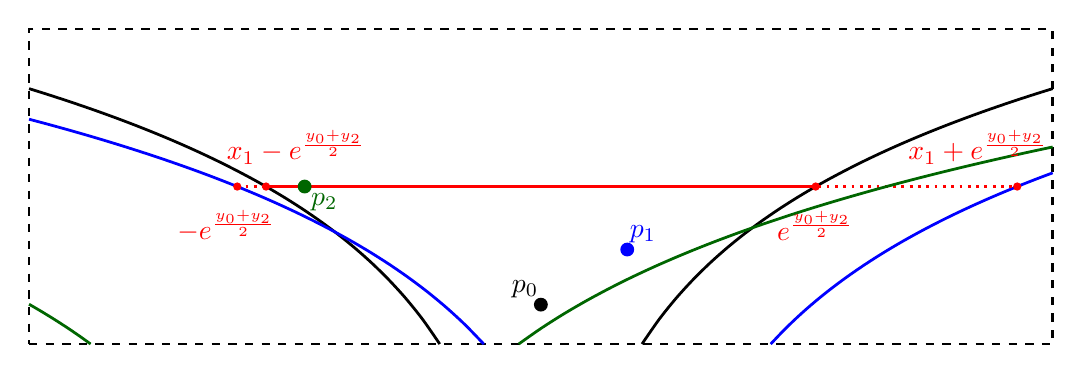
\begin{tikzpicture}
	%Define the coordinates 
	%p = (\u,\v) and p^\prime = (\uu, \vv)
	%Box \Rcal_n has width 2\r and height \t
	\pgfmathsetmacro{\u}{0} %0
	\pgfmathsetmacro{\v}{0.5} %1
	\pgfmathsetmacro{\vv}{1.2} %0.8
	\pgfmathsetmacro{\vvv}{2} %0.8
	\pgfmathsetmacro{\uuu}{-3} %1.4	
	\pgfmathsetmacro{\r}{6.5}
	\pgfmathsetmacro{\t}{4}
	
	\pgfmathsetmacro{\ubound}{exp((\vv+\vvv)/2)-exp((\v+\vvv)/2)}
	
	\pgfmathsetmacro{\uu}{3*\ubound/4}
	
	\pgfmathsetmacro{\leftintvandvvv}{-exp((\v + \vvv)/2)}
	\pgfmathsetmacro{\rightintvandvvv}{exp((\v + \vvv)/2)}
	\pgfmathsetmacro{\leftintvvandvvv}{\uu-exp((\vv + \vvv)/2)}
	\pgfmathsetmacro{\rightintvvandvvv}{\uu+exp((\vv + \vvv)/2)}
		
	%The box \Rcal_n
	\draw[line width=1pt,dashed] (-\r,0) -- (\r,0) -- (\r,\t) -- (-\r,\t) -- (-\r,0);

	%Dram all three nodes
    \draw node[fill, circle, inner sep=0pt, minimum size=5pt] (p1) at (\u,\v) {};
    \path (p1)+(-0.2,0.2) node {$p_0$};
    \draw node[fill,blue, circle, inner sep=0pt, minimum size=5pt] (p2) at (\uu,\vv) {};
    \path (p2)+(0.2,0.2) node {\color{blue}$p_1$};	
	
	%Boundaries p_0 = (\u,\v)
	
	%Right boundary
	\pgfmathsetmacro{\rightbounduv}{\u+exp((\v)/2)}
	\draw[domain=\rightbounduv:\r,smooth,variable=\x,black,line width=1pt] plot (\x, {2*ln(\x)-\v});
    %Left boundary
    \pgfmathsetmacro{\leftbounduv}{\u-exp((\v)/2)}
    \draw[domain=\leftbounduv:-\r,smooth,variable=\x,black,line width=1pt] plot (\x, {2*ln(-\x)-\v});
    
    %Boundaries p_1 = (\uu,\vv)
    
    %Right boundary
    \pgfmathsetmacro{\rightbounduuvv}{\uu+exp((\vv)/2)}
    \draw[domain=\rightbounduuvv:\r,smooth,variable=\x,blue,line width=1pt] plot (\x, {2*ln(\x-\uu)-\vv});
%    %Shifted right boundary
%    \pgfmathsetmacro{\shiftrightbounduuvv}{\uu+exp((\vv + \t)/2)-2*\r}
%    \draw[domain=\shiftrightbounduuvv:-\r,smooth,variable=\x,blue,line width=1pt] plot (\x, {2*ln(\x+(2*\r-\uu))-\vv});
    %Left boundary 
    \pgfmathsetmacro{\leftbounduuvv}{\uu-exp((\vv)/2)}
    \draw[domain=\leftbounduuvv:-\r,smooth,variable=\x,blue,line width=1pt] plot (\x, {2*ln(\uu-\x)-\vv});
%    %Shifted left boundary
%    \pgfmathsetmacro{\shiftleftbounduuvv}{\uu-exp((\vv + \t)/2)+2*\r}
%    \draw[domain=\shiftleftbounduuvv:\r,smooth,variable=\x,blue,line width=1pt] plot (\x, {2*ln(2*\r + \uu-\x)-\vv});
   


	\draw [red,dotted,line width=1pt] (\leftintvandvvv,\vvv) -- (\rightintvandvvv,\vvv);
	
	\draw [red,dotted,line width=1pt] (\leftintvvandvvv,\vvv) -- (\rightintvvandvvv,\vvv);

	\draw [red,line width=1pt] (\leftintvandvvv,\vvv) -- (\rightintvandvvv,\vvv);

    \draw node[fill,black!60!green, circle, inner sep=0pt, minimum size=5pt] (p2) at (\uuu,\vvv) {};
    \path (p2)+(0.25,-0.2) node {\color{black!60!green}$p_2$};
    
	%Boundaries p_2 = (\uuu,\vvv)
	
	%Right boundary
	\pgfmathsetmacro{\rightbounduuuvvv}{\uuu+exp((\vvv)/2)}
	\draw[domain=\rightbounduuuvvv:\r,smooth,variable=\x,black!60!green,line width=1pt] plot (\x, {2*ln(\x-\uuu)-\vvv});
    %Left boundary
    \pgfmathsetmacro{\leftbounduuuvvv}{\uuu-exp((\vvv)/2)}
    \draw[domain=\leftbounduuuvvv:-\r,smooth,variable=\x,black!60!green,line width=1pt] plot (\x, {2*ln(\uuu-\x)-\vvv});

	\draw node[fill,red, circle, inner sep=0pt, minimum size=3pt] at (\leftintvandvvv,\vvv) {};
	\path (\leftintvandvvv,\vvv)+(-0.5,-0.5) node[red] {$-e^{\frac{y_0 + y_2}{2}}$};
	\draw node[fill,red, circle, inner sep=0pt, minimum size=3pt] at (\rightintvandvvv,\vvv) {};
	\path (\rightintvandvvv,\vvv)+(0,-0.5) node[red] {$e^{\frac{y_0 + y_2}{2}}$};
	
	\draw node[fill,red, circle, inner sep=0pt, minimum size=3pt] at (\leftintvvandvvv,\vvv) {};
	\path (\leftintvvandvvv,\vvv)+(0.75,0.5) node[red] {$x_1 - e^{\frac{y_0 + y_2}{2}}$};
	\draw node[fill,red, circle, inner sep=0pt, minimum size=3pt] at (\rightintvvandvvv,\vvv) {};
	\path (\rightintvvandvvv,\vvv)+(-0.5,0.5) node[red] {$x_1 + e^{\frac{y_0 + y_2}{2}}$};

\end{tikzpicture}\\
\vspace{0.5cm}
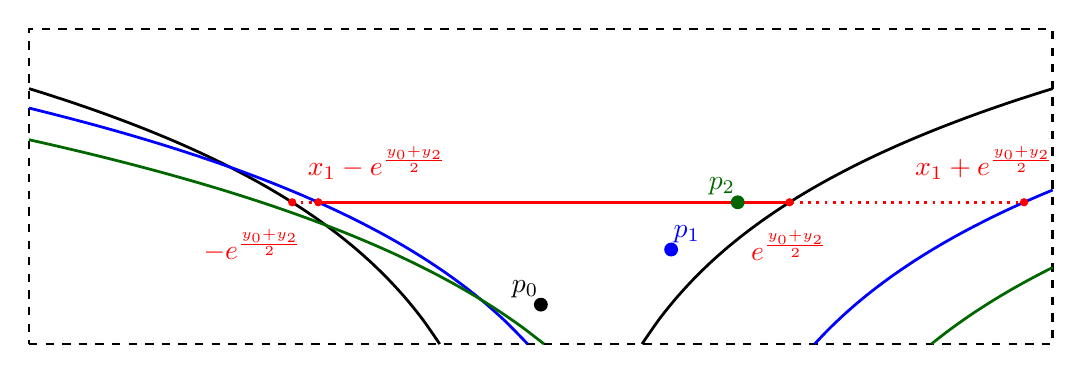
\begin{tikzpicture}
	%Define the coordinates 
	%p = (\u,\v) and p^\prime = (\uu, \vv)
	%Box \Rcal_n has width 2\r and height \t
	\pgfmathsetmacro{\u}{0} %0
	\pgfmathsetmacro{\v}{0.5} %1
	\pgfmathsetmacro{\vv}{1.2} %0.8
	\pgfmathsetmacro{\vvv}{1.8} %0.8
	\pgfmathsetmacro{\uuu}{2.5} %1.4	
	\pgfmathsetmacro{\r}{6.5}
	\pgfmathsetmacro{\t}{4}
	
	\pgfmathsetmacro{\ubound}{exp((\vv+\vvv)/2)-exp((\v+\vvv)/2)}
	
	\pgfmathsetmacro{\uu}{5*\ubound/4}
	
	\pgfmathsetmacro{\leftintvandvvv}{-exp((\v + \vvv)/2)}
	\pgfmathsetmacro{\rightintvandvvv}{exp((\v + \vvv)/2)}
	\pgfmathsetmacro{\leftintvvandvvv}{\uu-exp((\vv + \vvv)/2)}
	\pgfmathsetmacro{\rightintvvandvvv}{\uu+exp((\vv + \vvv)/2)}
		
	%The box \Rcal_n
	\draw[line width=1pt,dashed] (-\r,0) -- (\r,0) -- (\r,\t) -- (-\r,\t) -- (-\r,0);

	%Dram all three nodes
    \draw node[fill, circle, inner sep=0pt, minimum size=5pt] (p1) at (\u,\v) {};
    \path (p1)+(-0.2,0.2) node {$p_0$};
    \draw node[fill,blue, circle, inner sep=0pt, minimum size=5pt] (p2) at (\uu,\vv) {};
    \path (p2)+(0.2,0.2) node {\color{blue}$p_1$};	
	
	%Boundaries p_0 = (\u,\v)
	
	%Right boundary
	\pgfmathsetmacro{\rightbounduv}{\u+exp((\v)/2)}
	\draw[domain=\rightbounduv:\r,smooth,variable=\x,black,line width=1pt] plot (\x, {2*ln(\x)-\v});
    %Left boundary
    \pgfmathsetmacro{\leftbounduv}{\u-exp((\v)/2)}
    \draw[domain=\leftbounduv:-\r,smooth,variable=\x,black,line width=1pt] plot (\x, {2*ln(-\x)-\v});
    
    %Boundaries p_1 = (\uu,\vv)
    
    %Right boundary
    \pgfmathsetmacro{\rightbounduuvv}{\uu+exp((\vv)/2)}
    \draw[domain=\rightbounduuvv:\r,smooth,variable=\x,blue,line width=1pt] plot (\x, {2*ln(\x-\uu)-\vv});
    %Left boundary 
    \pgfmathsetmacro{\leftbounduuvv}{\uu-exp((\vv)/2)}
    \draw[domain=\leftbounduuvv:-\r,smooth,variable=\x,blue,line width=1pt] plot (\x, {2*ln(\uu-\x)-\vv});


	\draw [red,dotted,line width=1pt] (\leftintvandvvv,\vvv) -- (\rightintvandvvv,\vvv);
	
	\draw [red,dotted,line width=1pt] (\leftintvvandvvv,\vvv) -- (\rightintvvandvvv,\vvv);

	\draw [red,line width=1pt] (\leftintvvandvvv,\vvv) -- (\rightintvandvvv,\vvv);
	


    \draw node[fill,black!60!green, circle, inner sep=0pt, minimum size=5pt] (p2) at (\uuu,\vvv) {};
    \path (p2)+(-0.2,0.2) node {\color{black!60!green}$p_2$};
    
	%Boundaries p_2 = (\uuu,\vvv)
	
	%Right boundary
	\pgfmathsetmacro{\rightbounduuuvvv}{\uuu+exp((\vvv)/2)}
	\draw[domain=\rightbounduuuvvv:\r,smooth,variable=\x,black!60!green,line width=1pt] plot (\x, {2*ln(\x-\uuu)-\vvv});
    %Left boundary
    \pgfmathsetmacro{\leftbounduuuvvv}{\uuu-exp((\vvv)/2)}
    \draw[domain=\leftbounduuuvvv:-\r,smooth,variable=\x,black!60!green,line width=1pt] plot (\x, {2*ln(\uuu-\x)-\vvv});

	\draw node[fill,red, circle, inner sep=0pt, minimum size=3pt] at (\leftintvandvvv,\vvv) {};
	\path (\leftintvandvvv,\vvv)+(-0.5,-0.55) node[red] {$-e^{\frac{y_0 + y_2}{2}}$};
	\draw node[fill,red, circle, inner sep=0pt, minimum size=3pt] at (\rightintvandvvv,\vvv) {};
	\path (\rightintvandvvv,\vvv)+(0,-0.55) node[red] {$e^{\frac{y_0 + y_2}{2}}$};
	
	\draw node[fill,red, circle, inner sep=0pt, minimum size=3pt] at (\leftintvvandvvv,\vvv) {};
	\path (\leftintvvandvvv,\vvv)+(0.75,0.5) node[red] {$x_1 - e^{\frac{y_0 + y_2}{2}}$};
	\draw node[fill,red, circle, inner sep=0pt, minimum size=3pt] at (\rightintvvandvvv,\vvv) {};
	\path (\rightintvvandvvv,\vvv)+(-0.5,0.5) node[red] {$x_1 + e^{\frac{y_0 + y_2}{2}}$};

\end{tikzpicture}
\caption{Situation for the intersections of the connection intervals considered in Lemma~\ref{lem:ordered}, with $y_0 < y_1 <y_2$ fixed and for different cases of $0 \le x_1 \le e^{(y_0 + y_1)/2}$. The top figure shows the case where $0 \le x_1 \le e^{(y_1 + y_2)/2} - e^{(y_0 + y_2)/2}$, while the bottom one shows the case $x_1 > e^{(y_1 + y_2)/2} - e^{(y_0 + y_2)/2}$. The solid red line indicates the range for $x_2$ such that the points $p_0$, $p_1$ and $p_2$ form a triangle. The boundaries of their neighborhoods are shown in, respectively, black, blue and green.}
\label{fig:triangle_prob_lemma}
\end{figure}

\begin{proof}
Note that $P(y_0,y_1,y_2)$ is the probability that $x_2$ falls into the interval $[x_1-e^{(y_1+y_2)/2},x_1+e^{(y_1+y_2)/2}]$, as well as into the interval $[-e^{(y_0+y_2)/2},e^{(y_0+y_2)/2}]$. By symmetry considerations, we can take $x_1$ uniformly at random from $[0,e^{y_0/2+y_1/2}]$ as opposed to $[-e^{y_0/2+y_1/2}, e^{y_0/2+y_1/2}]$. Figure~\ref{fig:triangle_prob_lemma} shows the intersection of the intervals (red line) for two different cases for $x_1 \le e^{(y_0 + y_1)/2}$. 

Since $y_0 < y_1 < y_2$ we have that $e^{(y_1+y_2)/2} > e^{(y_0+y_2)/2}$ and so, when $x_1 \geq 0$, the ``right half'' of the 
interval $[-e^{(y_0+y_2)/2}, e^{(y_0+y_2)/2}]$ is always covered by the interval $[x_1-e^{(y_1+y_2)/2}, x_1+e^{(y_1+y_2)/2}]$.
If $e^{(y_1+y_2)/2} - e^{(y_0+y_1)/2} \geq e^{(y_0+y_2)/2}$ then the ``left half'' is always covered as well.
In other words:
\[
	e^{(y_1+y_2)/2} - e^{(y_0+y_1)/2} \geq e^{(y_0+y_2)/2} \Rightarrow P(y_0,y_1,y_2) = 1.
\]

Now consider the case where $e^{(y_1+y_2)/2} - e^{(y_0+y_1)/2} < e^{(y_0+y_2)/2}$. 
Then, if $x_1 \in [0, e^{(y_1+y_2)/2} - e^{(y_0+y_2)/2}]$ the whole interval $[-e^{(y_0+y_2)/2}, e^{(y_0+y_2)/2}]$ is still covered 
so that $p_0, p_1$ and $p_2$ form a triangle. If, on the other hand $e^{(y_1+y_2)/2} - e^{(y_0+y_2)/2} < x_1 \leq e^{(y_0+y_1)/2}$ then
the probability that $|x_2-x_1| \leq e^{(y_1+y_2)/2}$ equals
\[ 
	1 - \frac{x_1 - (e^{(y_1+y_2)/2} - e^{(y_0+y_2)/2)}) }{ 2e^{(y_0+y_2)/2} }. 
\]

Hence, when $e^{(y_1+y_2)/2} - e^{(y_0+y_1)/2} < e^{(y_0+y_2)/2}$ we have
\begin{align*}
	P(y_0,y_1,y_2) &= \frac{e^{(y_1+y_2)/2} - e^{(y_0+y_2)/2} }{ e^{(y_0+y_1)/2} }  \\
	&\hspace{10pt}+ \int_{ e^{(y_1+y_2)/2} - e^{(y_0+y_2)/2} }^{ e^{(y_0+y_1)/2} } 
	    \left(1 - \frac{x_1 - (e^{(y_1+y_2)/2} - e^{(y_0+y_2)/2)}) }{ 2e^{(y_0+y_2)/2} }\right)
	    \cdot \frac{1}{e^{(y_0+y_1)/2}} \dd x_1 \\
	&= 1 - \frac{1}{2e^{y_0+y_1/2+y_2/2} } \int_0^{ e^{(y_0+y_1)/2}+e^{(y_0+y_2)/2}-e^{(y_1+y_2)/2} } x_1 \dd x_1 \\
	&= 1 - \frac{ \left( e^{(y_0+y_1)/2}+e^{(y_0+y_2)/2}-e^{(y_1+y_2)/2} \right)^2 }{ 4 e^{y_0+y_1/2+y_2/2} },
\end{align*}

At this point it is convenient to rewrite everything in terms of $z_i := e^{-y_i/2}$.
Note that $y_0 < y_1 < y_2$ if and only if $z_0 > z_1 > z_2$ while the condition $e^{(y_1+y_2)/2} - e^{(y_0+y_1)/2} < e^{(y_0+y_2)/2}$ becomes
\[ e^{(y_1+y_2)/2} - e^{(y_0+y_1)/2} < e^{(y_0+y_2)/2} \Leftrightarrow 
z_1^{-1} z_2^{-1} < z_0^{-1} z_1^{-1} + z_0^{-1}z_2^{-1} 
\Leftrightarrow
z_0 < z_1+z_2. 
\]

We now conclude that
\[
	P(y_0(z_0), y_1(z_1), y_2(z_2)) = 1 \quad \text{if} \quad z_0 > z_1 > z_2 \text{ and } z_0 \geq z_1 + z_2
\]
while for $z_0 > z_1 > z_2$ and $z_0 < z_1 + z_2$
\begin{align*}
	P(y_0(z_0), y_1(z_1), y_2(z_2)) 
	&= 1 - \frac{z_0^2z_1z_2}{4} \cdot \left( z_0^{-1}z_1^{-1}+z_0^{-1}z_2^{-1}-z_1^{-1}z_2^{-1} \right)^2 \\
%	&= 1 - \frac{z_0^2z_1z_2}{4} \cdot \left( z_0^{-2}z_1^{-2} + z_0^{-2}z_2^{-2} + z_1^{-2}z_2^{-2}
%		+ 2z_0^{-2}z_1^{-1}z_2^{-1} - 2 z_0^{-1}z_1^{-2}z_2^{-1} - 2z_0^{-1}z_1^{-1}z_2^{-2} \right) \\
	&= 1 - \frac{1}{4} \left( z_1^{-1}z_2 + z_1z_2^{-1} + z_0^2z_1^{-1}z_2^{-1} + 2 - 2z_0z_1^{-1}-2z_0z_2^{-1}\right),
\end{align*}
which finishes the proof.
\end{proof}

The previous lemma covers the case when $y_0<y_1<y_2$. We now leverage it to take care of the other cases as well. 

\begin{proof}[Proof of Lemma~\ref{lem:triangle_prob_y_coordinates}]
Let $y_i >0$ and $z_i = e^{-y_i/2}$, $i=0,1,2$. Lemma~\ref{lem:ordered} gives the expression for $P(y_0(z_0),y_1(z_1),y_2(z_2))$ in the case $y_0<y_1<y_2$, or equivalently $z_0>z_1>z_2$, i.e. the first two lines in the claim of Lemma~\ref{lem:triangle_prob_y_coordinates}. To analyze the other cases we shall express $P(y_1,y_0,y_2)$ and $P(y_1,y_2,y_0)$ in terms of $P(y_0,y_1,y_2)$ and $z_i$. For this we note that we can view $P(y_0,y_1,y_2)$ as a 2-fold integral of the indicator function
\[ 
	h(x_0, x_1, x_2) := \ind{ |x_0 - x_1| < e^{(y_0+y_1)/2}, |x_0 - x_2| < e^{(y_0+y_2)/2}, |x_1-x_2| < e^{(y_1+y_2)/2}}, 
\]
where $x_0$ was set to zero, without loss of generality, and the other two $x_i$ are uniform random variables on $[-e^{(y_0+y_i)/2}, e^{(y_0+y_i)/2}]$. When we consider the probability $P(y_1,y_0,y_2)$, this is the 2-fold integral of $h(x_0,0,x_2)$ so that
\begin{align*}
	P(y_1,y_0,y_2) &= \frac{1}{2e^{(y_1+y_0)/2}} \cdot \frac{1}{2e^{(y_1+y_2)/2}} 
		\iint_{\R} h(x_0,0,x_2) \dd x_0 \dd x_2\\
	&= \frac{e^{y_0/2}}{e^{y_1/2}} \frac{1}{2e^{(y_0+y_1)/2}} \frac{1}{2e^{(y_0+y_2)/2}} 
		\iint_{\R} h(0,x_1,x_2) \dd x_1 \dd x_2\\
	&= \frac{e^{y_0/2}}{e^{y_1/2}} P(y_0,y_1,y_2) = \frac{z_1}{z_0}  P(y_0,y_1,y_2).
\end{align*}
Finally we note that $h(x_0,0,x_2) = h(x_2,0,x_0)$ from which we conclude that
\begin{equation}\label{eq:symmetry_relation_triangle_prob}
	P(y_0, y_1, y_2) = \left(z_0/z_1\right) P(y_1,y_0,y_2) = \left(z_0/z_1\right) P(y_1,y_2,y_0).
\end{equation}

To complete the proof for the other cases we note that since $P(y_0,y_1,y_2)$ is symmetric in $y_1$ and $y_2$, we can assume, without loss of generality, that $y_1 < y_2$. Then, there are two more orderings of $y_0, y_1, y_2$, namely $y_1< y_0< y_2$ and $y_1<y_2<y_0$, which can be summarized as $y_1 < \min (y_0,y_2)$, or equivalently $z_1 > \max(z_0,z_2)$. For $y_1 < y_0 < y_2$ and $y_1 < y_2<y_0$ we can apply Lemma~\ref{lem:ordered} to obtain $P(y_1,y_0,y_2) = P(y_1,y_2,y_0)$ which happen to agree due to the symmetry in the last two arguments of the expression found in Lemma~\ref{lem:ordered}. The expression for $P(y_0,y_1,y_2)$ then follows from~\eqref{eq:symmetry_relation_triangle_prob}.
\end{proof}

%


\subsubsection{Integrating over $y_1, y_2$}


Now that we have established the expression for $P(y_0,y_1,y_2)$ we can proceed to compute $P(y_0)$ by integrating over $y_1, y_2$.
We however start with the following observation.

\begin{lemma}\label{lem:continuity_Delta_function}
The function $\alpha \mapsto P_\alpha(y_0)$ is continuous for all $\alpha > \frac{1}{2}$.
\end{lemma}

\begin{proof}
This follows from the theorem of dominated convergence:
Let $\alpha > \frac{1}{2}$ and $(\alpha_n)_{n\in \mathbb{N}}$ a sequence of real numbers converging to $\alpha$, so we can 
assume $|\alpha_n - \alpha| < \epsilon := \frac{\alpha-1/2}{2}$. 
This means that $-\epsilon < \alpha_n - \alpha < \epsilon$, i.e. $\frac{\alpha-1/2}{2} < \alpha_n - 1/2 < \frac{3\alpha-3/2}{2}$. Define 

$$f_n(y_1,y_2) = P(y_0,y_1,y_2) (\alpha_n - 1/2)^2 e^{-(\alpha_n-1/2)(y_1+y_2)}.$$ 

As the function $x \mapsto x^2$ is increasing in $x$ for $x>0$ and the function $x \mapsto e^{-(y_1+y_2)x}$ is decreasing 
in $x$ and $P(y_0,y_1,y_2) \in [0,1]$, it holds that 

$$|f_n(y_1,y_2)| \leq \left(\frac{3\alpha-3/2}{2}\right)^2e^{-(y_1+y_2)\frac{\alpha-1/2}{2}}$$

which is integrable over $\R_{\geq 0} \times \R_{\geq 0}$ (with integral equalling $(6\alpha-3)^2/(2\alpha-1)^2$). 
Application of the theorem of dominated convergence yields that 
$P_{\alpha_n}(y_0) \rightarrow P_\alpha(y_0)$ which gives the claim as the 
sequence $(\alpha_n)_n$ was arbitrary.
\end{proof}

Due to this lemma we can first assume $\alpha \notin \{ \frac{3}{4},1 \}$, compute $P(y_0)$ and then obtain the values of $P(y_0)$ at 
the remaining two points by taking the corresponding limit in $\alpha$. 
This strategy is executed below. 
It involves the computation of several integrals which are involved and will take up a few pages. 
The proof is structured using headers, to aid the reader. 


%\begin{proof}[Proof of Proposition~\ref{prop:full_expression_delta_P}]\hfill


%\paragraph{When $\bm{\alpha \notin \{3/4,1\}}$}

Note that when writing $P(y_0)$ as an integral, see equation~\eqref{eq:delta_P}, by symmetry in the integration 
variables $y_1$ and $y_2$, we can assume that $y_1<y_2$ in which case either $y_0$ or $y_1$ is the smallest height. 
This gives half the value of $P(y_0)$ and hence
\[ 
	P(y_0) = 2(I_1(y_0) +I_2(y_0)), 
\] 
where $I_1$ and $I_2$ are given by:
\begin{align*}
	I_1(y_0) &:= \int_{0<y_0<y_1<y_2} P(y_0,y_1,y_2) \cdot (\alpha-1/2)^2 e^{-(\alpha-1/2)(y_1+y_2)}  \dd y_2 \dd y_1 \\ 
	I_2(y_0) &:= \int_{0<y_1<y_0,y_2} P(y_0,y_1,y_2) \cdot (\alpha-1/2)^2 e^{-(\alpha-1/2)(y_1+y_2)} \dd y_2 \dd y_1 \\ 
\end{align*}

We proceed with computing each of these two integrals, each of which is split in two parts. 
The final expressions of those four integrals can be found 
in~\eqref{eq:Delta_P_computation_I11}, \eqref{eq:Delta_P_computation_I12}, \eqref{eq:Delta_P_computation_I21} 
and~\eqref{eq:Delta_P_computation_I22}.

\paragraph{Computing $\bm{I_1(y_0)}$}

Applying the change of variables $z_i := e^{-y_i/2}$, $i=1,2$, and Lemma~\ref{lem:triangle_prob_y_coordinates} gives %${\dd}y_i = -\frac{2{\dd}z_i}{z_i}$ and therefore
\begin{align*}
	I_1(y_0) &=	4 (\alpha-1/2)^2 \cdot \int_{z_0>z_1>z_2>0} P(y_0,y_1(z),y_2(z)) z_1^{2\alpha-2} z_2^{2\alpha-2} 
		{\dd}z_2{\dd}z_1 \\
	&= 4 (\alpha-1/2)^2 \cdot \left( \int_{z_0>z_1>z_2>0} 1 \cdot z_1^{2\alpha-2} z_2^{2\alpha-2} 
		{\dd}z_2{\dd}z_1 \right. \\
	&\hspace{10pt} \left. - \int_{{z_0>z_1>z_2>0,}\atop{z_0 < z_1+z_2}} G(z_0,z_1,z_2) \cdot z_1^{2\alpha-2} z_2^{2\alpha-2} 
		{\dd}z_2{\dd}z_1 \right) \\
	&=: 4 (\alpha-1/2)^2 ( I_{11}(y_0) - I_{12}(y_0)). 
\end{align*}

The integral $I_{11}(y_0)$ is easily obtained:
\begin{align*}
	I_{11}(y_0) &= \int_0^{z_0} \int_0^{z_1} z_1^{2\alpha-2} z_2^{2\alpha-2} {\dd}z_2{\dd}z_1
		= \int_0^{z_0} z_1^{2\alpha-2} \left[ \frac{z_2^{2\alpha-1}}{2\alpha-1} \right]_0^{z_1} {\dd}z_1\\
	&= \frac{1}{2\alpha-1} \cdot \int_0^{z_0} z_1^{4\alpha-3} {\dd}z_1
		= \frac{1}{2(2\alpha-1)^2} \cdot z_0^{4\alpha-2}. \numberthis \label{eq:Delta_P_computation_I11}
\end{align*}

To deal with $I_{12}$ we note that $G(z_0,z_1,z_2)$ is a linear combination of monomials of the form $z_0^az_1^bz_2^c$ with 
$a,b,c \in \{-1,0,1,2\}$ and $a+b+c=0$. Let us consider the integral $J_{(a,b,c)}(z_0)$ defined by 

\begin{equation}\label{eq:def_Delta_P_computation_int_J_1}
	J_{a,b,c}(z_0) := z_0^a \int_{{z_0>z_1>z_2>0,}\atop{z_0 < z_1+z_2}} z_1^{b+2\alpha-2} z_2^{c+2\alpha-2} {\dd}z_2{\dd}z_1.
\end{equation}
and note that
\begin{equation}\label{eq:Delta_P_computation_I12_with_J}
	I_{1,2}(y_0) = \frac{1}{4} (J_{0,-1,1}(z_0)+J_{0,1,-1}(z_0)+J_{2,-1,-1}(z_0)+2J_{0,0,0}(z_0)-2J_{1,-1,0}(z_0)-2J_{1,0,-1}(z_0)).
\end{equation}

Next we compute $J_{a,b,c}(z_0)$.
\begin{align*}
	J_{a,b,c}(z_0) 
	&= z_0^a \int_{z_0/2}^{z_0}\int_{z_0-z_1}^{z_1} z_1^{b+2\alpha-2} z_2^{c+2\alpha-2} {\dd}z_2{\dd}z_1
		= z_0^a \int_{z_0/2}^{z_0} z_1^{b+2\alpha-2} \left[ \frac{ z_2^{c+2\alpha-1} }{ c+2\alpha-1 } \right]_{z_0-z_1}^{z_1} \dd z_1\\
	&= \frac{z_0^a}{c+2\alpha-1} \cdot \left( \int_{z_0/2}^{z_0} z_1^{b+c+4\alpha-3} \dd z_1
	   - \int_{z_0/2}^{z_0} z_1^{b+2\alpha-2} (z_0-z_1)^{c+2\alpha-1} {\dd}z_1 \right) \\
	&= \frac{z_0^{a+b+c+4\alpha-2}(1-(1/2)^{b+c+4\alpha-2})}{(c+2\alpha-1)(b+c+4\alpha-2)} \\
	&\hspace{10pt}- \frac{z_0^{a+b+c+4\alpha-3}}{c+2\alpha-1} \int_{z_0/2}^{z_0}  \left(z_1/z_0\right)^{b+2\alpha-2} 
	    \left(1-(z_1/z_0)\right)^{c+2\alpha-1} \dd z_1\\
	&= \frac{z_0^{4\alpha-2}(1-(1/2)^{b+c+4\alpha-2})}{(c+2\alpha-1)(b+c+4\alpha-2)} 
		- \frac{z_0^{4\alpha-2}}{c+2\alpha-1}
	   \int_{1/2}^1  u^{b+2\alpha-2}(1-u)^{c+2\alpha-1} \dd u \\
	&= \frac{z_0^{4\alpha-2}(1-(1/2)^{b+c+4\alpha-2})}{(c+2\alpha-1)(b+c+4\alpha-2)} 
		- \frac{z_0^{4\alpha-2}}{c+2\alpha-1} B^-(1/2;c+2\alpha, b+2\alpha-1),
\end{align*}
where we have used the substitution $u := z_1/z_0$ giving $z_0 {\dd} u = {\dd} z_1$ in the penultimate line and
$B^-$ denotes the (lower) incomplete beta function. Note that since $c \geq -1$, $-a \in \{0,-1,-2\}$ and by our assumption $\alpha \not \in \{\frac{3}{4},1\}$, the denominators that occur during the integration are all non-zero.

Plugging this back into~\eqref{eq:Delta_P_computation_I12_with_J} gives
\begin{align*}
	I_{1,2}(y_0)
	&= \frac{z_0^{4\alpha-2}(1-(1/2)^{4\alpha-2})}{32\alpha(\alpha-1/2)} 
   		- \frac{z_0^{4\alpha-2}}{8\alpha} B^-(1/2;1+2\alpha, 2\alpha-2)\\
	&\hspace{10pt}+ \frac{z_0^{4\alpha-2}(1-(1/2)^{4\alpha-2})}{32(\alpha-1)(\alpha-1/2)} 
   		-  \frac{z_0^{4\alpha-2}}{4(2\alpha-2)} B^-(1/2;2\alpha-1,2\alpha)\\
	&\hspace{10pt}+ \frac{z_0^{4\alpha-2}(1-(1/2)^{4\alpha-4})}{32(\alpha-1)^2} 
   		- \frac{z_0^{4\alpha-2}}{4(2\alpha-2)} B^-(1/2;-1+2\alpha, 2\alpha-2)\\
	&\hspace{10pt}+ \frac{z_0^{4\alpha-2}(1-(1/2)^{4\alpha-2})}{16(\alpha-1/2)^2} 
   		- \frac{z_0^{4\alpha-2}}{2(2\alpha-1)} B^-(1/2;2\alpha,2\alpha-1)\\
	&\hspace{10pt}- \frac{z_0^{4\alpha-2}(1-(1/2)^{4\alpha-3})}{16(\alpha-1/2)(\alpha-3/4)} 
   		+ \frac{z_0^{4\alpha-2}}{2(2\alpha-1)} B^-(1/2;2\alpha, 2\alpha-2)\\
	&\hspace{10pt}- \frac{z_0^{4\alpha-2}(1-(1/2)^{4\alpha-3})}{16(\alpha-1)(\alpha-3/4)} 
   		+ \frac{z_0^{4\alpha-2}}{2(2\alpha-2)} B^-(1/2;-1+2\alpha, 2\alpha-1) \\
	&=\frac{\left(\frac{3}{64}- \frac{3}{16} 2^{-4\alpha}+ 
   		\alpha (-\frac{41}{128} + \frac{13}{16}  2^{-4\alpha}) 
   		+ \alpha^2 (\frac{5}{8} - \frac{3}{4} 2^{-4\alpha}) - \frac{15}{32}\alpha^3 +\frac{1}{8} a^4\right) 
   		z_0^{4 \alpha-2} }{4(\alpha-1/2)^2 (\alpha-1)^2 (\alpha-3/4) \alpha} \\
	&\hspace{10pt}+ \frac{z_0^{4\alpha-2}}{8 (\alpha-1) \alpha (2\alpha-1)}(4 (\alpha-1) \alpha 
		(B^-(1/2; 2\alpha, 2\alpha-2) - B^-(1/2;2 \alpha,2\alpha-1) ) \\
    &\hspace{10pt}- (2 \alpha-1)\alpha ( B^-(1/2; 2\alpha-1, 2\alpha-2) + 
    	B^-(1/2; 2\alpha-1, 2\alpha) - 
    	2 B^-(1/2;2\alpha -1, 2\alpha-1) ) \\
    &\hspace{10pt}- (2\alpha-1)(\alpha-1) B^-(1/2; 1 + 2\alpha, 2\alpha-2)) \\
	&=\frac{\left(\frac{3}{64}- \frac{3}{16} 2^{-4\alpha} 
		+ \alpha (-\frac{41}{128} + \frac{13}{16}  2^{-4\alpha})  
		+ \alpha^2 (\frac{5}{8} - \frac{3}{4} 2^{-4\alpha}) - \frac{15}{32}\alpha^3 +\frac{1}{8} a^4\right) 
		z_0^{4 \alpha-2} }{4(\alpha-1/2)^2 (\alpha-1)^2 (\alpha-3/4) \alpha} \\
 	&\hspace{10pt}+ \frac{z_0^{4\alpha-2}}{8 (\alpha-1) \alpha (2\alpha-1)}(4 (\alpha-1) \alpha 
 		B^-(1/2; 2\alpha+1, 2\alpha-2) \\
  	&\hspace{10pt}- (2 \alpha-1)\alpha B^-(1/2;2\alpha+1,2\alpha-2) \\
    &\hspace{10pt}- (2\alpha-1)(\alpha-1) B^-(1/2; 2\alpha+1, 2\alpha-2)). \\
\end{align*}
For the last step we use the identities 
\begin{align}
	B^-(z;a,b)-B^-(z;a,b+1) &= B^-(z; a+1,b), \label{eq:Delta_P_computation_beta_id_1}\\
	B^-(z;a,b)+B^-(z;a,b+2)-2B^-(z;a,b+1) &= B^-(z;a+2,b). \label{eq:Delta_P_computation_beta_id_2}
\end{align}
to obtain
\begin{equation}
\begin{aligned}
	I_{1,2}(y_0) &=\frac{\left(\frac{3}{64}- \frac{3}{16} 2^{-4\alpha}
		+ \alpha (-\frac{41}{128} + \frac{13}{16}  2^{-4\alpha})
		+ \alpha^2 (\frac{5}{8} - \frac{3}{4} 2^{-4\alpha}) - \frac{15}{32}\alpha^3 +\frac{1}{8} a^4\right) 
		z_0^{4 \alpha-2} }{4(\alpha-1/2)^2 (\alpha-1)^2 (\alpha-3/4) \alpha} \\
 	&\hspace{10pt}- \frac{z_0^{4\alpha-2}B^-(1/2; 2\alpha+1, 2\alpha-2) }{8 (\alpha-1) \alpha (2\alpha-1)}	\label{eq:Delta_P_computation_I12}
\end{aligned}
\end{equation}


\paragraph{Computing $\bm{I_2(y_0)}$}

We will follow a similar strategy as for $I_1(y_0)$. First, using the change of variables $z_i := e^{-y_i/2}$, $i=1,2$,
we get
\begin{align*}
	I_2(y_0) &= 4 (\alpha-1/2)^2 \cdot \int_{1>z_1>z_2,z_0>0} P(y_0,y_1(z_1),y_2(z_2)) z_1^{2\alpha-2} z_2^{2\alpha-2} 
		{\dd}z_2{\dd}z_1 \\
	&= 4 (\alpha-1/2)^2 \cdot \left( \int_{1>z_1>z_0,z_2>0}  z_0 z_1^{2\alpha-3} z_2^{2\alpha-2} 
		{\dd}z_2{\dd}z_1 \right. \\
	&\hspace{10pt}\left. - \int_{{1>z_1>z_0,z_2>0}\atop{z_1 < z_0+z_2}} G(z_1,z_0,z_2) z_0 z_1^{2\alpha-3} 	
		z_2^{2\alpha-2} \dd z_2{\dd}z_1 \right) \\
	&=: 4 (\alpha-1/2)^2 (I_{21}(y_0) - I_{22}(y_0)). 
\end{align*}

We proceed with the easy integral:
\begin{align*}
	I_{21}(y_0) &= z_0 \int_{1>z_1>\max(z_2,z_0);z_0,z_2>0} z_1^{2\alpha-3} z_2^{2\alpha-2} {\dd}z_2{\dd}z_1   
		= z_0 \int_{z_0}^1 \int_{0}^{z_1} z_1^{2\alpha-3} z_2^{2\alpha-2} {\dd}z_2{\dd}z_1\\
	&= z_0 \int_{z_0}^1 \left[ \frac{z_2^{2\alpha-1}}{2\alpha-1}\right]_{0}^{z_1} z_1^{2\alpha-3} {\dd}z_1 
		= \frac{z_0}{2\alpha-1}  \int_{z_0}^1 z_1^{4\alpha-4} {\dd}z_1
		= \frac{z_0 - z_0^{4\alpha-2}}{(4\alpha-3)(2\alpha-1)}. \numberthis \label{eq:Delta_P_computation_I21}
\end{align*}
We note that the denominators above are non-zero as $\alpha > \frac{1}{2}$ and $\alpha \not =\frac{3}{4}$.

To deal with $I_{22}(y_0)$ we consider the integral function
\[
	J_{a,b,c}^\prime(z_0) := z_0^a \int_{{1>z_1>\max(z_0,z_2); z_0,z_2>0}\atop{z_1 < z_0+z_2}} z_1^{b+2\alpha-2} z_2^{c+2\alpha-2} {\dd}z_2{\dd}z_1
\]
and note that
\begin{equation}\label{eq:Delta_P_computation_I22_J}
\begin{aligned}
		I_{2,2}(y_0) &= \frac{1}{4}\left(J_{0,-1,1}^\prime(z_0) + J_{2,-1,-1}^\prime(z_0)
		+ J_{0,1,-1}^\prime(z_0)\right) \\
		&\hspace{10pt}+ \frac{1}{2}\left( J_{1,-1,0}^\prime(z_0) - J_{0,0,0}^\prime(z_0) - J_{1,0,-1}^\prime(z_0)\right).
\end{aligned}
\end{equation}

We now compute $J_{a,b,c}^\prime(z_0)$
\begin{align*}
	J_{a,b,c}^\prime(z_0) 
	&= z_0^a \int_{z_0}^1 \int_{z_1-z_0}^{z_1}  z_1^{b+2\alpha-2} z_2^{c+2\alpha-2} {\dd} z_2 {\dd} z_1  \\
 	&= z_0^a \int_{z_0}^1 \frac{1}{c+2\alpha-1}  z_1^{b+2\alpha-2}( z_1^{c+2\alpha-1}-(z_1-z_0)^{c+2\alpha-1})  {\dd} z_1  \\
 	&=z_0^a \int_{z_0}^1 \frac{1}{c+2\alpha-1} z_1^{b+c+4\alpha-3} {\dd } z_1 -z_0^{a} \int_{z_0}^1 	
 		\frac{1}{c+2\alpha-1}z_1^{b+2\alpha-2}(z_1-z_0)^{c+2\alpha-1}  {\dd} z_1  \\
 	&= z_0^a  \frac{1}{(c+2\alpha-1)(b+c+4\alpha-2)}(1-z_0^{b+c+4\alpha-2}) \\
 	&\hspace{10pt}- \frac{z_0^a}{c+2\alpha-1}z_0^{b+c+4\alpha-2}B^-(1-z_0;c+2\alpha,-b-c-4\alpha+2) \\
	&= \frac{z_0^a -z_0^{4\alpha-2}}{(c+2\alpha-1)(b+c+4\alpha-2)}  
		- \frac{z_0^{4\alpha -2}B^-(1-z_0;c+2\alpha,-b-c-4\alpha+2)}{c+2\alpha-1}.  
\end{align*}
Here we used that for $x  \in \R,y>-1$ (note that as $c\geq -1$, it holds that $c+2\alpha-1 >-1$):
\begin{align*}
 \int_{z_0}^{1} z_1^x (z_1-z_0)^y {\dd} z_1 
 &= \int_0^{1-z_0} (s+z_0)^x s^y {\dd} s \\
 &= z_0^{x+y} \int_0^{1-z_0} \left( (s/z_0) + 1 \right)^x (s/z_0)^y {\dd} s \\
 &= z_0^{x+y+1} \int_{0}^{1/z_0 -1 } (t+1)^x t^y {\dd} t \\
 &= z_0^{x+y+1} \int_0^{1-z_0} u^y (1-u)^{-(x+y+2)} {\dd} u \\
 &= z_0^{x+y+1} B^-(1-z_0; y+1,-x-y-1 ).
\end{align*}
As $c \geq -1$ and $-a \in \{0,-1,-2\}$ and by our assumption $\alpha \not \in \{\frac{3}{4}\}$, the denominators 
that occur during the computations above are non-zero. 

Plugging the expression for $J_{a,b,c}^\prime(z_0)$ back into~\eqref{eq:Delta_P_computation_I22_J} we get,
\begin{align*}
	I_{2,2}(y_0) 
	&= \frac{1 -z_0^{4\alpha-2}}{32\alpha(\alpha-1/2)} 
		-  \frac{z_0^{4\alpha -2}B^-(1-z_0;1+2\alpha,-4\alpha+2)}{8\alpha} \\
	&\hspace{10pt}+ \frac{z_0^2 -z_0^{4\alpha-2}}{32(\alpha-1)^2}  
		- \frac{z_0^{4\alpha -2}B^-(1-z_0;-1+2\alpha,-4\alpha+4)}{8(\alpha-1)} \\
	&\hspace{10pt}+ \frac{1 -z_0^{4\alpha-2}}{32(\alpha-1)(\alpha-1/2)}  
		- \frac{z_0^{4\alpha -2}B^-(1-z_0;-1+2\alpha,-4\alpha+2)}{8(\alpha-1)} \\
	&\hspace{10pt}+ \frac{z_0 -z_0^{4\alpha-2}}{16(\alpha-1/2)(\alpha-3/4)}  
		- \frac{z_0^{4\alpha -2}B^-(1-z_0;2\alpha,-4\alpha+3)}{4(\alpha-1/2)} \\
	&\hspace{10pt}- \frac{1 -z_0^{4\alpha-2}}{16(\alpha-1/2)^2}  
		+ \frac{z_0^{4\alpha -2}B^-(1-z_0;2\alpha,-4\alpha+2)}{4(\alpha-1/2)}\\
	&\hspace{10pt}-\frac{z_0 -z_0^{4\alpha-2}}{16(\alpha-1)(\alpha-3/4)} 
		+ \frac{z_0^{4\alpha -2}B^-(1-z_0;-1+2\alpha,-4\alpha+3)}{4(\alpha-1)}.
\end{align*}
Using some algebra and the identities~\eqref{eq:Delta_P_computation_beta_id_1} and~\eqref{eq:Delta_P_computation_beta_id_2}  
this can be reduced to
\begin{equation}\label{eq:Delta_P_computation_I22}
\begin{aligned}
	I_{2,2}(y_0)
	&=\frac{1}{64\alpha(\alpha-1/2)^2(\alpha-1)} -\frac{(1 - z_0)^{2\alpha}}{64\alpha(\alpha-1/2)^2 (\alpha-1)} 
		- \frac{z_0}{8(\alpha-1/2)(\alpha-1)(4\alpha-3)}\\ 
	&\hspace{10pt}+ \frac{z_0^2}{32(\alpha-1)^2} + \frac{(-6 + 25\alpha - 48\alpha^2 + 44\alpha^3 -16\alpha^4) 
   		z_0^{4\alpha-2}}{512\alpha(\alpha-1/2)^2(\alpha-1)^2(\alpha-3/4)} \\
	&\hspace{10pt}+ \frac{z_0^{4\alpha-2}B^-(1 - z_0; 2\alpha, 3 - 4\alpha)}{32(\alpha-1)(\alpha-1/2)^2}.
\end{aligned}
\end{equation}



\paragraph{Combining the results for $\bm{I_1(y_0)}$ and $\bm{I_2(y_0)}$}



Combining the results for $I_{11}(y_0), I_{12}(y_0), I_{21}(y_0)$ and $I_{22}(y_0)$ we get, after some algebra, an explicit expression 
for $P(y_0)$ as a linear combination of terms of the form $z_0^u$, $(1-z_0)^u$ and $z_0^u B^-(1-z_0;a,b)$: 
\begin{align*}
P(y_0)=& 2(I_1+I_2) = 8(\alpha- 1/2)^2(I_{1,1}-I_{1,2}+I_{2,1}-I_{2,2}) \\
=&8(\alpha-1/2)^2 \left(\frac{1}{2(2\alpha-1)^2 }z_0^{4\alpha -2} \right. \\ 
&\left.-\frac{\left(\frac{3}{64}- \frac{3}{16} 2^{-4\alpha}+ 
   \alpha (-\frac{41}{128} + \frac{13}{16}  2^{-4\alpha})  + 
   \alpha^2 (\frac{5}{8} - \frac{3}{4} 2^{-4\alpha}) - \frac{15}{32}\alpha^3 +\frac{1}{8} a^4   \right) z_0^{4 \alpha-2} }{4(\alpha-1/2)^2 (\alpha-1)^2 (\alpha-3/4) \alpha} \right. \\ 
&\left.+\frac{z_0^{4\alpha-2}B^-(1/2; 2\alpha+1, 2\alpha-2) }{8 (\alpha-1) \alpha (2\alpha-1)} +\frac{z_0 - z_0^{4\alpha -2}}{(4\alpha-3)(2\alpha-1)} \right.\\
&\left.-\frac{1}{64\alpha(\alpha-1/2)^2(\alpha-1)} +\frac{(1 - z_0)^{2\alpha}}{64\alpha(\alpha-1/2)^2 (\alpha-1)} +\frac{z_0}{8(\alpha-1/2)(\alpha-1)(4\alpha-3)} \right.\\
   &\left. - \frac{z_0^2}{32(\alpha-1)^2}
   - \frac{(-6 + 25\alpha - 48\alpha^2 + 44\alpha^3 -16\alpha^4) z_0^{4\alpha-2}}{512\alpha(\alpha-1/2)^2(\alpha-1)^2(\alpha-3/4)} \right. \\
   & \left. - \frac{z_0^{4\alpha-2}B^-(1 - z_0; 2\alpha, 3 - 4\alpha)}{32(\alpha-1)(\alpha-1/2)^2} \right) \\
=&-\frac{1}{8 (\alpha - 1) \alpha} + \frac{(\alpha - 1/2) z_0}{\alpha - 1} - \frac{(\alpha - 1/2)^2 z_0^2}{
	4 (\alpha - 1)^2} \\
&+ 
z_0^{-2 + 4 \alpha} \left(\frac{2^{-4 \alpha-1} (3 \alpha - 1)}{\alpha (\alpha - 1)^2} + \frac{(\alpha - 
	1/2 ) B^-(1/2; 1 + 2 \alpha, 
	-2 + 2 \alpha)}{2(\alpha - 1) \alpha} \right) \\
&+ \frac{(1 - 
	z_0)^{2 \alpha}}{8 (\alpha - 1) \alpha} - \frac{  
	z_0^{4 \alpha - 2} B^-(1 - z_0; 2 \alpha, 3 - 4 \alpha)}{4 (\alpha - 1)}
\end{align*}

Observe that the above expression only contains terms of the form $\alpha - 1$ in the denominator. 
The only expression of the form $\alpha - 3/4$ is in the lower incomplete beta-function $B^-(1 - z_0; 2 \alpha, 3 - 4 \alpha)$ which 
appears twice in the expression for $P(y_0)$. 


\paragraph{The case of $\bm{\alpha = 3/4}$}\hfill\\

Note that the factor $\alpha-\frac{3}{4}$ does not occur in any denominator of the previously obtained expression. 
For the lower incomplete beta function, the last argument $3-4\alpha$ is zero for $\alpha=\frac{3}{4}$, however as $z_0 < 1$ the 
integration domain of the lower incomplete beta function does not touch the singularity at $t=1$ 
(note $B^-(1-z_0;2\alpha,3-4\alpha) = \int_0^{1-z_0} t^{2\alpha-1} (1-t)^{2-4\alpha}dt$). 
Therefore, the previous expression holds for this case as well.



%%%\end{proof}


\subsubsection{Computing $\gamma$ and $\gamma(k)$\label{ssec:exact_expressions_clustering_P}}



Now that we have an expression for $P(y_0)$ we can compute $\gamma, \gamma(k)$ by integrating 
over $y_0$ and prove that they equal the expressions given in, respectively, Theorem~\ref{thm:clustering_coefficient_hyperbolic} and 
Theorem~\ref{thm:local_clustering_hyperbolic}.

We define
\[
	I^{(k)} := 
	\int_0^{\infty} P(y) \alpha e^{-\alpha y}\rho(y,k) \dd y = 
	\int_0^{\infty} P(y) \alpha e^{-\alpha y} \frac{\left(\xi e^{y/2}\right)^k}{k!} e^{-\xi e^{y/2}} \dd y
\]
and
\[
	J := \int_0^\infty P(y) \alpha e^{-\alpha y} \dd y.
\]

Then, recalling~\eqref{eq:gammaint} and~\eqref{eq:gammakint}, we have
\[   
	\gamma = J - I^{(1)} - I^{(2)} \quad \text{and} \quad
	\gamma(k) = \frac{I^{(k)}}{p_k}.
\]

We will thus compute $J$ and $I^{(k)}$. It will be helpful to change coordinates to $z := e^{-y/2}$. This yields 
\[ 
	J = 2 \alpha \int_0^1 P(y) z^{2\alpha-1} \dd z, 
\]
and 
\[ 
	I^{(k)} = \frac{2 \alpha \xi^k}{k!} \cdot \int_0^1 P(y(z)) \cdot z^{2\alpha-(k+1)} e^{-\xi z^{-1}} \dd z. 
\]

We shall be assuming $\alpha \not = 1$. 
We observe from Lemma~\ref{lem:Paneq1} that for $\alpha \not =1$, $P(y(z))$ is in fact a linear combination 
of terms of the form $z^u$, $(1-z)^u$ and $z^u B^-(1-z;v,w)$.

To compute $J$ we observe that, by integration by parts, 
\begin{align*}
	\int_0^1 z^{u+2\alpha-1} B^-(1-z;v,w) \dd z 
	&= \left[ \frac{z^{u+2\alpha}}{u+2\alpha} B^-(1-z;v,w) \right]_0^1 
		+ \frac{1}{u+2\alpha} \int_0^1 z^{u+2\alpha+w-1} (1-z)^{v-1} \dd z \\
	&= \frac{1}{u+2\alpha} B(u+w+2\alpha,v)
\end{align*}
where we used that $\frac{\partial}{\partial z} B^-(1-z;v,w) = - z^{w-1} (1-z)^{v-1}$. This takes care of the two integrands involving the beta function in $P(y)$. The other integrals are easily computed and yield the following expression for $J$ (note that it only depends on $\alpha$ but not on $\nu$)
\begin{align*}
J&=\frac{2 + 4 \alpha + 13 \alpha^2 - 34 \alpha^3 - 12\alpha^4 + 
	24 \alpha^5}{16(\alpha-1)^2 \alpha (\alpha+1) (2\alpha+1)} +  \frac{2^{-1 - 
		4 \alpha}}{(\alpha - 1)^2} \\
	&\qquad+ \frac{(\alpha - 1/2) (B(2 \alpha, 2 \alpha + 1) + 
	B^-(1/2; 1 + 2 \alpha, -2 + 2 \alpha))}{2 (\alpha - 1) (3 \alpha - 1)}
\end{align*}

We proceed to work out $I^{(k)}$. For this we will compute the integrals involving terms in $P(y(z))$ of the form $z^u$, $(1-z)^u$ and $B(1-z,v,w)$ separately. We first point out that for any $0 \le a < b \le 1$
\begin{align*}
	\int_a^b z^{u+2\alpha-(k+1)} e^{-\xi z^{-1}} \dd z
	&= \xi^{u+2\alpha-k} \int_{\xi/b}^{\xi/a} t^{k-1-2\alpha-u} e^{-t} \dd t \\
	&= \xi^{u+2\alpha-k} \left( \Gamma^+( k-2\alpha-u,\xi/b) - \Gamma^+( k-2\alpha-u, \xi/a) \right), 
\end{align*}
In particular
\begin{equation}\label{eq:integral_Delta_P_z}
	\int_0^1 z^{u+2\alpha-k-1} e^{-\xi z^{-1}} \dd z = \xi^{u+2\alpha-k} \Gamma^+(k-2\alpha-u,\xi)
\end{equation}
where $\Gamma^+$ denotes the (upper) incomplete gamma function, and we have used the substitution
$t = \xi / z$ which gives $\dd z = -\xi t^{-2} \dd t$. (And of course it is understood that 
$\xi/0 = \infty$). This takes care of the integrals of all terms in $P(y(z))$ of the form $z^{u}$. 


Next we will consider the integrals over the terms in $P(y(z))$ of the form $(1-z)^u$. For this we need the 
hypergeometric U-function (also called Tricomi's confluent hypergeometric function), which has the integral representation 
\[
	U(a,b,z) = \frac{1}{\Gamma(a)} \int_0^\infty e^{-zt} t^{a-1} (1+t)^{b-a-1} \dd t
\] 
which holds for $a,b,z\in \mathbb{C}$, $b \not \in \mathbb{Z}_{\leq 0}$, $Re(a), Re(z) >0$, see~\cite[p.255]{erdelyi1953higher}. 
Applying the change of variables $t=\frac{1-s}{s}$ (i.e. $\dd t = -s^{-2} \dd s$ and $s = \frac{1}{t+1}$) yields
%yields the integral 
%$\int_1^0 e^{-z(-1+\frac{1}{s})} (\frac{1-s}{s})^{a-1} (\frac{1}{s})^{b-a-1} (-s^2)ds = e^z\int_0^1 e^{-z/s} s^{-b}(1-s)^{a-1} ds$, i.e.
\begin{align*}
	U(a,b,z) = \frac{e^z}{\Gamma(a)} \int_0^1 s^{-b} (1-s)^{a-1} e^{-z/s} ds
\end{align*}
Plugging in $a=2\alpha+1 >0$, $b=-2\alpha+k+1$, $z=\xi>0$, then gives
\begin{equation}\label{eq:integral_Delta_P_1_z}
	\int_0^1 z_0^{2\alpha-k-1} e^{-\xi/z_0} (1-z_0)^{2\alpha} dz_0 = \Gamma(2\alpha+1)e^{-\xi} U(2\alpha+1,1+k-2\alpha,\xi)
\end{equation}

Finally we need to deal with the terms in $P(y(z))$ that involve the incomplete beta function. Let $a, c \in \R$, $\xi, b >0$ 
positive real numbers. Using the integral definition of the incomplete beta function, the change of variables $s=1-t$ gives:
\begin{align*}
	\int_0^1 z^a e^{-\xi/z} B^-(1-z;b,c) \dd z 
	&=\int_0^1 z^a e^{-\xi/z} \int_0^{1-z} t^{b-1} (1-t)^{c-1} \dd t \dd z \\
	&=\int_0^1 z^a e^{-\xi/z} \int_z^1 s^{c-1} (1-s)^{b-1} \dd s \dd z
\end{align*}
Then changing the order of integration and using the substitution $u = \xi/z$  and recognizing the upper incomplete gamma function yields
\begin{align*}
	&\hspace{-30pt}\int_0^1 z^a e^{-\xi/z} \int_z^1 s^{c-1} (1-s)^{b-1} \dd s \dd z\\
	&=\int_0^1 \int_0^s z^a e^{-\xi/z} \dd z \, s^{c-1} (1-s)^{b-1} \dd s \\
	&=\int_0^1 \int_{\xi/s}^\infty \xi^{a+1} u^{-a-2} e^{-u} \dd u \, s^{c-1} (1-s)^{b-1} \dd s \\
	&= \xi^{a+1} \int_0^1 \Gamma^+(-a-1,\xi/s) s^{c-1} (1-s)^{b-1} \dd s.
		\numberthis \label{eq:integral_gamma_function}
\end{align*}
To compute this last integral we make use of the fact that the incomplete $\Gamma$-function has a representation in terms of 
Meijer's $G$-function (see Lemma~\ref{lem:gamma_meijer_G} in Appendix~\ref{sec:Meijer_G_functions})
\[
	\Gamma^+(-a-1,\xi/s) = \MeijerG{2}{0}{1}{2}{1}{-a-1,0}{\frac{\xi}{s}},
\] 
which holds for any $a\in \R$ and $s>0$ (that for a fixed second argument, the upper incomplete gamma function is entire 
in the first argument, see~\cite[pp. 899, 1032ff.]{gradshteyn2015table}). 
We can now evaluate the integral in~\eqref{eq:integral_gamma_function} using several identities for Meijer's $G$-function. 
%formula 8.351.3, p. 
 %(see the wolfram functions website \url{http://functions.wolfram.com/06.06.26.0005.01}, it can also be found in the paper \url{https://arxiv.org/pdf/1507.05571}; , so we get the integral
First, inserting the expression for the incomplete Gamma-function into~\eqref{eq:integral_gamma_function} gives
\begin{align*}
	\xi^{a+1} \int_0^1 s^{c-1} (1-s)^{b-1} \MeijerG{2}{0}{1}{2}{1}{-a-1,0}{\frac{\xi}{s}} \dd s
\end{align*}
Next we apply the inversion identity for Meijer's $G$-function (see \cite[p. 209, 5.3.1.(9))]{erdelyi1953higher}) to get
\begin{align*}
	\xi^{a+1} \int_0^1 s^{c-1} (1-s)^{b-1} \MeijerG{0}{2}{2}{1}{2+a,1}{0}{\frac{s}{\xi}} \dd s
\end{align*}
This expression is actually the Euler transform of Meijer's $G$-function (see \cite[p. 214, 5.5.2.(5)]{erdelyi1953higher}) and (as the conditions $2+1<2(0+2)$ and $|\arg(\xi^{-1})| < \frac{\pi}{2}$ (as $\xi>0$) and $1-c-b<1-c$ (as $b>0$)  are satisfied) it equals
\begin{align*}
	\xi^{a+1} \Gamma(b) \MeijerG{0}{3}{3}{2}{1-c,2+a,1}{0,1-c-b}{\xi^{-1}}
\end{align*}
Using again the inversion identity for Meijer's $G$-function we now get
\begin{align*}
	\xi^{a+1} \Gamma(b) \MeijerG{3}{0}{2}{3}{1,b+c}{c,-1-a,0}{\xi}
\end{align*}
Finally, plugging in $a= 6\alpha-k-3$, $b=2\alpha$, $c=3-4\alpha$ we obtain
\begin{equation}\label{eq:integral_Delta_P_Beta}
	\int_0^1 z^a e^{-\xi/z} B^-(1-z;b,c) \dd z =
	\xi^{6a-k-2} \Gamma(2\alpha) \MeijerG{3}{0}{2}{3}{1,3-2\alpha}{3-4\alpha,-6\alpha+k+2,0}{\xi}
\end{equation}
%(note that this agrees with the result in the old approach, after `bringing the power of $\xi$ into Meijer's $G$-function'.)


Using equation~\eqref{eq:integral_Delta_P_z}, \eqref{eq:integral_Delta_P_1_z} and~\eqref{eq:integral_Delta_P_Beta} we get
\begin{align*}
	I^{(k)}
	&=\frac{\xi^{2\alpha}}{4k!(\alpha-1)} \left( -\Gamma^+(k - 2 \alpha, \xi) 
		- 2\frac{\alpha (\alpha - 1/2)^2 \xi^{2} \Gamma^+(k - 2 \alpha - 2, \xi)}{(\alpha - 1)} \right. \\ 
	&\hspace{15pt}\left.+ 8 \alpha (\alpha - 1/2) \xi \Gamma^+(k - 2 \alpha - 1,\xi) \right.\\ 
	&\hspace{15pt}\left.+ 4\xi^{4\alpha - 2} 
		\Gamma^+(k - 6 \alpha + 2, \xi) \left( 
		\frac{2^{ - 4\alpha}(3 \alpha - 1)}{(\alpha - 1)} + (\alpha - 1/2) B^-(1/2; 1 + 2 \alpha, -2 + 2 \alpha) \right)  \right.\\ 
	&\hspace{15pt}\left.+ \xi^{k-2\alpha} \Gamma(2\alpha+1)e^{-\xi} 	
		U(2\alpha+1,1+k-2\alpha,\xi) \right. \\ 
	&\hspace{15pt}\left.- \xi^{4\alpha-2} 
		\Gamma(2\alpha+1)\MeijerG{3}{0}{2}{3}{1,3-2\alpha}{3-4\alpha,-6\alpha+k+2,0}{\xi}  \right)\\
\end{align*}%{4\alpha-k+1,6\alpha-k-1}{6\alpha-k-2,2\alpha-k+1,0}

With the expressions for $J$ and $I^{(k)}$ and using $\Gamma^\ast(q,z) = \Gamma^+(q+1,z) + \Gamma^+(q,z)$ we now obtain, after 
some algebra, the expression for $\gamma$
\begin{align*}
	\gamma &= J-I^{(0)}-I^{(1)} \\
	&=\frac{2 + 4 \alpha + 13 \alpha^2 - 34 \alpha^3 - 12\alpha^4 + 
	24 \alpha^5}{16(\alpha-1)^2 \alpha (\alpha+1) (2\alpha+1)} +  \frac{2^{-1 - 
		4 \alpha}}{(\alpha - 1)^2} \\
	&\hspace{10pt}+ \frac{(\alpha - 1/2) (B(2 \alpha, 2 \alpha + 1) + 
	B^-(1/2; 1 + 2 \alpha, -2 + 2 \alpha))}{2 (\alpha - 1) (3 \alpha - 1)} \\
	&\hspace{10pt}-\frac{\xi^{2\alpha}}{4(\alpha-1)} \left( -\Gamma^+( - 2 \alpha, \xi) - 2\frac{\alpha (\alpha - 1/2)^2 \xi^{2} 
	\Gamma^+(- 2 \alpha - 2, \xi)}{(\alpha - 1)} \right. \\ 
	&\hspace{10pt}\hspace{10pt}\left.+ 8 \alpha (\alpha - 1/2) \xi \Gamma^+( - 2 \alpha - 1,\xi) \right.\\ 
	&\hspace{10pt}\hspace{10pt}\left.+ 4\xi^{4\alpha - 2} \Gamma^+( - 6 \alpha + 2, 
      \xi) \left( \frac{2^{ - 4\alpha}(3 \alpha - 1)}{(\alpha - 1)} + (\alpha - 1/2) B^-(1/2; 1 + 2 \alpha, -2 + 2 \alpha) \right)  \right.\\ 
	&\hspace{10pt}\hspace{10pt}\left.+ \xi^{-2\alpha} \Gamma(2\alpha+1)e^{-\xi} 
		U(2\alpha+1,1-2\alpha,\xi) \right. \\ 
	&\hspace{10pt}\hspace{10pt}\left.- \xi^{4\alpha-2} 
		\Gamma(2\alpha+1)\MeijerG{3}{0}{2}{3}{1,3-2\alpha}{3-4\alpha,-6\alpha+2,0}{\xi}  \right) \\
	&\hspace{10pt}-\frac{\xi^{2\alpha}}{4(\alpha-1)} \left( -\Gamma^+(1 - 2 \alpha, \xi) - 
		2\frac{\alpha (\alpha - 1/2)^2 \xi^{2} \Gamma^+( - 2 \alpha - 1, \xi)}{(\alpha - 1)} \right. \\ 
	&\hspace{10pt}\hspace{10pt}\left.+ 8 \alpha (\alpha - 1/2) \xi \Gamma^+(1 - 2 \alpha - 1,\xi) 
		\right.\\ 
	&\hspace{10pt}\hspace{10pt}\left.+ 4\xi^{4\alpha - 2} \Gamma^+(1 - 6 \alpha + 2, 
    	\xi) \left( \frac{2^{ - 4\alpha}(3 \alpha - 1)}{(\alpha - 1)} + (\alpha - 1/2) B^-(1/2; 1 + 2 \alpha, -2 + 2 \alpha) \right)  \right.\\ 
	&\hspace{10pt}\hspace{10pt}\left.+ \xi^{1-2\alpha} \Gamma(2\alpha+1)e^{-\xi} 
		U(2\alpha+1,2-2\alpha,\xi) \right. \\ 
	&\hspace{10pt}\hspace{10pt}\left.- \xi^{4\alpha-2} 
		\Gamma(2\alpha+1)\MeijerG{3}{0}{2}{3}{1,3-2\alpha}{3-4\alpha,-6\alpha+3,0}{\xi}  \right)\\
	&=\frac{2 + 4 \alpha + 13 \alpha^2 - 34 \alpha^3 - 12\alpha^4 + 24 \alpha^5}
		{16(\alpha-1)^2 \alpha (\alpha+1) (2\alpha+1)} 
		+  \frac{2^{-1 - 4 \alpha}}{(\alpha - 1)^2} \\
	&\hspace{10pt}+ \frac{(\alpha - 1/2) (B(2 \alpha, 2 \alpha + 1) + B^-(1/2; 1 + 2 \alpha, -2 + 2 \alpha))}
		{2 (\alpha - 1) (3 \alpha - 1)} \\
	&\hspace{10pt}+ \frac{\xi^{2\alpha} \Gamma^\ast( - 2 \alpha, \xi)}{4(\alpha-1)}
		+ \frac{\xi^{2\alpha + 2}\alpha (\alpha - 1/2)^2 \Gamma^\ast(- 2 \alpha - 2, \xi)}
		{2(\alpha-1)^2} \\
	&\hspace{10pt}- \frac{\xi^{2\alpha + 1}\alpha (2\alpha - 1) \Gamma^\ast( - 2 \alpha - 1,\xi)}{(\alpha-1)}
		- \frac{\xi^{6\alpha-2}2^{-4\alpha}(3\alpha - 1)\Gamma^\ast( - 6 \alpha + 2, \xi)}{(\alpha-1)^2}\\
	&\hspace{10pt}-\frac{\xi^{6\alpha - 2}(\alpha - 1/2) B^-(1/2; 1 + 2 \alpha, -2 + 2 \alpha)\Gamma^\ast( - 6 \alpha + 2, \xi)}{(\alpha-1)} \\
	&\hspace{10pt}- \frac{e^{-\xi} \Gamma(2\alpha+1) 
		\left(U(2\alpha+1,1-2\alpha,\xi) + U(2\alpha+1,2-2\alpha,\xi)\right)}{4(\alpha-1)} \\
	&\hspace{10pt}+ \frac{\xi^{6\alpha - 2} \Gamma(2\alpha+1)\left( 	
		\MeijerGnew{3}{0}{2}{3}{1,3-2\alpha}{3-4\alpha,-6\alpha+2,0}{\xi}
		+ \MeijerGnew{3}{0}{2}{3}{1,3-2\alpha}{3-4\alpha,-6\alpha+3,0}{\xi}\right)}{4(\alpha-1)}.
\end{align*}
and note that this equals the expression in Theorem~\ref{thm:clustering_coefficient_hyperbolic}. %% when $\alpha \ne 1$.

Similarly, we get
\begin{align*}
	\gamma(k) &= \frac{I^{(k)}}{p_k} \\
	&=\frac{1}{8\alpha (\alpha-1)\Gamma^+(k-2\alpha,\xi)} \left( -\Gamma^+(k - 2 \alpha, \xi) 
		- 2\frac{\alpha (\alpha - 1/2)^2 \xi^{2} \Gamma^+(k - 2 \alpha - 2, \xi)}{(\alpha - 1)} \right. \\ 
	&\hspace{10pt}\left.+ 8 \alpha (\alpha - 1/2) \xi \Gamma^+(k - 2 \alpha - 1,\xi) \right.\\ 
	&\hspace{10pt}\left.+ 4\xi^{4\alpha - 2} \Gamma^+(k - 6 \alpha + 2, 
      \xi) \left( \frac{2^{ - 4\alpha}(3 \alpha - 1)}{(\alpha - 1)} + (\alpha - 1/2) B^-(1/2; 1 + 2 \alpha, -2 + 2 \alpha) \right)  \right.\\ 
	&\hspace{10pt}\left.+ \xi^{k-2\alpha} \Gamma(2\alpha+1)e^{-\xi} U(2\alpha+1,1+k-2\alpha,\xi) \right. \\ 
	&\hspace{10pt}\left.- \xi^{4\alpha-2} \Gamma(2\alpha+1)\MeijerG{3}{0}{2}{3}{1,3-2\alpha}{3-4\alpha,-6\alpha+k+2,0}{\xi}  \right),
\end{align*}
which equals the expression in Theorem~\ref{thm:local_clustering_hyperbolic}. %% when $\alpha \ne 1$.




\subsubsection{Explicit expressions for $\gamma, \gamma(k)$ when $\alpha=1$.}\label{ssec:alphais1}




Although we've already established that $\gamma, \gamma(k)$ can be obtained at $\alpha=1$ by
taking the $\alpha\to 1$ limit of the expression obtained for $\alpha=1$, it is still helpful
to derive an alternate, more explicit expression.
This is what we will do in the current section.
We will prove 

\begin{proposition}\label{prop:gammaais1}
If $\alpha=1$ then 
\begin{align*} 
\gamma &= \frac{575 - 12 \pi^2}{576} + \frac{\eta^4(7 + \pi^2)\Gamma^\ast(-4, \eta)}{4}\\
 	&\hspace{10pt}- \frac{1}{2} \int_0^1 (1 - 4z + 3z^3)\log(1-z)(z + \eta)e^{-\eta/z} \dd z\\
 	&\hspace{10pt}- \int_0^1 \Li_2(z)(z^3 + \eta z^2) e^{-\eta/z} \dd z,		
 \end{align*}
and
\begin{align*}
 \gamma(k) &= \frac{9 \eta^3}{2 k!} \Gamma^+(k-3,\eta)-\frac{\xi^4}{k!}\frac{7+\pi^2}{4}\Gamma^+(k-4,\eta)\\
 	&\hspace{10pt}+ \frac{\eta^k}{2k!}\int_0^1 (1-4z+3z^2)\ln(1-z)z^{1-k}e^{-\eta/z}\dd z\\ 
 	&\hspace{10pt}+ \frac{\eta^k}{k!}\int_0^1 z^{3-k} \Li_2(z) e^{-\eta/z} \dd z,
 \end{align*}
 with $\eta = 4\nu/\pi$ and $\Li_2(z) = \sum_{t = 1}^\infty z^t/t^2$, the dilogarithm 
 function.
 %\footnote{Note that the integrals in the expression for $\gamma$ for $\alpha = 1$ exists: for the first 
 %one note that $1-4z+3z^2=(1-z)(1-3z)$, so the integrand can be bounded by $C(1-z)\log(1-z)$ on $[0,1)$ for some constant $C$, which 
 %can be continued continuously to the compact interval $[0,1]$ by noting that the limit for $z \rightarrow 1$ is zero, so the 
 %integrand is bounded on a bounded domain and hence, this integral is finite; for the second integral note 
 %that $\Li_2(z)$ is bounded by $\Li_2(1)$ on $[0,1]$, which is a series with well-known finite limit, so again the integrand 
 %is bounded on a bounded domain and hence the second integral is also finite.}.
\end{proposition}


Naturally, the proof proceeds by proving the analogue of Lemma~\ref{lem:Paneq1}:


\begin{lemma}\label{lem:Pais1}
If $\alpha = 1$, then
	\begin{align*}
	&P(y) =\frac{9}{4} e^{-\frac{1}{2}y} + \frac{1 - 4 e^{-\frac{1}{2}y} + 3 e^{-y}}{4}\ln(1 - e^{-\frac{1}{2}y}) - \frac{7+\pi^2}{8}
e^{-y}  + 
\frac{1}{2}e^{-y}\Li_2(e^{-y})
	\end{align*}
	where $\Li_2(z)=\int_0^z \frac{\ln(1-t)}{t}dt$ is the dipolylogarithm function.
\end{lemma}


\begin{proof}
\TM{\RD{Warning!} this has not been properly proofread by me, or anyone else.}
We want to compute the limit $\lim_{\alpha \rightarrow 1} P_\alpha(y_0(z_0))$. For $\alpha \neq 1$, we label the terms as follows:
\begin{align*}
&P_\alpha(y_0(z_0)) \\
&= \frac{1}{\alpha-1}\left(s_1(\alpha,z_0)+s_2(\alpha,z_0)+\frac{1}{\alpha-1}(s_3(\alpha,z_0)+s_4(\alpha,z_0)) 
+s_5(\alpha,z_0)+s_6(\alpha,z_0)+s_7(\alpha,z_0)\right)
\end{align*}
where
\begin{align*}
s_1(\alpha,z_0) &= -\frac{1}{8 \alpha}\\
s_2(\alpha,z_0) &= (\alpha-1/2)z_0 \\
s_3(\alpha,z_0) &= - \frac{(\alpha - 1/2)^2 z_0^2}{4}\\
s_4(\alpha,z_0) &= z_0^{-2 + 4 \alpha} \frac{2^{-4 \alpha-1} (3 \alpha - 1)}{\alpha}\\
s_5(\alpha,z_0) &= z_0^{-2 + 4 \alpha} \frac{(\alpha - 1/2 ) B^-(1/2; 1 + 2 \alpha, -2 + 2 \alpha)}{2\alpha}\\
s_6(\alpha,z_0) &= \frac{(1 - z_0)^{2 \alpha}}{8 \alpha} \\
s_7(\alpha,z_0) &= - \frac{z_0^{4 \alpha - 2} B^-(1 - z_0; 2 \alpha, 3 - 4 \alpha)}{4}
\end{align*}
Now, we consider the functions $s_i(\alpha) = s_i(\alpha,z_0)$ as functions of $\alpha$ only and compute their Taylor 
expansion at $\alpha=1$, for $i\in \{1,2,5,6,7\}$ up to linear and for $i\in \{3,4\}$ up to quadratic order, i.e. we 
write $s_i(\alpha) = s_i(1)+s_i'(1)(\alpha-1)+o(\alpha-1)$ for $i\in \{1,2,5,6,7\}$ and 
$s_i(\alpha)=s_i(1)+s_i'(1)(\alpha-1)+\frac{s_i''(1)}{2}(\alpha-1)^2+o((\alpha-1)^2)$ for $i\in \{3,4\}$. Using these expansions, we can rewrite
\begin{align*}
&P(y_0(z_0)) = \frac{1}{\alpha-1}\left( \sum_{i\in \{1,2,5,6,7\}} s_i(1)+\sum_{i\in\{1,2,5,6,7\}} 
s_i'(1)(\alpha-1)+o(\alpha-1) \right. \\
&\left.+\frac{1}{\alpha-1}(s_3(1)+s_4(1)+(s_3'(1)+s_4'(1))(\alpha-1)+\frac{1}{2}(s_3''(1)+s_4''(1))(\alpha-1)^2 +o((\alpha-1)^2)) \right)
\end{align*}
In order to continue, we compute:
\begin{align*}
s_1(\alpha) &=-\frac{1}{8}+\frac{1}{8}(\alpha-1)+o(\alpha-1) \\
s_2(\alpha) &=\frac{1}{2}z_0 +z_0 (\alpha-1)+o(\alpha-1) \\
s_3(\alpha) &= -\frac{1}{16}z_0^2 -\frac{1}{4}z_0^2(\alpha-1)-\frac{1}{4}z_0^2(\alpha-1)^2+o( (\alpha-1)^2) \\
s_4(\alpha) &= \frac{1}{16}z_0^2 +\frac{z_0^2}{4}\left(\frac{1}{8}+\ln\frac{z_0}{2}\right)(\alpha-1)\\
&\qquad+\frac{z_0^2}{8}\left(4\left(\ln\frac{z_0}{2}\right)^2+\ln\frac{z_0}{2} - \frac{1}{4}\right)(\alpha-1)^2+o( (\alpha-1)^2)\\
s_5(\alpha) &= \frac{z_0^2}{4} B^-(1/2;3,0) + z_0^2\left(\left(\ln(z_0)+\frac{1}{4}\right) B^-(1/2;3,0) \right. \\
 	&\hspace{20pt}\left.+1/2\int_0^{\frac{1}{2}} \ln(t)t^2(1-t)^{-1}+\ln(1-t)t^2(1-t)^{-1}dt \right)  (\alpha-1)+o (\alpha-1)\\
s_6(\alpha) &= \frac{(1-z_0)^2}{8}+\frac{(1-z_0)^2}{4} (\ln(1-z_0)-1/2 )(\alpha-1)+o(\alpha-1)\\
s_7(\alpha) &= -\frac{z_0^2}{4}B^-(1-z_0;2,-1) - z_0^2 \left(\ln(z_0)B^-(1-z_0;2,-1) \right. \\
&\qquad \left.+\int_0^{1-z_0} 1/2\ln(t)t(1-t)^{-2}-t\ln(1-t)(1-t)^{-2}dt \right) (\alpha-1)+o(\alpha-1)
\end{align*}
Based on this we see that
\begin{align*}
s_3(1)+s_4(1)=-\frac{1}{16}z_0^2+\frac{1}{16}z_0^2 =0
\end{align*}
and
\begin{align*}
&\sum_{i\in \{1,2,5,6,7\}} s_i(1) + s_3'(1)+s_4'(1) \\
&= -\frac{1}{8}+\frac{1}{2}z_0-\frac{1}{4}z_0^2+\frac{z_0^2}{32}+\frac{z_0^2}{4}\ln(\frac{z_0}{2}) 
+\frac{z_0^2}{4}B^-(1/2;3,0)+\frac{(1-z_0)^2}{8}-\frac{z_0^2}{4}B^-(1-z_0;2,-1) \\
&=-\frac{1}{8}+\frac{1}{2}z_0-\frac{1}{4}z_0^2+\frac{z_0^2}{32}+\frac{z_0^2}{4}\ln(z_0)-\frac{z_0^2}{4}\ln 2 
-\frac{5z_0^2}{32}+\frac{z_0^2}{4}\ln2 \\ 
&\hspace{50pt}+\frac{1}{8}-\frac{z_0}{4}+\frac{z_0^2}{8}+\frac{z_0^2}{4}-\frac{z_0}{4}-\frac{z_0^2}{4}\ln z_0 \\
&=0
\end{align*}
Finally, it follows that
\begin{align*}
P(y_0(z_0)) = \sum_{i \in\{1,2,5,6,7\}} s_i'(1)+\frac{1}{2}(s_3''(1)+s_4''(1)) + o(1)
\end{align*}
Therefore, the desired value of $\lim_{\alpha \rightarrow 1} P(y_0(z_0))$ is given by
\begin{align*}
&\sum_{i \in\{1,2,5,6,7\}} s_i'(1)+\frac{1}{2}(s_3''(1)+s_4''(1))\\
	&=\frac{1}{8}+z_0-\frac{z_0^2}{4}+\frac{z_0^2}{8}(4(\ln\frac{z_0}{2})^2+\ln\frac{z_0}{2} - \frac{1}{4}) 
		+\frac{(1-z_0)^2}{4} (\ln(1-z_0)-1/2 )\\
	&\hspace{10pt}+z_0^2\left(\left(\ln(z_0)+\frac{1}{4}\right) B^-(1/2;3,0)+1/2\int_0^{\frac{1}{2}} 
		\ln(t)t^2(1-t)^{-1}+\ln(1-t)t^2(1-t)^{-1}dt \right) \\
	&\hspace{10pt}- z_0^{2}\left(\ln(z_0)B^-(1-z_0;2,-1)+\int_0^{1-z_0} 1/2\ln(t)t(1-t)^{-2}-t\ln(1-t)(1-t)^{-2}dt \right) \\
	&=\frac{1}{8}+z_0-\frac{z_0^2}{4}+\frac{z_0^2}{2}(\ln\frac{z_0}{2})^2
		+\frac{z_0^2}{8}\ln\frac{z_0}{2} - \frac{z_0^2}{32} \\
	&\hspace{10pt}-\frac{5}{8}z_0^2\ln(z_0)+z_0^2\ln(z_0)\ln 2-\frac{5z_0^2}{32} +\frac{z_0^2 \ln2}{4}\\
	&\hspace{10pt}+z_0^2/2\int_0^{\frac{1}{2}} \ln(t)t^2(1-t)^{-1}+\ln(1-t)t^2(1-t)^{-1}\dd t \\
	&\hspace{10pt}+\frac{(1-z_0)^2}{4}\ln(1-z_0) -\frac{1}{8}+\frac{z_0}{4}-\frac{z_0^2}{8}\\
	&\hspace{10pt}+ z_0^2\ln(z_0)-z_0 \ln z_0-z_0^2(\ln z_0)^2
		-z_0^2\int_0^{1-z_0} 1/2\ln(t)t(1-t)^{-2}-t\ln(1-t)(1-t)^{-2}dt \\
	&=\frac{5}{4}z_0-\frac{9}{16}z_0^2 +\frac{z_0^2}{2}(\ln\frac{z_0}{2})^2+\frac{z_0^2}{8}\ln\frac{z_0}{2} 
		+\frac{(1-z_0)^2}{4}\ln(1-z_0) \\
	&\hspace{10pt}+\frac{3}{8}z_0^2\ln(z_0)+z_0^2\ln(z_0)\ln 2+\frac{z_0^2 \ln2}{4}
		+z_0^2/2\int_0^{\frac{1}{2}} \ln(t)t^2(1-t)^{-1}+\ln(1-t)t^2(1-t)^{-1}dt \\
	&\hspace{10pt}-z_0 \ln z_0-z_0^2(\ln z_0)^2-z_0^2\int_0^{1-z_0} 1/2\ln(t)t(1-t)^{-2}-t\ln(1-t)(1-t)^{-2}dt \\
	&=\frac{5}{4}z_0-\frac{9}{16}z_0^2 +\frac{z_0^2}{2}(\ln\frac{z_0}{2})^2+\frac{z_0^2}{8}\ln\frac{z_0}{2} 
		+\frac{(1-z_0)^2}{4}\ln(1-z_0) \\
	&\hspace{10pt}+\frac{3}{8}z_0^2\ln(z_0)+z_0^2\ln(z_0)\ln 2+\frac{z_0^2 \ln2}{4}
		+z_0^2/2(11/8 -1/4 \ln 2 -3/2\ln(2)^2 -  \Li_2(1/2)) \\
	&\hspace{10pt}-z_0 \ln z_0-z_0^2(\ln z_0)^2+z_0(1 + \frac{1}{2}(2-z_0) \ln(z_0) 
		+ \frac{1}{2}z_0 \ln(z_0)^2 - \frac{1}{2} (1-z_0) \ln(1-z_0) \\
	&\hspace{10pt}+\frac{1}{2}z_0 \Li_2(z_0)) - z_0^2   -\frac{1}{2}  z_0^2\Li_2(1) \\
	&=\frac{9}{4}z_0-\frac{25}{16}z_0^2 +\frac{z_0^2}{2}(\ln\frac{z_0}{2})^2+\frac{z_0^2}{8}\ln\frac{z_0}{2} 
		+\frac{(1-z_0)^2}{4}\ln(1-z_0) \\
	&\hspace{10pt}-\frac{1}{8}z_0^2\ln(z_0)+z_0^2\ln(z_0)\ln 2+\frac{z_0^2 \ln2}{4}
		+z_0^2/2(11/8 -1/4 \ln 2 -3/2\ln(2)^2 \\
	&\hspace{10pt}- \Li_2(1/2)-\Li_2(1)+\Li_2(z_0)) -\frac{1}{2}z_0^2(\ln z_0)^2 - \frac{1}{2} z_0(1-z_0) \ln(1-z_0)
\end{align*}
where we used that
\begin{align*}
	z_0^2/2\int_0^{\frac{1}{2}} \ln(t)t^2(1-t)^{-1}+\ln(1-t)t^2(1-t)^{-1} \dd t
	&= 11/8 -1/4 \ln 2 -3/2\ln(2)^2 -  \Li_2(1/2),
\end{align*}
and
\begin{align*}
	&z_0^2\int_0^{1-z_0} 1/2\ln(t)t(1-t)^{-2}-t\ln(1-t)(1-t)^{-2}dt\\
	&= -\frac{1}{z_0} (1 + \frac{1}{2}(2-z_0) \ln(z_0) + \frac{1}{2}z_0 \ln(z_0)^2 - \frac{1}{2} (1-z_0) \ln(1-z_0) +\frac{1}{2}z_0 Li_2(z_0))+1   +\frac{1}{2}  \Li_2(1).
\end{align*}
By expanding the squares and collecting terms, the last expression can be simplified to
\begin{align*}
&\frac{9}{4} z_0 + \frac{1 - 4 z_0 + 3 z_0^2}{4}\ln(1 - z_0) + 
z_0^2 \left(-7/8 - \frac{\ln(2)^2+2\Li_2(1/2) + 2\Li_2(1)}{4} \right) + 
\frac{1}{2}z_0^2 \Li_2(z) \\
=&\frac{9}{4} z_0 + \frac{1 - 4 z_0 + 3 z_0^2}{4}\ln(1 - z_0) - \frac{7+\pi^2}{8}
z_0^2  + 
\frac{1}{2}z_0^2 \Li_2(z)
\end{align*}
which finishes the computation.
\end{proof}



\begin{proofof}{Proposition~\ref{prop:gammaais1}}
It suffices to find the value of $J$ and $I^{(k)}$ 
at $\alpha = 1$. We can do this by computing the integrals with the expression for $P(y)$ that we found for $\alpha=1$, i.e.
\begin{align*}
	J &= 2\alpha\int_0^1 \left(\frac{9}{4} z + \frac{1 - 4 z + 3 z^2}{4}\ln(1 - z) - \frac{7+\pi^2}{8}
		z^2  + \frac{1}{2}z^2 \Li_2(z)\right) z^{2\alpha -1} \dd z \\
	&=\frac{575-12\pi^2}{576}
\end{align*}
and 
\begin{align*}
	I^{(k)} &= \frac{2\alpha \xi^k}{k!}\int_0^1 \left(\frac{9}{4} z + \frac{1 - 4 z + 3 z^2}{4}\ln(1 - z) 
		- \frac{7+\pi^2}{8}	z^2  + \frac{1}{2}z^2 \Li_2(z) \right)z^{2\alpha-k-1} e^{-\xi/z} \dd z \\
	&= \frac{2 \eta^k}{k!}\int_0^1 \left(\frac{9}{4} z + \frac{1 - 4 z + 3 z^2}{4}\ln(1 - z) 
		- \frac{7+\pi^2}{8} z^2  + \frac{1}{2}z^2 \Li_2(z) \right)z^{1-k} e^{-\eta/z} \dd z \\
	&= \frac{9 \eta^k}{2 k!}\eta^{3-k}\Gamma^+(k-3,\eta)-\frac{\eta^k}{k!}\frac{7+\pi^2}{4}\eta^{4-k}\Gamma^+(k-4,\eta)\\
	&\hspace{10pt}+ \frac{\eta^k}{2k!}\int_0^1 (1-4z+3z^2)\ln(1-z)z^{1-k}e^{-\eta/z}dz+\frac{\eta^k}{k!}\int_0^1 z^{3-k} 
		\Li_2(z) e^{-\eta/z} \dd z \\
	&=\frac{9 \eta^3}{2 k!}\Gamma^+(k-3,\eta)-\frac{\eta^4}{k!}\frac{7+\pi^2}{4}\Gamma^+(k-4,\eta)\\
	&\hspace{10pt}+ \frac{\eta^k}{2k!}\int_0^1 (1-4z+3z^2)\ln(1-z)z^{1-k}e^{-\eta/z}dz+\frac{\eta^k}{k!}\int_0^1 z^{3-k} 
		\Li_2(z) e^{-\eta/z} \dd z
\end{align*}
where $\eta = \frac{4\nu}{\pi}$ and and $\Li_2(z) = \sum_{t = 1}^\infty z^t/t^2$, the dilogarithm function. 
Plugging this into ~\eqref{eq:gammaint} and~\eqref{eq:gammakint} yields the expressions in the statement of the proposition.
\end{proofof}


\subsection{The proof of Proposition~\ref{prop:asymp}\label{ssec:asymptotics_local_clustering_P}}

Instead of extracting the scaling of $\gamma(k)$ from its explicit expression, it turns out to be more convenient to derive it directly. Recall that
\[
	\gamma(k) = \frac{\int_0^\infty \rho(y,k) P(y) \alpha e^{-\alpha y} \dd y}{\int_0^\infty \rho(y,k) \alpha e^{-\alpha y} \dd y}.
\]
The asymptotic behavior for the denominator follows from~\eqref{eq:degree_distribution_P_asymptotics}. Hence, the main term to consider is the numerator
\[
	\int_0^{\infty} P(y) \, \rho(y,k) \alpha e^{-\alpha y} \, dy,
\]
and in particular the function $P(y)$. We therefore start with establishing the asymptotic behavior of the latter. First we combine~\eqref{eq:degree_distribution_P_asymptotics} and~\eqref{eq:general_integral_rho_y_k} to obtain the following scaling result
\begin{equation}\label{eq:general_clustering_integral_scaling}
	\frac{\int_0^\infty e^{-\beta y} \rho(y,k) \alpha e^{-\alpha y} \dd y}
	{\int_0^\infty \rho(y,k) \alpha e^{-\alpha y} \dd y}
	\sim \xi_{\alpha, \nu}^{2\beta} k^{-2\beta}.
\end{equation}


%\TM{ Here we need a properly spelled out proof of the proposition. (Which Pim was preparing I believe.)}

\begin{proposition}[Asymptotic behavior of $P(y)$]\label{prop:asymptotics_P}
Let $\alpha > \frac{1}{2}$, $\nu > 0$ and $c_\alpha$ as defined in Proposition~\ref{prop:asymp} Then, as $y \to \infty$, 
\begin{enumerate}
\item for $\frac{1}{2} < \alpha < \frac{3}{4}$,
\[
	P(y) \sim e^{-\frac{y}{2}(4\alpha - 2)} c_\alpha \xi^{4\alpha - 2},
\]
\item for $\alpha = \frac{3}{4}$,
\[
	P(y) \sim \frac{y}{2} e^{-\frac{y}{2}},
\]
\item and for $\alpha > \frac{3}{4}$,
\[
	P(y) \sim e^{-\frac{y}{2}} \frac{\alpha - \frac{1}{2}}{\alpha - \frac{3}{4}}.
\]
\end{enumerate}
\end{proposition}

\begin{proof}
We shall deal with each of the three cases for $\alpha$ separately.

\paragraph{Proof for \bm{$1/2 < \alpha < 3/4$}}
By Lemma~\ref{lem:Paneq1} we get that
\begin{align*}
	e^{(4\alpha - 2)\frac{y}{2}}P(y) &= \frac{2^{-4 \alpha-1} (3 \alpha - 1)}{\alpha (\alpha - 1)^2} 
		+ \frac{(\alpha - \frac{1}{2} ) B^-(\frac{1}{2}; 1 + 2 \alpha, -2 + 2 \alpha)}{2(\alpha - 1) \alpha}
		- \frac{B^-(1-e^{-\frac{y}{2}}; 2\alpha, 3-4\alpha)}{4(\alpha - 1)} \\
	&\hspace{10pt}+ \frac{e^{(4\alpha - 2)\frac{y}{2}}}{8(\alpha-1)\alpha}\left((1 - e^{-\frac{y}{2}})^{2\alpha} - 1\right)
		+ \frac{\alpha-\frac{1}{2}}{\alpha-1} e^{(4\alpha-3)\frac{y}{2}}
		- \frac{(\alpha - \frac{1}{2})^2}{4(\alpha-1)^2} e^{4(\alpha-1)\frac{y}{2}}.
\end{align*}
Because for any $b < 1$, $B^-(1-z,a,b)$ converges to $B^-(a,b) < \infty$ as $z \to 0$, we get that as $y \to \infty$, the first line is asymptotically equivalent to
\[
	\frac{3 \alpha - 1}{2^{4 \alpha+1} \alpha (\alpha - 1)^2} 
			+ \frac{(\alpha - 1/2 ) B^-(1/2; 1 + 2 \alpha, -2 + 2 \alpha)}{2(\alpha - 1) \alpha}
			- \frac{B(2\alpha, 3-4\alpha)}{4(\alpha - 1)} = c_\alpha \xi^{-(4\alpha - 2)},
\]
with $c_\alpha$ as defined in Proposition~\eqref{prop:asymp}. The proof now follows since for $1/2 < \alpha < 3/4$, the remaining three terms go to zero as $y \to \infty$.

\paragraph{Proof for \bm{$\alpha = 3/4$}}

Similar to the previous case we use Lemma~\ref{lem:Paneq1} to obtain
\begin{align*}
	\frac{2}{y} e^{\frac{y}{2}}P(y) 
	&= \frac{2}{y}\frac{B^-(1-e^{-\frac{y}{2}}, 2\alpha, 3 - 4\alpha)}{4(\alpha - 1)}\\
	&\hspace{10pt} + \frac{2}{y}\frac{e^{\frac{y}{2}}\left((1 - e^{-\frac{y}{2}})^{2\alpha} - 1\right)}{8(\alpha - 1)\alpha}
		+ \frac{(\alpha - \frac{1}{2})}{(\alpha - 1)y} 
		-\frac{(\alpha - \frac{1}{2})^2 e^{-\frac{y}{2}}}{4(\alpha - 1)^2 y} \\
	&\hspace{10pt}+ \frac{2}{y} 
		\left(\frac{2^{-4 \alpha-1} (3 \alpha - 1)}{\alpha (\alpha - 1)^2} 
		+ \frac{(\alpha - \frac{1}{2}) B^-(\frac{1}{2}; 1 + 2 \alpha, -2 + 2 \alpha)}{2(\alpha - 1) \alpha} \right)
\end{align*}
First we note that as $y \to \infty$,
\begin{equation}\label{eq:asymptotics_Delta_P_auxiliary}
	e^{\frac{y}{2}}\left(\left(1 - e^{-\frac{y}{2}}\right)^{2\alpha}-1\right) 
	\sim -2\alpha,
\end{equation}
which implies that
\[
	\lim_{y \to \infty} \frac{2}{y}\frac{e^{\frac{y}{2}}\left((1 - e^{-\frac{y}{2}})^{2\alpha} - 1\right)}{8(\alpha - 1)\alpha} = 0.
\]
We can now conclude that all terms in $\frac{2}{y} e^{\frac{y}{2}}P(y)$ except the first one are $\smallO{1}$ as $y \to \infty$. By writing $z = e^{-\frac{y}{2}}$ we can rewrite the first term as
\[
	\frac{2}{y}\frac{B^-(1-e^{-\frac{y}{2}}, 2\alpha, 3 - 4\alpha)}{4(\alpha - 1)} 
	= -\frac{1}{\log(z)}\frac{B^-(1-z, 2\alpha, 3 - 4\alpha)}{4(\alpha - 1)}.
\]
Since $B^-(1-z,2\alpha,0) \sim - \log(z)$ as $z \to \infty$, see Lemma~\ref{lem:asymptotics_incomplete_beta}, it now follows
that for $\alpha = 3/4$,
\[
	\lim_{y \to \infty} \frac{2}{y}\frac{B^-(1-e^{-\frac{y}{2}}, 2\alpha, 3 - 4\alpha)}{4(\alpha - 1)}
	= \lim_{z \to 0} -\frac{1}{\log(z)}\frac{B^-(1-z, 2\alpha, 3 - 4\alpha)}{4(\alpha - 1)} = 1.
\]
We therefore conclude that
\[
	P(y) \sim \frac{y}{2} e^{-\frac{y}{2}},
\]
as $y \to \infty$.

\paragraph{Proof for \bm{$\alpha > 3/4$}}
We first deal with the case $\alpha = 1$. Here it follows from Proposition~\ref{prop:gammaais1} that
\begin{align*}
	e^{y/2}P(y) &= \frac{9}{4} + \frac{e^{y/2}\log(1-e^{-y/2})}{4} \\
	&\hspace{10pt}-\log(1-e^{-y/2}) + e^{-y/2}\left(\frac{3}{4}\log(1-e^{-y/2}) - \frac{7 + \pi^2}{8} + 	
		\frac{1}{2}\mathrm{Li}_2(e^{-y})\right) \\
	&= 2 + \left(\frac{e^{y/2}\log(1-e^{-y/2})}{4} + 1\right)\\
	&\hspace{10pt}-\log(1-e^{-y/2}) + e^{-y/2}\left(\frac{3}{4}\log(1-e^{-y/2}) - \frac{7 + \pi^2}{8} + 	
		\frac{1}{2}\mathrm{Li}_2(e^{-y})\right)
\end{align*}
The last two terms are $\smallO{1}$ as $y \to \infty$, while $2 = (\alpha - 1/2)/(\alpha - 3/4)$ for $\alpha = 1$.

Now we will deal with the case $\alpha > 3/4$ and $\alpha \not = 1$. For simplicity we write
\[
	Q_\alpha := \frac{2^{-4 \alpha-1} (3 \alpha - 1)}{\alpha (\alpha - 1)^2} 
		+ \frac{(\alpha - 1/2 ) B^-(1/2; 1 + 2 \alpha, -2 + 2 \alpha)}{2(\alpha - 1) \alpha}.
\]
Then, by Lemma~\ref{lem:Paneq1} we get
\begin{align*}
	e^{y/2} P(y) &= \frac{\alpha - \frac{1}{2}}{\alpha - 1} 
		+ \frac{e^{\frac{y}{2}}}{8(\alpha - 1)\alpha}\left(\left(1 - e^{-\frac{y}{2}}\right)^{2\alpha}-1\right)\\
	&\hspace{10pt}- e^{-(4\alpha - 3)\frac{y}{2}}\frac{B^-(1 - e^{-\frac{1}{2}y}; 2 \alpha, 3 - 4 \alpha)}{4 (\alpha - 1)}\\
	&\hspace{10pt}+ e^{-(4\alpha - 3)\frac{y}{2}}Q_\alpha + \frac{(\alpha-\frac{1}{2})^2}{4(\alpha-1)^2} e^{-\frac{y}{2}}.
\end{align*}
The first term is constant while the last two terms go to zero as $y \to \infty$. We will therefore focus on the remaining two terms. For the first we have, see~\eqref{eq:asymptotics_Delta_P_auxiliary} 
\[
	\frac{e^{\frac{y}{2}}}{8(\alpha - 1)\alpha}\left(\left(1 - e^{-\frac{y}{2}}\right)^{2\alpha}-1\right) 
	\sim \frac{-2\alpha}{8(\alpha - 1)\alpha} = -\frac{1}{4(\alpha -1)},
\]
as $y \to \infty$. Finally, writing $z = e^{-\frac{y}{2}}$ we get that
\[
	e^{-(4\alpha - 3)\frac{y}{2}} B^-(1 - e^{-\frac{1}{2}y}; 2 \alpha, 3 - 4 \alpha)
	= z^{4\alpha - 3} B^-(1 - z, 2 \alpha, 3 - 4 \alpha).
\]
Therefore it follows, see Lemma~\ref{lem:asymptotics_incomplete_beta}, that
\begin{align*}
	\lim_{y \to \infty} - e^{-(4\alpha - 3)\frac{y}{2}}
		\frac{B^-(1 - e^{-\frac{1}{2}y}; 2 \alpha, 3 - 4 \alpha)}{4 (\alpha - 1)}
	&= \lim_{z \to 0} z^{4\alpha - 3} \frac{B^-(1 - z, 2 \alpha, 3 - 4 \alpha)}{4(\alpha - 1)}\\
	&= \frac{1}{4(\alpha - 1)(4\alpha - 3)}.
\end{align*}
We conclude that as $y \to \infty$
\begin{align*}
	e^{y/2} P(y) 
	&\sim \frac{\alpha - \frac{1}{2}}{\alpha - 1} -\frac{1}{4(\alpha -1)} - \frac{1}{4(\alpha - 1)(4\alpha - 3)}
	= \frac{1 - 3\alpha + 2 \alpha^2}{(\alpha - 1)(\alpha - \frac{3}{4})} 
	= \frac{\alpha - \frac{1}{2}}{\alpha - \frac{3}{4}},
\end{align*}
which finishes the proof.
\end{proof}

With the asymptotic behavior of $P(y)$ we are almost ready to prove Proposition~\ref{prop:asymp}. First we will prove a result that will allow us to limit the values of $y$, when performing the integration. For this, fix some $C > 0$ and define
\[
	a(k)^\pm = 2 \log\left(\frac{k \pm C \sqrt{k \log(k)}}{\xi} \vee 1\right).
\] 
We will show that, as $k \to \infty$,
\begin{equation}\label{eq:asymptotics_average_clustering_concentration}
	\int_0^\infty P(y) \rho(y,k) \alpha e^{-\alpha y} \dd y
	= (1+\smallO{1}) \int_{a(k)^-}^{a(k)^+} P(y) \rho(y,k) \alpha e^{-\alpha y} \dd y.
\end{equation}

To establish~\eqref{eq:asymptotics_average_clustering_concentration} recall that $\mu(y) = \xi e^{\frac{y}{2}}$ and consider $\rho(y,k) = \Prob{\Po(\mu(y)) = k}$ as a function of $y$. Then, since $\mu^\prime(y) = \mu(y)/2$, we get that
\[
	\frac{\partial \rho(y,k)}{\partial y} = \frac{1}{2}\left(k - \mu(y)\right)\rho(y,k),
\]
which implies that $\rho(y,k)$ attains its maximum at $\mu(y) = k$. Moreover we see that the derivative is strictly positive when $\mu(y) < k$ and strictly negative when $\mu(k) > k$. Since $\mu(a(k)^-) < k$ and $\mu(a(k)^+) > k$, we conclude that $\rho(y,k)$, as a function of $y$, is strictly increasing on $[0,a(k)^-]$ and strictly decreasing on $[a(k)^+,\infty)$. Hence, using that $P(y) \le 1$,
\begin{align*}
	&\hspace{-20pt}\int_{\R_+ \setminus [a(k)^-, a(k)^+]} P(y) \rho(y,k) 
		\alpha e^{-\alpha y} \dd y\\
    &\le \int_0^{a(k)^-} \rho(y,k) \alpha e^{-\alpha y} \dd y 
    	+ \int_{a(k)^+}^{\infty}\rho(y,k) \alpha e^{-\alpha y}x \dd y \\
   	&\le \rho(a(k)^-,k)\int_0^{a(k)^-} e^{-\alpha y} \, \dd y
   		+ \rho(a(k)^+,k) \int_{a(k)^+}^{\infty} e^{-\alpha y} \, \dd y\\
   	&= \bigO{1}\left(\rho(a(k)^-,k) + \rho(a(k)^+,k)\right),
\end{align*}
as $k \to \infty$. Next we show that
\[
	\rho(a(k)^\pm,k) = \bigO{k^{-(1+C^2)/2}}.
\]
Since the arguments are almost completely identical, we give the prove for $a(k)^+$.

Using Stirling's formula $k! \sim \sqrt{2\pi} k^{k + 1/2} e^{-k}$ as $k \to \infty$ we write
\begin{align*}
	\rho(a(k)^+,k) &= \frac{\mu(a(k)^+)^{k}}{k!} e^{-\mu(a(k)^+)} \\
	&\sim (2\pi)^{-1/2} k^{-1/2} \left(\frac{\mu(a(k)^+}{k}\right)^{k} e^{-(\mu(a(k)^+ - k)}\\
	&= (2\pi)^{-1/2} k^{-1/2} 
		e^{-k\left(\frac{\mu(a(k)^+)}{k} - 1 - \log\left(\frac{\mu(a(k)^+)}{k}\right)\right)}.
\end{align*}
Since 
\[
	\frac{\mu(a(k)^+)}{k} = 1 + C \sqrt{\frac{\log(k)}{k}}
\]
and $x - \log(1 + x) \sim x^2/2$ as $x \to 0$, we get 
\begin{align*}
	\rho(a(k)^+,k) 
	&\sim \sqrt{2\pi} k^{-1/2} 
		e^{-k \left(C \sqrt{\frac{\log(k)}{k}} - \log\left(1 + C \sqrt{\frac{\log(k)}{k}}\right)\right)}\\
	&\sim (2\pi)^{-1/2} k^{-1/2} e^{-\frac{k \left(C \sqrt{\frac{\log(k)}{k}}\right)^2}{2}} \\
	&= \bigO{k^{-(1+C^2)/2}}.
\end{align*}

Since $C > 0$ can be chosen arbitrarily large we conclude that
\[
	\int_0^\infty P(y) \rho(y,k) \alpha e^{-\alpha y} \dd y
	= (1+\smallO{1}) \int_{a^-(k)}^{a^+(k)} P(y) \rho(y,k) \alpha e^{-\alpha y} \dd y,
\]
as $k \to \infty$. Note that this implies that if $P(y) = h(y)(1 + \smallO{1})$ as $y \to \infty$, then 
\begin{equation}\label{eq:asymptotics_average_clustering_error_term}
	\int_0^\infty P(y) \rho(y,k) \alpha e^{-\alpha y} \dd y
	\sim \int_0^\infty h(y) \rho(y,k) \alpha e^{-\alpha y} \dd y,
\end{equation}
as $y \to \infty$.


We now proceed with the proof of Proposition~\ref{prop:asymp}, which is split over the different cases for $\alpha$. First we combine~\eqref{eq:degree_distribution_P_asymptotics} and~\eqref{eq:general_integral_rho_y_k} to obtain the following scaling result
\begin{equation}\label{eq:general_clustering_integral_scaling}
	\frac{\int_0^\infty e^{-\beta y} \rho(y,k) \alpha e^{-\alpha y} \dd y}
	{\int_0^\infty \rho(y,k) \alpha e^{-\alpha y} \dd y}
	\sim \xi_{\alpha, \nu}^{2\beta} k^{-2\beta}.
\end{equation}


\paragraph{Proof when \bm{$1/2 < \alpha < 3/4$}}
By Proposition~\ref{prop:asymptotics_P} and~\eqref{eq:asymptotics_average_clustering_error_term}  it follows that as $k \to \infty$,
\begin{align*}
	\gamma(k) \sim c_\alpha \xi^{-(4\alpha - 2)} \frac{\int_0^{\infty} e^{-(4\alpha - 2)y/2} \rho(y,k) \alpha  e^{-\alpha y} \dd y}
		{\int_0^\infty \rho_{y}(k) \alpha e^{-\alpha y} \dd y} 
	\sim c_\alpha k^{-4\alpha + 2}.
\end{align*}
where the last line is due to~\eqref{eq:general_clustering_integral_scaling} with $\beta = 2\alpha - 1$.

\paragraph{Proof when \bm{$\alpha = 3/4$}}
Similar to the previous case Proposition~\ref{prop:asymptotics_P} and~\eqref{eq:asymptotics_average_clustering_error_term} imply that as $k \to \infty$
\[
	\gamma(k) = \frac{\int_0^{\infty} P(y) \rho(y,k) \alpha  e^{-\alpha y} \dd y}
	{\int_0^\infty \rho_{y}(k) \alpha e^{-\alpha y} \dd y}
	\sim  \frac{\int_0^{\infty} \frac{y}{2} e^{-y/2} \rho(y,k) \alpha  e^{-\alpha y} \dd y}
		{\int_0^\infty \rho_{y}(k) \alpha e^{-\alpha y} \dd y}.
\]
However, the final step does not follow immediately from~\eqref{eq:general_clustering_integral_scaling} because of the additional logarithmic term. To prove the result we first show that
\begin{equation}\label{eq:average_clustering_proof_34_main}
	\int_{a(k)^-}^{a(k)^+} P(y) \rho(y,k) \alpha e^{-\alpha y} \dd y
	\sim \int_{a(k)^-}^{a(k)^+} \frac{y}{2} e^{-y/2} \rho(y,k) \alpha e^{-\alpha y} \dd y.
\end{equation}
For this we establish an upper bound for the left hand side
\begin{align*}
	\int_{a(k)^-}^{a(k)^+} \frac{y}{2} e^{-y/2} \rho(y,k) \alpha e^{-\alpha y} \dd y
	&\le \frac{a(k)^+}{2} \int_{a(k)^-}^{a(k)^+} e^{-y/2} \rho(y,k) \alpha e^{-\alpha y} \dd y
\end{align*}
and similarly, a lower bound
\begin{align*}
	\int_{a(k)^-}^{a(k)^+} \frac{y}{2} e^{-y/2} \rho(y,k) \alpha e^{-\alpha y} \dd y
	&\ge \frac{a(k)^-}{2} \int_{a(k)^-}^{a(k)^+} e^{-y/2} \rho(y,k) \alpha e^{-\alpha y} \dd y
\end{align*}
Now observe that
\[
	\frac{a(k)^\pm}{2} = \log\left(\frac{k \pm \sqrt{k\log(k)}}{\xi_{\alpha, \nu}}\right) \sim \log(k)
\]
and therefore it follows that
\[
	\limsup_{k \to \infty} \frac{\int_{a(k)^-}^{a(k)^+} \frac{y}{2} e^{-y/2} \rho(y,k) \alpha e^{-\alpha y} \dd y}
	{\log(k) \int_{a(k)^-}^{a(k)^+} e^{-y/2} \rho(y,k) \alpha e^{-\alpha y} \dd y} \le 1.
\]
and
\[
	\liminf_{k \to \infty} \frac{\int_{a(k)^-}^{a(k)^+} \frac{y}{2} e^{-y/2} \rho(y,k) \alpha e^{-\alpha y} \dd y}
	{\log(k) \int_{a(k)^-}^{a(k)^+} e^{-y/2} \rho(y,k) \alpha e^{-\alpha y} \dd y} \ge 1.
\]
This proofs~\eqref{eq:average_clustering_proof_34_main}.

Next we note that by~\eqref{eq:general_clustering_integral_scaling} with $\beta = 1/2$ we have
\[
	\frac{\int_0^\infty e^{-y/2} \rho(y,k) \alpha e^{-\alpha y} \dd y}{\int_0^\infty \rho(y,k) \alpha e^{-\alpha y} \dd y}
	\sim \xi k^{-1}.
\]
Therefore, since by~\eqref{eq:asymptotics_average_clustering_concentration},
\[
	\int_0^\infty P(y) \rho(y,k) \alpha e^{-\alpha y} \dd y \sim \int_{a(k)^-}^{a(k)^+} P(y) \rho(y,k) \alpha e^{-\alpha y} \dd y
\]
it follows from~\eqref{eq:average_clustering_proof_34_main} that as $k \to \infty$,
\begin{align*}
	\gamma(k) &\sim \frac{\int_0^\infty \frac{y}{2} e^{-y/2} \rho(y,k) \alpha e^{-\alpha y} \dd y}
		{\int_0^\infty \rho(y,k) \alpha e^{-\alpha y} \dd y} \\
	&\sim \log(k) \frac{\int_0^\infty e^{-y/2} \rho(y,k) \alpha e^{-\alpha y} \dd y}
	{\int_0^\infty \rho(y,k) \alpha e^{-\alpha y} \dd y}
	\sim \xi \log(k)k^{-1} = \frac{6\nu}{\pi} \log(k) k^{-1},
\end{align*}
when $\alpha = 3/4$.

\paragraph{Proof when \bm{$\alpha > 3/4$}}

Again, by Proposition~\ref{prop:asymptotics_P}, equation~\eqref{eq:asymptotics_average_clustering_error_term} and~\eqref{eq:general_clustering_integral_scaling} with $\beta = 1/2$, it follows that as $k \to \infty$,
%by Proposition~\ref{prop:asymptotics_P} and~\eqref{eq:asymptotics_average_clustering_error_term} it is enough to show that
\[
	\gamma(k) \sim \frac{\alpha - \frac{1}{2}}{\alpha - \frac{3}{4}} \, \frac{\int_0^{\infty} e^{-y/2} \rho(y,k) \alpha  e^{-\alpha y} \dd y} {\int_0^\infty \rho_{y}(k) \alpha e^{-\alpha y} \dd y} 
	\sim \frac{\alpha - \frac{1}{2}}{\alpha - \frac{3}{4}} \, \xi k^{-1} = \frac{8\alpha \nu}{\pi(4\alpha - 3)}.
\]

% %\begin{lemma}\label{lem:expectation_clustering_P}
% %Let $\alpha > \frac{1}{2}$, $\nu > 0$. Then
% %\[
% %	\Exp{c_{\Pcal}^\ast(k)} = \frac{\int_0^{\infty} P(y) \, 
% %	\rho_{y}(k) e^{-\alpha y} \, dy}{\int_0^{\infty} \rho_{y}(k) 
% %	e^{-\alpha y} \, dy}.
% %\]
% %\end{lemma}
% %
% %\begin{proof}
% %By the Palm-Mecke formula, we have
% %\begin{align*}
% %	\Exp{c_{\Pcal}^\ast(k)} &= \frac{1}{\Exp{N_\Pcal(k)}}
% %		\int_0^{\infty} \int_{-\infty}^{\infty} \Exp{\frac{\ind{D_{\Pcal}(p) = k}}{\binom{k}{2}} \sum_{(p_1, p_2) \in \Pcal} T(p,p_1,p_2)} f_{\alpha,\nu}(x,y) \, dx \, dy\\
% %	&= \frac{1}{\Exp{N_\Pcal(k)}} \int_0^{\infty} \int_{-\infty}^{\infty} \binom{k}{2}^{-1}
% %		P(p,k)\CProb{D_\Pcal(p) = k}{p} f_{\alpha,\nu}(x,y) \, dx \, dy.
% %\end{align*}
% %Conditioned on the Poisson process $\Pcal$ having $k$ points in $B(p)$, the points are independent random variables $Z_{1}, \dots, Z_{k}$ with probability  distribution $\eta_{p} = \frac{\mu|_{B(p)}}{\mu(B(p))}$. Therefore we have
% %\[
% %	P(p,k) = \binom{k}{2} T_\Pcal(p),
% %\]
% %and hence, since the entire expression inside the integral does not depend on $x$,
% %\begin{align*}
% %	\Exp{c_{\Gamma, n}^\ast(k)} 
% %	&= \frac{1}{\Exp{N_\Pcal(k)}} \int_0^{\infty} P(y) \rho_{\mu, y}(k) e^{-\alpha y} \, dy.
% %\end{align*}
% %Finally, we note that
% %\begin{align*}
% %	\Exp{N_\Pcal(k)} &= \Exp{\sum_{p \in \Pcal} \ind{D_\Pcal(p) = k}}
% %	= \int_0^{\infty}\int_{-\infty}^\infty \rho_{\mu, p}(k) f_{\alpha,\nu}(x,y) \, dx \, dy
% %	= \int_0^{\infty} \rho_{\mu, y}(k) e^{-\alpha y} \, dy
% %\end{align*}
% %which completes the proof.
% %\end{proof}
% 
% Recall that
% \[
% 	c_\infty(k) = \frac{\int_0^\infty \rho(y,k) P(y) \alpha e^{-\alpha y} \dd y}{\int_0^\infty \rho(y,k) \alpha e^{-\alpha y} \dd y}.
% \]
% The asymptotic behavior for the denominator follows from~\eqref{eq:degree_distribution_P_asymptotics}. Hence, the main term to consider is the numerator
% \[
% 	\int_0^{\infty} P(y) \, \rho(y,k) \alpha e^{-\alpha y} \, dy,
% \]
% and in particular the function $P(y)$. The following result establishes the asymptotic behavior of the latter.
% 
% \begin{proposition}[Asymptotic behavior of $P(y)$]\label{prop:asymptotics_Delta_y_P}
% Let $\alpha > \frac{1}{2}$, $\nu > 0$ and $C_\alpha$ as defined in \eqref{eq:def_C_alpha}. Then there are three, eventually decreasing, functions $\varphi_i : \R_+ \mapsto \R$, $i = 1,2,3$, satisfying
% \[
% 	\lim_{y \to \infty} \varphi_i(y) = 0, 
% \]
% such that 
% \begin{enumerate}
% \item for $\frac{1}{2} < \alpha < \frac{3}{4}$,
% \[
% 	P(y) = e^{-\frac{y}{2}(4\alpha - 2)} C_\alpha (1 + \varphi_1(y)),
% \]
% \item for $\alpha = \frac{3}{4}$,
% \[
% 	P(y) = \log\left(\frac{y}{2}\right)e^{-\frac{y}{2}}(1 + \varphi_2(y)),
% \]
% \item and for $\alpha > \frac{3}{4}$,
% \[
% 	P(y) = e^{-\frac{y}{2}} \frac{\alpha - \frac{1}{2}}{\alpha - \frac{3}{4}} (1 + \varphi_3(y)).
% \]
% \end{enumerate}
% \end{proposition}
% 
% The proof of this proposition is involved and technical. 
% We therefore postpone it till Section \ref{ssec:asymptotics_Delta_y_P} \TM{ It is not in section 4.3!!!! IN fact I cannot find it in sec 4 alltogether. Please fix. We do need this worked out explicitly in the paper. } and first use it to prove Theorem \ref{thm:asymptotics_average_clustering_P}. 
% 
% 
% \begin{proof}[Proof of Theorem \ref{thm:asymptotics_average_clustering_P}]
% 
% We only give the proof for the case $\frac{1}{2} < \alpha < \frac{3}{4}$. \TM{ not sure I am happy with this "other cases are similar" approach. Especially in a 100 page paper. The devil is in the details! } The proofs for the other two cases are similar. Let $\varphi_1(y)$ be defined as in Proposition \ref{prop:asymptotics_Delta_y_P} and define
% \[
% 	\epsilon_1(k) = \int_0^{\infty} \varphi_1(y) e^{-(4\alpha - 2)\frac{y}{2}} \rho(y,k) \alpha e^{-\alpha y} \dd y
% \]
% Then we have that
% \[
% 	\int_0^{\infty} P(y) \rho(y,k) \alpha e^{-\alpha y} \dd y
% 	= C_\alpha \int_0^{\infty} e^{-(4\alpha - 2)\frac{y}{2}} \rho(y,k) \alpha e^{-\alpha y} \dd y + \epsilon_1(k).
% \]
% 
% Using \eqref{eq:general_integral_rho_y_k} with $\beta = 2\alpha - 1$ yields,
% \begin{equation}\label{eq:asymptotics_clustering_integral}
% 	\int_0^{\infty} e^{-(4\alpha - 2)\frac{y}{2}} \rho(y,k) \alpha e^{-\alpha y} \dd y 
% 	\sim 2\alpha \xi^{6\alpha - 2} k^{-(6\alpha - 1)},
% \end{equation}
% as $k \to \infty$. Therefore, by applying the asymptotic scaling for the denominator~\eqref{eq:degree_distribution_P_asymptotics} we get
% \begin{align*}
% 	c_\infty(k) &= \frac{\int_0^{\infty} P(y) \rho(y,k) \alpha  e^{-\alpha y} \dd y}
% 		{\int_0^\infty \rho_{y}(k) \alpha e^{-\alpha y} \dd y} \\
% 	&\sim C_\alpha 2\alpha \xi^{4\alpha - 2} \frac{k^{-(6\alpha - 1)}}{k^{-(2\alpha - 1)}}
% 	+ \frac{\epsilon_1(k)}{2\alpha \xi^{2\alpha} k^{-(2\alpha - 1)}}\\
% 	&= C_\alpha 2\alpha \xi^{4\alpha - 2} k^{-4\alpha + 2} 
%     + \frac{1}{2\alpha}\xi^{-2\alpha} k^{2\alpha - 1}\epsilon_1(k).
% \end{align*}
% Hence, to prove the result it is enough to show that
% \[
% 	\lim_{k \to \infty} k^{6\alpha - 3}\epsilon_1(k) = 0.
% \]
% For this we fix $0 < \varphi < 1$, define $a(k) = 2\log((1-\varphi)k)$ \TM{ should there not be a $k/\xi$ inside $\log$ here? (see below) } and split the integral into two pieces
% \begin{align*}
% 	\epsilon_1(k) &= \int_0^{\infty} \varphi_1(y) e^{-(4\alpha - 2)\frac{y}{2}} \rho(y,k) \alpha e^{-\alpha y} \dd y\\
% 	&= \int_0^{a(k)} \varphi_1(y) e^{-(4\alpha - 2)\frac{y}{2}} \rho(y,k) \alpha e^{-\alpha y} \dd y\\
% 	&\hspace{10pt}+ \int_{a(k)}^{\infty} \varphi_1(y) e^{-(4\alpha - 2)\frac{y}{2}} 
%     	\rho(y,k) \alpha e^{-\alpha y} \dd y.
% \end{align*} 
% For the first integral we use that $\rho(y,k)$ is increasing on $[0,a(k)]$ \TM{ I think that is only true if we change the def as above, in accordance with $a^{\pm}$ earlier. } and
% \[
% 	k^{6\alpha - 3}\rho(a(k),k) = O\left(\frac{k^{6\alpha - 3 + (1-\varphi)k}}{k!} e^{-(1-\varphi)k}\right) = o(1),
% \]
% \TM{ again, it seems off. I think we need to take $\xi$ into account here. }
% to obtain
% \begin{align*}
% 	&\hspace{-30pt}\lim_{k \to \infty} k^{6\alpha - 3} \int_0^{a_n} \varphi_1(y) e^{-(4\alpha - 2)\frac{y}{2}} 
%     	\rho(y,k) \alpha e^{-\alpha y} \dd y\\
% 	&\le \lim_{n \to \infty} \left(\max_{0 \le y \le a(k)} \varphi_1(y)\right) k^{6\alpha - 1} 
%     	\rho(a(k), k) \int_0^\infty \alpha e^{-\alpha y} \dd y = 0.
% \end{align*}
% For the second integral we first note that due to \eqref{eq:asymptotics_clustering_integral}
% \[
% 	\int_0^\infty e^{-(4\alpha - 2)\frac{y}{2}} \rho(y,k) \alpha e^{-\alpha y} \dd y = \bigT{k^{-(6\alpha - 1)}}.
% \] 
% Therefore, using that $\varphi_1(y)$ is eventually decreasing and $\lim_{k \to \infty} \varphi_1(a(k)) = 0$, we obtain
% \begin{align*}
% 	&\hspace{-30pt}\lim_{k \to \infty} k^{6\alpha - 3} \int_{a(k)}^{\infty} \varphi_1(y) 
%     	e^{-(4\alpha - 2)\frac{y}{2}} \rho(y,k) \alpha e^{-\alpha y} \dd y\\
% 	&\le \lim_{k \to \infty} \varphi_1(a(k)) k^{6\alpha - 3} \int_0^\infty 
%     	e^{-(4\alpha - 2)\frac{y}{2}} \rho(y,k) \alpha e^{-\alpha y} \dd y = 0,
% \end{align*}
% which finishes the proof. \TM{ PLease elaborate on last line. What is used here? }
% \end{proof}





\section{Proofs of Theorem~\ref{thm:maincc} and Theorem~\ref{thm:mainkfixed}\label{sec:proofs_fixed_k}}


We will first derive Theorem~\ref{thm:mainkfixed}. It will turn out that Theorem~\ref{thm:maincc} has a quick derivation
assuming Theorem~\ref{thm:mainkfixed}.



\subsection{The proof of Theorem~\ref{thm:mainkfixed}}


\TM{This is still in need of a serious polish}

We first show we can restrict attention to the Poissonized instead of the standard KPKVB model.

\begin{lemma} Let $\alpha>\frac12,\nu>0, k\geq 2$ be fixed and write $G_n := G(n;\alpha,\nu), G_{n,\text{Po}} := \GPo(n;\alpha,\nu)$.
Then 

$$ c(k; G_n)-c(k; G_{n,\text{Po}}) \xrightarrow[n\to\infty]{\Pee} 0. $$
\end{lemma}

\begin{proof}
We use a sprinkling argument. 
We observe that $G((1+\epsilon)n;\alpha,(1+\epsilon)\nu), G(n;\alpha,\nu)$ 
and $\GPo(n;\alpha,\nu)$ all live on the same disk (with radius $R = 2\ln \frac{n}{\nu}$).
We consider the coupling where we have an infinite supply of i.i.d.~points $u_1, u_2, \dots$ chosen according
to the $(\alpha,R)$-quasi uniform distribution, the vertices of $G((1+\epsilon)n;\alpha,(1+\epsilon)\nu)$
are $u_1,\dots, u_{(1+\epsilon)n}$; the vertices of $G(n;\alpha,\nu)$ are $u_1,\dots, u_n$ and 
the vertices of $\GPo(n;\alpha,\nu)$ are $u_1,\dots, u_N$ with $N\isd \Po(n)$ indepenent of
$u_1, u_2, \dots$.

We imagine the situation where we remove $\eps n$ vertices from $G((1+\epsilon)n;\alpha,(1+\epsilon)\nu)$ to obtain
$G(n;\alpha,\nu)$ and we remove (or add, in the event that $N > (1+\eps)n$) $|(1+\eps)n - N|$ vertices to obtain $\GPo(n;\alpha,\nu)$.
Note that, by Chebyschev, $\Pee( |N-n| > \eps n ) = o(1)$. So, a.a.s., in both cases we remove no more than $2\eps n$ vertices.
Now let $X$, respectively $X_{\text{Po}}$, denote the number of vertices that are either themselves removed or have at least one 
neighbour that is removed.

Let $\overline{D}$ denote the average degree of $G((1+\epsilon)n;\alpha,(1+\epsilon)\nu)$.
By the results of Gugelmann et al.~\cite{gugelmann2012random} $\overline{D}$ converges in probability
to a certain constant. In particular, there is a constant $C$ such that $\overline{D} \leq C$ a.a.s.

Now note that, under the coupling described above:

$$ \Ee\left( X | \overline{D} \leq C \right),  \Ee\left( X_{\text{Po}} | \overline{D} \leq C, |N-n|<\eps n \right) \leq (1+C)  2 \eps n. $$ 

Markov's inequality gives

$$ \Pee( X \geq \sqrt{\eps} n ), \Pee( X_{\text{Po}} \geq \sqrt{\eps} n ) = O( \sqrt{\eps} ). $$

By the results of Gugelmann et al.~on the degree sequence the number of vertices of degree exactly
$k$ in $G(n;\alpha,\nu)$ equals $(1+o(1)) n p_k$ a.a.s.
In particular it is $\Omega(n)$ a.a.s.

Since $c(k;G)$ is the average of $c(v)$ over all $v$ of degree $k$, and $0\leq c(v)\leq 1$, we have

$$ \Pee( |c(k;G(n;\alpha,\nu)) - c(k;G((1+\epsilon)n;\alpha,(1+\epsilon)\nu))| > \sqrt{\eps} ) = O(\sqrt\eps), $$

and simlarly for $\GPo$. In particular also 
$|c(k;G(n;\alpha,\nu)) - c(k;\GPo(n;\alpha,\nu))| > \sqrt{\eps} ) = O(\sqrt\eps)$.
Sending $\eps\searrow 0$ proves the lemma.
\end{proof}


\begin{lemma}\label{lem:n1}
Let $N_1(H)$ denote the number of vertices with height at least $H \in [0,R]$ in the finite box model (with $n$ vertices).

For all $\epsilon >0$, there is $H=H_\epsilon$ such that $\E N_1(H) \leq \epsilon n$.
\end{lemma}
\begin{proof}
By linearity of expectation and the probability mass of a centered disk,
\begin{align*}
\E N_1 = n \Pee(B_{R-H}(0)) \leq n e^{-\alpha H}
\end{align*}
Now, choose $H$ large enough such that $e^{-\alpha H} \leq \epsilon$.
\end{proof}
\begin{lemma}
Let $N_2(H)$ denote the number of vertices with no neighbour with height above $H \in [0,R]$ in the finite box model (with $n$ vertices).

For all $\epsilon >0$, there is $H=H_\epsilon$ such that $\E N_2 \leq \epsilon n$.
\end{lemma}
\begin{proof}
Let $\epsilon >0$. By Lemma~\ref{lem:n1}, there is $H_1$ such that the expected number of vertices with height at least $H_1$ is upper bounded by $\frac{\epsilon}{2}n$. So, if we write $N_{\geq H_1}$ for the number of vertices with height at least $H_1$ and $N_{\leq H_1}(H)$ for the number of vertices with height at most $H_1$ and no neighbour with height above $H$, then 
$$N_2(H) \leq N_{\geq H_1} + N_{\leq H_1}(H)$$
Let $\mu(H)$ denote the expected number of vertices in the neighbourhood ball above $H$ of a vertex with height $H_1$. For fixed $H_1$, $\mu(H)$ is a continuous function which is decreasing in $H$ and with $\mu(R)=0$. Therefore, there is $H_2$ large enough such that $1-e^{-\mu(H_2)} \leq \frac{\epsilon}{2}$. Hence,
$$\E N_{\leq H_1}(H_2) \leq n (1-e^{-\mu(H_2)}) \leq \frac{\epsilon}{2}$$
Finally, $\E N_2(H_2) \leq \E N_{\geq H_1} + \E N_{\leq H_1}(H_2) \leq \epsilon n$.
%For any vertex with height at most $H_1$, the probability mass of the neighbourhood ball $U_v$ of such a vertex $v$ above $H_1$ is upper bounded by $w(H_1)$.
%The expected number of points in $U_v$ is $\leq \epsilon n$.
% Write
%$$N_2 = \sum_{v = 1}^n \1_{\{v\text{ has no neighbour with rad. coord. }<R-H \}} $$
\end{proof}

\begin{lemma}
Let $c(k)$ denote the clustering function of the KPKVB random graph for $k \in \N$ and $c_{\leq H}(k)$ denote the average of the clustering coefficient of all vertices with degree $k$ and height $\leq H$ and with no neighbour with height $>H$. Then,
$c(k) = c_{\leq H}(k) + O(\sqrt{\epsilon})$ with probability $\geq 1-O(\sqrt{\epsilon})+o(1)$.
\end{lemma}
\begin{proof}
Let $N(k)$ denote the number of vertices with degree $k$ in KPKVB.
Let $N_H(k)$ denote the number of vertices with degree $k$ and height $\leq H$ and with no neighbour with height $>H$. From the previous two lemmas, it follows that $\E (n- N_H) \leq \epsilon n$ and from this also that $\E (N(k)-N_H(k))\leq \epsilon n$. Therefore, by Markov's inequality, 
$$\Pee( n-N_H \geq \sqrt{\epsilon}n) \leq \frac{\E (n-N_H)}{n} \leq \sqrt{\epsilon}$$
Consider 
$$c(k)-c_{\leq H}(k) = \frac{1}{N(k)}\sum c(v) - \frac{1}{N_H(k)}\sum c(v) \leq \frac{N(k)-N_H(k)}{N(k)}$$
So, finally
$$\Pee( c-c_{\leq H} = O(\sqrt{\epsilon}) ) \geq 1-O(\sqrt{\epsilon})$$
\end{proof}

\begin{lemma}
Let $c_{\leq H}(k)$ denote the average over all clustering coefficients of all vertices with degree $k$ and height $\leq H$ and with no neighbour with height $>H$ in the poissonized KPKVB model.

Let $\Delta_H(y)$ denote the probability that two neighbours of $(0,y)$ are adjacent. Let $\tau(y,k)$ be the Poisson probability that $(0,y)$ has degree $k$. Let $\rho(y)$ denote the truncated exponential density.

Then,
$c_{\leq H}(k) = (1+o(1))\int_0^H \int_0^H \int_0^H \Delta_H(y) \tau(y,k)\rho(y_1)\rho(y_2)\rho(y) dy_1dy_2 dy$ a.a.s.
\end{lemma}
\begin{proof}
First of all, as for $c_{\leq H}(k)$ all vertices involved have height $\leq H$, we can perform the computations in the box model: As $H$ is constant, for $R$ large enough, vertices with radial coordinates at least $R-H$ will have radial coordinate $\geq \frac{3}{4}R$, such that by Lemma~30(ii) from the paper on the largest component of KPKVB, edges exist between such vertices in the disk if and only if they exist in the box.

Let $N_{trig}(k,H)$ denote the number of tuples $(v,uw)$ for pairwise distinct vertices $v,u,w$ such that $v,u,w$ form a triangle, the radial coordinates of $u,v,w$ are all at least $R-H$ and $v$ has degree $k$ (where $H$ is the cut-off from the first two lemmas). So, we have $c_{\leq H}(k) = \frac{N_{trig}(k,H)}{N_H}$.

Let $M_{trig}(k,H)$ denote the number of tuples $(v,u,w)$ for pairwise distinct vertices $v,u,w$ such that $v,u,w$ form a triangle, the radial coordinates of $u,v,w$ are all at least $R-H$ and $v$ has degree $k$. Note that $N_{trig}(k,H) = \frac{1}{2}M_{trig}(k,H)$. $M_{trig}(k,H)$ can be written as a sum over $3$-tuples:
\begin{align*}
M_{trig}(k,H) = \sum_{(v,u,w) \in V_{\not =}^3} h(V,v,u,w)
\end{align*}
where $h$ is the indicator function that $v,u,w$ form a triangle, have radial coordinates at least $R-H$ and $v$ has degree $k$.
Using Mecke's formula, we obtain that 
\begin{align*}
\E M_{trig}(k,H) = \int_{E_R} \int_{E_R}\int_{E_R} \E h(V,v,u,w) dvdudw
\end{align*}
%Let $V \subset E_R$ denote the vertex set of the finite box model in the box $E_R = (-\frac{\pi}{2}e^{\frac{R}{2}},\frac{\pi}{2}e^{\frac{R}{2}}]\times (0,R]$.



From there, it follows that
\begin{align*}
\E c_{\leq H}(k) = \frac{1}{\Pee(D_H=k)} \int_0^H \int_0^H \int_0^H \Delta_{H}(y) \tau(y,k) \rho(y_1)\rho(y_2)dy_1dy_2 dy
\end{align*}
For $H\rightarrow \infty$, this converges to the integral obtained in the paper.

In order to complete the proof, we need to show that $\E c_{\leq H}(k)^2 = (1+o(1))(\E c_{\leq H}(k))^2$. For this, it is sufficient to show that $\E N_{trig}^2 = (1+o(1))(\E N_{trig})^2$. In the box model, we know that two vertices with height at most $H$ and horizontal distance $>2e^H$ cannot be adjacent and their neighbourhood balls are disjoint (w.r.t. the connection rule of the box model). If the neighbourhood balls are disjoint, then the clustering coefficients of the vertices are independent. The horizontal coordinate is uniform in the width of the box which is $\pi e^{\frac{R}{2}}$. Therefore, the probability that two vertices have horizontal distance $\leq 2e^H$ is $\leq \frac{2e^H}{\pi e^{\frac{R}{2}}} = o(1)$.
\end{proof}



\subsection{The proof of Theorem~\ref{thm:maincc}}



\begin{proofof}{Theorem~\ref{thm:maincc}}
We first note that

$$ \gamma = \Ee C = \sum_{k\geq 2} \Ee\left( C | D=k \right) \Pee( D=k ) = \sum_{k\geq 2} \gamma(k) p_k. $$

Writing $N_k$ for the number of vertices of degree $k$, we have the similar relation

$$ c(G) = \sum_{k\geq 2} c(k;G) \cdot (N_k/n). $$

Theorem~\ref{thm:mainkfixed} establishes that $c(k;G(n;\alpha,\nu))$ converges to $\gamma(k)$ in probability 
for any fixed $k$. The results of Gugelmann et al.~\cite{gugelmann2012random} on the degree sequence establish 
that $N_k/n$ converges to $p_k$ in probability, for any fixed $k$.
The result now follows in a straightforward manner from these observations.
\end{proofof}



\section{Overview of the proof strategy for $k \to \infty$}

\PvdH{References need to be included once Section 1 is updated.}

The proofs for Theorems [??] follow the same strategy as outlined in Section~\ref{sec:proof_outline}. However, the fact that $k = k_n \to \infty$ as $n \to \infty$, introduces additional technical challenges. For example, the coupling we use becomes less exact so that we can no longer use Lemma~\ref{lem:coupling_edges} to conclude that triangle counts in $G_{\HP,n}$ and $G_{\Pcal,n}$ are asymptotically equivalent. In this section we explain the challenges with each step and give a detailed overview of the structure for the proof of Theorem [??] using intermediate results for each of the steps. Since we are ultimately interested in recovering the scaling of $c_{\H,n}(k_n)$, which Theorem [??] claims is $s_\alpha(k_n)$, we need to show that each step only introduces error terms that are of smaller order, i.e. that are $\smallO{s_\alpha(k_n)}$. We end this section with the proof of Theorem [??], based on the intermediate results.

\begin{remark}[Diverging $k_n$]
Throughout the remainder of this paper $\{k_n\}_{n \ge 1}$ will always denote a sequence of integers satisfying $k_n \to \infty$ and $k_n = \smallO{n^{\frac{1}{2\alpha + 1}}}$, as $n \to \infty$.
\end{remark}

We start with introducing a slightly modified version of the local clustering function, which will be convenient for computations later,
\begin{equation}\label{eq:def_local_clustering_ast_general}
	c_{G}^\ast(k) = \frac{1}{\Exp{N_G(k)}} \sum_{v \in V(G)} \ind{D_G(v) = k} \frac{\T_G(v)}{\binom{k}{2}}.
\end{equation}
Notice that the only difference between $c_G(k)$ and $c_G^\ast(k)$ is that we replace $N_G(k)$ by its expectation $\Exp{N_G(k)}$. The advantage is that now, the only randomness is in triangle counting. In addition, note that since $\Exp{N_G(k)} > 0$ a case distinction for $N_k$ is no longer needed for $c_G^\ast(k)$. It is however still relevant since we are eventually interested in $c_G(k)$. Following the notational convention, see Remark~\ref{rmk:notation}, throughout the remainder of this paper we write $c_{\HP,n}^\ast(k)$ and $c_{\mathcal{P},n}^\ast(k)$ to denote the modified local clustering function in $G_{\HP,n}(\alpha, \nu)$ and $G_{\mathcal{P},n}(\alpha,\nu)$, respectively.

Figure~\ref{fig:overview_proof} shows a schematic overview of the proof of Theorem [??] based on the different propositions described below, plus the sections in which theses propositions are proved. Observe that the order in which the intermediate results are proved is reversed with respect to the natural order of reasoning. This does not create any circular logic, since each intermediate result is independent of the others. We choose this order because results proved in the later stages are helpful to deal with error terms coming up in proofs at earlier stages and hence help streamline those proofs. 

\begin{figure}[!t]
\centering

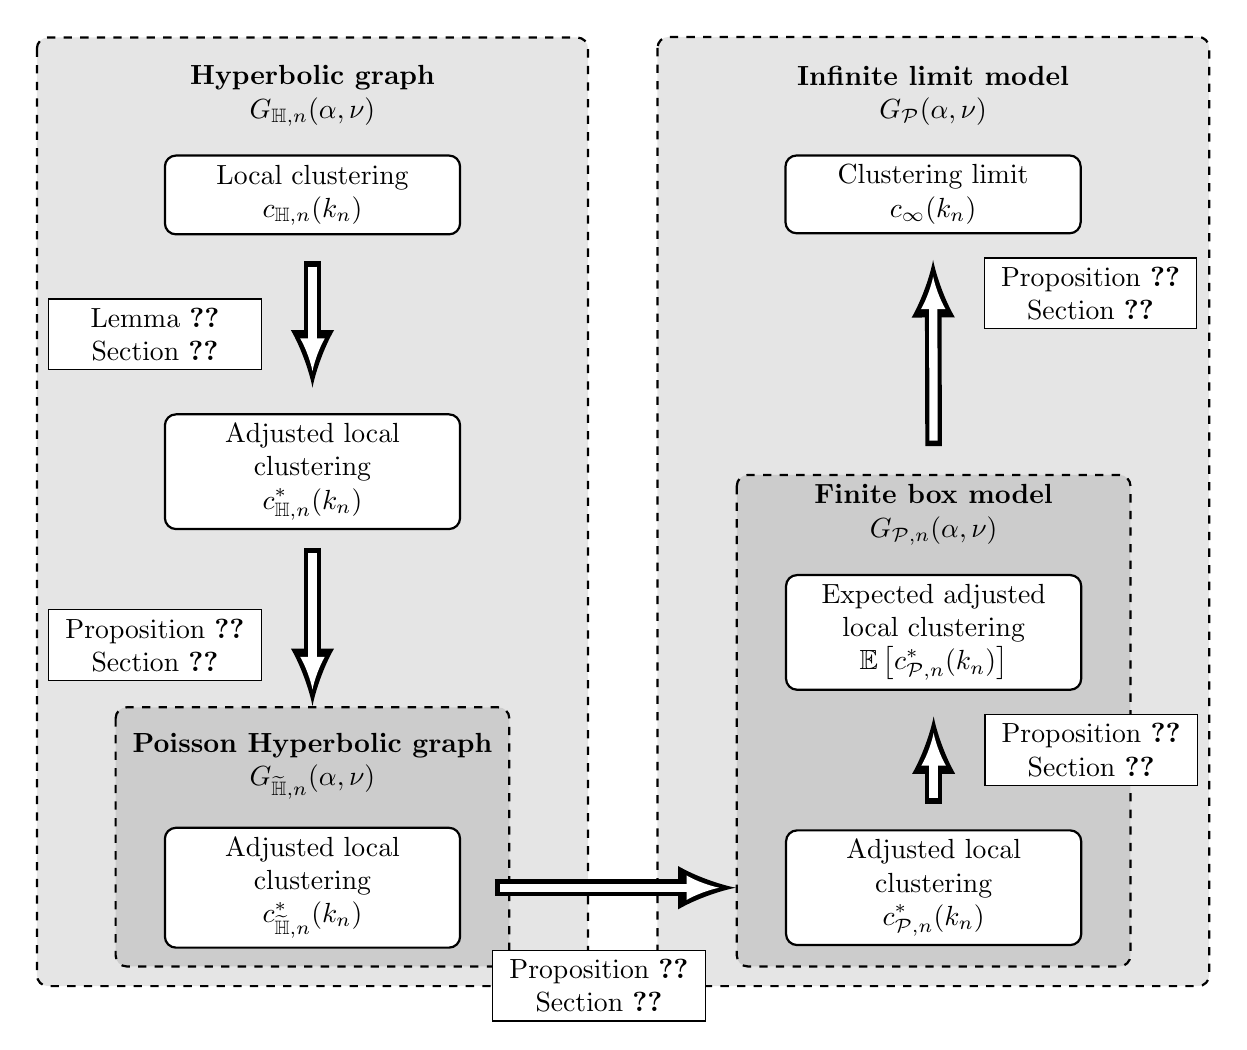
\begin{tikzpicture}

\pgfdeclarelayer{background}
\pgfdeclarelayer{foreground}
\pgfsetlayers{background,main,foreground}

\tikzstyle{block} = [draw, text centered, rounded corners, draw=black, thick, fill=white]
\tikzstyle{textblock} = [draw, text centered, draw=black, fill=white]

\tikzset{
  double arrow/.style args={#1 colored by #2 and #3}{
    -latex,line width=#1,#2, % first arrow
    postaction={draw,-latex,#3,line width=(#1)/2,
                shorten <=(#1)/3,shorten >=(#1)}, % second arrow
  }
}

\draw node (anchor) at (0,0) {};

%Hyperbolic graph: top left

\path (anchor)+(0,0) node (hyp_header) {\begin{minipage}[c]{10em}
	\begin{center}
		\textbf{Hyperbolic graph}\\
		$G_{\H,n}(\alpha, \nu)$
	\end{center}
\end{minipage}};

\path (hyp_header.south)+(0,-0.75) node (c_hyp) [block] {\begin{minipage}[c]{10em}
	\begin{center}
	Local clustering\\
	$\displaystyle c_{\H,n}(k_n)$
	\end{center}
\end{minipage}};






%Adjusted local clustering: middle left

\path (c_hyp.south)+(0,-3) node (c_ast_hyp) [block] {\begin{minipage}[c]{10em}
	\begin{center}
	Adjusted local clustering\\
	$\displaystyle c_{\H,n}^\ast(k_n)$
	\end{center}
\end{minipage}};

\path (c_ast_hyp.north)+(-2,1) node (hyp_text) [textblock] {\begin{minipage}[c]{7em}
	\begin{center}
		Lemma \ref{lem:clustering_ast_H}\\
		Section~\ref{ssec:coupling_H_HP}
	\end{center}
\end{minipage}};

%Poisson Hyperbolic graph: middle left

%\path (c_hyp.south)+(0,-6) node (c_pois_hyp) [block] {\begin{minipage}[c]{12em}
%	\begin{center}
%	Local clustering\\
%	$\displaystyle c_{\widetilde{\H},n}(k_n)$
%	\end{center}
%\end{minipage}};



\path (c_ast_hyp.south)+(0,-3) node (pois_hyp_header) {\begin{minipage}[c]{13em}
	\begin{center}
		\textbf{Poisson Hyperbolic graph}\\
		$G_{\HP,n}(\alpha,\nu)$
	\end{center}
\end{minipage}};

\path (pois_hyp_header.north)+(-2,1) node (pois_hyp_text) [textblock] {\begin{minipage}[c]{7em}
	\begin{center}
		Proposition \ref{prop:clustering_ast_H_Pois}\\
		Section~\ref{ssec:coupling_H_HP}
	\end{center}
\end{minipage}};





%Poisson Hyperbolic graph: bottom left

\path (pois_hyp_header.south)+(0,-1) node (c_ast_pois_hyp) [block] {\begin{minipage}[c]{10em}
	\begin{center}
	Adjusted local clustering\\
	$\displaystyle c_{\HP,n}^\ast(k_n)$
	\end{center}
\end{minipage}};



%Infinite limit model: top right



\path (hyp_header.east)+(6,0) node (pois_header) {\begin{minipage}[c]{10em}
	\begin{center}
		\textbf{Infinite limit model}\\
		$G_{\Pcal}(\alpha, \nu)$
	\end{center}
\end{minipage}};

\path (pois_header)+(0,-1.25) node (c_infty) [block] {\begin{minipage}[c]{10em}
	\begin{center}
	Clustering limit\\
	$\displaystyle c_\infty(k_n)$
	\end{center}
\end{minipage}};

\path (c_infty.south)+(2,-0.75) node (exp_c_pois_text) [textblock] {\begin{minipage}[c]{7em}
	\begin{center}
		Proposition \ref{prop:convergence_average_clustering_P_n}\\
		Section \ref{sec:clustering_Pn_to_P}
	\end{center}
\end{minipage}};




%Finite box model: bottom right

\path (c_ast_pois_hyp.east)+(6,0) node (c_ast_pois_n) [block] {\begin{minipage}[c]{10em}
	\begin{center}
	Adjusted local clustering\\
	$\displaystyle c_{\Pcal,n}^\ast(k_n)$
	\end{center}
\end{minipage}};

\path (c_ast_pois_n.south)+(-4.25,-0.5) node (c_ast_pois_n_text) [textblock] {\begin{minipage}[c]{7em}
	\begin{center}
		Proposition \ref{prop:couling_c_H_P}\\
		Section \ref{ssec:coupling_HP_ast_P}
	\end{center}
\end{minipage}};

\path (c_ast_pois_n.north)+(0,2.5) node (exp_c_pois_n) [block] {\begin{minipage}[c]{10em}
	\begin{center}
	Expected adjusted local clustering\\
	$\displaystyle \Exp{c_{\Pcal,n}^\ast(k_n)}$
	\end{center}
\end{minipage}};

\path (exp_c_pois_n.south)+(2,-0.75) node (exp_c_pois_n_text) [textblock] {\begin{minipage}[c]{7em}
	\begin{center}
		Proposition \ref{prop:concentration_local_clustering_P_n}\\
		Section \ref{sec:concentration_c_P_n}
	\end{center}
\end{minipage}};

\path (exp_c_pois_n.north)+(0,0.75) node (pois_n_header) {\begin{minipage}[c]{13em}
	\begin{center}
		\textbf{Finite box model}\\
		$G_{\Pcal,n}(\alpha, \nu)$
	\end{center}
\end{minipage}};








%Arrows

\path (c_hyp.south)+(0,-0.2) node (arrow_1l) {};
\path (c_ast_hyp.north)+(0,0.2) node (arrow_1r) {};

\draw [double arrow=6pt colored by black and white] (arrow_1l) -- (arrow_1r);

\path (c_ast_hyp.south)+(0,-0.1) node (arrow_2l) {};
\path (pois_hyp_header.north)+(0,0.1) node (arrow_2r) {};

\draw [double arrow=6pt colored by black and white] (arrow_2l) -- (arrow_2r);

\path (c_ast_pois_hyp.east)+(0.3,0) node (arrow_3l) {};
\path (c_ast_pois_n.west)+(-0.5,0) node (arrow_3r) {};

\draw [double arrow=6pt colored by black and white] (arrow_3l) -- (arrow_3r);

\path (c_ast_pois_n.north)+(0,0.2) node (arrow_4l) {};
\path (exp_c_pois_n.south)+(0,-0.2) node (arrow_4r) {};

\draw [double arrow=6pt colored by black and white] (arrow_4l) -- (arrow_4r);

\path (exp_c_pois_n.north)+(0,1.5) node (arrow_5l) {};
\path (c_infty.south)+(0,-0.2) node (arrow_5r) {};

\draw [double arrow=6pt colored by black and white] (arrow_5l) -- (arrow_5r);

\begin{pgfonlayer}{background}

\path (c_hyp)+(-3.5,2) node (hyp_a) {};
\path (c_ast_pois_hyp)+(3.5,-1.25) node (hyp_b) {};
\path[rounded corners, draw=black, dashed, thick, fill=black!10] (hyp_a) rectangle (hyp_b);

\path (pois_hyp_header)+(-2.5,0.75) node (pois_hyp_a) {};
\path (c_ast_pois_hyp)+(2.5,-1) node (pois_hyp_b) {};
\path[rounded corners, draw=black, dashed, thick, fill=black!20] (pois_hyp_a) rectangle (pois_hyp_b);

\path (c_infty)+(-3.5,2) node (pois_a) {};
\path (c_ast_pois_n)+(3.5,-1.25) node (pois_b) {};
\path[rounded corners, draw=black, dashed, thick, fill=black!10] (pois_a) rectangle (pois_b);

\path (exp_c_pois_n)+(-2.5,2) node (pois_n_a) {};
\path (c_ast_pois_n)+(2.5,-1) node (pois_n_b) {};
\path[rounded corners, draw=black, dashed, thick, fill=black!20] (pois_n_a) rectangle (pois_n_b);

\end{pgfonlayer}

\end{tikzpicture}

\caption{Overview of the proof strategy for Theorem \ref{thm:local_clustering_hyperbolic}.}
\label{fig:overview_proof}
\end{figure}


\subsection{Adjusted clustering and Poisson nodes in hyperbolic graphs}

Recall that the first step for the fixed $k$ case was to show that the transition from the hyperbolic random graph $G_{\H,n}$ to the Poisson version $G_{\HP,n}$ did not influence clustering. Here we first make a transition from the local clustering function $c_{\H,n}(k)$ to the adjusted version $c_{\H,n}^\ast(k)$. The following lemma justifies working with this modified version. The proof uses a concentration result for $\N_{\H,n}(k_n)$ and full details can be found in Section~\ref{ssec:coupling_H_HP}.

\begin{lemma}\label{lem:clustering_ast_H}
As $n \to \infty$,
\[
	\Exp{\left|c_{\H,n}(k_n) - c_{\H,n}^\ast(k_n)\right|} = \smallO{s_\alpha(k_n)}.
\]
\end{lemma}

We then establish that the modified local clustering function in the hyperbolic model $G_{\H,n}(\alpha,\nu)$ behaves similarly to that in the Poisson version $G_{\HP, n}(\alpha,\nu)$. This is based on a standard coupling between a Binomial Point Process and Poisson Point Process.

\begin{proposition}\label{prop:clustering_ast_H_Pois}
As $n \to \infty$,
\[
	\Exp{\left|c_{\H,n}^\ast(k_n) - c_{\HP,n}^\ast(k_n)\right|} = \smallO{s_\alpha(k_n)}.
\]
\end{proposition}
%\MS{I think we can drop the condition to be increasing here and below, also the $n^{1/3}$ should be removed.}

\subsection{Coupling of local clustering between $G_{\HP,n}$ and $G_{\Pcal,n}$}

The next step is to show that the modified clustering is preserved under the coupling described in Section~\ref{ssec:coupling_H_P}. The proof can be found in Section~\ref{ssec:coupling_HP_ast_P}. This is one of the key technical challenges we face. 

To understand why, recall that the degree $k$ of a node is related to its height $y$, roughly speaking, by $k \approx \xi_{\alpha, \nu} e^{y/2}$. Therefore, when $k$ is fixed we have that the heights of nodes with that degree are also fixed, in particular $y < R_n/4$ for large enough $n$. In addition, the main contribution of triangles would also come from nodes with heights $y^\prime < R_n/4$. This allowed us to use Lemma~\ref{lem:coupling_edges} and conclude that the triangles present in the graph $G_{\HP,n}$ where exactly those present in $G_{\Pcal,n}$ and therefore the local clustering function was the same in both models. When $k_n \to \infty$ this is no longer true in general. For instance, suppose $k_n = n^{\frac{1-\varepsilon}{2\alpha + 1}}$, for some small $0 < \varepsilon < 1$. Then the relation $k_n \approx \xi_{\alpha, \nu} e^{y_n/2}$ implies that $y_n \approx \frac{2(1-\varepsilon)}{2\alpha + 1}\log(n) - 2\log(\xi_{\alpha, \nu})$. Since
$R_n/4 = \frac{1}{2}\log(n) - \frac{1}{2}\log(\nu)$ we get that $R_n/4 = \smallO{y_n}$ for all $\alpha > (3 - 4\varepsilon)/2$ and hence $y_n > R_n/4$ for large enough $n$, violating the conditions of Lemma~\ref{lem:coupling_edges}. However, by carefully analyzing the difference between the adjusted local clustering function in both models we can still make the same conclusion. This is summarized in the following proposition whose proof is found in Section~\ref{ssec:coupling_HP_ast_P}.

\begin{proposition}[Coupling result for local clustering]\label{prop:couling_c_H_P}
As $n \to \infty$,
\[
	\Exp{\left|c_{\HP,n}^\ast(k_n) - c_{\Pcal,n}^\ast(k_n)\right|} = \smallO{s_\alpha(k_n)}.
\]
\end{proposition}

\TM{ Maybe we could replace these three with a statement on $|c_{\H,n}(k_n) - c_{\Pcal,n}^\ast(k_n)|$, at least at this point of the paper. This is only the high level description and that is all we need for the ``final proof".}\PvdH{I would vote for keeping them split, since this allows us to clearly point to the main technical challenge we have to overcome to obtain the final result.}
These three results together imply that the difference between the local clustering function of the hyperbolic random graph and the modified local clustering function of the finite box graph converges to zero faster than the proposed scaling $s_\alpha(k_n)$ in Theorem [??]. Hence, to prove this theorem it is enough to prove it for $c_{\mathcal{P},n}^\ast(k)$. 

\subsection{From the finite to the infinite model}

To compute the limit of the modified local clustering function $c_{\mathcal{P},n}^\ast(k)$ in the finite graph $G_{\mathcal{P},n}(\alpha, \nu)$ we first prove in Section~\ref{sec:concentration_c_P_n} that it is concentrated around its expectation $\Exp{c_{\mathcal{P},n}^\ast(k_n)}$.

\TM{ ``concentration'' is a loaded term in probability. I am not sure this use of the word will not be counterintuitive to many. }\PvdH{I am not sure. Concentration generally refers to how much a random variable deviates from its expectation. This is exactly what this proposition tells us. I would therefore vote for keeping this terminology, although I would have no problem with replacing it with an other term if someone has a good suggestion.}

\begin{proposition}[Concentration for local clustering function in $G_{\mathcal{P},n}(\alpha, \nu)$]\label{prop:concentration_local_clustering_P_n}
As $n \to \infty$,
\[
	\Exp{\left|c_{\mathcal{P},n}^\ast(k_n) - \Exp{c_{\mathcal{P},n}^\ast(k_n)}\right|} = \smallO{s_\alpha(k_n)}.
\]
\end{proposition}

This result is another one of the technical challenges we face when considering $k_n \to \infty$. For the proof, we first identify the specific range of heights that give the main contribution to the triangle count, showing that the triangles coming from nodes with heights outside this range is of smaller order. Then we prove a concentration result for the main term, by carefully analyzing the joint neighborhoods of two nodes whose heights fall into the identified range. The full details are found in Section~\ref{sec:concentration_c_P_n}.

Assuming this concentration result, we are left with the task to compute the limit of $\Exp{c_{\mathcal{P},n}^\ast(k_n)}$ as $n \to \infty$ and show that it is equivalent to $c_\infty(k_n)$. To accomplish this we move to the infinite limit model $G_\Pcal(\alpha,\nu)$ and show that the difference between the expected value of the clustering function $c_G^\ast(k)$ in $G_{\mathcal{P},n}(\alpha,\nu)$ and $G_{\mathcal{P}}(\alpha,\nu)$ goes to zero faster than the proposed scaling in Theorem \ref{thm:local_clustering_hyperbolic}.

\begin{proposition}[Transition to the infinite limit model]\label{prop:convergence_average_clustering_P_n}
As $n \to \infty$,
\[
	\left|\Exp{c_{\Pcal,n}^\ast(k_n)} - c_\Pcal(k_n)\right| = \smallO{s_\alpha(k_n)}.
\]
\end{proposition}

\TM{ This is only for $c(k)$. Should we not also mean $c$? }\PvdH{I do not think so. We can prove everything for $c$ once we have the result for $c(k_n)$.}

Recall that for the finite box model the left and right boundaries of $\Rcal_n$ where identified, so that graph $G_{\Pcal,n}$ contains some additional edge with respect to the induced subgraph of $G_{\Pcal}$ on $\Rcal_n$. The prove of Proposition~\ref{prop:convergence_average_clustering_P_n} therefore relies on analyzing the number of triangles coming from these additional edges and showing that their contribution to the local clustering function are of negligible order, see Section~\ref{sec:clustering_Pn_to_P}. 

\subsection{Proof of the main results}\label{ssec:proof_main_result_diverging_k}

We are now ready to prove Theorem [??], using the propositions stated in the previous sections. As mentioned before, we focus here on the convergence statements. The computation of the exact expressions is done in Section~\ref{sec:asymptotics_average_clustering_ast_P}. We begin with Theorem~\ref{thm:local_clustering_hyperbolic}.

\begin{proof}[Proof of Theorem \ref{thm:local_clustering_hyperbolic}]
%By applying Proposition~\ref{prop:convergence_average_clustering_P_n}, Proposition~\ref{prop:convergence_average_clustering_P_n} and Theorem~\ref{thm:asymptotics_average_clustering_P} we get
%\begin{align*}
%	&\hspace{-30pt}\Exp{\left|\frac{c_{\Pcal,n}^\ast(k_n)}{C_{\alpha,\nu}s_\alpha(k_n)} - 1\right|}\\
%	&\le \frac{\Exp{\left|c_{\Pcal,n}^\ast(k_n) - \Exp{}c_{\Pcal,n}^\ast(k_n)\right|}}{C_{\alpha,\nu}s_\alpha(k_n)}
%		+ \frac{\left|\Exp{c_{\Pcal,n}^\ast(k_n)} - c_\infty(k_n)\right|}{C_{\alpha,\nu}s_\alpha(k_n)}
%		+ \left|\frac{c_{\infty}(k_n)}{C_{\alpha,\nu}s_\alpha(k_n)} - 1\right| \\
%	&= \smallO{1}.
%\end{align*}
First of all, due to cancellation of equal terms we can rewrite
\begin{align*}
    c_{\H,n}(k_n)-c_\infty(k_n) =& c_{\H,n}(k_n)-c_{\H,n}^\ast(k_n)+c_{\H,n}^\ast(k_n)-c_{\HP,n}^\ast(k_n)+c_{\HP,n}^\ast(k_n)-c_{\Pcal,n}^\ast(k_n) \\
    &+c_{\Pcal,n}^\ast(k_n)-\E c_{\Pcal,n}^\ast(k_n)+\E c_{\Pcal,n}^\ast(k_n)-c_\infty(k_n)
\end{align*}
Then, we take absolute values and apply the triangle inequality. By monotonicity of expectation, we can apply it to both sides and obtain
\begin{align*}
    \E[|c_{\H,n}(k_n)-c_\infty(k_n)|] \leq & \E[|c_{\H,n}(k_n)-c_{\H,n}^\ast(k_n)|]+\E[|c_{\H,n}^\ast(k_n)-c_{\HP,n}^\ast(k_n)|]\\&+\E[|c_{\HP,n}^\ast(k_n)-c_{\Pcal,n}^\ast(k_n)|] 
    +\E[|c_{\Pcal,n}^\ast(k_n)-\E c_{\Pcal,n}^\ast(k_n)|]\\&+\E[|\E c_{\Pcal,n}^\ast(k_n)-c_\infty(k_n)|]
\end{align*}
At this point, the lemmas and propositions presented above in this section can be applied in order to show that all summands are $\smallO{s_\alpha(k_n)}$: Lemma~\ref{lem:clustering_ast_H} for the transition to the modified clustering function in the first term, Proposition~\ref{prop:clustering_ast_H_Pois} for the Poissonization in the disk in the second term, Proposition~\ref{prop:couling_c_H_P} for the coupling from the disk to the finite box model in the third term, Proposition~\ref{prop:concentration_local_clustering_P_n} for the concentration in the fourth term and finally Proposition~\ref{prop:convergence_average_clustering_P_n} for the transition to the infinite limit model where we also used that $c_{\Pcal}(k_n) = c_\infty(k_n)$ as obtained at the end of Section~\ref{sec:asymptotics_average_clustering_ast_P}.
\TM{ Maybe we can have a more clear reference? Now, at this place in the paper this proof feels a bit like cheating since there are almost no details given. } \PvdH{I completely agree. I think that once the results for fixed $k$ have been included we can include a specific statement at the end of Section~\ref{sec:asymptotics_average_clustering_ast_P} we can refer to.} All of this together yields that:
\begin{align*}
    \E[|c_{\H,n}(k_n)-c_\infty(k_n)|] = \smallO{s_\alpha(k_n)} = \smallO{c_\infty(k_n)}
\end{align*}
\TM{ Last equality seems to rely on Thm 1.3, which is not yet proven at this point. }\PvdH{We can fix this by proving the scaling of $c_\infty(k)$ in Section~\ref{sec:asymptotics_average_clustering_ast_P}.}
i.e. the statement of the theorem.
%\[
%	\Exp{\left|\frac{c_{\Pcal,n}^\ast(k_n)}{C_{\alpha,\nu}s_\alpha(k_n)} - 1\right|}
%	\le \left|\frac{c_{\infty}(k_n)}{C_{\alpha,\nu}s_\alpha(k_n)} - 1\right| 
%	+ \frac{\Exp{\left|c_{\Pcal,n}^\ast(k_n) - c_\infty(k_n)\right|}}{C_{\alpha,\nu}s_\alpha(k_n)} = \smallO{1}.
%\]

%Combining this with Proposition~\ref{prop:couling_c_H_P} yields
%\[
%	\Exp{\left|\frac{c_{\H,n}^\ast(k_n)}{C_{\alpha,\nu}s_\alpha(k_n)} - 1\right|}
%	\le \Exp{\left|\frac{c_{\Pcal,n}^\ast(k_n)}{C_{\alpha,\nu}s_\alpha(k_n)} - 1\right|} 
%	+ \frac{\Exp{\left|c_{\H,n}^\ast(k_n) - c_{\Pcal,n}^\ast(k_n)\right|}}{C_{\alpha,\nu}s_\alpha(k_n)} = \smallO{1}.
%\]
%and the result then follows by applying Lemma~\ref{lem:clustering_ast_H}. 
\end{proof}




\section{Concentration of heights for vertices with degree $k$}\label{sec:concentration_argument}

In the proof of Proposition~\ref{prop:asymp} we used a result that allowed us to restrict integration over $y$ to the interval $[a(k)^-, a(k)^+]$, with
\[
	a(k)^\pm = 2\log\left(\frac{1 \pm C \sqrt{k \log(k)}}{\xi} \vee 1\right).
\]
The reason for this was that the integrand included the function $\rho(y,k) = \Prob{\Po(\mu(y)) = k}$, where $\Po(\lambda)$ denotes a Poisson random variable with expectation $\lambda$ and $\mu(y) = \mu(B_\Pcal(y)) = \xi e^{y/2}$, and Poisson random variables are well concentrated around their mean, i.e. around those values of $y$ for which $\mu(y) \approx k$.

In the remainder of this paper we will often encounter integrands involving, for some $\mu_n(y)$, the function $\Prob{\Po(\mu_n(y)) = k}$. In these case we want to be able to restrict our integration around those heights $y$ for which $\mu_n(y) \approx k_n$. We will refer to as \emph{concentration of heights arguments}. In this section we establish such results. We start with a concentration of heights lemma for the infinite model $\Ginf$ (Lemma~\ref{lem:concentration_argument}) and explain in Remark~\ref{rmk:concentration_argument} how such a result will be used throughout the paper. To obtain similar results for the other two models we have to first analyze the expected number of nodes in a typical neighborhood in these models. We do in Sections~\ref{ssec:average_degree_HP_n} and~\ref{ssec:average_degree_P_n}. We conclude this section with a general result that allows us to extend the concentration lemma for the infinite model to the hyperbolic random graph and finite box model.

\subsection{Concentration of heights argument for the infinite model}

%Recall that $\rho(y, k)$ is the probability density function of a Poisson random variable with expectation $\mu_{\alpha, \nu}(B_\Pcal(y)) = \xie^{\frac{y}{2}}$. 
%We will consider two different types of sequences $\{k_n\}_{n \ge 1}$, those that are asymptotically bounded and those that diverge. We define
%\begin{equation}\label{eq:def_kappa_n}
%	\kappa_n := \begin{cases}
%		\log(n) &\mbox{if } k_n = \bigT{1},\\
%		\sqrt{k_n \log(k_n)} &\mbox{if } k_n = \omega(1).
%	\end{cases}
%\end{equation}
%\TM{ This is not a good definition. There are sequences that neither stay bounded nor tend to infinity, e.q.~odd values equal to 2 even values equal to $\log n$. How do you decide for a given $k_n$ which of the two cases you pick. To solve this we could either restrict to sequences that are either a) constant or b) tending to infinity; or we could make a cut-off at some specific, slow growing function such as $\log\log\log n$. }\PvdH{You are right, I overlooked this fact. I would opt to go with the setting where we consider only sequences that are either asymptotically bounded or tend to infinity. After the new proves are added we can see where we specify this.}
For any positive sequence $a_n \to \infty$ and $C > 0$ we define
\begin{equation}\label{eq:def_K_C_set}
	\Kcal_C(a_n) = \left\{y \in \R_+ : \frac{a_n - C \sqrt{a_n \log(a_n)}}{\xi} \vee 1 \le e^{\frac{y}{2}}
	\le \frac{a_n + C \sqrt{a_n \log(a_n)}}{\xi} \right\}.
\end{equation}
In addition we define
\begin{equation}\label{eq:def_K_C_n_set}
	\Kcal_{C,n}(a_n) := (-I_n, I_n] \times ((0,R_n] \cap \Kcal_{C}(a_n)),
\end{equation}
where $I_n := \frac{\pi}{2}e^{R_n/2}$. In addition, for a sequence $a_n \to \infty$, we shall often use the shorthand notation
\begin{equation}\label{eq:def_kappa_n}
	\kappa_n := \sqrt{a_n \log(a_n)}
\end{equation}


%Where we recall that $a \vee b = \max\{a,b\}$ and $a \wedge b = \min\{a,b\}$.

The next lemma states that for a large class of functions $h(y)$, to compute the integral 
\[
	\int_{0}^\infty \rho(y,k_n) h(y) e^{-\alpha y} \dd y
\]
%\TM{ This part is supposed to be for the infinite model, yet you integrate over the finite box $\Rcal_n$. Is this really meant?
%I would have expected we just integrate wrt.~$y$ and replace $f_{\alpha,\nu}(x,y)$ by $\alpha e^{-\alpha y}$, the exponential density.}\PvdH{I understand this confusion and agree that your suggestion makes more sense here. However, I choose this setup to minimize notations later. I am for changing the setup to what you are suggesting but I will have to spend some time first on checking how that will effect the definitions in later sections.}
it is enough to consider integration over $\Kcal_C(k_n)$ instead of $\R_+$. More precisely, for any $\ell_n = (1 + \smallO{1})k_n$ it is enough to consider $\Kcal_C(\ell_n)$. The flexibility of using $(1+\smallO{1})k_n$ instead of $k_n$ will prove useful in later sections.

\begin{lemma}\label{lem:concentration_argument}
Let $\alpha > \frac{1}{2}$, $\nu > 0$, $\{k_n\}_{n \ge 1}$ be any positive sequence such that $k_n = o(n^{\frac{1}{2\alpha + 1}})$ and let $\ell_n = k_n(1 + \epsilon_n)$, with $\epsilon_n \to 0$. In addition let $\beta < \alpha$ and $h : \R_+ \rightarrow  \R$ be a any function such that $h(y) = g(y)e^{\beta y}$ with $|g(y)|$ uniformly bounded on $\R_+$. Then, if we define for $C > 0$
\[
	\lambda_n^\pm = (\ell_n \pm C \sqrt{\ell_n \log(\ell_n)}) \wedge \xi, 
	\quad a_n^\pm = 2 \log\left(\frac{\lambda_n^\pm}{\xi}\right),
\] 
%\TM{ If $k$ is constant, then $\ell^- < 0$ and hence 
%$a^-$ is undefined! Need to change the definitions. }\PvdH{You are right. I changed it by taking the minimum with $\xi$.}
we have
\begin{equation}\label{eq:error_bound_int_rho_not_K}
	\int_{\R_+ \setminus \Kcal_{C}(\ell_n)} \rho(y,k_n) h(y) \alpha e^{-\alpha y} \dd y
	= \bigO{k_n^{-(1+C^2)/2}}
\end{equation}
%\TM{ As before, this is not a proper dichotomy. (unless we assume more about the sequences $k_n$, i.e.~either constant or tending to infinity }
as $n \to \infty$. 

In particular, if $h_n(y)$ is a function such that $h_n(y) = \bigO{n^{-1} k_n^{s} e^{\beta y}}\rho(y,k_n)$ for some $s \in \R$ and $\beta < \alpha$ as $n \to \infty$. Then for $C > 0$ large enough we have
\[
	\lim_{n \to \infty} \int_{\Rcal_n \setminus \Kcal_{C,n}(\ell_n)} h_n(y) 
	f_{\alpha, \nu}(x,y) \dd x \dd y = 0,
\]
or equivalently,
\[
	\int_{\Rcal_n} \hspace{-5pt} h_n(y) f_{\alpha, \nu}(x,y) \dd x \dd y
	= (1+\smallO{1}) \int_{\Kcal_{C,n}(\ell_n)} \hspace{-5pt} h_n(y) f_{\alpha, \nu}(x,y) \dd x \dd y.
\]
\end{lemma}

\begin{proof}



Note that in this case we write
\[
	\kappa_n = \sqrt{\ell_n \log(\ell_n)}.
\]
and recall (see proof of Proposition~\ref{prop:asymp}) that $\rho(y,k_n)$, as a function of $y$, is strictly increasing on $[0,a_n^-]$ and strictly decreasing on $[a_n^+,\infty)$. Therefore, by our assumption on $h(y)$,
\begin{align*}
	&\hspace{-20pt}\int_{\R_+ \setminus [a_n^-, a_n^+]} h(y) \rho(y,k_n) 
		\alpha e^{-\alpha y} \dd y\\
    &= \bigO{1} \int_0^{a_n^-} e^{\beta y} \rho(y,k_n) \alpha e^{-\alpha y} \dd y 
    	+ \bigO{1}\int_{a_n^+}^{\infty} e^{\beta y} \rho(y,k_n) \alpha e^{-\alpha y}x \dd y \\
    &= \bigO{1} \int_0^{a_n^-} \rho(y,k_n) e^{-(\alpha-\beta) y} \dd y 
   		+ \bigO{1} \int_{a_n^+}^{\infty} \rho(y,k_n) e^{-(\alpha-\beta) y} \dd y\\
   	&\le \bigO{1}\rho(a_n^-,k_n)\int_0^{a_n^-} e^{-(\alpha-\beta) y} \, \dd y
   		+ \bigO{1} \rho(a_n^+,k_n) \int_{a_n^+}^{\infty} e^{-(\alpha-\beta) y} \, \dd y.
\end{align*}
Since $\alpha - \beta > 0$, we conclude that
\begin{equation}\label{eq:concentration_lemma_integral_bound}
	\int_{\R_+ \setminus [a_n^-, a_n^+]} h(y) \rho(y,k_n) \alpha e^{-\alpha y} \dd y
	= \bigO{1} \left(\rho(a_n^-,k_n) + \rho(a_n^+,k_n)\right) 
\end{equation}

We shall now bound the terms $\rho(a_n^\pm,k_n)$, starting with $\rho(a_n^+,k_n)$.  Using Stirling's approximation $k! \sim \sqrt{2\pi} k^{k + 1/2} e^{-k}$ as $k \to \infty$ we write
\begin{align*}
	\rho(a_n^+,k_n) &= \frac{\mu(a_n^+)^{k_n}}{k_n!} e^{-\mu(a_n^+)} \\
	&\sim (2\pi)^{-1/2} k_n^{-1/2} \left(\frac{\mu(a_n^+)}{k_n}\right)^{k_n} e^{-(\mu(a_n^+) - k_n)}\\
	&= (2\pi)^{-1/2} k_n^{-1/2} 
		e^{-k_n\left(\frac{\mu(a_n^+)}{k_n} - 1 - \log\left(\frac{\mu(a_n^+)}{k_n}\right)\right)}.
\end{align*}

Since 
\[
	\frac{\mu(a_n^+)}{k_n} = \frac{\lambda_n^{+}}{k_n} = 1 + \epsilon_n + C \frac{\kappa_n}{k_n} 
	= 1 + \epsilon_n + C \sqrt{\frac{(1+\epsilon_n)\log((1+\epsilon_n)k_n)}{k_n}},
\]
and $x - \log(1 + x) \sim x^2/2$ as $x \to 0$, we get 
\begin{align*}
	\rho(a_n^+,k_n) 
	&\le \sqrt{2\pi} k_n^{-1/2} 
		e^{-k_n\left(\epsilon_n + C \frac{\kappa_n}{k_n} - \log\left(1 + \epsilon_n + C \frac{\kappa_n}{k_n}\right)\right)}\\
	&\sim (2\pi)^{-1/2} k_n^{-1/2} e^{-\frac{k_n \left(\epsilon_n + C \kappa_n/k_n\right)^2}{2}} \\
	&= \bigO{k_n^{-(1+C^2)/2}},		\numberthis \label{eq:concentration_lemma_bound_an+}
\end{align*}
where for the last line we used that
\[
	-k_n \frac{\left(\epsilon_n + C \kappa_n/k_n\right)^2}{2} = -\frac{C^2}{2}\log(k_n) + \bigT{1}.
\]
A similar analysis as above yields
\begin{equation}\label{eq:concentration_lemma_bound_an-}
	\rho(a_n^-,k_n) \le \bigT{1} k_n^{-1/2} e^{-\frac{k_n \left(\epsilon_n - C \kappa_n/k_n\right)^2}{2}} = \bigO{k_n^{-(1+C^2)/2}}.
\end{equation} 


Plugging~\eqref{eq:concentration_lemma_bound_an-} and~\eqref{eq:concentration_lemma_bound_an+}  into~\eqref{eq:concentration_lemma_integral_bound} yields the result. The second statement immediately follows from the first by choosing a large enough $C$ and observing that
\[
	\int_{\Rcal_n \setminus \Kcal_{C,n}(\ell_n)} h_n(y) f_{\alpha,\nu}(x,y) \dd x \dd y
	\le n \int_{\R_+ \setminus [a_n^-, a_n^+]} h_n(y) \alpha e^{-\alpha y} \dd y.
\]
\end{proof}

\begin{remark}[Concentration of heights argument]\label{rmk:concentration_argument}
%\TM{ again, this is a loaded term. I would in the very least change to ``concentration of height'' everywhere }
Lemma~\ref{lem:concentration_argument} will prove very useful in the remainder of this paper since we often have to deal with integrands of the form $g_n(y) f_{\alpha,\nu}(x,y)$ where $g_n(y) = \bigO{n^{-1} k_n^{s}}e^{\beta y}\rho(y,k_n)$ for some $s \in \R$ and $\beta < \alpha$. In this case the lemma tells us that for a suitable $C > 0$ we only need to integrate over $\Kcal_C(k_n)$. In order words, we may always assume for $g_n(y)$ (for a penalty of $\smallO{1}$) that $k_n - C \kappa_n \le \xi e^{y/2} \le k_n + C \kappa_n$. We will refer to this as a \emph{concentration of heights argument}, e.g. \emph{by a concentration of heights argument}
\[
	\int_{\Rcal_n} g_n(y) \rho(y,k_n) f_{\alpha,\nu}(x,y) \dd x \dd y 
	= (1+\smallO{1}) n \int_{\Kcal_C(k_n)} g_n(y) \rho(y,k_n) \alpha e^{-\alpha y} \dd y.
\]
\PvdH{ @All:It might be a good idea to add one more example of how the concentration argument is used in the paper. I someone finds a good example we use later on, please add it here.}
\end{remark}

We will later establish similar results for the cases where we consider the hyperbolic and finite box model. Here we have to consider Poisson distributions with mean $\mu(\BallHyp{y})$ and $\mu(\BallPon{y})$, respectively. For this the following, slightly more general version of Lemma~\ref{lem:concentration_argument} will be important.

\begin{lemma}\label{lem:concentration_argument_rho_approximation}
Let $\alpha > \frac{1}{2}, \nu > 0$, $k_n$ be any positive sequence such that $k_n = o(n^{\frac{1}{2\alpha + 1}})$, $\ell_n = (1 + \epsilon_n)k_n$, with $\epsilon_n \to 0$ and let $\Kcal_{C,n}(\ell_n)$ be defined as in~\eqref{eq:def_K_C_n_set}. In addition, define $\hat{\rho}_n(y,k) = \Prob{\Po(\hat{\mu}_n(y)) = k}$, where $\hat{\mu}_n(y)$ satisfies, 
\[
	\hat{\mu}_n(y) = (1 + \phi_n(y))\mu(y),
\]
where $\phi_n(y)$ is a continuous differentiable function such that for some $0 < \varepsilon < 1$
\[
	\sup_{0 \le y \le (1 - \varepsilon)R_n} |\phi_n(y)| = 0.
\]
Then the following holds for some $C > 0$ large enough:
\begin{enumerate}
\item For any sequence of continuous functions $h_n(y) : \R_+ \to \R$ such that, uniformly on $(0,R_n]$, $h_n(y) = \bigO{k_n^s e^{\beta y} \hat{\rho}_n(y,k_n)}$, as $n \to \infty$, 
%\TM{ Why not adjust $h$ so that we incorporate $\hat\rho$ in line below. Then both items look more similar. }\PvdH{The reason for the bound on $h_n(y)$ in the first statement is that we want to use this for cases where $h_n(y) \le k_n^s \hat{\rho}_n(y,k_n)$ (see for instance the proof of Proposition~\ref{prop:convergence_average_clustering_P_n}.}  
for some $s < 2\alpha(2\alpha + 1)$ and $\beta < \alpha$, we have,
\[
	\int_{\Rcal_n} h_n(y) f_{\alpha,\nu}(x,y) \dd x \dd y 
	= (1 + o(1)) \int_{\Kcal_{C,n}(\ell_n)} h_n(y) f_{\alpha,\nu}(x,y) \dd x \dd y.
\]
\item For any continuous bounded function $h(y)$,
\[
	\int_{\Kcal_{C,n}(\ell_n)} h(y) \hat{\rho}_n(y,k_n) f_{\alpha,\nu}(x,y) \dd x \dd y
	= (1+\smallO{1}) n \int_{0}^\infty h(y) \rho(y,k_n) \alpha e^{-\alpha y} \dd y,
\]
as $n \to \infty$.
\end{enumerate}
\end{lemma}

\begin{proof}
Similarly to the proof of Lemma~\ref{lem:concentration_argument} we define 
\[
	\lambda_n^\pm = (\ell_n \pm C \kappa_n) \wedge \xi, \quad \text{and} \quad a_n^\pm = 2 \log\left(\frac{\lambda_n^\pm}{\xi}\right).
\] 
%\TM{ Same problem as in L3.1. $\lambda^-$ can be negative, in which case $a^-$ is undefined.}

In addition we fix $\varepsilon^\ast > 0$ such that $\varepsilon < \min\{1- \frac{s}{2\alpha(2\alpha + 1)},\varepsilon, 1\}$ and. Then since $h_n(y) = \hat{\rho}_n(y,k_n) \bigO{k_n^s}$ we have
\begin{align*}
	k_n^s \int_{(1-\varepsilon^\ast)R_n}^{R_n} \hat{\rho}_n(y,k_n) e^{-\alpha y} \dd y
	&= \bigO{1} \hat{\rho}_n((1-\varepsilon^\ast)R_n,k_n) k_n^s e^{-\alpha(1-\varepsilon^\ast)R_n} \\
	&= \bigO{\hat{\rho}_n((1-\varepsilon^\ast)R_n,k_n) k_n^s n^{-2\alpha(1 - \varepsilon^\ast)}} \\
	&= \smallO{ \hat{\rho}_n((1-\varepsilon^\ast)R_n,k_n) n^{\frac{s}{2\alpha + 1} - 2\alpha(1-\varepsilon^\ast)}} = \smallO{1},
\end{align*}
where the last step follows by our choice of $\varepsilon^\ast$. Hence it is enough to prove both statement on $\Rcal_n((1-\varepsilon)R_n, R_n)$ instead of $\Rcal_n$.
\PvdH{@All: This is where we use that $s < 2\alpha(2\alpha + 1)$. I think this can be removed by using a more careful bound but I am not sure this is needed.}

\paragraph{Proof of statement 1.}
Since we already showed that
\[
	\lim_{n \to \infty} k_n^s \int_{(1-\varepsilon)R_n}^{R_n} \hat{\rho}_n(y,k_n) e^{(\beta-\alpha) y} \dd y = 0,
\]
by our assumption on $h_n(y)$, it is enough to show that for sufficiently large $C > 0$,
\begin{equation}\label{eq:concentration_argument_an_-}
	\lim_{n \to \infty} k_n^s \int_0^{a_n^-} \hat{\rho}_n(y,k_n) e^{(\beta-\alpha) y} \dd y = 0,
\end{equation}
and
\begin{equation}\label{eq:concentration_argument_an_+}
	\lim_{n \to \infty} k_n^s \int_{a_n^+}^{(1-\varepsilon)R_n} \hat{\rho}_n(y,k_n) e^{(\beta-\alpha) y} \dd y = 0.
\end{equation}
%\TM{ Why can we change the upper limit of the integral? PLease elaborate (in the paper) }

For simplicity we write $\mu(y) := \mu_{\alpha,\nu}\left(\BallPo{y}\right)$.. Now fix some $0 < \delta < 1$ and let $n$ be large enough such that 
\begin{enumerate}
\item $\sup_{0 < y \le (1-\varepsilon)R_n} |\phi_n(y)| < \delta$,
\item $(\ell_n + C \kappa_n)(1 - \delta) > k_n$ and
\item $(\ell_n - C \kappa_n)(1 + \delta) < k_n$
\end{enumerate}

Next, recall that the function $\lambda \mapsto \Prob{\Po(\lambda) = k}$ is monotonic increasing on $[0,k]$ and monotonic decreasing on $[k, \infty)$. Then since for $n$ large enough we have 
\[
	\hat{\mu}_n(y) = \mu(y)(1 + \phi_n(y)) \ge \mu(y)(1 - \delta) \ge \mu(a_n^+)(1 - \delta)
	= (\ell_n + C \kappa_n)(1 - \delta) > k_n,
\]
it follows that 
\[
	\hat{\rho}_n(y,k_n) = \Prob{\Po(\hat{\mu}_n(y)) = k_n} \le \Prob{\Po(\mu(y)(1-\delta)) = k_n},
\]
for all $a_n^+ \le y \le (1-\varepsilon)R_n$. By making the change of variables $z = \mu^{-1}(\mu(y)(1-\delta)) = y + 2 \log(1-\delta)$ we then get
\begin{align*}
	k_n^s \int_{a_n^+}^{(1-\varepsilon)R_n} \hat{\rho}_n(y,k_n) e^{(\beta - \alpha)y} \dd y
	&\le k_n^s \int_{a_n^+}^{(1-\varepsilon)R_n} \Prob{\Po(\mu(y)(1-\delta)) = k_n} 
		e^{(\beta-\alpha) y} \dd y\\
	&= k_n^s (1-\delta)^{\beta - \alpha} \int_{a_n^+ + 2\log(1-\delta)}^{(1-\varepsilon)R_n + 2\log(1-\delta)} 
		\Prob{\Po(\mu(z)) = k_n} e^{(\beta - \alpha)z} \dd z\\
	&\le k_n^s (1-\delta)^{\beta - \alpha} \int_{a_n^+}^{\infty} \rho(z,k_n) e^{(\beta - \alpha)z} \dd z.
\end{align*}
Since Lemma~\ref{lem:concentration_argument} implies that for large enough $C$,
\[
	\lim_{n \to \infty} k_n^s \int_{a_n^+}^{\infty} \rho(z,k_n) e^{(\beta - \alpha)z} \dd z = 0,
\]
we have proven~\eqref{eq:concentration_argument_an_+}.

The proof of~\eqref{eq:concentration_argument_an_-} follows the same line of reasoning. This time we use that for $0 \le y \le a_n^-$,
\[
	\hat{\mu}_n(y) \le \mu(y)(1 + \delta) \ge \mu(a_n^-)(1 + \delta)
		= (\ell_n - C \kappa_n)(1 + \delta) < k_n,
\]
so that 
\[
	\hat{\rho}_n(y,k_n) = \Prob{\Po(\hat{\mu}_n(y)) = k_n} \le \Prob{\Po(\mu(y)(1+\delta)) = k_n}.
\]
Making a similar change of variables $z = y + 2 \log(1+\delta)$ we then get
\begin{align*}
	k_n^s \int_0^{a_n^-} \hat{\rho}_n(y,k_n) e^{(\beta - \alpha)y} \dd y
	&= k_n^s \int_0^{a_n^-}\Prob{\Po(\mu(y)(1-\delta)) = k_n} 
		e^{(\beta-\alpha) y} \dd y\\
	&\le k_n^s (1+\delta)^{\beta - \alpha} \int_0^{a_n^- + 2\log(1+\delta)} 
		\rho(z,k_n) e^{(\beta - \alpha)z} \dd z,
\end{align*}
and~\eqref{eq:concentration_argument_an_-} follows by another application of Lemma~\ref{lem:concentration_argument}. 

\paragraph{Proof of statement 2.}

The proof of the second statement follows the same line of reasoning as above. First note that by Lemma~\ref{lem:concentration_argument} and the first statement, it is enough to show that
\[
	\int_{a_n^-}^{a_n^+} \hat{\rho}_n(y,k_n) h(y) e^{-\alpha y} \dd y
	= \left(1 + o(1)\right) \int_{a_n^-}^{a_n^+} \rho(z,k_n) h(z) e^{-\alpha z} \dd z.
\] 
or equivalently,
\[
	\int_{a_n^-}^{a_n^+} \rho(z,k_n) h(z) e^{-\alpha z} \dd z
	= \left(1 + o(1)\right)\int_{a_n^-}^{a_n^+} \hat{\rho}_n(y,k_n) h(y) e^{-\alpha y} \dd y.
\] 

Using the change of variable $z = \mu^{-1}(\hat{\mu}_n(y))$ and writing $\hat{a}_n^\pm = \hat{\mu}_n^{-1}(\mu(a_n^\pm))$, we get
\begin{align*}
	&\hspace{-30pt}\int_{a_n^-}^{a_n^+} \rho(z,k_n) h(z) e^{-\alpha z} \dd z \\
	&= \int_{a_n^-}^{a_n^+} \Prob{\Po(\mu(z)) = k_n} h(z) e^{-\alpha z} \dd z\\
	&= \int_{\hat{a}_n^-}^{\hat{a}_n^+} \Prob{\Po(\hat{\mu}_n(y)) = k_n} h(\mu^{-1}(\hat{\mu}_n(y))) e^{-\alpha \mu^{-1}(\hat{\mu}_n(y))} 
		\frac{\hat{\mu}_n^\prime(y)}{\mu^\prime(\mu^{-1}(\hat{\mu}_n(y)))} \dd y,
\end{align*}
where the fraction is the last line follows from the chain rule and the fact that $(\mu^{-1})^\prime(t) = (\mu^\prime(\mu^{-1}(t)))^{-1}$.

Now recall that $\hat{\mu}_n(y) = \mu(y)(1 + \phi_n(y))$, with $\phi_n(y)$ continuous and differentiable and satisfying
$\max_{0 \le y \le (1 - \varepsilon)R_n} |\phi_n(y)| \to 0$. It follows that $\max_{0 \le y \le (1 - \varepsilon)R_n} |\phi_n^\prime(y)| \to 0$ which then implies that $\hat{\mu}_n^\prime(y) = (1 + \smallO{1})\mu^\prime(y)$ as $n \to \infty$, uniformly on $(0,(1-\varepsilon)R_n)$. In particular this holds uniformly on $[a_n^-, a_n^+]$. Next we note that $\mu^\prime(y) = \mu(y)/2$ from which it follows that uniformly on $[a_n^-, a_n^+]$,
\[
	\frac{\hat{\mu}_n^\prime(y)}{\mu^\prime(\mu^{-1}(\hat{\mu}_n(y)))}
	= \frac{2\hat{\mu}_n^\prime(y)}{\hat{\mu}_n(y)}
	= \frac{(1 + \smallO{1})2\mu^\prime(y)}{(1 + \smallO{1})\mu(y)}
	= (1+\smallO{1})
\]
In addition, uniformly on $[0,(1-\varepsilon)R_n]$,
\[
	\mu^{-1}(\hat{\mu}_n(y)) = 2 \log(\hat{\mu}(y)/\xi) = 2 \log(\mu(y)/\xi) + 2 \log(1 + \smallO{1}) = y + \smallO{1}.
\]
Therefore, by assumption on $h(y)$,
\begin{align*}
	&\hspace{-30pt}\int_{a_n^-}^{a_n^+} \rho(z,k_n) h(z) e^{-\alpha z} \dd z \\
	&= (1 + \smallO{1})e^{-\alpha b_n}\int_{\hat{a}_n^-}^{\hat{a}_n^+} \Prob{\Po(\hat{\mu}_n(y)) = k_n} h(y + \smallO{1})  
		e^{-\alpha y} \dd y\\
	&= (1 + \smallO{1}) \int_{\hat{a}_n^-}^{\hat{a}_n^+} \Prob{\Po(\hat{\mu}_n(y)) = k_n} h(y)  
		e^{-\alpha y} \dd y \\
	&= (1 + \smallO{1}) \int_{a_n^-}^{a_n^+} \Prob{\Po(\hat{\mu}_n(y)) = k_n} h(y)  
			e^{-\alpha y} \dd y,
\end{align*}
which finishes the proof.
\end{proof}

\subsection{Expected number of points in balls in the hyperbolic random graph}\label{ssec:average_degree_HP_n}

\TM{  the term ``average degree" does not fit very well with what goes on in this section. We are considering the expected number of points in a ball, but not yet computing the average degree of the graph. }\PvdH{I agree and have changed the header.}
Recall that under the coupling between the hyperbolic random graph and the finite box model, for two points $p, p^\prime$ with $y + y^\prime < R_n$, $p^\prime \in \BallHyp{p}$ exactly when $|x-x^\prime|_{\pi e^{R_n/2}} \le \Phi(r,r^\prime)$. In this setting, the coupling lemma (Lemma~\ref{lem:asymptotics_Omega_hyperbolic}) gives that  
\[
	e^{\frac{1}{2}(y+y^\prime)} - K e^{\frac{3}{2}(y+y^\prime) - R_n} \leq \Phi(r, r^\prime) 
		\leq  e^{\frac{1}{2}(y+y^\prime)} + K e^{\frac{3}{2}(y+y^\prime) - R_n},
\]
for some constant $K$. %\TM{ Say what $K$ is and what the restrictions on $r, r'$ are. } 
This result enables us to determine the measure of a ball around a given point $p=(0,y)$ which will be fairly useful in our subsequent analysis. Recall that the hyperbolic ball $\BallHyp{p}$ is a subset of $\Rcal_n$ and not of the hyperbolic disc $\Dcal_{R_n}$, i.e. the balls $\BallHyp{p}$ "live" in the finite box and not the hyperbolic disc.

\begin{lemma}\label{lem:average_degree_hyperbolic}
Let $\eps \in (0, 1)$. Then for all $0 \le y \le (1 - \eps)R_n$
\[
	 1 - \phi_{\H,n}^{(1)}(y) - \phi_{\H,n}^{(2)}(y) \le \frac{\Mu{\BallHyp{0,y}}}{\Mu{\BallPo{0,y}}} 
	 \le 1 - \phi_{\H,n}^{(1)}(y) + \phi_{\H,n}^{(2)}(y),
\]
where
\[
	\phi_{\H,n}^{(1)}(y) = \frac{2\alpha - 1 - 4\pi}{4\pi} e^{-(\alpha - \frac{1}{2})(R_n - y)} 
		+ \left(\alpha - \frac{1}{2}\right)\pi e^{-(\alpha - \frac{1}{2})R_n - y/2},
\]
and
\[
	\phi_{\H,n}^{(2)}(y) = 
	+ \begin{cases}
			\frac{(2\alpha - 1)K}{3 - 2\alpha}\left(e^{-(\alpha - \frac{1}{2})(R_n - y)} - e^{-(R_n - y)}\right)
			&\mbox{if } 1/2 < \alpha < 3/2,\\
			\frac{(2\alpha -1)K}{2} (R_n - y)e^{-(R_n - y)} &\mbox{if } \alpha = 3/2,\\
			\frac{(2\alpha - 1)K}{2\alpha - 3} \left(e^{-(R_n - y)} - e^{-(\alpha - \frac{1}{2})(R_n - y)}\right)
			&\mbox{if } \alpha > 3/2,
		\end{cases}
\]
with $K$ being the constant coming from the approximation of $\Phi$ in Lemma~\ref{lem:asymptotics_Omega_hyperbolic}.
%\TM{ We want to say in the lemma where $K$ comes from. (not everyone reads surrounding text, or reads linearly, in a paper as long as this one.) }
\end{lemma}

\begin{proof}
We perform the computation of $\Mu{\BallHyp{0,y}}$ by splitting the integration with respect to the height $y^\prime$ into the cases $y^\prime > R_n - y$ and $y^\prime \le R_n - y$, %\TM{ You have not said what $y^\prime$ is! } 
where for the latter we utilize Lemma~\ref{lem:asymptotics_Omega_hyperbolic}. Recall that $\Mu{\BallPo{0,y}} = \xi e^{y/2}$ where $\xi = \frac{4\alpha\nu}{\pi(2\alpha - 1)}$.

Note that $\BallHyp{(0,y)} \cap \Rcal_n ([R_n - y, R_n])= \Rcal_n([R_n-y,R_n])$. 
Thus, 
\begin{align*}
	&\hspace{-30pt}\Mu{\BallHyp{(0,y)} \cap \Rcal_n ([R_n - y, R_n])} \\
	&= \int_{R_n - y}^{R_n} \int_{I_n} f_{\alpha,\nu}(x^\prime, y^\prime) \dd x^\prime \dd y^\prime
		= \nu \alpha e^{R_n/2}\left(e^{-\alpha(R_n - y)} - e^{-\alpha R_n}\right)\\
	&= \Mu{\BallPo{0,y}} \frac{2\alpha - 1}{4\pi} \left( e^{-(\alpha - \frac{1}{2})(R_n - y)}
		- e^{-(\alpha - \frac{1}{2})R_n - y/2}\right) \numberthis \label{eq:mu_hyperbolic_ball_part_1}
\end{align*}


Next we will establish upper and lower bounds on $\Mu{\BallHyp{(0,y)} \cap\Rcal_n[(0,R_n-y)]}$. Using Lemma~\ref{lem:asymptotics_Omega_hyperbolic} we have 
\begin{align*}
	\Mu{\BallHyp{(0,y)} \cap\Rcal_n[(0,R_n-y)]} 
	&\le \frac{2\nu \alpha}{\pi} \int_{0}^{R_n - y} \left(e^{\frac{y + y^\prime}{2}} + K e^{\frac{3}{2}(y + y^\prime) - R_n}\right)
		e^{-\alpha y^\prime} \dd y^\prime\\
	&= \Mu{\BallPo{0,y}}\left(1 - e^{-(\alpha - \frac{1}{2})(R_n - y)}\right) \\
	&\hspace{10pt}+ \frac{2\nu \alpha}{\pi} K e^{\frac{3 y}{2} - R_n}\int_0^{R_n-y} e^{(\frac{3}{2} - \alpha)y^\prime} \dd y^\prime
\end{align*}
The last integral depends on the value of $\alpha$,
\[
	\int_0^{R_n-y} e^{(\frac{3}{2} - \alpha)y^\prime} \dd y^\prime
	= \begin{cases}
		\frac{2}{3 - 2\alpha}\left(e^{(\frac{3}{2} - \alpha)(R_n - y)} - 1\right) &\mbox{if } 1/2 < \alpha < 3/2,\\
		R_n - y &\mbox{if } \alpha = 3/2,\\
		\frac{2}{2\alpha-3}\left(1 - e^{-(\alpha - \frac{3}{2})(R_n - y)}\right) &\mbox{if } \alpha > 3/2.
	\end{cases}
\]
Therefore we get
\begin{align*}
	&\hspace{-30pt}\frac{2\nu \alpha}{\pi} K e^{\frac{3 y}{2} - R_n}
		\int_0^{R_n-y} e^{(\frac{3}{2} - \alpha)y^\prime} \dd y^\prime\\
	&= \Mu{\BallPo{0,y}}\begin{cases}
		\frac{(2\alpha - 1)K}{3 - 2\alpha}\left(e^{-(\alpha - \frac{1}{2})(R_n - y)} - e^{-(R_n - y)}\right)
		&\mbox{if } 1/2 < \alpha < 3/2,\\
		\frac{(2\alpha -1)K}{2} (R_n - y)e^{-(R_n - y)} &\mbox{if } \alpha = 3/2,\\
		\frac{(2\alpha - 1)K}{2\alpha - 3} \left(e^{-(R_n - y)} - e^{-(\alpha - \frac{1}{2})(R_n - y)}\right)
		&\mbox{if } \alpha > 3/2.
	\end{cases}\\
	&= \Mu{\BallPo{0,y}} \phi_{\H,n}^{(2)}(y)
\end{align*}
and hence
\[
	\Mu{\BallHyp{(0,y)} \cap\Rcal_n[(0,R_n-y)]} = \Mu{\BallPo{0,y}}\left(1 - e^{-(\alpha - \frac{1}{2})(R_n - y)} 
	+ \phi_{\H,n}^{(2)}(y)\right).
\]
Combining this with~\eqref{eq:mu_hyperbolic_ball_part_1} yields the required upper bound.

The lower bound follows by observing that the only difference with the above computations is the change of sign in front of 
\[
	\frac{2 \nu \alpha}{\pi} K e^{\frac{3 y}{2} - R_n}\int_0^{R_n-y} e^{(\frac{3}{2} - \alpha)y^\prime} \dd y^\prime.
\]
\end{proof}

\subsection{Expected number of points in balls in the finite box model}\label{ssec:average_degree_P_n}

%\TM{ same comment Re: average degree. }
For the finite box model $\Gbox$ we obtain a similar result for expected size of the balls.

\begin{lemma}\label{lem:average_degree_P_n}
For all $p \in \Rcal_n$, such that $y > 2\log(\pi/2)$,
\[
	\mu_{\alpha,\nu}(\BallPon{p}) = \mu_{\alpha,\nu}(\BallPo{p})\left(1 - \phi_n(y)\right)
\]
%\TM{ where did the curly B's go? }\PvdH{Typo. Fixed}
where $\phi_n(y) \ge 0$ is given by
\[
	\phi_n(y) = \left(\frac{\pi}{2}\right)^{-(2\alpha - 1)}e^{-(\alpha-\frac{1}{2})(R_n - y)}
	- \frac{(2\alpha - 1)\pi}{4\alpha}\left(\left(\frac{\pi}{2}\right)^{-2\alpha} 
	e^{-(\alpha - \frac{1}{2})(R_n - y)} - e^{-(\alpha - \frac{1}{2})R_n - \frac{y}{2}}\right).
\]
On the other hand, if $y \le 2 \log(\pi/2)$ then
\[
	\mu_{\alpha,\nu}(\BallPon{p}) = \mu_{\alpha,\nu}(\BallPo{p})\left(1 - e^{-(\alpha - \frac{1}{2})R_n}\right).
\]
\end{lemma}

\begin{proof}
First note that since we have identified the boundaries of $[-\frac{\pi}{2}e^{\frac{R_n}{2}}, \frac{\pi}{2}e^{\frac{R_n}{2}}]$ we can assume, without loss of generality, that $p = (0,y)$. We then have that the boundaries of $\BallPon{p}$ are given by the equations $x^\prime = \pm e^{\frac{y+y^\prime}{2}}$, which intersect the left and right boundaries of $[-\frac{\pi}{2}e^{\frac{R_n}{2}}, \frac{\pi}{2}e^{\frac{R_n}{2}}]$ at height
\[
	h(y) = R_n + 2 \log\left(\frac{\pi}{2}\right) - y.
\]
Therefore, if $y \le 2 \log(\pi/2)$ this intersection occurs above the height $R_n$ of the box $\Rcal_n$ while in the other case the full region of the box above $h(y)$ is connected to $p$. 

We will first consider the case where $y > 2 \log(\pi/2)$. Recall that $\mu_{\alpha,\nu}(\BallPo{p}) = \xi e^{\frac{y}{2}}$ where $\xi = \frac{4\alpha \nu}{(2\alpha - 1)\pi}$. Then, after some simple algebra, we have that
\begin{align*}
	\mu_{\alpha,\nu}(\BallPon{p})
	&= \int_0^{h(y)} \int_{-\frac{\pi}{2}e^{\frac{R_n}{2}}}^{\frac{\pi}{2}e^{\frac{R_n}{2}}} 
		\ind{|x^\prime| \le e^{\frac{y+y^\prime}{2}}} f_{\alpha,\nu}(x^\prime,y^\prime) \, dx^\prime \, dy^\prime\\
	&\hspace{10pt}+ \int_{h(y)}^{R_n} \int_{-\frac{\pi}{2}e^{\frac{R_n}{2}}}^{\frac{\pi}{2}e^{\frac{R_n}{2}}} 
		f_{\alpha,\nu}(x^\prime,y^\prime) \, dx^\prime \, dy^\prime\\
	&= \frac{2 \alpha \nu}{\pi} e^{\frac{y}{2}} \int_0^{h(y)} e^{-(\alpha - \frac{1}{2})y^\prime} \, dy^\prime
		+ \alpha \nu e^{\frac{R_n}{2}} \int_{h(y)}^{R_n} e^{-\alpha y^\prime} \, dy^\prime \\
	&= \xi e^{\frac{y}{2}}\left(1 - \left(\frac{\pi}{2}\right)^{-(2\alpha - 1)} 
		e^{-(\alpha - \frac{1}{2})(R_n - y)}\right)\\
	&\hspace{10pt}+ \nu e^{\frac{R_n}{2}}\left(\left(\frac{\pi}{2}\right)^{-2\alpha} e^{-\alpha(R_n - y)} 
		- e^{-\alpha R_n}\right)\\
	&= \mu_{\alpha,\nu}(\BallPo{p})\left(1 - \phi_n(y)\right).
\end{align*}
Since, for all $\alpha > \frac{1}{2}$,
\[
	\left(\frac{\pi}{2}\right)^{-(2\alpha - 1)} \ge \frac{(2\alpha - 1)\pi}{4\alpha} \left(\frac{\pi}{2}\right)^{-2\alpha}
\]
it follows that $\phi_n(y) \ge 0$.

When $y \le 2 \log(\pi/2)$ we have
\begin{align*}
	\mu_{\alpha,\nu}(\BallPon{p})
	&= \int_0^{R_n} \int_{-\frac{\pi}{2}e^{\frac{R_n}{2}}}^{\frac{\pi}{2}e^{\frac{R_n}{2}}} 
		\ind{|x^\prime| \le e^{\frac{y+y^\prime}{2}}} f_{\alpha,\nu}(x^\prime,y^\prime) \, dx^\prime \, dy^\prime\\
	&= \frac{2 \alpha \nu}{\pi} e^{\frac{y}{2}} \int_0^{R_n} e^{-(\alpha - \frac{1}{2})y^\prime} \, dy^\prime\\
	&= \mu_{\alpha,\nu}(\BallPo{p})\left(1 - e^{-(\alpha - \frac{1}{2})R_n}\right).
\end{align*}
\end{proof}

\subsection{Concentration of heights argument for hyperbolic and finite box model}

Let us define $\rho_{\Po}(y,k) = \Prob{\Po(\Mu{\BallHyp{y}}) = k}$ and $\rho_{\text{box}} = \Prob{\Po(\Mu{\BallPon{y}}) = k}$. Then since Lemma~\ref{lem:average_degree_P_n} implies that $\Mu{\BallHyp{(y)}}$ satisfies the requirements in Lemma~\ref{lem:concentration_argument_rho_approximation} while Lemma~\ref{lem:average_degree_hyperbolic} states that this holds for $\Mu{\BallPon{0,y}}$, we have the following important Corollary.

\begin{corollary}\label{cor:concentration_argument_other_models}
The statements of Lemma~\ref{lem:concentration_argument_rho_approximation} holds for the two distribution functions $\rho_{\Po}(y,k)$ and $\rho_{n}(y,k)$. 
\end{corollary}

%\begin{corollary}\label{cor:concentration_argument_other_models}
%Let $\hat{\rho}_n(y,k)$ be any of the two distribution functions $\rho_{\Po}(y,k)$ and $\rho_{n}(y,k)$ and let $\Kcal_{C,n}(\kappa_n)$ be defined as in~\eqref{eq:def_K_C_n_set}. Then, for any function $g_n(y)$ such that, uniformly on $(0, R_n]$, $g_n(y) = \bigO{k_n^{s} e^{\beta y}}$,
%%\TM{ Where did the $n^{-1}$ come from? Does not appear in L3.4. }\PvdH{I will elaborate on this once the statement of Lemma~\ref{lem:concentration_argument} is updated}, 
%as $n \to \infty$, for some $s < 2\alpha(2\alpha + 1)$ and $\beta < \alpha$,
%\[
%	\int_{\Rcal_n} g_n(y) \hat{\rho}_n(y,k_n) f_{\alpha,\nu}(x,y) \dd x \dd y
%	= (1+\smallO{1})n\int_{0}^\infty g_n(y) \rho(y,k_n) \alpha e^{-\alpha y} \dd y,
%\]
%for some $C > 0$ large enough.
%\end{corollary}

In particular we conclude that, similarly to the infinite limit model, concentration of heights arguments as described in Remark~\ref{rmk:concentration_argument} can be applied in the case of the hyperbolic random graphs and the finite box model.

\begin{remark}[Most frequent use of concentration of argument]
Note that it follows from Proposition~\ref{prop:asymp} that $P(y)$ satisfies the conditions in the both statements of Lemma~\ref{lem:concentration_argument_rho_approximation}. In particular, if $\hat{\rho}_n$ denote either $\rho_{\Po}$ or $\rho_{\text{box}}$, then as $n \to \infty$
\begin{equation}\label{eq:concentration_heights_argument_Py}
	\int_{\Rcal_n} P(y) \hat{\rho}_n(y,k_n) f_{\alpha,\nu}(x, y) \dd x \dd y
	= (1 + \smallO{1}) n \int_0^\infty P(y) \rho(y,k_n) \alpha e^{-\alpha y} \dd y.
\end{equation}
This is the form that will be use most frequently in the remainder of this paper.
\end{remark}




\section{From $G_{\mathcal{P}, n}(\alpha, \nu)$ to $G_{\mathcal{P}}(\alpha, \nu)$ (Proving Proposition \ref{prop:convergence_average_clustering_P_n})}\label{sec:clustering_Pn_to_P}

Now that we have a complete picture of the behavior of the local clustering coefficient and function in the limit model $G_\Pcal$ we will proceed to relate this to the clustering in the hyperbolic model $G_{\H,n}$. The first step is to relate the clustering in the infinite model to that of the finite box model $G_{\Pcal, n}$. Recall that $G_{\Pcal,n}$ is obtained by restricting the Poisson Point Process $\PPP$ to the box $\Rcal_n = (-I_n, I_n] \times (0, R_n]$, with $I_n = \frac{\pi}{2} e^{R_n/2}$ (we write $\Pcal_n$ for this process), and connecting two points $p_1, p_2 \in \Rcal_n$ if $|x_1 - x_2|_{\pi e^{R_n/2}} \le e^{(y_1 + y_2)/2}$. We recall that by definition of the norm $|.|_{\pi e^{R_n/2}}$ the left and right boundaries of $\Rcal_n$ are identified. See Section~\ref{ssec:finite_model} for more details. 
\TM{ This last bit of the sentence is already contained in the fact we us $|.|_{\pi e^{R_n/2}}$. To me it does not add anything, except possibly confusion. } \PvdH{I have updated this and just added a reminder of this.}

\begin{remark}[Diverging $k_n$]
Throughout this section $\{k_n\}_{n \ge 1}$ will denote an sequence of integers satisfying $k_n \to \infty$ and $k_n = \smallO{n^{\frac{1}{2\alpha + 1}}}$, as $n \to \infty$.
\end{remark}

In this section we shall compute the asymptotic difference between triangle counts in the finite and infinite model. First we recall the definition of $\Kcal_{C}(k_n)$
\[
	\Kcal_C(k_n) = \left\{p \in \Rcal : \frac{k_n - C \sqrt{k_n \log(k_n)}}{\xi_{\alpha,\nu}} \le e^{\frac{y}{2}}
	\le \frac{k_n + C \sqrt{k_n \log(k_n)}}{\xi_{\alpha,\nu}} \right\},	
\]
\TM{ Typo : $p\in\R$. Do you mean $\Rcal_n$? Or maybe 
$\R \times \R^+$? Still not sure that max and min in defn add anything. } \PvdH{It was a typo and is corrected. I have removed the max and min.}
%with
%\[
%	\kappa_n := \begin{cases}
%		\log(n) &\mbox{if } k_n = \bigT{1},\\
%		\sqrt{k_n \log(k_n)} &\mbox{else.}
%	\end{cases}
%\]
%\TM{ Same issue as before. }
In addition we note that the function $\phi_n(y)$ in Lemma~\ref{lem:average_degree_P_n} satisfies
\[
	\phi_n(y) = \bigT{e^{-(\alpha - \frac{1}{2})(R_n - y)}},
\]
as $R_n - y \to \infty$. Since $e^{y/2} = \bigT{k_n} = \smallO{e^{R_n}}$ as $n \to \infty$, uniformly on $\Kcal_C$, it follows that $\phi_n(y) = \bigT{k_n^{2\alpha - 1} n^{-(2\alpha - 1)}}$, uniformly on $\Kcal_C$. This yields the following useful corollary to Lemma~\ref{lem:average_degree_P_n}.

\begin{corollary}\label{cor:average_degree_P_n_K}
Let $\alpha > \frac{1}{2}$, $C > 0$. Then, for all $p \in \Kcal_{C}(k_n)$,
\[
	\mu_{\alpha,\nu ,n}(B_{\Pcal,n}(p)) = \mu_{\alpha,\nu}(B_\Pcal(p))\left(1 - \bigT{k_n^{2\alpha - 1} n^{-(2\alpha - 1)}}\right).
\]
\TM{ I don't follow. Spell it out. }\PvdH{I added additional explanation above. Please see if this solves the confusion.}

\end{corollary}


\subsection{Comparing triangles between $G_\Pcal(\alpha,\nu)$ and $G_{\Pcal,n}(\alpha,\nu)$}

We now turn to the task of calculating the expected number of triangles of a node at height $y$, for both the infinite model and the finite box model. Recall that we added a typical point $p_0 = (0,y)$, with exponentially distributed height, to the Poisson Point Process and that
\[
	\Exp{T_{\Pcal,n}(p_0)} = \frac{1}{2}\iint_{\Rcal_n^2} T_{\Pcal,n}(p_0,p_1,p_2)
	f_{\alpha,\nu}(x_1,y_1) f_{\alpha,\nu}(x_1,y_1) \, dx_1 \, dx_2 \, dy_1 \, dy_2,
\]
where
\[
	T_{\Pcal,n}(p_0,p_1,p_2) = \ind{p_1 \in B_{\Pcal,n}(p_0)}\ind{p_2 \in B_{\Pcal,n}(p_0)}\ind{p_2 \in B_{\Pcal,n}(p_1)}.
\]
\TM{ $p$ is supposed to be $p_0$ I assume. }\PvdH{Indeed. It has been corrected.}
The difference between the indicator $\ind{p_1 \in B_{\Pcal,n}(p)}$ in the finite box model and $\ind{p_1 \in B_{\Pcal}(p)}$ is that in $G_{\Pcal,n}(\alpha,\nu)$ we identified the boundaries of the interval $[-\frac{\pi}{2}e^{R_n/2}, \frac{\pi}{2} e^{R_n/2}]$ and we stop at height $y = R_n$. It is clear that for any $0 \le y \le R_n$ we have that $\BallPon{p_0} = \BallPo{p_0} \cap \Rcal_n$. However, when we take another point $p^\prime \in \BallPon{p}$ then it could happen that there are points in the intersection $\BallPon{p} \cap \BallPon{p^\prime}$ that are not in $\BallPo{p} \cap \BallPo{p^\prime}$. Let us denote this region by $\mathcal{T}_{\Pcal \Delta \Pcal_n}(p,p^\prime)$. Then, any $p_2 \in \mathcal{T}_{\Pcal \Delta \Pcal_n}(p,p^\prime)$ creates a triangle with $p$ and $p^\prime$ in $G_{\Pcal,n}(\alpha,\nu)$ that is not present in $G_{\Pcal}(\alpha, \nu)$.  

Define
\begin{equation}\label{eq:def_tilde_triangle_indicator}
	\widetilde{T}_{\Pcal,n}(p_0,p_1,p_2) = \ind{p_1 \in B_{\Pcal,n}(p_0)}\ind{p_2 \in B_{\Pcal,n}(p_0)}\ind{p_2 \in B_{\Pcal}(p_1) \cap \Rcal_n}
\end{equation}
Then
\[
	\sum_{p_1,p_2 \in \Pcal_n}^{\ne} T_{\Pcal,n}(p_0,p_1,p_2) - \widetilde{T}_{\Pcal,n}(p_0,p_1,p_2)
	= \sum_{p_1,p_2 \in \Pcal_n}^{\ne} \ind{p_1 \in \BallPon{p_0}} \ind{p_2 \in \mathcal{T}_{\Pcal \Delta \Pcal_n}(p_0,p_1)},
\]
\TM{ Note you cannot really force/assume $p_0 = (0,y)$ is in your PPP $\Pcal_n$. (The summation over $\Pcal_n \setminus (0,y)$ suggests this is what you do.) For taking the expectation of sort of thing, Palm theory / Mecke are used typically. At this point though you can again still just say we add $p_0$ to the PPP. }\PvdH{I changed the text at the beginning of this section to mention this. Since we now consider the point process $\Pcal_n \cup p_0$ the above summation is over $\Pcal_n$.}
where the sums are over all distinct pairs $(p_1, p_2) \in \Pcal_n$.

\begin{figure}[!t]
\centering
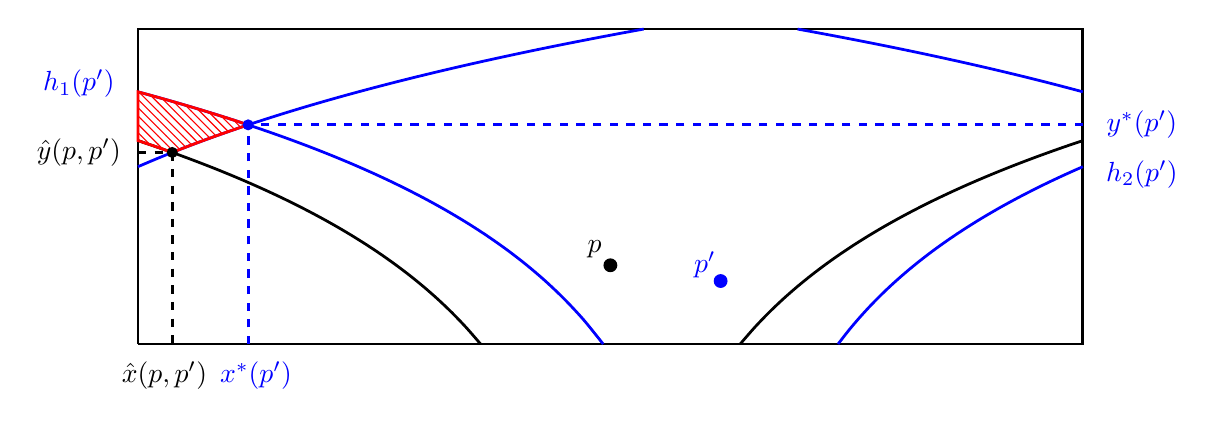
\begin{tikzpicture}
	%Define the coordinates 
	%p = (\u,\v) and p^\prime = (\uu, \vv)
	%Box \Rcal_n has width 2\r and height \t
	\pgfmathsetmacro{\u}{0} %0
	\pgfmathsetmacro{\v}{1} %1
	\pgfmathsetmacro{\uu}{1.4} %1.4
	\pgfmathsetmacro{\vv}{0.8} %0.8
	\pgfmathsetmacro{\r}{6}
	\pgfmathsetmacro{\t}{4}
	
	%The box \Rcal_n
	\draw[line width=1pt] (-\r,0) -- (\r,0) -- (\r,\t) -- (-\r,\t) -- (-\r,0);

	%Dram both nodes
    \draw node[fill, circle, inner sep=0pt, minimum size=5pt] (p1) at (\u,\v) {};
    \path (p1)+(-0.2,0.2) node {$p$};
    \draw node[fill,blue, circle, inner sep=0pt, minimum size=5pt] (p2) at (\uu,\vv) {};
    \path (p2)+(-0.2,0.2) node {\color{blue}$p^\prime$};
	
	
	%Boundaries p = (\u,\v)
	
	%Right boundary
	\pgfmathsetmacro{\rightbounduv}{\u+exp((\v)/2)}
	\draw[domain=\rightbounduv:\r,smooth,variable=\x,black,line width=1pt] plot (\x, {2*ln(\x)-\v});
    %Left boundary
    \pgfmathsetmacro{\leftbounduv}{\u-exp((\v)/2)}
    \draw[domain=\leftbounduv:-\r,smooth,variable=\x,black,line width=1pt] plot (\x, {2*ln(-\x)-\v});
    
    %Boundaries p^\prime = (\uu,\vv)
    
    %Right boundary
    \pgfmathsetmacro{\rightbounduuvv}{\uu+exp((\vv)/2)}
    \draw[domain=\rightbounduuvv:\r,smooth,variable=\x,blue,line width=1pt] plot (\x, {2*ln(\x-\uu)-\vv});
    %Shifted right boundary
    \pgfmathsetmacro{\shiftrightbounduuvv}{\uu+exp((\vv + \t)/2)-2*\r}
    \draw[domain=\shiftrightbounduuvv:-\r,smooth,variable=\x,blue,line width=1pt] plot (\x, {2*ln(\x+(2*\r-\uu))-\vv});
    %Left boundary 
    \pgfmathsetmacro{\leftbounduuvv}{\uu-exp((\vv)/2)}
    \draw[domain=\leftbounduuvv:-\r,smooth,variable=\x,blue,line width=1pt] plot (\x, {2*ln(\uu-\x)-\vv});
    %Shifted left boundary
    \pgfmathsetmacro{\shiftleftbounduuvv}{\uu-exp((\vv + \t)/2)+2*\r}
    \draw[domain=\shiftleftbounduuvv:\r,smooth,variable=\x,blue,line width=1pt] plot (\x, {2*ln(2*\r + \uu-\x)-\vv});
    
    %Define x^\ast(p^\prime) and y^\ast(p^\prime)
    \pgfmathsetmacro{\uuast}{\uu-\r}
    \pgfmathsetmacro{\vvast}{2*ln(\r)-\vv}
    
    %Define intersection left black and shifted blue curve
    \pgfmathsetmacro{\vast}{2*ln((2*\r - \uu)/(exp(\v/2) + exp(\vv/2)))}
    \pgfmathsetmacro{\uast}{(\uu - 2*\r)/(1 + exp((\vv - \v)/2))}    
   
    %Define h_1(p) = h_2(p)
    \pgfmathsetmacro{\hp}{2*ln(\r-\u)-\v}
    
    %Define h_1(p^\prime) and h_2(p^\prime)
    \pgfmathsetmacro{\hh}{2*ln(\uu+\r)-\vv}
    \pgfmathsetmacro{\hhh}{2*ln(\r-\uu)-\vv}
    
    %Highlight area between left black, left blue and shifted right blue line
	\draw[red,line width=1pt,pattern=north west lines, pattern color=red] 
		plot[domain=\uuast:\uast,smooth,variable=\x,red] (\x, {2*ln(\x+(2*\r-\uu))-\vv}) 
		-- 
		plot[domain=\uast:-\r,smooth,variable=\x,red] (\x, {2*ln(-\x)-\v})
		-- 
		(-\r,\hh)
		-- 
		plot[domain=-\r:\uuast,smooth,variable=\x,red] (\x, {2*ln(\uu-\x)-\vv});
	
%	\draw node[fill, circle, inner sep=0pt, minimum size=4pt, blue] at (\uuast,\vvast) {};
%	\draw node[fill, circle, inner sep=0pt, minimum size=4pt, black] at (\uast,\vast) {};
%	\draw node (f1) at (\uuast,\vvast+0.9) {\color{blue}$(x^\ast(p^\prime), y^\ast(p^\prime))$};
%	\draw node (f2) at (\uast+1,\vast-1.25) {\color{black}$(\hat{x}(p,p^\prime), \hat{y}(p,p^\prime))$};
%	
%	\draw[->,thick] (f2) -- (\uast+0.1,\vast-0.2);
%	\draw[->,thick,blue] (f1) -- (\uuast,\vvast+0.2);
	
	 \draw[dashed,line width=1pt,blue] (\uuast,0) -- (\uuast,\vvast);
	 \draw node at (\uuast+0.1,-0.4) {\color{blue}$x^\ast(p^\prime)$};
	 \draw[dashed,line width=1pt,blue] (\r,\vvast) -- (\uuast,\vvast);
	 \draw node at (\r+0.75,\vvast) {\color{blue}$y^\ast(p^\prime)$};
	 \draw[dashed,black,line width=1pt] (-\r,\vast) -- (\uast,\vast);
	 \draw node at (-\r-0.75,\vast) {\color{black}$\hat{y}(p,p^\prime)$};
	 \draw[dashed,black,line width=1pt] (\uast,\vast) -- (\uast,0);
	 \draw node at (\uast-0.1,-0.4) {\color{black}$\hat{x}(p,p^\prime)$};
	 
	 \draw node[fill, circle, inner sep=0pt, minimum size=4pt, blue] at (\uuast,\vvast) {};
	 \draw node[fill, circle, inner sep=0pt, minimum size=4pt, black] at (\uast,\vast) {};
	
    \draw node at (-\r-0.75,\hh+0.1) {\color{blue}$h_1(p^\prime)$};
    \draw node at (\r+0.75,\hhh-0.1) {\color{blue}$h_2(p^\prime)$};

\end{tikzpicture}
\caption{Example configuration of two points $p$ and $p^\prime$ for which $\BallPon{p} \cap \BallPon{p^\prime}$ is not a subset of $\BallPo{p} \cap \BallPo{p^\prime}$. The red region indicates the area of points belonging to $\BallPon{p} \cap \BallPon{p^\prime}$ but not to $\BallPo{p} \cap \BallPo{p^\prime}$.}
\label{fig:comparing_triangles_diff_intersections}
\end{figure}

Figure \ref{fig:comparing_triangles_diff_intersections} shows an example of a configuration where $\mathcal{T}_{\Pcal \Delta \Pcal_n}(p,p^\prime) \ne \emptyset$. We observe that $\mathcal{T}_{\Pcal \Delta \Pcal_n}(p,p^\prime) \ne \emptyset$ because the right boundary of the ball $\BallPon{p^\prime}$ exists the right boundary of the box $\Rcal_n$ and then, since we identified the boundaries, continues from the left so that $\BallPon{p^\prime}$ covers part of the ball $\BallPon{p}$ which would not be covered in the infinite limit model. 

To further analyze this, let us introduce some notation. For any $p = (x,y) \in \Rcal_n$ we will define the left and right boundary functions as, respectively,
\begin{align}
	b_p^-(z) &= \begin{cases}
		2 \log\left(x-z\right) - y &\mbox{if }  -\frac{\pi}{2} e^{R_n/2} \le z \le x - e^{y/2}  \\
		2\log\left(\pi e^{R_n/2} + x - z\right) - y 
			&\mbox{if } x - e^{(y + R_n)/2} + \pi e^{R_n/2} \le z \le \frac{\pi}{2} e^{R_n/2}\\
		0 &\mbox{else}
	\end{cases}\\
	b_p^+(z) &= \begin{cases}
		2 \log\left(z-x\right) - y &\mbox{if } x + e^{y/2} \le z \le \frac{\pi}{2} e^{R_n/2} \\
		2\log\left(\pi e^{R_n/2} + z - x\right) - y 
			&\mbox{if } -\frac{\pi}{2} e^{R_n/2} \le z \le x + e^{(y + R_n)/2} - \pi e^{R_n/2}\\
		0 &\mbox{else}
	\end{cases}
\end{align}
Note that these functions describe the boundaries of the ball $\BallPon{p}$. In particular, $p^\prime = \BL{(x^\prime, y^\prime)} \in \BallPon{p}$ if and only if $y^\prime \ge \min\left\{b_p^-(x^\prime), b_p^+(x^\prime)\right\}$.

Since we have identified the left and right boundary of $\Rcal_n$ we can assume, without loss of generality that $x = 0$. Due to symmetry it is then enough to restrict the analysis to the case where $x^\prime > 0$. \TM{ does this not depend on $p$? }\PvdH{I do not think so, because we can always take $p = (0,y)$ due to the invariance in the $x$-direction. I have updated the text to better reflect this.} 
There are two important points in the box $\Rcal_n$. These are the intersection between the left boundary of $p^\prime$ and the right boundary of $p^\prime$, as it continues from the left side of the box, and the left boundary of $p$. We denote by $(x^\ast(p^\prime), y^\ast(p^\prime))$ the intersection between the left and right boundary of $p^\prime$ and by $(\hat{x}(p,p^\prime), \hat{y}(p,p^\prime))$ the intersection between the left boundary of $p$ and the right boundary of $p^\prime$, see Figure \ref{fig:comparing_triangles_diff_analysis}. After some simple algebra \TM{ I am not a big fan of writing "after some simple algebra" or similar. This is how errors can creep into your argument. Maybe we can just give the details? } we obtain the following expressions for the coordinates of these two points
\begin{align*}
	x^\ast(p^\prime) &= x^\prime - \frac{\pi}{2} e^{R_n/2}\\
	y^\ast(p^\prime) &= 2\log\left(\frac{\pi}{2}e^{R_n/2}\right) - y^\prime\\
	\hat{x}(p,p^\prime) &= \frac{x^\prime - \pi e^{R_n/2}}{1 + e^{(y^\prime - y)/2}} \\
	\hat{y}(p,p^\prime) &= 2 \log\left(\frac{\pi e^{R_n/2} - x^\prime}{e^{y/2} + e^{y^\prime/2}}\right)
\end{align*}

The crucial observation is that $\mathcal{T}_{\Pcal \Delta \Pcal_n} = \emptyset$ as long as the point $(x^\ast(p^\prime), y^\ast(p^\prime))$ is above the left boundary of $p$. This happens exactly when $y^\ast(p^\prime) > b_p^-(x^\ast(p^\prime))$. Therefore the boundary of this event is given by the equation $y^\ast(p^\prime) = b_p^-(x^\ast(p^\prime))$ which reads
\[
	2\log\left(\frac{\pi}{2}e^{R_n/2}\right) - y^\prime = 2\log\left(\frac{\pi}{2} e^{R_n/2} -x^\prime\right) - y.
\]
Solving this equation gives us the function
\begin{equation}
	b^\ast_p(z) = y - 2\log\left(1 - \frac{z}{\frac{\pi}{2} e^{R_n/2}}\right),
\end{equation}
which is displayed by the red curve in Figure \ref{fig:comparing_triangles_diff_analysis}. It holds that $y^\ast(p^\prime) > b_p^-(x^\ast(p^\prime))$ if and only if $y^\prime < b^\ast_p(x^\prime)$ and hence we have that $\mathcal{T}_{\Pcal \Delta \Pcal_n} = \emptyset$ for all $p^\prime \in \Rcal_n$ for which $y^\prime \ge b^\ast_p(x^\prime)$. We also not that when $y^\prime = b^\ast_p(x^\prime)$ the two points $(x^\ast(p^\prime), y^\ast(p^\prime))$ and $(\hat{x}(p,p^\prime),\hat{y}(p,p^\prime))$ coincide.



\begin{figure}[!t]

\centering
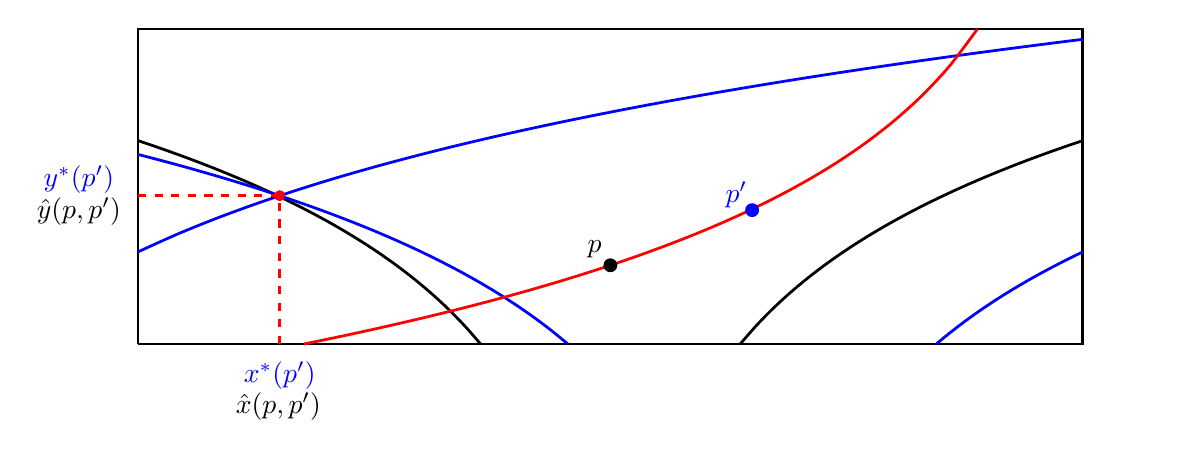
\begin{tikzpicture}
	%Define the coordinates 
	%p = (\u,\v) and p^\prime = (\uu, \vv)
	%Box \Rcal_n has width 2\r and height \t
	\pgfmathsetmacro{\u}{0}
	\pgfmathsetmacro{\v}{1}
	\pgfmathsetmacro{\uu}{1.8}
	\pgfmathsetmacro{\vv}{1.7}
	\pgfmathsetmacro{\r}{6}
	\pgfmathsetmacro{\t}{4}
	
	%The box \Rcal_n
	\draw[line width=1pt] (-\r,0) -- (\r,0) -- (\r,\t) -- (-\r,\t) -- (-\r,0);	
	
	%Boundaries p = (\u,\v)
	
	%Right boundary
	\pgfmathsetmacro{\rightbounduv}{\u+exp((\v)/2)}
	\draw[domain=\rightbounduv:\r,smooth,variable=\x,black,line width=1pt] plot (\x, {2*ln(\x)-\v});
    %Left boundary
    \pgfmathsetmacro{\leftbounduv}{\u-exp((\v)/2)}
    \draw[domain=\leftbounduv:-\r,smooth,variable=\x,black,line width=1pt] plot (\x, {2*ln(-\x)-\v});
    
    %Boundaries p^\prime = (\uu,\vv)
    
    %Right boundary
    \pgfmathsetmacro{\rightbounduuvv}{\uu+exp((\vv)/2)}
    \draw[domain=\rightbounduuvv:\r,smooth,variable=\x,blue,line width=1pt] plot (\x, {2*ln(\x-\uu)-\vv});
    %Shifted right boundary
    \pgfmathsetmacro{\shiftrightbounduuvv}{\uu+exp((\vv + \t)/2)-2*\r}
    %\draw[domain=\shiftrightbounduuvv:-\r,smooth,variable=\x,blue,line width=1pt] plot (\x, {2*ln(\x+(2*\r-\uu))-\vv});
    \draw[domain=-\r:\r,smooth,variable=\x,blue,line width=1pt] plot (\x, {2*ln(\x+(2*\r-\uu))-\vv});
    %Left boundary 
    \pgfmathsetmacro{\leftbounduuvv}{\uu-exp((\vv)/2)}
    \draw[domain=\leftbounduuvv:-\r,smooth,variable=\x,blue,line width=1pt] plot (\x, {2*ln(\uu-\x)-\vv});
    %Shifted left boundary

    
    %Star boundary
    \pgfmathsetmacro{\starleftbound}{\r*(1-exp(\v/2))}
    \pgfmathsetmacro{\starrightbound}{\r*(1-exp((\v-\t)/2))}
    \draw[domain=\starleftbound:\starrightbound,smooth,variable=\x,red, line width=1pt] plot (\x, {2*ln((\r/(\r-\x)))+\v});
    
    %Define h_1(p) = h_2(p)
    \pgfmathsetmacro{\hp}{2*ln(\r-\u)-\v}
%    \draw node at (\r+0.75,\hp) {\color{black}$h(y)$};
    \draw node at (\r+1,\hp) {};
    
    %Define h_1(p^\prime) and h_2(p^\prime)
    \pgfmathsetmacro{\hh}{2*ln(\uu+\r)-\vv}
    \pgfmathsetmacro{\hhh}{2*ln(\r-\uu)-\vv}

%    \draw node at (-\r-0.75,\hh+0.1) {\color{blue}$h_1(p^\prime)$};
%    \draw node at (\r+0.75,\hhh) {\color{blue}$h_2(p^\prime)$};
    
    %Define x^\ast(p^\prime) and y^\ast(p^\prime), intersection of left and shifted right blue curve
    \pgfmathsetmacro{\uuast}{\uu-\r}
    \pgfmathsetmacro{\vvast}{2*ln(\r)-\vv}

    %Define intersection left black and shifted blue curve
    \pgfmathsetmacro{\vast}{2*ln((2*\r - \uu)/(exp(\v/2) + exp(\vv/2)))}
    \pgfmathsetmacro{\uast}{(\uu - 2*\r)/(1 + exp((\vv - \v)/2))} 

%    \draw[dashed,thick,black] (-\r,\hhh) -- (\r,\hhh);
    \draw[dashed,line width=1pt,red] (\uuast,0) -- (\uuast,\vvast);
    \draw node at (\uuast,-0.4) {\color{blue}$x^\ast(p^\prime)$};
    \draw[dashed,line width=1pt,red] (-\r,\vvast) -- (\uuast,\vvast);
    \draw node at (-\r-0.75,\vvast+0.2) {\color{blue}$y^\ast(p^\prime)$};
%    \draw[dashed,black,line width=1pt] (-\r,\vast) -- (\uast,\vast);
    \draw node at (-\r-0.75,\vast-0.2) {\color{black}$\hat{y}(p,p^\prime)$};
%    \draw[dashed,black,line width=1pt] (\uast,\vast) -- (\uast,0);
    \draw node at (\uast,-0.8) {\color{black}$\hat{x}(p,p^\prime)$};
    
    \draw node[fill, circle, inner sep=0pt, minimum size=4pt, red] at (\uuast,\vvast) {};
    
   	%Draw both nodes
    \draw node[fill, circle, inner sep=0pt, minimum size=5pt] (p1) at (\u,\v) {};
    \path (p1)+(-0.2,0.2) node {$p$};
    \draw node[fill,blue, circle, inner sep=0pt, minimum size=5pt] (p2) at (\uu,\vv) {};
    \path (p2)+(-0.2,0.2) node {\color{blue}$p^\prime$};
    
    
    
%    \draw node[fill, circle, inner sep=0pt, minimum size=4pt, black] at (\uast,\vast) {};
    
%    \draw node at (-7,2.5835) {$h(y)$};

    
%    \draw[dotted,thick,black] (4.5208,2.0174) -- (4.5208,0);
%    \draw[dotted,thick,black] (4.5208,2.0174) -- (6,2.0174);
    
%    \draw node at (4.5208,-0.5) {$w_x(p,p^\prime)$};
%    \draw node at (7,2.0174) {$w_y(p,p^\prime)$};
    
%    \draw node at (0,3.5) {\color{blue}$x_1 = x^\prime + e^{\frac{y^\prime + y_1}{2}}$};
%    \draw node at (-2,1.6) {\color{blue}$x_1 = x^\prime - e^{\frac{y^\prime + y_1}{2}}$};
%    \draw node at (-4.5,1) {$x_1 = x - e^{\frac{y + y_1}{2}}$};
%    \draw node at (2,1.5) {$x_1 = x + e^{\frac{y + y_1}{2}}$};

\end{tikzpicture}
\caption{\PvdH{@All: This still needs a caption.}}
\label{fig:comparing_triangles_diff_analysis}
\end{figure}

This analysis allows us to compute the expected difference in the number of triangles for $\Pcal$ and $\Pcal_n$, for a node with height $y$. 

\begin{lemma}\label{lem:clustering_error_T_term}
Let $(k_n)_{n \ge 1}$ be any sequence such that $k_n = \smallO{n^{\frac{1}{2\alpha + 1}}}$. Then, for some $C > 0$ and $p \in \Kcal_{C}(k_n)$, as $n \to \infty$,
\[
	\int_{\Rcal_n} \mu_{\alpha, \nu}\left(\mathcal{T}_{\Pcal \Delta \Pcal_n}(p,p_1)\right) f_{\alpha, \nu}(x_1,y_1) 
	\dd x_1 \dd y_1 = \bigO{y n^{-(2\alpha - 1)} + n^{-(2\alpha-1)} e^{y}}
\]
\end{lemma}

The proof of the lemma is not difficult but cumbersome, since it involves computing many different integrals. We postpone this proof till the end of this section and proceed with the main goal, proving Proposition~\ref{prop:convergence_average_clustering_P_n}. But first we state a small lemma about the scaling of $s_\alpha(k_n)$ that will be very useful.  

\begin{lemma}\label{lem:scaling_s_alpha}
Let $s_\alpha(k_n)$ be as defined in \eqref{eq:def_scaling_function}. Then for any $k_n = \smallO{n^{\frac{1}{2\alpha + 1}}}$, as $n \to \infty$,
\[
	n^{-(2\alpha - 1)} = \smallO{s_\alpha(k_n)}.
\]
\end{lemma}

\begin{proof}
First let $\frac{1}{2} < \alpha < \frac{3}{4}$. Then
\[
	n^{-(2\alpha - 1)}s_\alpha(k_n)^{-1} = n^{-(2\alpha -1)}k_n^{4\alpha - 2}
	= \smallO{n^{-(2\alpha - 1) + \frac{4\alpha - 2}{2\alpha + 1}}} 
	= \smallO{n^{-\frac{4\alpha^2 - 4\alpha + 1}{2\alpha + 1}}}
	= \smallO{1},
\]
since $4\alpha^2 - 4\alpha + 1 > 0$ for all $\alpha > \frac{1}{2}$. Similarly, for $\alpha \ge \frac{3}{4}$ we have
that $4\alpha^2 > 2$ and hence,
\[
	n^{-(2\alpha - 1)} s_{\alpha}(k_n) = \smallO{n^{-(2\alpha - 1)} k_n} = \smallO{n^{-\frac{4\alpha^2 - 2}{2\alpha + 1}}}
	= \smallO{1}.
\]
\end{proof}

\begin{proof}[Proof of Proposition~\ref{prop:convergence_average_clustering_P_n}]

Recall that
\[
	\Exp{c_{\Pcal,n}^\ast(k_n)} = \frac{\int_{\Rcal_n} \Exp{\ind{D_{\Pcal,n}(y) = k_n} T_{\Pcal,n}(y)} f_{\alpha,\nu}(x,y) \dd x \dd y}{\binom{k_n}{2}\Exp{N_{\Pcal,n}(k_n)}}.
\]
By Lemma~\ref{lem:average_degree_P_n} and a concentration argument \TM{ please give more details! }
\[
	\Exp{N_{\Pcal,n}(k_n)} = (1+o(1)) \alpha n \int_{0}^\infty \rho(y,k_n) e^{-\alpha} \dd y 
	= (1+\smallO{1}) n \Exp{N_{\Pcal}(k_n)},
\]
and since $\Exp{\ind{D_{\H,n}(y) = k_n} T_{\Pcal,n}(y)} \le \rho_n(y,k_n) k_n^2$ another concentration argument yields
\begin{align*}
	&\hspace{-30pt}\int_{\Rcal_n} \Exp{\ind{D_{\H,n}(y) = k_n} T_{\Pcal,n}(y)} 
		f_{\alpha,\nu}(x,y) \dd x \dd y\\
	&= (1+\smallO{1})\int_{\Kcal_C(k_n)} \rho_n(y,k_n) \Exp{T_{\Pcal,n}(y)} f_{\alpha,\nu}(x,y) \dd x \dd y\\
	&= (1 + \smallO{1}) \alpha n \int_{a_n^-}^{a_n^+} \rho_n(y,k_n) \Exp{T_{\Pcal,n}(y)} e^{-\alpha} \dd x \dd y,
\end{align*}
with $a_n^\pm = 2\log\left(\frac{k_n \pm C \kappa_n}{\xi_{\alpha,\nu}}\right)$. \TM{ again, this def has to be adapted. } Next we note that for $a_n^- \le y \le a_n^-$,
\[
	\Exp{T_\Pcal(y)} = \frac{\Mu{\BallPo{y}}^2}{2} \Delta_\Pcal(y) = (1+\smallO{1}) \binom{k_n}{2} \Delta_\Pcal(y)
\]
and hence it now suffices to show that
\[
	\binom{k_n}{2}^{-1}\int_{a_n^-}^{a_n^+} \rho_n(y,k_n) \Exp{T_{\Pcal,n}(y)} e^{-\alpha y} \dd y
	= (1+\smallO{1}) \int_{a_n^-}^{a_n^+} \rho(y,k_n) \Delta_\Pcal(y) e^{-\alpha y} \dd y. 
\]


We do this in two stages. First we prove that
\begin{equation}\label{eq:transition_clustering_main_term}
	\int_{a_n^-}^{a_n^+} \rho_{n}(y,k_n) \Delta_{\Pcal}(y) e^{-\alpha y} \dd y
	= (1 + \smallO{1}) \int_{a_n^-}^{a_n^+} \rho(y,k_n) \Delta_{\Pcal}(y) e^{-\alpha y} \dd y.
\end{equation}
Then we show that
\begin{equation}\label{eq:transition_clustering_error_term}
	\binom{k_n}{2}^{-1} \int_{a_n^-}^{a_n^+} \rho_n(y,k_n) \left|\Exp{T_{\Pcal,n}(y) - T_{\Pcal}(y)}\right| 
	e^{-\alpha y} \dd y
	= \smallO{1} \int_{a_n^-}^{a_n^+} \rho(y,k_n) \Delta_{\Pcal}(y) e^{-\alpha y} \dd y.
\end{equation}

Since $h(y) := \Delta_\Pcal(y)$ is uniformly bounded \eqref{eq:transition_clustering_main_term} follows directly from the second statement in Lemma~\ref{lem:concentration_argument_rho_approximation}.

For the error term~\eqref{eq:transition_clustering_error_term} we write
\begin{align*}
	\left|T_{\Pcal,n}(p) - T_{\Pcal}(p)\right| = \sum_{p_1, p_2 \in \Rcal_n} \ind{p_1 \in \BallPon{p}} \ind{p_2 \in \mathcal{T}_{\Pcal \Delta \Pcal_n}(p, p_1)} + \sum_{p_1, p_2 \in \Rcal \setminus \Rcal_n} T_{\Pcal}(p,p_1,p_2)
\end{align*}
so that by the Campbell-Mecke formula~\eqref{eq:def_Campbell-Mecke}
\begin{align*}
	\left|\Exp{T_{\Pcal,n}(p) - T_{\Pcal}(p)}\right|
	&\le \int_{\Rcal_n} \mu_{\alpha, \nu}\left(\mathcal{T}_{\Pcal \Delta \Pcal_n}(p,p_1)\right) f_{\alpha, \nu}(x_1,y_1) 
		\dd x_1 \dd y_1\\
	&\hspace{10pt}+ \BL{\int_{\Rcal \setminus \Rcal_n}\int_{\Rcal \setminus \Rcal_n}} T_{\Pcal}(p,p_1,p_2) f_{\alpha, \nu}(x_1,y_1) f_{\alpha, \nu}(x_2,y_2)
		\dd x_2 \dd y_2 \dd x_1 \dd y_1. 
\end{align*}

\TM{ in the 1st integral we could have restricted to
the ball of $p$, and possibly saved a lot. 
Does that not help? }
The first integral was taken care of in Lemma \ref{lem:clustering_error_T_term}. For the second integral we have
\begin{align*}
	&\hspace{-30pt}\iint_{\Rcal \setminus \Rcal_n} T_{\Pcal}(p,p_1,p_2) f_{\alpha, \nu}(x_1,y_1) f_{\mu, \nu}(x_2,y_2)
		\dd x_2 \dd y_2 \dd x_1 \dd y_1\\
	&\le \left(\int_{\Rcal \setminus \Rcal_n} \ind{p_1 \in \BallPo{p}} f_{\alpha, \nu}(x_1,y_1) \dd x_1 \dd y_1\right)^2\\
	&= \bigO{\left(e^{y/2} \int_{R_n}^\infty e^{-(\alpha - \frac{1}{2})y_1} \dd y_1\right)^2}
		= \bigO{e^y n^{-(2\alpha - 1)}},
\end{align*}
\TM{ Typo : $f_{\mu, \nu}$? Also give more details how line 3 follows. }
from which we conclude that
\[
	\left|\Exp{T_{\Pcal,n}(p) - T_{\Pcal}(p)}\right| = \bigO{y n^{-(2\alpha - 1)} + n^{-(2\alpha-1)} e^{y}}
	= \bigO{n^{-(2\alpha-1)} e^{y}}.
\]
Therefore 
\begin{align*}
	&\hspace{-30pt}\binom{k_n}{2}^{-1}\int_{a_n^-}^{a_n^+} \rho(y,k_n) \left|\Exp{T_{\Pcal,n}(p) - T_{\Pcal}(p)}\right| 
		e^{-\alpha} \dd y\\
	&= \bigO{1} n^{-(2\alpha - 1)} \int_{0}^\infty \rho(y,k_n) f_{\alpha,\nu}(x,y) \dd y\\
	&= \bigO{1} n^{-(2\alpha - 1)} k_n^{-(2\alpha + 1)} = \smallO{s_\alpha(k_n) k_n^{-(2\alpha + 1)} },
\end{align*}
\TM{ Typo : $e^{-\alpha}$ }
where the last part follows from Lemma~\ref{lem:scaling_s_alpha}. \TM{ Also justify penultimate step! }
To finish the argument we observe that
\begin{align*}
	\int_{a_n^-}^{a_n^+} \rho(y,k_n) \Delta_\Pcal(y) e^{-\alpha} \dd y
	&= \bigT{1} \Exp{N_{\Pcal}(k_n)} c_\infty(k_n) = \bigT{ s_\alpha(k_n) k_n^{-(2\alpha + 1)}}.
\end{align*}
\end{proof}

Observe that the proof of Proposition~\ref{prop:convergence_average_clustering_P_n} yields the following two corollaries, which will be useful later on in Section~\ref{sec:concentration_c_P_n}.

\begin{corollary}\label{cor:adjusted_triangle_counting_P_n}
Let $\alpha > \frac{1}{2}$, $\nu > 0$ and $k_n$ be a positive sequence such that $k_n = \smallO{n^{\frac{1}{2\alpha + 1}}}$. Then, uniformly for all $p \in \Kcal_C(k_n)$, as $n \to \infty$
\[
	\Exp{\widetilde{T}_{\Pcal,n}(p)} = (1+\smallO{1})\Exp{T_\Pcal(p)},
\]
where
\[
	\widetilde{T}_{\Pcal,n}(p) = \sum_{(p_1, p_2) \in \Pcal\setminus p}^{\ne} 
		\ind{p_1 \in B_{\Pcal,n}(p)}\ind{p_2 \in B_{\Pcal,n}(p)}\ind{p_2 \in B_{\Pcal}(p_1) \cap \Rcal_n}.
\]

In particular,
\[
	\binom{k_n}{2}^{-1}\int_{\Kcal_{C}(k_n)} \rho_n(y,k_n) \Exp{\widetilde{T}_{\Pcal,n}(y)} f_{\alpha,\nu}(x,y) \dd x \dd y
	= (1+\smallO{1}) \int_{\Rcal_n} \rho(y,k_n) \Delta_\Pcal(y) f_{\alpha, \nu}(x,y) \dd x \dd y. 
\]
\end{corollary}

\TM{ Some words spelling this out would help. I don't find it easy to see. Also, in general I think one should avoid saying things like "the proof of such-and-such also gives .." }
\subsection{Counting missing triangles}

We now come back to computing the expected number of triangles attached to node at height $y$ in $G_{\Pcal,n}(\alpha,\nu)$ that are not present in $G_{\Pcal}(\alpha,\nu)$. 

\begin{figure}[!t]

\centering
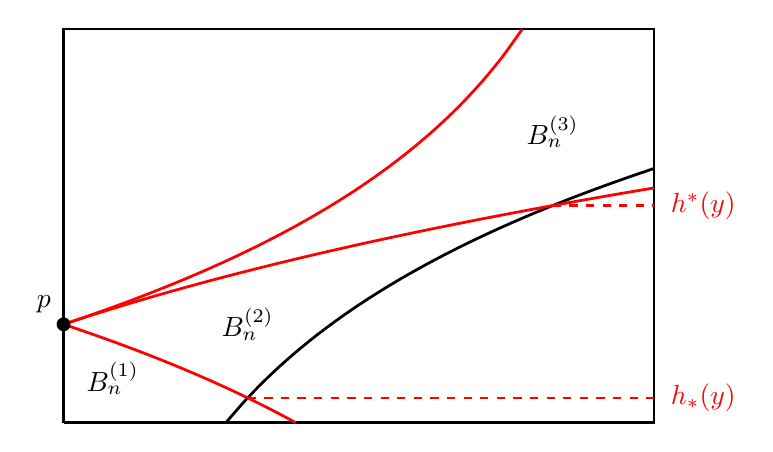
\begin{tikzpicture}[scale=1.25]

%%%%%%%%%%%%%%%%%%%%%%%%%%%%%%%%%%%%%%%%%%%%%%%%%%%%%%%%%%%%%%%%%%%%%%%%%%%%%%%%%%%%%%%%%%%%%%%%%%%
%																								  %
%	Shows the three different areas B_n^{(i)} for the computations in Lemma 					  %
%	\label{lem:clustering_error_T_term}			  												  %
%																								  %
%%%%%%%%%%%%%%%%%%%%%%%%%%%%%%%%%%%%%%%%%%%%%%%%%%%%%%%%%%%%%%%%%%%%%%%%%%%%%%%%%%%%%%%%%%%%%%%%%%%

	%Define the coordinates 
	%p = (\u,\v) and p^\prime = (\uu, \vv)
	%Box \Rcal_n has width 2\r and height \t
	\pgfmathsetmacro{\u}{0}
	\pgfmathsetmacro{\v}{1}
	\pgfmathsetmacro{\uu}{1.8}
	\pgfmathsetmacro{\vv}{1.7}
	\pgfmathsetmacro{\r}{6}
	\pgfmathsetmacro{\t}{4}
	
	%The box \Rcal_n only positive x
	\draw[line width=1pt] (0,0) -- (\r,0) -- (\r,\t) -- (0,\t) -- (0,0);	
	
	%Boundaries p = (\u,\v)
	
	%Right boundary
	\pgfmathsetmacro{\rightbounduv}{\u+exp((\v)/2)}
	\draw[domain=\rightbounduv:\r,smooth,variable=\x,black,line width=1pt] plot (\x, {2*ln(\x)-\v});
    %Left boundary
%    \pgfmathsetmacro{\leftbounduv}{\u-exp((\v)/2)}
%    \draw[domain=\leftbounduv:-\r,smooth,variable=\x,black,line width=1pt] plot (\x, {2*ln(-\x)-\v});
    
    %Three boundaries for the regions B_n
    \pgfmathsetmacro{\bone}{\r*(1-exp(-\v/2))}
    \pgfmathsetmacro{\btwo}{\r*(exp(-\v/2)-1)}
    %Star boundary
    \pgfmathsetmacro{\bthreeleft}{\r*(1-exp(\v/2))}
    \pgfmathsetmacro{\bthreeright}{\r*(1-exp((\v-\t)/2))}
    
    \draw[domain=0:\bone,smooth,variable=\x,red,line width=1pt] plot (\x, {\v-2*ln(\r/(\r-\x))});
    \draw[domain=0:\r,smooth,variable=\x,red,line width=1pt] plot (\x, {\v+2*ln(1+(\x/\r))});
    \draw[domain=0:\bthreeright,smooth,variable=\x,red, line width=1pt] plot (\x, {2*ln((\r/(\r-\x)))+\v});    
    
    %Define the top and bottom coordinates of y^prime boundaries
    \pgfmathsetmacro{\ybottom}{\v+2*ln(\r/(\r+exp(\v)))}
    \pgfmathsetmacro{\xbottom}{\r*exp(\v)/(\r + exp(\v))}
    \pgfmathsetmacro{\ytop}{\v+2*ln(\r/(\r-exp(\v)))}
    \pgfmathsetmacro{\xtop}{\r*exp(\v)/(\r - exp(\v))}
    
    \draw[dashed,line width=1pt,red] (\xbottom,\ybottom) -- (\r,\ybottom);
    \draw[dashed,line width=1pt,red] (\xtop,\ytop) -- (\r,\ytop);
    \draw node at (\r+0.5,\ybottom) {\color{red}$h_\ast(y)$};
    \draw node at (\r+0.5,\ytop) {\color{red}$h^\ast(y)$};
    
    \draw node at (0.5,\ybottom+0.2) {$B_n^{(1)}$};
    \draw node at (\xbottom,\ybottom+0.75) {$B_n^{(2)}$};
    \draw node at (\xtop,\ytop+0.75) {$B_n^{(3)}$};
    

    %Define h_1(p) = h_2(p)
    \pgfmathsetmacro{\hp}{2*ln(\r-\u)-\v}
  
    %Define h_1(p^\prime) and h_2(p^\prime)
    \pgfmathsetmacro{\hh}{2*ln(\uu+\r)-\vv}
    \pgfmathsetmacro{\hhh}{2*ln(\r-\uu)-\vv}

%    \draw node at (-\r-0.75,\hh+0.1) {\color{blue}$h_1(p^\prime)$};
%    \draw node at (\r+0.75,\hhh) {\color{blue}$h_2(p^\prime)$}; 
    
   	%Draw node p
    \draw node[fill, circle, inner sep=0pt, minimum size=5pt] (p1) at (\u,\v) {};
    \path (p1)+(-0.2,0.2) node {$p$};

\end{tikzpicture}
\caption{Three different areas $B_n^{(i)}$ used in the proof of Lemma \ref{lem:clustering_error_T_term}.}
\label{fig:comparing_triangles_B_areas}
\end{figure}

\begin{proof}[Proof of Lemma \ref{lem:clustering_error_T_term}]
Due to symmetry it is enough to show that
\begin{equation}\label{eq:clustering_error_T_main}
	\int_0^{R_n}\int_0^{I_n} \mu_{\alpha, \nu}\left(\mathcal{T}_{\Pcal \Delta \Pcal_n}(p,p_1)\right) f_{\mu, \nu}(x_1,y_1) 
	\dd x_1 \dd y_1 = \bigO{y n^{-(2\alpha - 1)} + n^{-(2\alpha-1)} e^{y}}
\end{equation}
The proof goes in two stages. First we compute $\mu_{\alpha, \nu}\left(\mathcal{T}_{\Pcal \Delta \Pcal_n}(p,p_1)\right)$ by splitting it over three disjoint regimes with respect to $p_1$, with $x_1 \ge 0$. Then we do the integration with respect to $p_1$.

\subsubsection*{Computing $\bm{\mu_{\alpha, \nu}\left(\mathcal{T}_{\Pcal \Delta \Pcal_n}(p,p_1)\right)}$}

Recall that $I_n = \frac{\pi}{2} e^{R_n/2}$ and define the sets
\begin{align*}
	A_n^{(1)} &= \left\{p_1 \in \Rcal_n \, : \, 0 \le y_1 \le y - 2\log(I_n/(I_n-x_1)) \right\},\\
	A_n^{(2)} &= \left\{p_1 \in \Rcal_n \, : \, y - 2\log(I_n/(I_n-x_1)) < y_1 
		\le y + 2 \log\left(1 + \frac{x_1}{I_n}\right)\right\},\\
	A_n^{(3)} &= \left\{p_1 \in \Rcal_n \, : \, y + 2 \log\left(1 + \frac{x_1}{I_n}\right) < y_1 
			\le y + 2 \log\left(\frac{I_n}{I_n-x_1}\right)\right\},
\end{align*}
and let $B_n^{(i)} = \BallPon{p} \cap A_n^{(i)}$, for $i = 1, 2, 3$, see Figure~\ref{fig:comparing_triangles_B_areas}. Here the heights of the two intersections are given by
\begin{align}
	h_\ast(y) &= y + 2 \log\left(\frac{I_n}{I_n + e^y}\right)\\
	h^\ast(y) &= y + 2 \log\left(\frac{I_n}{I_n - e^y}\right).
\end{align}

With these definitions we have that the union $B_n := \bigcup_{i = 1}^n B_n^{(i)}$ denotes the area under the red curve in Figure~\ref{fig:comparing_triangles_diff_analysis} and hence, for all $p_1 \in \Rcal_n\setminus B_n$ with $x_1 \ge 0$ we have that $\mathcal{T}_{\Pcal \Delta \Pcal_n}(p,p_1) = \emptyset$. So we only need to consider $p_1 \in B_n$. We shall establish the following result:
\begin{equation}\label{eq:mu_triangle_diff}
	\mu_{\alpha, \nu}\left(\mathcal{T}_{\Pcal \Delta \Pcal_n}(p,p_1)\right) = 
	\begin{cases}
		\bigO{I_n^{-2\alpha} e^{\alpha y_1}} &\mbox{if } p_1 \in B_n^{(1)}\\
		\bigO{I_n^{-2\alpha} e^{\alpha y}} &\mbox{if } p_1 \in B_n^{(2)} \cup B_n^{(3)}
	\end{cases}
\end{equation}

Depending on which regime $p_1$ belongs to, the set $\mathcal{T}_{\Pcal \Delta \Pcal_n}(p,p_1)$ has a different shape. We displayed these shapes in Figure~\ref{fig:shapes_triangle_mismatches} as a visual aid to follow the computations below. 

\begin{figure}[!tp]
\centering
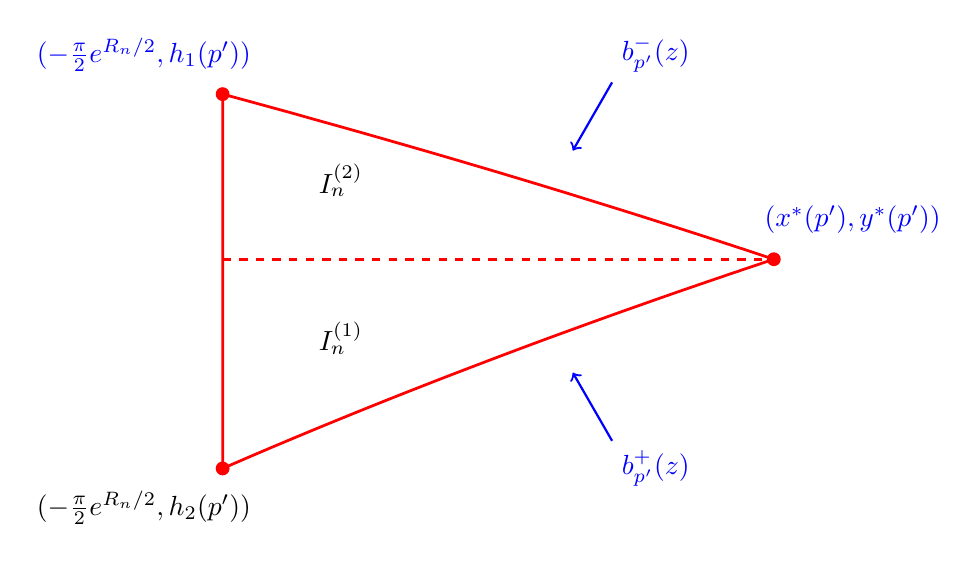
\begin{tikzpicture}[scale=5]

%%%%%%%%%%%%%%%%%%%%%%%%%%%%%%%%%%%%%%%%%%%%%%%%%%%%%%%%%%%%%%%%%%%%%%%%%%%%%%%%%%%%%%%%%%%%%%%%%%%
%																								  %
%	Shows the area T_{\Pcal \Delta \Pcal_n} when h_1(p^\prime) > h_2(p^\prime) > h(y)			  %
%																								  %
%%%%%%%%%%%%%%%%%%%%%%%%%%%%%%%%%%%%%%%%%%%%%%%%%%%%%%%%%%%%%%%%%%%%%%%%%%%%%%%%%%%%%%%%%%%%%%%%%%%

	%Define the coordinates 
	%p = (\u,\v) and p^\prime = (\uu, \vv)
	%Box \Rcal_n has width 2\r and height \t
	\pgfmathsetmacro{\u}{0}
	\pgfmathsetmacro{\v}{1}
	\pgfmathsetmacro{\uu}{1.4}
	\pgfmathsetmacro{\vv}{0.2}
	\pgfmathsetmacro{\r}{6}
	\pgfmathsetmacro{\t}{4}
    
    %Define x^\ast(p^\prime) and y^\ast(p^\prime)
    \pgfmathsetmacro{\uuast}{\uu-\r}
    \pgfmathsetmacro{\vvast}{2*ln(\r)-\vv}
    
    %Define intersection left black and shifted blue curve
    \pgfmathsetmacro{\vast}{2*ln((2*\r - \uu)/(exp(\v/2) + exp(\vv/2)))}
    \pgfmathsetmacro{\uast}{(\uu - 2*\r)/(1 + exp((\vv - \v)/2))}    
   
    %Define h_1(p) = h_2(p)
    \pgfmathsetmacro{\hp}{2*ln(\r-\u)-\v}
    
    %Define h_1(p^\prime) and h_2(p^\prime)
    \pgfmathsetmacro{\hh}{2*ln(\uu+\r)-\vv}
    \pgfmathsetmacro{\hhh}{2*ln(\r-\uu)-\vv}
    
    %Draw the boundary left black, left blue and shifted right blue line
	\draw[red,line width=1pt] 
		plot[domain=\uuast:-\r,smooth,variable=\x,red] (\x, {2*ln(\x+(2*\r-\uu))-\vv}) 
		-- 
		(-\r,\hh)
		-- 
		plot[domain=-\r:\uuast,smooth,variable=\x,red] (\x, {2*ln(\uu-\x)-\vv});
	
	\pgfmathsetmacro{\top}{2*ln(\uu-\uast)-\vv}
	
	\draw[red, dashed,line width=1pt] (-\r,\vvast) -- (\uuast,\vvast);

    \draw node at (-\r-0.2,\hh+0.1) {\color{blue}$(-\frac{\pi}{2} e^{R_n/2}, h_1(p^\prime))$};
    \draw node at (-\r-0.2,\hhh-0.1) {$(-\frac{\pi}{2} e^{R_n/2}, h_2(p^\prime))$};
    \draw node at (\uuast+0.2,\vvast+0.1) {\color{blue}$(x^\ast(p^\prime), y^\ast(p^\prime))$};
    
    \draw node at (-\r+0.3,\vvast+0.2) {$I_n^{(2)}$};
    \draw node at (-\r+0.3,\vvast-0.2) {$I_n^{(1)}$};
    
    \draw node (f2) at (\uuast-0.3,\hh+0.1) {\color{blue}$b_{p^\prime}^-(z)$};
    \draw node (f3) at (\uuast-0.3,\hhh) {\color{blue}$b_{p^\prime}^+(z)$};
    \path (f2)+(230:0.35) node (f2_arrow) {};
    \path (f3)+(130:0.35) node (f3_arrow) {};
    \draw[->,thick,blue] (f2.south west) -- (f2_arrow);
    \draw[->,thick,blue] (f3.north west) -- (f3_arrow);

	\draw node[red, fill, circle, inner sep=0pt, minimum size=5pt] at (-\r,\hhh) {};
	\draw node[red, fill, circle, inner sep=0pt, minimum size=5pt] at (-\r,\hh) {};
	\draw node[red, fill, circle, inner sep=0pt, minimum size=5pt] at (\uuast,\vvast) {};

\end{tikzpicture}\\
\vspace{20pt}
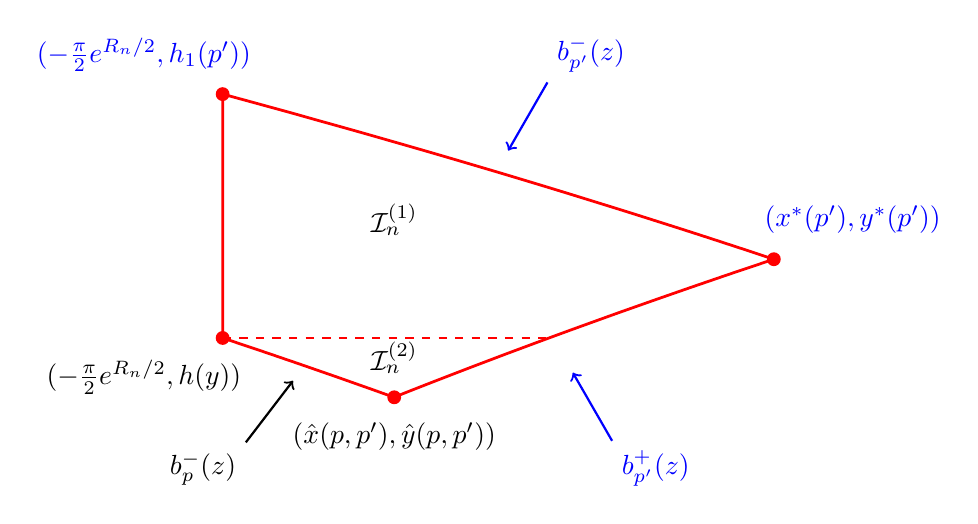
\begin{tikzpicture}[scale=5]
	%Define the coordinates 
	%p = (\u,\v) and p^\prime = (\uu, \vv)
	%Box \Rcal_n has width 2\r and height \t
	\pgfmathsetmacro{\u}{0}
	\pgfmathsetmacro{\v}{1}
	\pgfmathsetmacro{\uu}{1.4}
	\pgfmathsetmacro{\vv}{0.8}
	\pgfmathsetmacro{\r}{6}
	\pgfmathsetmacro{\t}{4}
    
    %Define x^\ast(p^\prime) and y^\ast(p^\prime)
    \pgfmathsetmacro{\uuast}{\uu-\r}
    \pgfmathsetmacro{\vvast}{2*ln(\r)-\vv}
    
    %Define intersection left black and shifted blue curve
    \pgfmathsetmacro{\vast}{2*ln((2*\r - \uu)/(exp(\v/2) + exp(\vv/2)))}
    \pgfmathsetmacro{\uast}{(\uu - 2*\r)/(1 + exp((\vv - \v)/2))}    
   
    %Define h_1(p) = h_2(p)
    \pgfmathsetmacro{\hp}{2*ln(\r-\u)-\v}
    
    %Define h_1(p^\prime) and h_2(p^\prime)
    \pgfmathsetmacro{\hh}{2*ln(\uu+\r)-\vv}
    \pgfmathsetmacro{\hhh}{2*ln(\r-\uu)-\vv}
    
    %Draw the boundary left black, left blue and shifted right blue line
	\draw[red,line width=1pt] 
		plot[domain=\uuast:\uast,smooth,variable=\x,red] (\x, {2*ln(\x+(2*\r-\uu))-\vv}) 
		-- 
		plot[domain=\uast:-\r,smooth,variable=\x,red] (\x, {2*ln(-\x)-\v})
		-- 
		(-\r,\hh)
		-- 
		plot[domain=-\r:\uuast,smooth,variable=\x,red] (\x, {2*ln(\uu-\x)-\vv});
	
	\pgfmathsetmacro{\rb}{\uu + exp((\vv+\hp)/2) -2*\r}
	

	%\draw[red,dashed,line width=1pt] (\uast,\vast) -- (\uast,\hp);
	\draw[red,dashed,line width=1pt] (-\r,\hp) -- (\rb,\hp);

    \draw node at (-\r-0.2,\hh+0.1) {\color{blue}$(-\frac{\pi}{2} e^{R_n/2}, h_1(p^\prime))$};
    \draw node at (-\r-0.2,\hp-0.1) {$(-\frac{\pi}{2} e^{R_n/2}, h(y))$};
    \draw node at (\uuast+0.2,\vvast+0.1) {\color{blue}$(x^\ast(p^\prime), y^\ast(p^\prime))$};
    \draw node at (\uast,\vast-0.1) {$(\hat{x}(p,p^\prime), \hat{y}(p, p^\prime))$};
    
    \draw node at (\uast,\vvast+0.1) {$\mathcal{I}_n^{(1)}$};
    \draw node at (\uast,\hp-0.05) {$\mathcal{I}_n^{(2)}$};
    %\draw node at (\uast+0.1,\hp-0.05) {$\mathcal{I}_n^{(3)}$};
    
    \draw node (f1) at (-\r-0.05,\hhh) {$b_p^-(z)$};
    \draw node (f2) at (\uast+0.5,\hh+0.1) {\color{blue}$b_{p^\prime}^-(z)$};
    \draw node (f3) at (\uuast-0.3,\hhh) {\color{blue}$b_{p^\prime}^+(z)$};
    \path (f1)+(45:0.35) node (f1_arrow) {};
    \path (f2)+(230:0.35) node (f2_arrow) {};
    \path (f3)+(130:0.35) node (f3_arrow) {};
    \draw[->,thick] (f1.north east) -- (f1_arrow);
    \draw[->,thick,blue] (f2.south west) -- (f2_arrow);
    \draw[->,thick,blue] (f3.north west) -- (f3_arrow);

	\draw node[red, fill, circle, inner sep=0pt, minimum size=5pt] at (-\r,\hp) {};
	\draw node[red, fill, circle, inner sep=0pt, minimum size=5pt] at (-\r,\hh) {};
	\draw node[red, fill, circle, inner sep=0pt, minimum size=5pt] at (\uuast,\vvast) {};
	\draw node[red, fill, circle, inner sep=0pt, minimum size=5pt] at (\uast,\vast) {};

\end{tikzpicture}\\
\vspace{20pt}
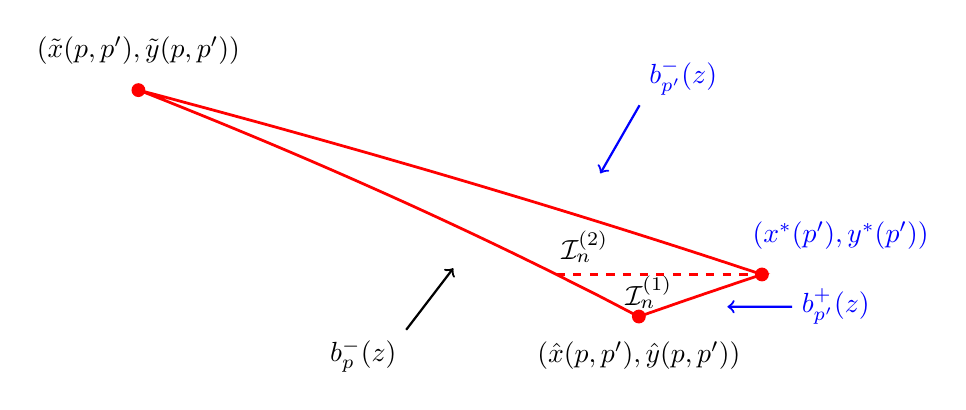
\begin{tikzpicture}[scale=5]

%%%%%%%%%%%%%%%%%%%%%%%%%%%%%%%%%%%%%%%%%%%%%%%%%%%%%%%%%%%%%%%%%%%%%%%%%%%%%%%%%%%%%%%%%%%%%%%%%%%
%																								  %
%	Shows the area T_{\Pcal \Delta \Pcal_n} when h(y) > h_1(p^\prime)							  %
%																								  %
%%%%%%%%%%%%%%%%%%%%%%%%%%%%%%%%%%%%%%%%%%%%%%%%%%%%%%%%%%%%%%%%%%%%%%%%%%%%%%%%%%%%%%%%%%%%%%%%%%%

	%Define the coordinates 
	%p = (\u,\v) and p^\prime = (\uu, \vv)
	%Box \Rcal_n has width 2\r and height \t
	\pgfmathsetmacro{\u}{0}
	\pgfmathsetmacro{\v}{1}
	\pgfmathsetmacro{\uu}{2.5}
	\pgfmathsetmacro{\vv}{1.8}
	\pgfmathsetmacro{\r}{6}
	\pgfmathsetmacro{\t}{4}
    
    %Define x^\ast(p^\prime) and y^\ast(p^\prime)
    \pgfmathsetmacro{\uuast}{\uu-\r}
    \pgfmathsetmacro{\vvast}{2*ln(\r)-\vv}
    
    %Define intersection left black and shifted blue curve
    \pgfmathsetmacro{\vast}{2*ln((2*\r - \uu)/(exp(\v/2) + exp(\vv/2)))}
    \pgfmathsetmacro{\uast}{(\uu - 2*\r)/(1 + exp((\vv - \v)/2))}    
    
    %Define intersection left black and left blue curve
    \pgfmathsetmacro{\utilde}{\uu/(1-exp((\vv-\v)/2))} 
    \pgfmathsetmacro{\vtilde}{2*ln(\uu-\utilde)-\vv}
   
    %Define h_1(p) = h_2(p)
    \pgfmathsetmacro{\hp}{2*ln(\r-\u)-\v}
    
    %Define h_1(p^\prime) and h_2(p^\prime)
    \pgfmathsetmacro{\hh}{2*ln(\uu+\r)-\vv}
    \pgfmathsetmacro{\hhh}{2*ln(\r-\uu)-\vv}
    
    %Draw the boundary left black, left blue and shifted right blue line
	\draw[red,line width=1pt] 
		plot[domain=\utilde:\uuast,smooth,variable=\x,red] (\x, {2*ln(\uu-\x)-\vv})
		--
		plot[domain=\uuast:\uast,smooth,variable=\x,red] (\x, {2*ln(\x+(2*\r-\uu))-\vv})
		--
		plot[domain=\uast:\utilde,smooth,variable=\x,red] (\x, {2*ln(-\x)-\v}); 
	
	%Calculate intersection point
	\pgfmathsetmacro{\i}{-exp((\v+\vvast)/2)}
	\draw[red, dashed,line width=1pt] (\i,\vvast) -- (\uuast,\vvast);

    \draw node at (\utilde,\vtilde+0.1) {\color{black}$(\tilde{x}(p,p^\prime), \tilde{y}(p,p^\prime))$};
    \draw node at (\uast,\vast-0.1) {$(\hat{x}(p,p^\prime), \hat{y}(p,p^\prime))$};
    \draw node at (\uuast+0.2,\vvast+0.1) {\color{blue}$(x^\ast(p^\prime), y^\ast(p^\prime))$};
   
    \draw node at (\uuast-0.45,\vvast+0.07) {$\mathcal{I}_n^{(2)}$};
    \draw node at (\uast+0.025,\vvast-0.045) {$\mathcal{I}_n^{(1)}$};
   
    \draw node (f1) at (\uast-0.7,\vast-0.1) {\color{black}$b_{p}^-(z)$};
    \draw node (f2) at (\uuast-0.2,\vvast+0.5) {\color{blue}$b_{p^\prime}^-(z)$};
    \draw node (f3) at (\uast+0.5,\vast+0.025) {\color{blue}$b_{p^\prime}^+(z)$};
    \path (f1)+(45:0.35) node (f1_arrow) {};
    \path (f2)+(230:0.35) node (f2_arrow) {};
    \path (f3)+(180:0.3) node (f3_arrow) {};
	\draw[->,thick] (f1.north east) -- (f1_arrow);
    \draw[->,thick,blue] (f2.south west) -- (f2_arrow);
    \draw[->,thick,blue] (f3.west) -- (f3_arrow);
%
	\draw node[red, fill, circle, inner sep=0pt, minimum size=5pt] at (\utilde,\vtilde) {};
	\draw node[red, fill, circle, inner sep=0pt, minimum size=5pt] at (\uast,\vast) {};
	\draw node[red, fill, circle, inner sep=0pt, minimum size=5pt] at (\uuast,\vvast) {};

\end{tikzpicture}
\caption{The different shapes of $\mathcal{T}_{\Pcal \Delta \Pcal_n}(p,p_1)$ depending on the regime to which $p_1$ belongs. The top figure is for $p_1 \in B_n^{(1)}$, the middle for $p_1 \in B_n^{(2)}$ and the bottom one for $p_1 \in B_n^{(3)}$.}
\label{fig:shapes_triangle_mismatches}
\end{figure}

\paragraph{Regime 1: $0 \le y_1 \le y - 2\log(I_n/(I_n-x_1))$}

In this case the integral over $p_2$ splits into two parts
\begin{align*}
	\mathcal{I}_n^{(1)}(p_1) &:= \int_{h_2(p_1)}^{y^\ast(p_1)} \int_{-I_n}^{x_1 + e^{(y_1+y_2)/2}-2I_n} e^{-\alpha y_2}
		\dd x_2 \dd y_2\\
	\mathcal{I}_n^{(2)}(p_1) &:= \int_{y^\ast(p_1)}^{h_1(p_1)} \int_{x^\ast(p_1)}^{x_1 - e^{(y_1+y_2)/2}} e^{-\alpha y_2}
		\dd x_2 \dd y_2.
\end{align*}

We first compute $\mathcal{I}_n^{(1)}$.
\begin{align*}
	\mathcal{I}_n^{(1)}(p_1) &= \int_{h_2(p_1)}^{y^\ast(p_1)} \left(x_1 + e^{(y_1+y_2)/2} - I_n\right) e^{-\alpha y_2} 
		\dd x_2 \dd y_2\\
	&\le e^{y_1/2} \int_{h_2(p_1)}^{y^\ast(p_1)} e^{-(\alpha-\frac{1}{2}) y_2} \dd y_2\\
	&= \frac{2 e^{y_1/2}}{2\alpha - 1} \left(e^{-(\alpha-\frac{1}{2})h_2(p_1)} - e^{-(\alpha-\frac{1}{2})y^\ast(p_1)}
		\right) \\
	&= \frac{2 e^{\alpha y_1}}{2\alpha - 1} I_n^{-(2\alpha -1)}\left(\left(1 - \frac{x_1}{I_n}\right)^{-(2\alpha - 1)}-1\right)\\
	&= \bigO{I_n^{-2\alpha} x_1 e^{\alpha y_1}},
\end{align*}
where we used that $x^\prime \le e^{(y+y_1)/2} = \smallO{I_n}$ for all $y_1\le y$ and $y \in \Kcal_{C}(k_n)$ so that
\[
	\left(\left(1 - \frac{x_1}{I_n}\right)^{-(2\alpha - 1)}-1\right) = \bigO{\frac{x^\prime}{I_n}} \quad 
	\text{as } n \to \infty.
\]

For $\mathcal{I}_n^{(2)}(p_1)$ we have
\begin{align*}
	\mathcal{I}_n^{(2)}(p_1) &= \int_{y^\ast(p_1)}^{h_1(p_1)} \left(I_n + x_1 - e^{(y_1+y_2)}\right) e^{-\alpha y_2}
		\dd x_2 \dd y_2\\
	&\le 2 I_n \int_{y^\ast(p_1)}^{h_1(p_1)} e^{-\alpha y_2} \dd x_2 \dd y_2\\
	&= \frac{2}{\alpha} I_n \left(I_n^{-2\alpha}e^{\alpha y_1} - \left(I_n + x_1\right)^{-2\alpha} e^{-\alpha y_1}\right)\\
	&= \bigO{I_n^{-2\alpha} x_1 e^{\alpha y_1}} = \bigO{I_n^{-(2\alpha - 1)} e^{\alpha y_1}}.
\end{align*}

We conclude that for $p_1 \in B_n^{(1)}$:
\[
	\mu_{\alpha, \nu}\left(\mathcal{T}_{\Pcal \Delta \Pcal_n}(p,p_1)\right) = \bigO{I_n^{-2\alpha} x_1 e^{\alpha y_1}},
\]
which establishes the first part of \eqref{eq:mu_triangle_diff}.

\paragraph{Regime 2: $y - 2\log(I_n/(I_n-x_1)) < y_1 \le y + 2 \log\left(1 + \frac{x_1}{I_n}\right)$}

Here we split the integration into two parts (see Figure~\ref{fig:shapes_triangle_mismatches}). Recall that $x^\ast(p,p_1) = x_1 - I_n$. Then, for the first part we have
\begin{align*}
	\mathcal{I}_n^{(1)}(p,p_1) &\le \int_{h(y)}^{h_1(p_1)} \int_{-I_n}^{x^\ast(p,p_1)} f_{\alpha,\nu}(x_2, y_2) 
		\dd x_2 \dd y_2\\
	&= \bigO{x_1 \left(e^{-\alpha h(y)} - e^{-\alpha h_1(p_1)}\right)}\\
	&= \bigO{x_1 I_n^{-2\alpha}\left(e^{\alpha y} - e^{\alpha y_1}\left(1 + \frac{x_1}{I_n}\right)^{-2\alpha}\right)}\\
	&= \bigO{I_n^{-2\alpha} x_1 e^{\alpha y_1}\left(\left(1 - \frac{x_1}{I_n}\right)^{-2\alpha} 
		- \left(1 + \frac{x_1}{I_n}\right)^{-2\alpha}\right)}\\
	&= \bigO{I_n^{-2\alpha} x_1 e^{\alpha y_1}} = \bigO{I_n^{-(2\alpha - 1)} e^{\alpha y}}, 
\end{align*}
were we used that $y \le y_1 + 2\log(I_n/(I_n-x_1))$ for $p_1 \in B_n^{(2)}$ for the third line and 
\[
	\left(1 - \frac{x_1}{I_n}\right)^{-2\alpha} - \left(1 + \frac{x_1}{I_n}\right)^{-2\alpha}
	= \bigO{\frac{x_1}{I_n}} = \bigO{1},
\]
for the last line.

For the second part we first compute that 
\begin{align*}
	x_1 + e^{(y_1+y_2)/2} - 2 I_n + e^{(y + y_2)/2} &\le \left(e^{y/2} + e^{y_1/2}\right)e^{y_2/2}\\
	&\le e^{y/2}\left(1 + \frac{I_n}{I_n - e^y}\right)e^{y_2/2} = \bigO{e^{(y+y_2)/2}},
\end{align*}
since $y \in \Kcal_{C}(k_n)$ and $k_n = \smallO{\sqrt{n}}$, so that $e^y = \smallO{n} = \smallO{I_n}$. 
Then we have
\begin{align*}
	\mathcal{I}_n^{(2)} &= \int_{\hat{y}(p,p_1)}^{h(y)} \int_{-e^{(y + y_2)/2}}^{x_1 + e^{(y+y_1)/2} - 2 I_n} 
		f_{\alpha,\nu}(x_2, y_2) \dd x_2 \dd y_2\\
	&= \bigO{e^{y/2} \int_{\hat{y}(p,p_1)}^{h(y)} e^{-(\alpha -\frac{1}{2}) y_2} \dd y_2}\\
	&= \bigO{e^{y/2} \left(e^{-(\alpha -\frac{1}{2}) \hat{y}(p,p_1)} - e^{-(\alpha -\frac{1}{2}) h(y)}\right)}\\
	&= \bigO{e^{y/2} \left(\left(\frac{2I_n - x_1}{e^{y/2} + e^{y_1/2}}\right)^{-(2\alpha-1)} 
		- I_n^{-(2\alpha-1)} e^{(\alpha -\frac{1}{2}) y}\right)}\\
	&= \bigO{I_n^{-(2\alpha-1)} e^{\alpha y}},
\end{align*}
where for the last line we first used that $(2I_n - x_1)^{-(2\alpha-1)} \le I_n^{-(2\alpha-1)}$ and then
\[
	\left(\left(e^{y/2} + e^{y_1/2}\right)^{2\alpha-1}- e^{(\alpha -\frac{1}{2}) y}\right)
	\le e^{(\alpha -\frac{1}{2}) y}\left(\left(1 + \sqrt{1+\frac{x_1}{I_n}} \, \right)^{2\alpha - 1} - 1\right)
	= \bigO{e^{(\alpha -\frac{1}{2}) y}}.
\]

It then follows that for $p_1 \in B_n^{(2)}$
\[
	\mu_{\alpha, \nu}\left(\mathcal{T}_{\Pcal \Delta \Pcal_n}(p,p_1)\right) = \bigO{I_n^{-(2\alpha-1)} e^{\alpha y}}.
\]

\paragraph{Regime III $\bm{p_1 \in B_n^{(3)}}$:}

\begin{align*}
	\mathcal{I}_n^{(1)} &= \int_{y^\ast}^{\tilde{y}} \int_{-e^{(y+y_2)/2}}^{x_1-e^{(y_1+y_2)/2}} f_{\alpha, \nu}(x_2,y_2)
		\dd x_2 \dd y_2\\
	&= \bigO{\int_{y^\ast}^{\tilde{y}} x_1 e^{-\alpha y_2} - \left(e^{y_1/2} - e^{y/2}\right)e^{-(\alpha - \frac{1}{2})y_2}
		\dd y_2}\\
	&= \bigO{x_1 \int_{y^\ast}^{\tilde{y}}  e^{-\alpha y_2} \dd y_2}.
\end{align*}

Now 
\begin{align*}
	\int_{y^\ast}^{\tilde{y}}  e^{-\alpha y_2} \dd y_2 
	&= \frac{1}{\alpha}\left(e^{-\alpha y^\ast} - e^{-\alpha \tilde{y}}\right) 
		= \frac{1}{\alpha}\left(I_n^{-2\alpha} e^{\alpha y_1} 
		- \left(\frac{x_1}{e^{y_1/2} - e^{y/2}}\right)^{-2\alpha}\right) \\
	&= \frac{I_n^{-2\alpha} e^{\alpha y_1}}{\alpha}\left(1 - \left(1 - e^{(y - y_1)/2}\right)^{2\alpha}
		\left(\frac{x_1}{I_n}\right)^{-2\alpha}\right) = \bigO{I_n^{-2\alpha} e^{\alpha y_1}},
\end{align*}
and hence we have
\[
	\mathcal{I}_n^{(1)} = \bigO{I_n^{-2\alpha} x_1 e^{\alpha y_1}}.
\]

For the second integral we have
\begin{align*}
	\mathcal{I}_n^{(2)} &= \int_{\hat{y}}^{y^\ast} \int_{-e^{(y+y_2)/2}}^{e^{(y_1 + y_2)/2} + x_1 - 2I_n} 
		f_{\alpha, \nu}(x_2,y_2)\dd x_2 \dd y_2\\
	&= \bigO{\int_{\hat{y}}^{y^\ast} \left(e^{y/2} + e^{y_1/2}\right)e^{-(\alpha - \frac{1}{2})y_2} \dd y_2}\\
	&= \bigO{ e^{y_1/2} \int_{\hat{y}}^{y^\ast}e^{-(\alpha - \frac{1}{2})y_2} \dd y_2}.
\end{align*}

For the integral we have
\begin{align*}
	\int_{\hat{y}}^{y^\ast}e^{-(\alpha - \frac{1}{2})y_2} \dd y_2
	&= \frac{2}{2\alpha - 1} \left(e^{-(\alpha - \frac{1}{2})\hat{y}} - e^{-(\alpha - \frac{1}{2})y^\ast}\right)\\
	&= \frac{2}{2\alpha - 1}\left(\left(\frac{2I_n - x_1}{e^{y/2} + e^{y_1/2}}\right)^{-(2\alpha - 1)} 
		- I_n^{-(2\alpha - 1)} e^{-(\alpha - \frac{1}{2})y_1}\right)\\
	&= \bigO{I_n^{-2\alpha} x_1 e^{-(\alpha - \frac{1}{2})y_1}}
\end{align*}
so that
\[
	\mathcal{I}_n^{(2)} = \bigO{I_n^{-(2\alpha - 1)} e^{(1-\alpha)y_1}} = \bigO{I_n^{-2\alpha} x_1 e^{\alpha y}}
\]
and hence for $p_1 \in B_n^{(3)}$
\[
	\mu_{\alpha, \nu}\left(\mathcal{T}_{\Pcal \Delta \Pcal_n}(p,p_1)\right) = \bigO{I_n^{-2\alpha} x_1 e^{\alpha y}}
	= \bigO{I_n^{-(2\alpha - 1)} e^{\alpha y}}.
\]

\subsubsection*{Integration over $p_1$}



We now proceed with the second part of the computation leading to \eqref{eq:clustering_error_T_main}. Here we will integrate $\mu_{\alpha, \nu}(\mathcal{T}_{\Pcal \Delta \Pcal_n})(p,p_1)$ over the region $B_n := B_n^{(1)} \cup B_n^{(2)} \cup B_n^{(3)}$, see Figure~\ref{fig:comparing_triangles_B_areas}. Let us first identify the boundaries of these areas. 

The area $B_n^{(1)}$ is bounded from above by the line given by the equation
\[
	y_1 = y - 2\log\left(\frac{I_n}{I_n - x_1}\right).
\]
Solving this for $x_1$ yields $x_1 = I_n\left(1 - e^{(y_1-y)/2}\right)$ and hence the area $B_n^{(1)}$ is given by
\[
	B_n^{(1)} = \left\{(x_1, y_1) \, : \, 0 \le y_1 \le y, \quad 0 \le x_1 \le I_n\left(1 - e^{(y_1-y)/2}\right) \wedge e^{(y + y_1)/2} \right\}.
\]

In a similar way we have that $B_n^{(2)}$ is bounded from above by line
\[
	y_1 = y + 2\log\left(\frac{I_n}{I_n + x_1}\right),
\]
which yields $x_1 = I_n\left(e^{(y_1 - y)/2} - 1\right)$. The lower red boundary is the upper boundary of $B_n^{(2)}$ and hence we have
\[
	B_n^{(2)} = \left\{(x_1, y_1) \, : \, h_\ast(y) \le y_1 \le h^\ast(y), \,\, I_n\left(1 - e^{(y_1-y)/2}\right) \vee 
	I_n\left(e^{(y_1 - y)/2} - 1\right) \le x_1 \le e^{(y + y_1)/2} \right\}.
\]

We continue is the same way to obtain for $B_n^{(3)}$
\[
	B_n^{(3)} = \left\{(x_1, y_1) \, : \, y \le y_1 \le R_n, \,\,
	I_n\left(1 - e^{(y - y_1)/2}\right) \le x_1 \le I_n\left(e^{(y_1 - y)/2} - 1\right) \wedge e^{(y + y_1)/2} \wedge I_n \right\}.
\]

We these characterizations of the areas we now integrate $\mu_{\alpha, \nu}(\mathcal{T}_{\Pcal \Delta \Pcal_n})(p,p_1)$ over $B_n$, splitting the computations over the three different areas.

\paragraph{$\bm{p_1 \in B_n^{(1)}}:$}

We use that $I_n\left(1 - e^{(y_1-y)/2}\right) \wedge e^{(y + y_1)/2} \le I_n\left(1 - e^{(y_1-y)/2}\right)$ so that
\begin{align*}
	&\hspace{-30pt}\int_{B_n^{(1)}} \mu_{\alpha, \nu}\left(\mathcal{T}_{\Pcal \Delta \Pcal_n}(p,p_1)\right) 
		f_{\alpha,\nu}(x_1,y_1)	\dd x_1 \dd y_1 \\
	&\le  \int_0^y \int_0^{I_n(1-e^{(y_1-y)/2})} \mu_{\alpha, \nu}\left(\mathcal{T}_{\Pcal \Delta \Pcal_n}(p,p_1)\right) 
		f_{\alpha,\nu}(x_1,y_1) \dd x_1 \dd y_1\\
	&= \bigO{ I_n^{-2\alpha} \int_0^y \int_0^{e^{(y+y_1)/2}}  x_1 \dd x_1 \dd y_1 }\\
	&= \bigO{I_n^{-(2\alpha-1)} \int_0^y \left(1 - e^{(y_1-y)/2}\right)^2 \dd y_1} \\
	&= \bigO{I_n^{-(2\alpha - 1)} y} = \bigO{y n^{-(2\alpha - 1)}}.
\end{align*} 

\paragraph{$\bm{p_1 \in B_n^{(2)}}:$}

We will show that
\begin{equation}\label{eq:mu_triangle_diff_2}
	\mu_{\alpha, \nu}(B_n^{(2)}) = \bigO{I_n^{-1} e^{(2-\alpha)y}},
\end{equation}
which together with \eqref{eq:mu_triangle_diff} yields
\begin{align*}
	\int_{B_n^{(2)}} \mu_{\alpha, \nu}\left(\mathcal{T}_{\Pcal \Delta \Pcal_n}(p,p_1)\right) 
		f_{\alpha,\nu}(x_1,y_1)	\dd x_1 \dd y_1
	&= \bigO{\mu_{\alpha, \nu}(B_n^{(2)}) I_n^{-(2\alpha - 1)} e^{\alpha y}}\\
	&= \bigO{I_n^{-2\alpha} e^{2y}}.
\end{align*}

The integration is split into two parts determined by $I_n\left(1 - e^{(y_1-y)/2}\right) \vee 
	I_n\left(e^{(y_1 - y)/2} - 1\right)$:
\begin{align*}
	\mu_{\alpha, \nu}(B_n^{(3)}) &= \int_{h_\ast(y)}^{y} \int_{I_n(1-e^{(y_1-y)/2})}^{e^{(y + y_1)/2}} 
		f_{\alpha,\nu}(x_1,y_1) \dd x_1 \dd y_1\\
	&\hspace{10pt} + \int_y^{h^\ast(y)} \int_{I_n(e^{(y_1-y)/2}-1)}^{e^{(y + y_1)/2}} 
		f_{\alpha,\nu}(x_1,y_1) \dd x_1 \dd y_1.
\end{align*}

For the first integral we use that $e^{(y + y_1)/2} - I_n(1-e^{(y_1-y)/2}) \le e^{y_1/2}\left(e^{y/2} + e^{-y/2}\right)$ to obtain
\begin{align*}
	&\hspace{-30pt}\int_{h_\ast(y)}^{y} \int_{I_n(1-e^{(y_1-y)/2})}^{e^{(y + y_1)/2}} f_{\alpha,\nu}(x_1,y_1) 
		\dd x_1 \dd y_1\\
	&= \bigO{e^{y/2} \int_{h_\ast(y)}^{y} e^{-(\alpha - \frac{1}{2})y_1} \dd y_1}\\
	&= \bigO{e^{y/2}\left(e^{-(\alpha - \frac{1}{2})y} - e^{-(\alpha - \frac{1}{2})y} 
		\left(\frac{I_n}{I_n + e^y}\right)^{-(2\alpha - 1)}\right)}\\
	&= \bigO{I_n^{-1} e^{(2-\alpha)y}}.
\end{align*}
For the second integral note that $e^{(y + y_1)/2} - I_n(e^{(y_1-y)/2}-1) \le e^{(y + y_1)/2}$ and hence
\begin{align*}
	&\hspace{-30pt}\int_y^{h^\ast(y)} \int_{I_n(e^{(y_1-y)/2}-1)}^{e^{(y + y_1)/2}} f_{\alpha,\nu}(x_1,y_1) 
		\dd x_1 \dd y_1\\
	&= \bigO{e^{y/2} \int_y^{h^\ast(y)} e^{-(\alpha - \frac{1}{2})y_1} \dd y_1}\\
	&= \bigO{e^{y/2} \left(e^{-(\alpha - \frac{1}{2})y} - e^{-(\alpha - \frac{1}{2})y}
		\left(\frac{I_n}{I_n - e^y}\right)^{-(2\alpha - 1)}\right)}\\
	&= \bigO{I_n^{-1} e^{(2-\alpha)y}},
\end{align*}
so that \eqref{eq:mu_triangle_diff_2} follows.

\paragraph{$\bm{p_1 \in B_n^{(3)}}:$}

For this area we show that 
\begin{equation}\label{eq:mu_triangle_diff_3}
	\mu_{\alpha, \nu}(B_n^{(3)}) = \bigO{e^{(1-\alpha)y}}
\end{equation} 
so that
\begin{align*}
	\int_{B_n^{(3)}} \mu_{\alpha, \nu}\left(\mathcal{T}_{\Pcal \Delta \Pcal_n}(p,p_1)\right) 
		f_{\alpha,\nu}(x_1,y_1)	\dd x_1 \dd y_1
	&= \bigO{\mu_{\alpha, \nu}(B_n^{(2)}) I_n^{-(2\alpha - 1)} e^{\alpha y}}\\
	&= \bigO{I_n^{-(2\alpha-1)} e^{y}}.
\end{align*}

Here the integral is split into three parts:
\begin{align*}
	\mu_{\alpha, \nu}(B_n^{(3)}) &= \int_y^{h^\ast(y)} \int_{I_n(1-e^{(y-y_1)/2})}^{I_n(e^{(y_1-y)/2}-1)}
		f_{\alpha,\nu}(x_1,y_1) \dd x_1 \dd y_1\\
	&\hspace{10pt}+ \int_{h^\ast(y)}^{h(y)} \int_{I_n(1-e^{(y-y_1)/2})}^{e^{(y+y_1)/2}}
		f_{\alpha,\nu}(x_1,y_1) \dd x_1 \dd y_1\\
	&\hspace{10pt}+ \int_{h(y)}^{R_n} \int_{I_n(1-e^{(y-y_1)/2})}^{I_n}
		f_{\alpha,\nu}(x_1,y_1) \dd x_1 \dd y_1.
\end{align*}

Let us first focus on the first integral. Since	$I_n(e^{(y_1-y)/2}-1) - I_n(1-e^{(y-y_1)/2}) \le I_n e^{(y_1-y)/2}$ we get,
using similar arguments as above
\begin{align*}
	\int_y^{h^\ast(y)} \int_{I_n(1-e^{(y-y_1)/2})}^{I_n(e^{(y_1-y)/2}-1)} f_{\alpha,\nu}(x_1,y_1) \dd x_1 \dd y_1
	&= \bigO{I_n e^{-y/2} \int_y^{h^\ast(y)} e^{-(\alpha - \frac{1}{2})y_1} \dd y_1}\\
	&= \bigO{I_n e^{-\alpha y} \left(1 - \left(\frac{I_n}{I_n - e^y}\right)^{-(2\alpha - 1)}\right)}\\
	&= \bigO{e^{(1-\alpha)y}}.
\end{align*}

Proceeding to the second integral, we first note that $e^{(y+y_1)/2} - I_n(1-e^{(y-y_1)/2}) = \bigO{I_n e^{(y_1-y)/2}}$ so that similar calculations as before yield
\begin{align*}
	\int_{h^\ast(y)}^{h(y)} \int_{I_n(1-e^{(y-y_1)/2})}^{e^{(y+y_1)/2}}	f_{\alpha,\nu}(x_1,y_1) \dd x_1 \dd y_1
	&= \bigO{I_n e^{-y/2} \int_{h^\ast(y)}^{h(y)} e^{-(\alpha - \frac{1}{2})y_1} \dd y_1}
		= \bigO{e^{(1-\alpha)y}}.
\end{align*}



\end{proof}

\section{Concentration for $c_{\mathcal{P}, n}(k)$ (Proving Proposition \ref{prop:concentration_local_clustering_P_n})}
\label{sec:concentration_c_P_n}

\subsection{The main contribution of triangles}

Recall the adjusted triangle count function \eqref{eq:def_tilde_triangle_indicator}
\[
	\widetilde{T}_{\Pcal,n}(p_0,p_1,p_2) = \ind{p_1 \in B_{\Pcal,n}(p)}\ind{p_2 \in B_{\Pcal,n}(p)}\ind{p_2 \in B_{\Pcal}(p_1) \cap \Rcal_n}.
\]
and the concentration set
\[
	\Kcal_C(k) = \left\{p \in \R : \frac{k - C \sqrt{k \log(k)}}{\xi_{\alpha,\nu}} \le e^{\frac{y}{2}}
		\le \frac{k + C \sqrt{k \log(k)}}{\xi_{\alpha,\nu}} \right\},
\]
We will define the corresponding triangle degree function
\begin{equation}\label{eq:def_degree_triangle_count_in_K}
	\widetilde{T}_{\Pcal,n}(k,C) = \sum_{p \in \Pcal_n \cap K_C(k)} \ind{D_{\Pcal,n}(p) = k} \widetilde{T}_{\Pcal,n}(p),
\end{equation}
where
\[
	\widetilde{T}_{\Pcal,n}(p) := \sum_{(p_1, p_2) \in 2^{\Pcal_n}} \widetilde{T}_{\Pcal,n}(p,p_1,p_2).
\]

By Lemma \ref{lem:clustering_error_T_term} and a concentration argument it follows that for $k_n \to \infty$
\[
	\Exp{\widetilde{T}_{\Pcal,n}(k_n,C)} = (1+\smallO{1})\Exp{T_{\Pcal}(k_n)},
\]
for a appropriately selected $C > 0$. We conclude that the main contribution of triangles of degree $k_n$ is given by $\widetilde{T}_{\Pcal,n}(k_n,C)$. Therefore, in order to prove Proposition \ref{prop:concentration_local_clustering_P_n} we need to show that $\widetilde{T}_{\Pcal,n}(k_n,C)$ is sufficiently concentrated around its mean.

\subsection{Proving Proposition \ref{prop:concentration_local_clustering_P_n}}

We start with the concentration result for $\widetilde{T}_{\Pcal,n}(k_n,C)$.

\begin{proposition}[Concentration $\widetilde{T}_{\Pcal,n}(k_n,C)$]\label{prop:concentration_tilde_T_P_n}
Let $\alpha > \frac{1}{2}$, $0 < \varepsilon < \min\{2\alpha - 1,1\}$ and let $(k_n)_{n \ge 1}$ be any increasing sequence satisfying $k_n = \smallO{n^{\frac{1}{2\alpha+1}}}$. Then, as $n \to \infty$,
\[
	\Exp{\widetilde{T}_{\Pcal,n}(k_n, C)^2} = \left(1 + \smallO{1}\right)\Exp{\widetilde{T}_{\Pcal,n}(k_n, C)}^2.
\]
\end{proposition}

The proof of this proposition is lengthy and we therefore postpone it till Section \ref{ssec:concentration_tilde_T}. The remaining of this section will be devoted to prove Proposition \ref{prop:concentration_local_clustering_P_n}. We first show that $\Exp{c_{\Pcal,n}(k_n)} = (1+o(1))\Exp{c^\ast_{\Pcal,n}(k_n)}$.

\begin{lemma}\label{lem:L1_convergence_c_Pcal_n}
Let $\nu > 0$, $\alpha > \frac{1}{2}$ and $k_n = o\left(n^{\frac{1}{2\alpha + 1}}\right)$. Then, as $n \to \infty$,
\[
	\Exp{\left|c_{\Pcal, n}^\ast(k_n) - c_{\Pcal, n}(k_n)\right|} = \smallO{\Exp{c_{\Pcal,n}(k_n)^\ast}}.
\]
\end{lemma}

\begin{proof}
Let $0 < \delta < 1$ and define the following two events
\begin{align*}
	A_n &= \left\{\left|N_{\Pcal,n}(k_n) - \Exp{N_{\Pcal,n}(k_n)}\right| \le \Exp{N_{\Pcal,n}(k_n)}^{\frac{1 + \delta}{2}}\right\}\\
	B_n &= \left\{\left|N_{\Pcal,n}(k_n) - \Exp{N_{\Pcal,n}(k_n)}\right| \le n\right\},
\end{align*}
so that
\[
	1 = \ind{A_n} + \ind{A_n^c}\ind{B_n} + \ind{B_n^c}.
\]
Next we note that on the event $A_n$
\[
	\left|\frac{\Exp{N_{\Pcal,n}(k_n)}}{N_{\Pcal,n}(k_n)} - 1\right| 
	\le \frac{\Exp{N_{\Pcal,n}(k_n)}^{\frac{1 + \delta}{2}}}{\Exp{N_{\Pcal,n}(k_n)}+\Exp{N_{\Pcal,n}(k_n)}^{\frac{1 + \delta}{2}}}
	\le \Exp{N_{\Pcal,n}(k_n)}^{-\frac{1 - \delta}{2}},
\]
and on the event $B_n$
\[
	\left|\frac{\Exp{N_{\Pcal,n}(k_n)}}{N_{\Pcal,n}(k_n)} - 1\right| 
	\le \frac{n}{\Exp{N_{\Pcal,n}(k_n)} + n} \le 1.
\]
Therefore we have
\begin{align*}
	\Exp{\left|c_{\Pcal, n}^\ast(k_n) - c_{\Pcal, n}(k_n)\right|}
	&= \Exp{c_{\Pcal, n}^\ast(k_n)\left|\frac{\Exp{N_{\Pcal,n}(k_n)}}{N_{\Pcal,n}(k_n)} - 1\right|}\\
	&\le \Exp{c_{\Pcal, n}^\ast(k_n)\ind{A_n}}\Exp{N_{\Pcal,n}(k_n)}^{-\frac{1 - \delta}{2}} \\
	&\hspace{10pt}+ \Exp{c_{\Pcal, n}^\ast(k_n)\ind{A_n^c}\ind{B_n}} \\
	&\hspace{10pt}+ \Exp{c_{\Pcal, n}^\ast(k_n)\left|\frac{\Exp{N_{\Pcal,n}(k_n)}}{N_{\Pcal,n}(k_n)} - 1\right|\ind{B_n^c}}
\end{align*}
Since $\Exp{N_{\Pcal,n}(k_n)} \to \infty$, the first term is clearly $\smallO{\Exp{c_{\Pcal, n}^\ast(k_n)}}$. For the third term we have
\begin{align*}
	\Exp{c_{\Pcal, n}^\ast(k_n)\left|\frac{\Exp{N_{\Pcal,n}(k_n)}}{N_{\Pcal,n}(k_n)} - 1\right|\ind{B_n^c}} 
	&= \bigO{\Prob{B_n^c}}
		= \bigO{\Prob{\left|N_{\Pcal,n}(k_n) - \Exp{N_{\Pcal,n}(k_n)}\right| > n}}\\
	&= \bigO{e^{-\frac{n^2}{\Exp{N_{k_n}} + n}}} = \bigO{e^{-n}} = \smallO{\Exp{c_{\Pcal, n}^\ast(k_n)}}.
\end{align*}
Hence we are left to show that
\begin{equation}\label{eq:L1_convergence_second_term}
	\Exp{c_{\Pcal, n}^\ast(k_n)\ind{A_n^c}\ind{B_n}} = \smallO{\Exp{c_{\Pcal, n}^\ast(k_n)}}.
\end{equation}
By writing
\begin{align*}
	c_{\Pcal, n}^\ast(k_n) = \frac{\widetilde{T}_{\Pcal,n}(k_n,\varepsilon)}{\binom{k_n}{2}\Exp{N_{\Pcal,n}(k_n)}}
	+ \frac{T_{\Pcal,n}(k_n,\varepsilon)- \widetilde{T}_{\Pcal,n}(k_n,\varepsilon)}{\binom{k_n}{2}\Exp{N_{\Pcal,n}(k_n)}}
\end{align*}
and using Lemma~\ref{lem:clustering_error_T_term} we get
\begin{align*}
	\Exp{c_{\Pcal, n}^\ast(k_n)\ind{A_n^c}\ind{B_n}}
	&\le \Exp{\frac{(1+\smallO{1})\widetilde{T}_{\Pcal,n}(k_n,\varepsilon)}{\binom{k_n}{2}\Exp{N_{\Pcal,n}(k_n)}}
		\ind{A_n^c}} + \smallO{\Exp{c_{\Pcal, n}^\ast(k_n)}}.
\end{align*}
For the last step we use H\"{o}lder's inequality and Proposition \ref{prop:concentration_tilde_T_P_n} to get
\begin{align*}
	\Exp{\frac{\widetilde{T}_{\Pcal,n}(k_n,\varepsilon)}{\binom{k_n}{2}\Exp{N_{\Pcal,n}(k_n)}}\ind{A_n^c}}
	&\le \Exp{\left(\frac{\widetilde{T}_{\Pcal,n}(k_n,\varepsilon)}
		{\binom{k_n}{2}\Exp{N_{\Pcal,n}(k_n)}}\right)^2}^{\frac{1}{2}} \Prob{A_n^c}^{\frac{1}{2}}\\
	&= \left(1 + \smallO{1}\right) 	
		\frac{\Exp{\widetilde{T}_{\Pcal,n}(k_n,\varepsilon)}}{\binom{k_n}{2}\Exp{N_{\Pcal,n}(k_n)}}
		\Prob{A_n^c}^{\frac{1}{2}}\\
	&= \bigO{\Exp{c_{\Pcal, n}^\ast(k_n)}}\Prob{A_n^c}^{\frac{1}{2}} = \smallO{\Exp{c_{\Pcal, n}^\ast(k_n)}},
\end{align*}
since $\Prob{A_n} = o(1)$. This establishes \eqref{eq:L1_convergence_second_term} and hence we conclude that
\[
	\Exp{\left|c_{\Pcal, n}^\ast(k_n) - c_{\Pcal, n}(k_n)\right|} = \smallO{\Exp{c_{\Pcal,n}(k_n)^\ast}}.
\]
\end{proof}

We are now in shape to prove the main result of this section.

\begin{proof}[Proof of Proposition \ref{prop:concentration_local_clustering_P_n}]
Again, we write
\begin{align*}
	c_{\Pcal, n}^\ast(k_n) = \frac{\widetilde{T}_{\Pcal,n}(k_n,\varepsilon)}{\binom{k_n}{2}\Exp{N_{\Pcal,n}(k_n)}}
	+ \frac{\left(T_{\Pcal,n}(k_n)-\widetilde{T}_{\Pcal,n}(k_n,\varepsilon)\right)}{\binom{k_n}{2}\Exp{N_{\Pcal,n}(k_n)}},
\end{align*}
so that by Lemma \ref{lem:clustering_error_T_term},
\[
	\Exp{c_{\Pcal,n}^\ast(k_n)} = \frac{\Exp{\widetilde{T}_{\Pcal,n}(k_n,\varepsilon)}}{\binom{k_n}{2}\Exp{N_{\Pcal,n}(k_n)}}
	+ \smallO{\Exp{c_{\Pcal,n}^\ast(k_n)}}.
\]
Therefore, by Lemma \ref{lem:L1_convergence_c_Pcal_n},
\begin{align*}
	\Exp{\left|c_{\Pcal,n}(k_n) - \Exp{c_{\Pcal,n}^\ast(k_n)}\right|}
	&\le \Exp{\left|c_{\Pcal,n}^\ast(k_n) - \Exp{c_{\Pcal,n}^\ast(k_n)}\right|}
		+ \Exp{\left|c_{\Pcal,n}(k_n) - c_{\Pcal,n}^\ast(k_n)\right|}\\
	&= \frac{\Exp{\left|\widetilde{T}_{\Pcal,n}(k_n,\varepsilon) - \Exp{\widetilde{T}_{\Pcal,n}(k_n,\varepsilon)}\right|}}
		{\binom{k_n}{2}\Exp{N_{\Pcal,n}(k_n)}} + \smallO{\Exp{c_{\Pcal,n}^\ast(k_n)}}.
		\numberthis \label{eq:concentration_local_clustering_P_n_term1}
\end{align*}
Next, we use Proposition \ref{prop:concentration_tilde_T_P_n} to obtain
\begin{align*}
	\Exp{\left|\widetilde{T}_{\Pcal,n}(k_n,\varepsilon) - \Exp{\widetilde{T}_{\Pcal,n}(k_n,\varepsilon)}\right|}
	&\le \left(\Exp{\widetilde{T}_{\Pcal,n}(k_n,\varepsilon)^2} 
		- \Exp{\widetilde{T}_{\Pcal,n}(k_n,\varepsilon)}^2\right)^{\frac{1}{2}}\\
	&= \smallO{\Exp{\widetilde{T}_{\Pcal,n}(k_n,\varepsilon)}}.
\end{align*}
This implies
\begin{align*}
	\frac{\Exp{\left|\widetilde{T}_{\Pcal,n}(k_n,\varepsilon) - \Exp{\widetilde{T}_{\Pcal,n}(k_n,\varepsilon)}\right|}}
		{\binom{k_n}{2}\Exp{N_{\Pcal,n}(k_n)}}
	&= \smallO{\Exp{c_{\Pcal,n}^\ast(k_n)}},
\end{align*}
which together with~\eqref{eq:concentration_local_clustering_P_n_term1} finishes the proof.
\end{proof}

\subsection{Concentration for main triangle contribution}\label{ssec:concentration_tilde_T}

We now turn to Proposition \ref{prop:concentration_tilde_T_P_n}. Before we dive into the proof let us first give a high level overview of the strategy and the flow of the arguments. 

Recall (see \eqref{eq:def_degree_triangle_count_in_K}) that for any $C > 0$
\[
	\widetilde{T}_{\Pcal,n}(k,C) = \sum_{p \in \Pcal_n \cap \Kcal_{C}(k)} \ind{D_{\Pcal,n}(p) = k}
	\widetilde{T}_{\Pcal,n}(p)
\]
Then we have
\[
	\widetilde{T}_{\Pcal,n}(k,C)^2 = \sum_{p, p^\prime \in \Pcal_n \cap \Kcal_C(k)}
		\ind{D_{\Pcal,n}(p), \, D_{\Pcal,n}(p^\prime) = k} 
		\sum_{(p_1, p_2), (p_1^\prime, p_2^\prime) \in 2^{\Pcal_n}}
		T_{\Pcal}(p,p_1,p_2) T_{\Pcal}(p^\prime, p_1^\prime, p_2^\prime),
\]
with $2^{\Pcal_n}$ denoting the distinct pairs in $\Pcal_n$.
This expression can be written as the sums of several terms, depending on how $\{p, p_1, p_2\}$ and $\{p^\prime, p_1^\prime, p_2^\prime\}$ intersect. To this end we define, for $a \in \{0,1\}$ and $b \in \{0,1,2\}$,
\[
	I_{a,b} = \hspace{-3pt} \sum_{p, p^\prime \in \Pcal_n \cap \Kcal_C(k) \atop |\{p\} \cap \{p^\prime\}| = a}
	\hspace{-5pt} \ind{D_{\Pcal,n}(p), \, D_{\Pcal,n}(p^\prime) = k} J_b(p,p^\prime),
\]
where
\[
	J_b(p,p^\prime) = \hspace{-10pt} \sum_{(p_1, p_2), (p_1^\prime, p_2^\prime) \in 2^{\Pcal_n} 
		\atop |\{p_1, p_2\} \cap \{p_1^\prime, p_2^\prime\}| = b}
		\hspace{-5pt} T_{\Pcal,n}(p,p_1,p_2) T_{\Pcal,n}(p^\prime, p_1^\prime, p_2^\prime).
\]
Then we have
\[
	\widetilde{T}_{\Pcal,n}(k, C)^2 = \sum_{a = 0}^1 \sum_{b = 0}^2 I_{a,b}.
\]

To prove Proposition \ref{prop:concentration_tilde_T_P_n} we will deal with each of the $I_{a,b}$ separately, showing that 
\begin{equation}\label{eq:variance_T_I_00}
	\Exp{I_{0,0}} = (1+\smallO{1})\Exp{\widetilde{T}_{\Pcal,n}(k_n)}^2
\end{equation}
and for all other combinations
\begin{equation}\label{eq:variance_T_I_ab}
	\Exp{I_{a,b}} = \smallO{\Exp{\widetilde{T}_{\Pcal,n}(k_n)}^2}.
\end{equation}
Note that $J_{b}(p,p^\prime) \le J_{0}(p,p^\prime)$ and, since $I_{1,2} = \widetilde{T}_{\Pcal,n}(k_n,C)$, \eqref{eq:variance_T_I_ab} holds for $I_{1,2}$. 



\begin{proof}[Proof of Proposition \ref{prop:concentration_tilde_T_P_n}]

\PvdH{Include the case $k_n = \bigT{1}$.}

The technical steps of this proof use Lemma \ref{lem:joint_degree_distribution_shift} and Lemma \ref{lem:joint_degree_distribution_P_n}, which deal with the joint degree distribution. Let $\Ncal_{\Pcal,n}^c(p,p^\prime)$ denote the number of nodes not connected to both $p$ and $p^\prime$ an fix $0 < \eps < (2\alpha - 1 \wedge 1)$. To be able to apply both lemmas, we first show that we only need to consider the case where $\Exp{\left|\Ncal_{\Pcal,n}^c(p,p^\prime)\right|} \ge k_n^{\varepsilon}$ and $|x - x^\prime| > k_n^{1+\eps}$. To this end define 
\[
	\mathcal{E}_{\varepsilon}(k_n) = \left\{(p,p^\prime) \in \Kcal_C(k_n) \times \Kcal_C(k_n) 
	\, : \, \Exp{\left|\Ncal_{\Pcal,n}^c(p,p^\prime)\right|} \ge k_n^{\varepsilon} \text{ and } |x - x^\prime| > k_n^{1 + \varepsilon} \right\}
\]
and let $I_{a,b}^\ast$ denote the the part of $I_{a,b}$ where $p,p^\prime \in \Pcal_n \cap \mathcal{E}_\varepsilon(k_n)$. We first show that
\begin{eqnarray}\label{eq:I_ab_ast_main}
	\Exp{I_{a,b} - I_{a,b}^\ast} = \smallO{\Exp{T_{\Pcal,n}(k_n)}^2},
\end{eqnarray}
so that for the remainder of the proof we only need to consider $p, p^\prime \in \mathcal{E}_\varepsilon(k_n)$ and hence, we can apply Lemma \ref{lem:joint_degree_distribution_shift} and Lemma \ref{lem:joint_degree_distribution_P_n} to the joint degree distribution inside the integral.

Note that for all $p,p^\prime \in \Kcal_{\varepsilon}(k_n)$ we have that $e^{\frac{y^\ast}{2}}\left(e^{\frac{y}{2}} + e^{\frac{y^\prime}{2}}\right) = \bigT{k_n^2}$, where $y^\ast = \min\{y,y^\prime\}$. Hence by Lemma \ref{lem:disjoint_neighbors_P_n} and Lemma \ref{lem:disjoint_neighbors_P_n_large} we have for $p,p^\prime \in \Kcal_{\varepsilon}(k_n)$ with $\Exp{\left|\Ncal_{\Pcal,n}(p\Delta p^\prime)\right|} \le k_n^{\varepsilon}$ and $|x-x^\prime| > k_n^{1+\varepsilon}$ that either
\[
	|x - x^\prime| + \left|e^{\frac{y}{2}} - e^{\frac{y^\prime}{2}}\right| = O\left(k_n^\varepsilon\right)
	\quad \text{or} \quad
	\Exp{\left|\Ncal_{\Pcal,n}(p\Delta p^\prime)\right|} = \Omega(k_n).
\]
In particular $|x - x^\prime| \le k_n^{1+\varepsilon}$ for all $(p, p^\prime) \notin \mathcal{E}_{\varepsilon}(k_n)$. Therefore, we have
\begin{align*}
	&\Exp{I_{a,b} - I_{a,b}^\ast}\\
	&\le \int_{\Kcal_C(k_n)^2 \setminus \mathcal{E}_\varepsilon(k_n)} \rho(p, p^\prime, k - i, k - i^\prime) 
		\Exp{J_b(p,p^\prime)} f_{\alpha,\nu}(x,y) f_{\alpha,\nu}(x^\prime,y^\prime) \, dx^\prime \, dx \, dy^\prime \, dy\\
	&\le \int_{\Kcal_C(k_n)^2 \setminus \mathcal{E}_\varepsilon(k_n)} \rho(p, p^\prime, k - i, k - i^\prime) 
		\Exp{\widetilde{T}_{\Pcal,n}(p)}\Exp{\widetilde{T}_{\Pcal,n}(p^\prime)} f_{\alpha,\nu}(x,y) f_{\alpha,\nu}(x^\prime,y^\prime) \, dx^\prime \, dx \, dy^\prime \, dy\\
	&= \bigO{\int_{\Kcal_C(k_n)^2} \ind{|x-x^\prime| \le k_n^{1 + \varepsilon}} \rho_{y}(k) 
		\Exp{\widetilde{T}_{\Pcal,n}(p)}\Exp{\widetilde{T}_{\Pcal,n}(p^\prime)} f_{\alpha,\nu}(x,y) f_{\alpha,\nu}(x^\prime,y^\prime) \, dx^\prime \, dx \, dy^\prime \, dy}\\
	&= \bigO{k_n^{1+\varepsilon} \binom{k_n}{2} \left(\int_{a_n^-}^{a_n^+} \Delta_{\Pcal}(y^\prime) 
			e^{-\alpha y^\prime} \, dy^\prime\right) \Exp{T_{\Pcal,n}(k_n)}}\\
	&= \bigO{k_n^{3 + \varepsilon -2\alpha} s_\alpha(k_n) \Exp{T_{\Pcal,n}(k_n)}}\\
	&= \smallO{n k_n^{-(2\alpha - 1)}s_\alpha(k_n) \Exp{T_{\Pcal,n}(k_n)}} = \smallO{\Exp{T_{\Pcal,n}(k_n)}^2},
\end{align*}
which proves \eqref{eq:I_ab_ast_main}. Here we used that $k_n^{2 + \varepsilon} = \smallO{n}$ and $\Exp{T_{\Pcal,n}(k_n)} = \bigT{n k_n^{-(2\alpha - 1)}s_\alpha(k_n)}$ for the last line.


We will now proceed to establish \eqref{eq:variance_T_I_00} and \eqref{eq:variance_T_I_ab}. We split these up into separate subsections because each term requires different bounding techniques.

\vspace{5pt}

\paragraph{I) $\bm{I_{0,0}^\ast}$:}
Let $i = |\{p^\prime, p_1, p_2, p_1^\prime, p_2^\prime\} \cap B_{\Pcal,n}(p)|$ and $j = |\{p^\prime \cap B_{\Pcal,n}(p)\}|$ and let $i^\prime, j^\prime$ be defined, similarly, by interchanging the primed and non-primed variables. Then, by Lemma  \ref{lem:joint_degree_distribution_shift} and  Lemma \ref{lem:joint_degree_distribution_P_n}
\[
	\rho_(p,p^\prime, k_n-i,k_n-i^\prime) = (1+o(1))\rho(p,p^\prime, k_n-j,k_n-j^\prime) 
	= (1+o(1))\rho_{n}(p, k_n)\rho_{n}(p^\prime,k_n) 
\]
which now no longer depends on the other four points $p_1, p_2, p_1^\prime, p_2^\prime$. Hence, using the Mecke formula, we get
\[
	\Exp{I_{0,0}^\ast} = \frac{1 + \smallO{1}}{4}\int_{\mathcal{E}_{\varepsilon}(k_n)}\rho_{n}(p, k_n)\rho_{n}(p^\prime,k_n)
		\Exp{\widetilde{T}_{\Pcal,n}(p)}\Exp{\widetilde{T}_{\Pcal,n}(p^\prime)} f_{\alpha,\nu}(x,y)
		f_{\alpha,\nu}(x^\prime,y^\prime) \, dx^\prime \, dx \, dy^\prime \, dy,
\]
where the factor $\frac{1}{4}$ is because we consider distinct pairs $(p_1,p_2)$ and $(p_1^\prime, p_2^\prime)$.

Next, by Lemma \ref{lem:clustering_error_T_term} and Proposition~\ref{prop:asymptotics_average_clustering_ast_P} we have for $y \in K_C(k_n)$,
\[
	\Exp{\widetilde{T}_{\Pcal,n}(p)} = (1+\smallO{1})\Exp{\widetilde{T}_{\Pcal}(p)} = (1 + \smallO{1}) k_n^2 \Delta_{\Pcal}(y)
\] 
and similar result holds for $p^\prime$. Hence 
\begin{align*}
	&\hspace{-10pt}\frac{1 + \smallO{1}}{4} \int_{\mathcal{E}_\varepsilon(k_n)} \rho_{p,p^\prime}(k-j,k-j^\prime)
		\Exp{\widetilde{T}_{\Pcal,n}(p)}\Exp{\widetilde{T}_{\Pcal,n}(p^\prime)} f_{\alpha,\nu}(x,y)
		f_{\alpha,\nu}(x^\prime,y^\prime) \, dx^\prime \, dx \, dy^\prime \, dy\\
	&= (1+\smallO{1})\binom{k_n}{2}^2 \int_{\mathcal{E}_\varepsilon(k_n)} 
		\rho_{p,p^\prime}(k-j,k-j^\prime) \Delta_{\Pcal}(y) \Delta_\Pcal(y^\prime) 	f_{\alpha,\nu}(x,y) 
		f_{\alpha,\nu}(x^\prime,y^\prime) \, dx^\prime \, dx \, dy^\prime \, dy\\
	&= (1+\smallO{1}) \left( \binom{k_n}{2} \int_{a_n^-}^{a_n^+}\int_{I_n} \rho_{y,n}(k_n)
		\Delta_{\Pcal}(y) f_{\alpha,\nu}(x,y) \, dx \, dy\right)^2\\
	&= (1 + \smallO{1})\left(\Exp{\widetilde{T}_{\Pcal,n}(k_n,\varepsilon)}\right)^2,
\end{align*}
which proves \eqref{eq:variance_T_I_00}.

\paragraph{II) $\bm{I_{0,1}^\ast}$:}
Without loss of generality we will assume that $p_1 = p_1^\prime$. Similar to the previous computations, we let $i = |\{p^\prime, p_1, p_2, p_2^\prime\} \cap B_{\Pcal,n}(p)|$ and $j = |\{p^\prime\} \cap B_{\Pcal,n}(p)|$ and let $i^\prime$, $j^\prime$ be defined, similarly, by interchanging the primed and non-primed variables. Then, if we define
\[
	T^{(0,1)}_{\Pcal,n}(p,p^\prime) = \sum_{(p_1,p_2) \in 2^{\Pcal_n}} \sum_{p_2^\prime \in \Pcal_n} \widetilde{T}_{\Pcal,n}(p,p_1,p_2) \widetilde{T}_{\Pcal,n}(p^\prime,p_1,p_2^\prime),
\]
we have
\begin{align*}
	\Exp{I_{0,1}^\ast} &= \frac{1+\smallO{1}}{2} \int_{\mathcal{E}_{\varepsilon}(k_n)} \rho_n(p,k)\rho_n(p^\prime,k)
			\Exp{T^{(0,1)}_{\Pcal,n}(p,p^\prime)} f_{\alpha,\nu}(x,y)
			f_{\alpha,\nu}(x^\prime,y^\prime) \, dx^\prime \, dx \, dy^\prime \, dy,
\end{align*} 
where we again used Lemma  \ref{lem:joint_degree_distribution_shift} and  Lemma \ref{lem:joint_degree_distribution_P_n}.
We will show that 
\[
	\Exp{T^{(0,1)}_{\Pcal,n}(p,p^\prime)} = \smallO{k_n^4 s_\alpha(k_n)^2},
\] 
from which \eqref{eq:variance_T_I_ab} follows since $k_n^4 s_\alpha(k_n)^2 = \bigO{\Exp{\widetilde{T}_{\Pcal,n}(p)} \Exp{\widetilde{T}_{\Pcal,n}(p^\prime)}}$ on $\Kcal_{C}(k_n) \times \Kcal_{C}(k_n)$.

First we consider the contribution coming from $y_1 > 4 \log(k_n)$. Since the integration of $T_\Pcal(p,p_1,p_2) T_\Pcal(p^\prime,p_1,p_2^\prime)$ over $x_1, x_2$ and $x_2^\prime$ is bounded by $\bigO{e^{y}e^{\frac{y^\prime}{2}} e^{\frac{y_1 + y_2 + y_2^\prime}{2}}}$ it follows that contribution to $\Exp{T^{(0,1)}_{\Pcal,n}(p,p^\prime)}$ is bounded by
\begin{align*}
	\bigO{e^{y}e^{\frac{y^\prime}{2}} \int_{4\log(k_n)}^{a_n^+} e^{-(\alpha - \frac{1}{2})y_1} \, dy_1}\\
	&= \bigO{k_n^3 \int_{4\log(k_n)}^{a_n^+} e^{-(\alpha - \frac{1}{2})y_1} \, dy_1}\\
	&= \bigO{k_n^{3 - (4\alpha - 2)}} = \smallO{k_n^4 s_\alpha(k_n)^2}.
\end{align*}

To deal with the case where $y_1 \le 4\log(k_n)$ we define $b_n = 2\varepsilon\log(k_n))$ and will consider different cases for $\Exp{T^\ast_{\Pcal,n}(p,p^\prime)}$, depending on whether $y_2 \le b_n$ or $y_2 > b_n$ and similar for $y_2^\prime$. 

When $y_1 \le 4\log(k_n)$ and $y_2 > b_n$, the contribution to $\Exp{T^{(0,1)}_{\Pcal,n}(p,p^\prime)}$ is bounded by
\begin{align*}
	\Exp{\widetilde{T}_{\Pcal,n}(p)}
		\bigO{e^{\frac{y^\prime}{2}}\int_{b_n}^{a_n^+} e^{-(\alpha -\frac{1}{2})y_2} \, dy_2}
	&= \bigO{k_n^{1 - \varepsilon}}\Exp{\widetilde{T}_{\Pcal,n}(p)}
	= \smallO{k_n^4 s_\alpha(k_n)^2}.
\end{align*}
Due to the symmetry in $p_2$ and $p_2^\prime$ the same results holds for the cases where $y_2 > b_n$.

Finally, when $y_1 \le 4\log(k_n)$ and both $y_2, y_2^\prime \le b_n$ we have that
\[
	|x_2 - x_2^\prime| \le |x_1 - x_2| + |x_1 - x_2^\prime| \le e^{\frac{y_1}{2}}\left(e^{\frac{y_2}{2}} + e^{\frac{y_2^\prime}{2}}\right) \le 2k_n^{2+\varepsilon}
\]
whenever $T_\Pcal(p,p_1,p_2) T_\Pcal(p^\prime,p_1,p_2^\prime) > 0$ while both $|x - x_2|, |x^\prime - x_2^\prime| = \bigO{k_n^{1 + \varepsilon}}$. Hence it follows that
\[
	|x - x^\prime| \le |x - x_2| + |x_2 - x_2^\prime| + |x_2^\prime - x^\prime| = \bigO{k_n^{2 + \varepsilon}}.
\]
Next, by integrating only over $x_2^\prime$ and $y_2^\prime $ we get the contribution to $\Exp{T^{(0,1)}_{\Pcal,n}(p,p^\prime)}$ for this regime is bounded by
\[
	\bigO{e^{\frac{y^\prime}{2}} \Exp{\widetilde{T}_{\Pcal,n}(p)}}
	= \bigO{k_n \Exp{\widetilde{T}_{\Pcal,n}(p)}} = \smallO{k_n^4 s_\alpha(k_n)^2}.
\]

The proofs for the other two cases $I_{0,2}^\ast$ and $I_{0,2}^\ast$ follow using similar arguments.

%\paragraph{III) $\bm{I_{0,2}^\ast}$:}
%
%\paragraph{IV) $\bm{I_{1,1}^\ast}$:}

\end{proof}

%\subsubsection{The case where $k_n = \bigO{1}$}
%
%Let $0 < \varepsilon < 1$, $\delta_n = (\varepsilon/k_n)^2$ and define
%\[
%	a_n = -\frac{1}{\alpha} \log\left(\delta_n\right)
%\]
%
%Then, for all $p,p^\prime \in \Rcal_n$ with 
%\[
%	|x-x^\prime| > \left(e^{\frac{y}{2}} + e^{\frac{y^\prime}{2}}\right)\max\{e^{\frac{a_n}{2}},e^{\frac{y^\ast}{2}}\}
%	:= b_n(p,p^\prime)
%\] 
%we have that $h(p,p^\prime) > a_n$ and hence the neighborhoods of $p$ and $p^\prime$ below height $a_n$ are disjoint.

\section{Equivalence for local clustering in hyperbolic and Poissonized random graph}\label{sec:coupling_H_P_n}

In this section we establish the equivalence between $c_{\H,n}^\ast(k)$ and $c_{\Pcal,n}^\ast(k)$ as expressed in Proposition~\ref{prop:couling_c_H_P}, using the coupling procedure explained in Section~\ref{ssec:coupling_H_P}. 

Recall that $\mathcal{P}_{\alpha,\nu}$ denotes a Poisson process on $\mathbb{R} \times \mathbb{R}_+$, with intensity $f_{\alpha,\nu}(x,y)$, $I_n = \left(-\frac{\pi}{2}e^{R_n/2}, \frac{\pi}{2}e^{R_n/2}\right)$, $\mathcal{R}_n = I_n \times (0,R_n]$ and $\mathcal{V}_n = \mathcal{P}_{\alpha, \nu}\cap \mathcal{R}_n$. In addition we define for any interval $I \subseteq \mathbb{R}_+$, $\Rcal_n(I) := I_n \times I$ and denote by $\BallPon{p}$ the \emph{ball}
\[
	\BallPon{p} = \left\{p^\prime \in \mathcal{V}_n : |x - x^\prime |_{\pi e^{R_n/2}} < e^{\frac{y+y^\prime}{2}}\right\}.
\]
Note that when $p \in \mathcal{V}_n$ then $\BallPon{p}$ denotes its neighborhood in the graph $G_{\mathcal{P},n}$. 
Note that the above definition implies that for all $y\in [0,R_n]$ we have 
\begin{equation} \label{eq:upper_ballPo_inclusion}
\Rcal_n([R_n-y - 2\ln (\pi/2), R_n]) \subseteq \BallPon{(0,y)}
\end{equation}
- this is a fact which we are going to use several times in our analysis. \PvdH{@All: Maybe we should either add figure to illustrate this or we could refer to a previous figure.}

For any Borel-measurable subset $S \subseteq \mathbb{R} \times \mathbb{R}_+$, we let 
\[
	\mu_{\alpha, \nu} (S) = \int_S f_{\alpha, \nu}(x,y) \, dx \, dy = \frac{\nu \alpha}{\pi}\int_S e^{-\alpha y}dy.
\]
Thus, the number of points of $\Pcal_{\alpha, \nu}$ inside $S$ is distributed as $\Po ({\mu_{\alpha, \nu,} (S)})$.

Finally, we recall the map $\Psi$ from~\eqref{eq:def_Psi}
\[
	\Psi(r,\theta) = \left(\theta \frac{e^{R_n/2}}{2}, R_n - r\right),
\] 
and remind the reader that $\BallHyp{p}$ denotes the image under $\Psi$ of the ball of hyperbolic radius $R_n$ around the point $\Psi^{-1}(p)$ and that under the coupling between the hyperbolic random graph and the finite box model, described in Section~\ref{ssec:coupling_H_P}, two points $p$ and $p^\prime$ are connected if and only if
\[
	|x-x^\prime|_{\pi e^{r_n/2}} \le \Omega(R_n - y, R_n - y^\prime),
\]
where the function $\Omega$ can be approximated, for $y + y^\prime < R_n$, using Lemma~\ref{lem:asymptotics_Omega_hyperbolic} by  
\[
	e^{\frac{1}{2}(y+y^\prime)} - K e^{\frac{3}{2}(y+y^\prime) - R_n} \leq \Omega(R_n - y, R_n - y^\prime) 
		\leq  e^{\frac{1}{2}(y+y^\prime)} + K e^{\frac{3}{2}(y+y^\prime) - R_n}.
\]

%To prove Proposition~\ref{prop:couling_c_H_P} we calculate the error in two steps. First we show in Section~\ref{ssec:coupling_HP_ast_P} that
%\[
%	\lim_{n \to \infty} s_\alpha(k_n) \Exp{\left|c_{\HP,n}^\ast(k_n) - c_{\Pcal,n}^\ast(k_n)\right|} = 0,
%\]
%Then, in Section~\ref{ssec:coupling_H_HP}, we prove Proposition~\ref{prop:clustering_ast_H_Pois}, i.e.
%\[
%	\lim_{n \to \infty} s_\alpha(k_n) \Exp{\left| c_{\H,n}^\ast(k_n) - c_{\HP,n}^\ast(k_n)\right|} = 0.
%\]
%Together these results yield Proposition~\ref{prop:couling_c_H_P}.

\subsection{Some results on the hyperbolic geometric graph}

We start with some basic results for the hyperbolic random geometric graph. Observe that~\eqref{eq:asymp2} from Lemma~\ref{lem:asymptotics_Omega_hyperbolic} implies the following. 
\begin{corollary}\label{cor:balls_inclusion}
\begin{equation*}
 \BallPo{p} \cap \Rcal_n ([K,R_n]) \subseteq \BallHyp{p} \cap \Rcal_n (K,R_n). 
\end{equation*}
\end{corollary}


Furthermore, Lemma~\ref{lem:asymptotics_Omega_hyperbolic} enables us to determine the measure of a ball around a given point $p=(0,y)$ - this is will be fairly useful in our subsequent analysis. 

Let $p \in \Rcal_n$. Then we can see that the curve $x^\prime = e^{\frac{1}{2} (y + y^\prime)}$ with $x^\prime \geq 0$ meets the right boundary of $\Rcal_N$, that is, the line $x^\prime = \frac{\pi}{2} e^{R_n/2}$ at $y^\prime = R_n - y + 2\ln \frac{\pi}{2}$. Hence, any point $p^{\prime} \in \Rcal_n ([R_n - y + 2\ln \frac{\pi}{2}, R_n])$ is included in $\BallPo{p}$. In other words,
\begin{equation*} \label{eq:P_ball_inclusion_lower}
\BallPo{p} \cap \Rcal_n ([R_n - y +2\ln \frac{\pi}{2},R_n]) = \Rcal_n ([R_n - y + 2\ln \frac{\pi}{2},R_n]).
\end{equation*}
This together with \eqref{eq:tail_inclusion_hyperbolic_ball} implies that 
\begin{equation}\label{eq:symm_diff_upper_P} 
(\BallHyp{p} \bigtriangleup \BallPo{p})  \cap \Rcal ([R_n - y + 2 \ln \frac{\pi}{2},R_n]) = \emptyset,
\end{equation}
where $A \bigtriangleup B$ denotes the symmetric difference. We can now compute the expected number of points in $\BallHyp{p} \bigtriangleup \BallPo{p}$, i.e. those that belong are a neighbor of $p$ in only one of the two models.

\begin{lemma}\label{lem:sym_diff_measure_H_P}
Let $0 \le y_n <R_n$ be such that $R_n - y_n \to \infty$ and write $p_n = (x_n, y_n)$. Then we have, as $n \to \infty$,
\[
	\mu_{\alpha,\nu} (\BallHyp{p_n} \bigtriangleup \BallPo{p_n} ) 
	= \Theta (1) \cdot \begin{cases} 
		e^{(1/2-\alpha)R_n + \alpha y_n}, & \mbox{if } \alpha < 3/2 \\
		(R_n-y_n) e^{3y/2 - R_n}, & \mbox{if }\alpha = 3/2\\
		e^{3y_n/2 - R_n}, &  \mbox{if } \alpha > 3/2 
	\end{cases}.
\]
\end{lemma}

\begin{proof}
Let $r_n := R_n - y$. Lemma~\ref{lem:asymptotics_Omega_hyperbolic} implies that for such a $p_n$, if a point $p$ belongs to $\BallHyp{p_n} \bigtriangleup \BallPo{p_n} \cap \Rcal ([0,r_n])$ then 
\[
	|x_n - x| = \Theta(1) \cdot e^{\frac{3}{2} (y_n + y) - R_n}.
\]
Now, if $p \in [r_n, r_n + 2 \ln \frac{\pi}{2})]$ and also $p \in \BallHyp{p_n} \bigtriangleup \BallPo{p_n}$, then 
\[
	|x_n-x| =\frac{\pi}{2} e^{R_n/2} - e^{\frac{1}{2} (y_n + y)}.
\]
Finally,~\eqref{eq:symm_diff_upper_P} implies that no point in $\Rcal ([r_n+2\ln \frac{\pi}{2},R_n])$ belongs to $\BallHyp{p_n} \bigtriangleup \BallPo{p_n}$. We first compute the expected number of points in $p \in \BallHyp{p_n} \bigtriangleup \BallPo{p_n}$ that have $R_n - y \le r_n$. The result depends on the value of $\alpha$, yielding the following three cases
\begin{align*}
	\mu_{\alpha,\nu} (\BallHyp{p_n} \bigtriangleup \BallPo{p_n} \cap \Rcal ([0,r_n])) 
	&= \Theta(1) \cdot e^{3y_n/2 - R_n}\int_0^{r_n} e^{(3/2-\alpha) y} \, dy \\
	&= \Theta(1)\cdot \begin{cases} e^{(1/2-\alpha)R_n + \alpha y_n}, & \mbox{if } \alpha < 3/2 \\
		(R_n - y_n) e^{3y_n/2 - R_n}, & \mbox{if }\alpha = 3/2\\
		e^{3y_n/2 - R_n}, &  \mbox{if } \alpha > 3/2
	\end{cases}.
\end{align*}
Next we compute the number of remaining points in $\BallHyp{p_n} \bigtriangleup \BallPo{p_n}$, 
\begin{align*}
	\mu_{\alpha,\nu} (\BallHyp{p_n} \bigtriangleup \BallPo{p_n} \cap \Rcal ([r_n, R_n])) 
	&= \frac{\nu\alpha}{\pi} \int_{r_n}^{r_n + 2 \ln \frac{\pi}{2}} 
		\left(\frac{\pi}{2} e^{R_n/2} - e^{\frac{1}{2} (y_n + y)}\right)e^{-\alpha y} \, dy \\
	&= O(1) \cdot e^{R_n/2} \int_{r_n}^{r_n + 2 \ln \frac{\pi}{2}} e^{-\alpha y} \, dy 
		= O(1) \cdot e^{R_n/2} e^{-\alpha r_n} \\
	&=O(1) \cdot e^{(1/2 - \alpha) R_n + \alpha y_n}.
\end{align*}
Now note that for any $\alpha > 3/2$, we have 
\[
	\left( (1/2 - \alpha) R_n + \alpha y_n\right) - \left(3y_n/2 - R_n \right)
	= (3/2 -\alpha) (R_n- y_n) \to -\infty,
\]
by our assumption on $y_n$. For $\alpha = 3/2$, these two quantities are equal. From these observations, we deduce that 
\[
	\mu_{\alpha,\nu} (\BallHyp{p_n} \bigtriangleup \BallPo{p_n} ) 
	= \Theta (1) \cdot \begin{cases} 
		e^{(1/2-\alpha)R_n + \alpha y_n}, & \mbox{if } \alpha < 3/2 \\
		r_n e^{3y_n/2 - R_n}, & \mbox{if }\alpha = 3/2\\
		e^{3y_n/2 - R_n}, &  \mbox{if } \alpha > 3/2 
	\end{cases}.
\]
\end{proof}

%\subsection{Figures for proof strategy}
%
%\PvdH{I will create some figures illustrating the proof strategy for the coupling. These will be merged with the computations as soon as Nikolaos finishes the computations.}
%
%\begin{figure}
%
%%\begin{tikzpicture}
%%
%%	\pgfmathsetmacro{\u}{0}
%%	\pgfmathsetmacro{\v}{0.5}
%%	\pgfmathsetmacro{\uu}{1}
%%	\pgfmathsetmacro{\vv}{1.2}
%%	\pgfmathsetmacro{\uuu}{-3}
%%	\pgfmathsetmacro{\vvv}{2}
%%	\pgfmathsetmacro{\e}{0.05}
%%	\pgfmathsetmacro{\K}{1}
%%	\pgfmathsetmacro{\R}{3}
%%	\pgfmathsetmacro{\r}{(pi/2)*exp(\R/2)}
%%
%%	\draw[line width=1pt,dashed] (-\r,0) -- (\r,0) -- (\r,\R) -- (-\r,\R) -- (-\r,0);
%%
%%	\draw[domain=0:{\R-\v},variable=\x, samples=200, black, line width=1pt] plot ({(exp(\R/2)/2)*rad(acos((cosh(\R-\v)*cosh(\R-\x)-cosh(\R))/(sinh(\R-\v)*sinh(\R-\x))))},{\x});
%%
%%\end{tikzpicture}
%
%\begin{tikzpicture}[scale=0.85]
%	%Define the coordinates 
%	%p = (\u,\v), p_1 = (\uu, \vv)
%	%Box \Rcal_n has width 2\r and height \t (\r = \pi/2 e^{R_n/2})
%	\pgfmathsetmacro{\u}{0}
%	\pgfmathsetmacro{\v}{0.5}
%	\pgfmathsetmacro{\uu}{1}
%	\pgfmathsetmacro{\vv}{1.2}
%	\pgfmathsetmacro{\uuu}{5.5}
%	\pgfmathsetmacro{\vvv}{1.7}
%	\pgfmathsetmacro{\epsilon}{0.05}
%	\pgfmathsetmacro{\K}{1}
%	\pgfmathsetmacro{\R}{3}
%	\pgfmathsetmacro{\r}{(pi/2)*exp(\R/2)}
%	\pgfmathsetmacro{\t}{\R}
%	
%	\pgfmathsetmacro{\leftintvandvvv}{-exp((\v + \vvv)/2)}
%	\pgfmathsetmacro{\rightintvandvvv}{exp((\v + \vvv)/2)}
%	\pgfmathsetmacro{\leftintvvandvvv}{\uu-exp((\vv + \vvv)/2)}
%	\pgfmathsetmacro{\rightintvvandvvv}{\uu+exp((\vv + \vvv)/2)}
%		
%	%The box \Rcal_n
%	\draw[line width=1pt,dashed] (0,0) -- (\r,0) -- (\r,\t) -- (0,\t);
%
%	%Dram all three nodes
%    \draw node[fill, circle, inner sep=0pt, minimum size=5pt] (p0) at (\u,\v) {};
%    \path (p0)+(-0.3,0.3) node {$p_0$};
%    
%    \draw node[fill,blue, circle, inner sep=0pt, minimum size=5pt] (p1) at (\uu,\vv) {};
%    \path (p1)+(-0.3,0.3) node {\color{blue}$p_1$};	
%
%	
%	%Boundaries p_0 = (\u,\v)
%	
%	%Limit model
%	%Right boundary
%	\pgfmathsetmacro{\rightbounduv}{\u+exp((\v)/2)}
%	\draw[domain=0:\R,smooth,variable=\y,black, dotted, line width=1pt] plot ({exp((\v+\y)/2)},{\y});
%    
%    %Hyperbolic model
%    %Right boundary
%	\draw[domain=0:{\R-\v},variable=\y, samples=200, black, line width=1pt] plot 		
%		({(exp(\R/2)/2)*rad(acos((cosh(\R-\v)*cosh(\R-\y)-cosh(\R))/(sinh(\R-\v)*sinh(\R-\y))))},{\y});
%
%    
%	%Boundaries p_1 = (\uu,\vv)
%	
%	%Limit model
%	\pgfmathsetmacro{\rboundvv}{2*ln(\r-\uu)-\vv}
%	\pgfmathsetmacro{\lboundvv}{2*ln(\r+\uu)-\vv}
%
%    
%    %Hyperbolic model
%	\pgfmathsetmacro{\rhboundvv}{1.76}
%	\pgfmathsetmacro{\lhboundvv}{\R-\vv}
%
%	%Intersection
%	\pgfmathsetmacro{\regionright}{\uu+exp((\vv+\rboundvv)/2)}
%
%	\draw[red,line width=1pt,pattern=north west lines, pattern color=red] 
%		plot[domain=0.6:\rboundvv,smooth,variable=\y,red] ({\uu+exp((\vv+\y)/2)},{\y}) 
%		--
%		(\regionright,\rboundvv) 
%		--
%		(\regionright,\rhboundvv)
%		--
%		plot[domain={\rhboundvv-0.01}:0.6,smooth,variable=\y,red] ({\uu+(exp(\R/2)/2)*rad(acos((cosh(\R-\vv)*cosh(\R-\y)-cosh(\R))/(sinh(\R-\vv)*sinh(\R-\y))))},{\y});
%		
%	\draw[red,line width=1pt,pattern=north west lines, pattern color=red] 
%		plot[domain=0:0.6,smooth,variable=\y,red] ({\uu+exp((\vv+\y)/2)},{\y}) 
%		--
%		plot[domain=0.6:0,smooth,variable=\y,red] ({\uu+(exp(\R/2)/2)*rad(acos((cosh(\R-\vv)*cosh(\R-\y)-cosh(\R))/(sinh(\R-\vv)*sinh(\R-\y))))},{\y});
%
%	%Limit model
%	%Right boundary
%	\draw[domain=0:\rboundvv,smooth,variable=\y,blue, dotted, line width=1pt] plot ({\uu+exp((\vv+\y)/2)},{\y});
%
%    %Hyperbolic model
%    %Right boundary
%	\draw[domain=0:\rhboundvv,variable=\y, samples=200, blue, line width=1pt] plot 		
%		({\uu+(exp(\R/2)/2)*rad(acos((cosh(\R-\vv)*cosh(\R-\y)-cosh(\R))/(sinh(\R-\vv)*sinh(\R-\y))))},{\y});
%
%
%
%\end{tikzpicture}~\hspace{5pt}~
%\begin{tikzpicture}[scale=0.85]
%	%Define the coordinates 
%	%p = (\u,\v), p_1 = (\uu, \vv)
%	%Box \Rcal_n has width 2\r and height \t (\r = \pi/2 e^{R_n/2})
%	\pgfmathsetmacro{\u}{0}
%	\pgfmathsetmacro{\v}{0.5}
%	\pgfmathsetmacro{\uu}{1}
%	\pgfmathsetmacro{\vv}{2.7}
%	\pgfmathsetmacro{\uuu}{5.5}
%	\pgfmathsetmacro{\vvv}{1.7}
%	\pgfmathsetmacro{\epsilon}{0.05}
%	\pgfmathsetmacro{\K}{1}
%	\pgfmathsetmacro{\R}{3}
%	\pgfmathsetmacro{\r}{(pi/2)*exp(\R/2)}
%	\pgfmathsetmacro{\t}{\R}
%	
%	\pgfmathsetmacro{\leftintvandvvv}{-exp((\v + \vvv)/2)}
%	\pgfmathsetmacro{\rightintvandvvv}{exp((\v + \vvv)/2)}
%	\pgfmathsetmacro{\leftintvvandvvv}{\uu-exp((\vv + \vvv)/2)}
%	\pgfmathsetmacro{\rightintvvandvvv}{\uu+exp((\vv + \vvv)/2)}
%		
%	%The box \Rcal_n
%	\draw[line width=1pt,dashed] (0,0) -- (\r,0) -- (\r,\t) -- (0,\t);
%
%	%Dram all three nodes
%    \draw node[fill, circle, inner sep=0pt, minimum size=5pt] (p0) at (\u,\v) {};
%    \path (p0)+(-0.3,0.3) node {$p_0$};
%    
%    \draw node[fill,blue, circle, inner sep=0pt, minimum size=5pt] (p1) at (\uu,\vv) {};
%    \path (p1)+(-0.3,-0.3) node {\color{blue}$p_1$};	
%
%	
%	%Boundaries p_0 = (\u,\v)
%	
%	%Limit model
%	%Right boundary
%	\pgfmathsetmacro{\rightbounduv}{\u+exp((\v)/2)}
%	\draw[domain=0:\R,smooth,variable=\y,black, dotted, line width=1pt] plot ({exp((\v+\y)/2)},{\y});
%
%    
%    %Hyperbolic model
%    %Right boundary
%	\draw[domain=0:{\R-\v},variable=\y, samples=200, black, line width=1pt] plot 		
%		({(exp(\R/2)/2)*rad(acos((cosh(\R-\v)*cosh(\R-\y)-cosh(\R))/(sinh(\R-\v)*sinh(\R-\y))))},{\y});
%
%    
%	%Boundaries p_1 = (\uu,\vv)
%	
%	%Limit model
%	\pgfmathsetmacro{\rboundvv}{2*ln(\r-\uu)-\vv}
%	\pgfmathsetmacro{\lboundvv}{2*ln(\r+\uu)-\vv}
%
%    
%    %Hyperbolic model
%	\pgfmathsetmacro{\rhboundvv}{0.277}
%	\pgfmathsetmacro{\lhboundvv}{\R-\vv}
%
%	%Intersection
%	\pgfmathsetmacro{\regionright}{\uu+exp((\vv+\rboundvv)/2)}
%	\pgfmathsetmacro{\intersection}{0.15}
%	
%	\draw[red,line width=1pt,pattern=north west lines, pattern color=red] 
%		plot[domain=\intersection:\rboundvv,smooth,variable=\y,red] ({\uu+exp((\vv+\y)/2)},{\y}) 
%		--
%		(\regionright,\rboundvv) 
%		--
%		(\regionright,\rhboundvv)
%		--
%		plot[domain={\rhboundvv-0.01}:\intersection,smooth,variable=\y,red] ({\uu+(exp(\R/2)/2)*rad(acos((cosh(\R-\vv)*cosh(\R-\y)-cosh(\R))/(sinh(\R-\vv)*sinh(\R-\y))))},{\y});
%		
%	\draw[red,line width=1pt,pattern=north west lines, pattern color=red] 
%		plot[domain=0:\intersection,smooth,variable=\y,red] ({\uu+exp((\vv+\y)/2)},{\y}) 
%		--
%		plot[domain=\intersection:0,smooth,variable=\y,red] ({\uu+(exp(\R/2)/2)*rad(acos((cosh(\R-\vv)*cosh(\R-\y)-cosh(\R))/(sinh(\R-\vv)*sinh(\R-\y))))},{\y});
%
%	%Limit model
%	%Right boundary
%	\draw[domain=0:\rboundvv,smooth,variable=\y,blue, dotted, line width=1pt] plot ({\uu+exp((\vv+\y)/2)},{\y});
%
%    %Hyperbolic model
%    %Right boundary
%	\draw[domain=0:\rhboundvv,variable=\y, samples=200, blue, line width=1pt] plot 		
%		({\uu+(exp(\R/2)/2)*rad(acos((cosh(\R-\vv)*cosh(\R-\y)-cosh(\R))/(sinh(\R-\vv)*sinh(\R-\y))))},{\y});
%
%
%\end{tikzpicture}
%
%\begin{tikzpicture}[scale=0.85]
%	%Define the coordinates 
%	%p = (\u,\v), p_1 = (\uu, \vv) and p_2 = (\uuu, \vvv)
%	%Box \Rcal_n has width 2\r and height \t (\r = \pi/2 e^{R_n/2})
%	\pgfmathsetmacro{\u}{0}
%	\pgfmathsetmacro{\v}{0.5}
%	\pgfmathsetmacro{\uu}{1}
%	\pgfmathsetmacro{\vv}{1.2}
%	\pgfmathsetmacro{\uuu}{3}
%	\pgfmathsetmacro{\vvv}{2.5}
%	\pgfmathsetmacro{\epsilon}{0.05}
%	\pgfmathsetmacro{\K}{1}
%	\pgfmathsetmacro{\R}{3}
%	\pgfmathsetmacro{\r}{(pi/2)*exp(\R/2)}
%	\pgfmathsetmacro{\t}{\R}
%	
%	\pgfmathsetmacro{\leftintvandvvv}{-exp((\v + \vvv)/2)}
%	\pgfmathsetmacro{\rightintvandvvv}{exp((\v + \vvv)/2)}
%	\pgfmathsetmacro{\leftintvvandvvv}{\uu-exp((\vv + \vvv)/2)}
%	\pgfmathsetmacro{\rightintvvandvvv}{\uu+exp((\vv + \vvv)/2)}
%		
%	%The box \Rcal_n
%	\draw[line width=1pt,dashed] (0,0) -- (\r,0) -- (\r,\t) -- (0,\t);
%
%	%Dram all three nodes
%    \draw node[fill, circle, inner sep=0pt, minimum size=5pt] (p0) at (\u,\v) {};
%    \path (p0)+(-0.3,0.3) node {$p_0$};
%    
%    \draw node[fill,blue, circle, inner sep=0pt, minimum size=5pt] (p1) at (\uu,\vv) {};
%    \path (p1)+(-0.3,-0.3) node {\color{blue}$p_1$};	
%
%	
%	%Boundaries p_0 = (\u,\v)
%	
%	%Limit model
%	%Right boundary
%	\pgfmathsetmacro{\rightbounduv}{\u+exp((\v)/2)}
%	\draw[domain=0:\R,smooth,variable=\y,black, dotted, line width=1pt] plot ({exp((\v+\y)/2)},{\y});
%
%    
%    %Hyperbolic model
%    %Right boundary
%	\draw[domain=0:{\R-\v},variable=\y, samples=200, black, line width=1pt] plot 		
%		({(exp(\R/2)/2)*rad(acos((cosh(\R-\v)*cosh(\R-\y)-cosh(\R))/(sinh(\R-\v)*sinh(\R-\y))))},{\y});
%
%    
%	%Boundaries p_1 = (\uu,\vv)
%	
%	%Limit model
%	\pgfmathsetmacro{\rboundvv}{2*ln(\r-\uu)-\vv}
%	\pgfmathsetmacro{\lboundvv}{2*ln(\r+\uu)-\vv}
%
%    
%    %Hyperbolic model
%	\pgfmathsetmacro{\rhboundvv}{1.76}
%	\pgfmathsetmacro{\lhboundvv}{\R-\vv}
%
%	%Intersection
%	\pgfmathsetmacro{\regionright}{\uu+exp((\vv+\rboundvv)/2)}
%	\pgfmathsetmacro{\intersection}{0.6}
%	
%	\draw[red,line width=1pt,pattern=north west lines, pattern color=red] 
%		plot[domain=\intersection:\rboundvv,smooth,variable=\y,red] ({\uu+exp((\vv+\y)/2)},{\y}) 
%		--
%		(\regionright,\rboundvv) 
%		--
%		(\regionright,\rhboundvv)
%		--
%		plot[domain={\rhboundvv-0.01}:\intersection,smooth,variable=\y,red] ({\uu+(exp(\R/2)/2)*rad(acos((cosh(\R-\vv)*cosh(\R-\y)-cosh(\R))/(sinh(\R-\vv)*sinh(\R-\y))))},{\y});
%		
%	\draw[red,line width=1pt,pattern=north west lines, pattern color=red] 
%		plot[domain=0:\intersection,smooth,variable=\y,red] ({\uu+exp((\vv+\y)/2)},{\y}) 
%		--
%		plot[domain=\intersection:0,smooth,variable=\y,red] ({\uu+(exp(\R/2)/2)*rad(acos((cosh(\R-\vv)*cosh(\R-\y)-cosh(\R))/(sinh(\R-\vv)*sinh(\R-\y))))},{\y});
%
%	%Limit model
%	%Right boundary
%	\draw[domain=0:\rboundvv,smooth,variable=\y,blue, dotted, line width=1pt] plot ({\uu+exp((\vv+\y)/2)},{\y});
%
%    %Hyperbolic model
%    %Right boundary
%	\draw[domain=0:\rhboundvv,variable=\y, samples=200, blue, line width=1pt] plot 		
%		({\uu+(exp(\R/2)/2)*rad(acos((cosh(\R-\vv)*cosh(\R-\y)-cosh(\R))/(sinh(\R-\vv)*sinh(\R-\y))))},{\y});
%
%
%\end{tikzpicture}
%\end{figure}



\subsection{Equivalence clustering $G_{\HP,n}(\alpha,\nu)$ and $G_{\Pcal,n}(\alpha,\nu)$}\label{ssec:coupling_HP_ast_P}


Here we prove Proposition~\ref{prop:couling_c_H_P}. We first establish a few results regarding the number of nodes of degree $k_n$ in both the \TM{ Poissonized? } hyperbolic random graph $G_{\HP,n}$ and the finite box model $G_{\Pcal,n}$.

\begin{lemma}\label{lem:N_k_HP_P}
Let $\alpha > 1/2$, $\nu > 0$ and $\{k_n\}_{n\ge 1}$ be a sequence such that $k_n = \bigO{n^{1/(2\alpha + 1)}}$. Then
\begin{equation} \label{eq:n_k_Hyp}
	\Exp{N_{\HP,n}(k_n)} = \bigT{1} n k_n^{-(2\alpha + 1)},
\end{equation}
and
\begin{equation} \label{eq:n_k_Po}
	\Exp{N_{\Pcal,n}(k_n)} = \bigT{1} n k_n^{-(2\alpha + 1)}.
\end{equation}
Moreover,
\begin{equation}\label{eq:equivalence_N_HP_P}
	\lim_{n \to \infty} \left|\frac{\Exp{N_{\HP,n}(k_n)}}{\Exp{N_{\Pcal,n}(k_n)}} - 1\right| = 0.
\end{equation}
\end{lemma}

\begin{proof}
Recall that
\[
	\Exp{N_{\H,n}(k_n)} = \int_{\Rcal_n} \rho_{\HP,n}(y,k_n) f_{\alpha,\nu}(x,y) \dd x \dd y. 
\]
Then by Lemma~\ref{lem:concentration_argument_rho_approximation} and a concentration argument \TM{ Please provide details for the ``concentration argumnent''. }
\begin{align*}
	\Exp{N_{\H,n}(k_n)} &= (1 + \smallO{1})\int_{\Rcal_n} \rho(y,k_n) f_{\alpha,\nu}(x,y) \dd x \dd y\\
	&= (1 + \smallO{1}) n \int_{0}^{R_n} \rho(y,k_n) f_{\alpha,\nu}(x,y) \dd x \dd y = \bigT{1}n k_n^{-(2\alpha + 1)}.
\end{align*}
Similarly,
\[
	\Exp{N_{\Pcal,n}(k_n)} = (1 + \smallO{1})\int_{\Rcal_n} \rho(y,k_n) f_{\alpha,\nu}(x,y) \dd x \dd y
\]
From which both~\eqref{eq:n_k_Po} and~\eqref{eq:equivalence_N_HP_P} follow.
\end{proof}

Recall that Proposition~\ref{prop:couling_c_H_P} states
\[
	\lim_{n \to \infty} s_\alpha(k_n)^{-1} \, \Exp{\left|c_{\HP,n}^\ast(k_n) - c_{\Pcal,n}^\ast(k_n)\right|} = 0.
\]
Since for $\alpha > 3/4$, $s_{3/4}(k_n) = \log(k_n)^{-1} s_{\alpha}(k_n) = \smallO{s_{\alpha}(k_n)}$ it suffices to prove the following two cases:
\begin{enumerate}
\item if $1/2 < \alpha \leq 3/4$, then
\[
	\lim_{n\to \infty} k_n^{4\alpha -2}\cdot \Exp{\left|  c_{\HP}^\ast(k_n) - c_\Pcal^\ast(k_n)\right|}=0,
\]
\item if $3/4 < \alpha$, then
\[ 
	\lim_{n\to \infty} k_n \cdot \Exp{\left|  c_{\HP}^\ast(k_n) - c_\Pcal^\ast(k_n)\right|}=0.
\]
\end{enumerate}

Recall the definition of $\Kcal_{C}(k_n)$
\[
	\Kcal_C(k_n) = \left\{p \in \R : \frac{k_n - C \kappa_n}{\xi_{\alpha,\nu}} \vee 0 \le e^{\frac{y}{2}}
	\le \frac{k_n + C \kappa_n}{\xi_{\alpha,\nu}} \wedge e^{R_n/2} \right\},
\]
with $C > 0$ and 
\[
	\kappa_n := \begin{cases}
		\log(n) &\mbox{if } k_n = \bigT{1},\\
		\sqrt{k_n \log(k_n)} &\mbox{else.}
	\end{cases}
\]

The following lemma will be frequently used in the proof of Proposition~\ref{prop:couling_c_H_P}.

\begin{lemma} \label{lem:gamma_approx}
Let $t, r \in \mathbb{R}$ be fixed and let $\hat{\rho}(y,k)$ be any of the three probability functions $\rho_{\HP,n}(y,k), \rho_{\Pcal,n}(y,k)$ or $\rho(y,k)$. Then for any sequence $k_n$ of positive integers with $k_n = \bigO{n^{\frac{1}{2\alpha + 1}}}$ and $C > 0$ large enough,
\[
	\int_{\Kcal_{C}} e^{t y} \hat{\rho}_n(y,k_n-r) e^{-\alpha y} \dd y = \bigO{1} n k_n^{-2\alpha - 1 + 2t}
\]
as $n \to \infty$.
\end{lemma}
\begin{proof}
Note that on $\Kcal_{C}(k_n)$ we have that $e^{ty} = \bigT{k_n^{2t}}$. Hence, by a concentration argument
\begin{align*}
	\int_{\Kcal_{C}} e^{t y} \hat{\rho}_n(y,k_n-r) e^{-\alpha y} \dd y
	&= \bigT{k_n^{2t}} \int_{\Kcal_{C}} \hat{\rho}_n(y,k_n-r) e^{-\alpha y} \dd y\\
	&= \bigO{k_n^{2t}} n \Exp{N_{\Pcal}(k_n)} = \bigO{1} n k_n^{-2\alpha - 1 + 2t}.
\end{align*}
\end{proof}

\begin{proof}[Proof of Proposition~\ref{prop:couling_c_H_P}] 

To keep notations concise we abbreviate $\Exp{N_{\HP} (k_n)}$ and $\Exp{N_{\Pcal} (k_n)}$ by $\expH$ and $\expP$, respectively. We will also suppress the subscripts $n$ in most expression regarding the graphs $G_{\HP,n}$ and $G_{\Pcal,n}$. Then we have
\begin{align*} 
	&\Exp{\left|  c_{\HP}^\ast(k_n) - c_{\Pcal}^\ast(k_n)\right|}= 
	\binom{k_n}{2}^{-1}\Exp{\left|\sum_{p \in \Pcal} 
    	\frac{\ind{D_{\HP}(p) = k_n}}{\expH} \Delta_{\HP}(p )
        - \frac{\ind{D_\Pcal(p) = k_n}}{\expP}  \Delta_\Pcal(p)\right|} \\
    &\le\binom{k_n}{2}^{-1} \expH^{-1} \Exp{\left|\sum_{p \in \Pcal} \ind{D_{\HP}((0,y)) = k_n} \Delta_{\HP}(p) 
    	- \ind{D_\Pcal(p) = k_n} \Delta_\Pcal(p)\right|} \\
    &\hspace{10pt}+ \binom{k_n}{2}^{-1} \left|\frac{1}{\expH} - \frac{1}{\expP}\right|\Exp{
        	\sum_{p \in \Pcal} \ind{D_\Pcal(p) = k_n} \Delta_\Pcal(p) }
\end{align*}
The last term can be rewritten as
\begin{align*}
	\left|1 - \frac{\expH}{\expP}\right| \Exp{c_\Pcal^\ast(k_n)} = \left|1 - \frac{\expH}{\expP}\right|c_\infty(k_n)(1+o(1)),
\end{align*}
where we used Proposition~\ref{prop:convergence_average_clustering_P_n} (See Section~\ref{sec:clustering_Pn_to_P}). The first term in this product converges to zero by Lemma~\ref{lem:N_k_HP_P} while the second term scales as $s_\alpha(k_n)$ by Theorem~\ref{thm:asymptotics_average_clustering_P}. Hence
\[
	\left|1 - \frac{\expH}{\expP}\right| \Exp{c_\Pcal^\ast(k_n)} = \smallO{s_\alpha(k_n)},
\]
and therefore we are left to analyze the other term. By the Campbell-Mecke formula~\eqref{eq:def_Campbell-Mecke} we have that
\begin{align*}
	    &\Exp{\left|\sum_{p \in \Pcal} \frac{\ind{D_\H((0,y)) = k_n}}{\expH} \Delta_\H(p) 
	        	- \frac{\ind{D_\Pcal(p) = k_n}}{\expH} \Delta_\Pcal(p)\right|} \\
	    &= \int_{\Rcal_n} 
	        \Exp{\left|\frac{\ind{D_\H((0,y)) = k_n}}{\expH} \Delta_\H ((0,y) ) 
	        - \frac{\ind{D_\Pcal((0,y)) = k_n}}{\expH} \Delta_\Pcal ((0,y))\right|} 
	        	f_{\alpha,\nu}(x,y) \dd y \dd x.
\end{align*}
Since 
\begin{align*}
	\Exp{\frac{\ind{D_\H((0,y)) = k_n}}{\expH} \Delta_\H ((0,y) )}
	&\le \binom{k_n}{2} \rho_{\HP}(y,k_n)\expH^{-1} \\
	&= \binom{k_n}{2} \rho_{\HP}(y,k_n)\bigT{\expP^{-1}}\\
	&= \bigT{n^{-1} k_n^{2\alpha + 3}}\rho_{\HP,n}(y,k_n)
\end{align*}
and similar for the other term, it follows that
\begin{align*}
	&\hspace{-60pt}\Exp{ \left| \frac{\ind{D_\H((0,y)) = k_n}}{\expH} \Delta_\H ((0,y) )
		- \frac{\ind{D_\Pcal((0,y)) = k_n}}{\expH}  \Delta_\Pcal ((0,y))\right|} \\
	&\le \bigT{n^{-1} k_n^{2\alpha + 3}}\left(\rho_{\HP,n}(k,n) + \rho_n(y,k_n)\right).
\end{align*}
Therefore, by a concentration argument (c.f. Corollary~\ref{cor:concentration_argument_other_models}), it is enough to consider the integral
\begin{equation} \label{eq:expectation_total}
	\int_{\Kcal_{C}(k_n)} \Exp{\left|\frac{\ind{D_\H((0,y)) = k_n}}{\expH} \Delta_\H ((0,y) ) 
		- \frac{\ind{D_\Pcal((0,y)) = k_n}}{\expH} \Delta_\Pcal ((0,y))\right|} e^{-\alpha y} \dd y \dd x,
\end{equation}
where we also used that $f_{\alpha,\nu}(x,y)$ is simply a constant multiple of the function $e^{-\alpha y}$. We shall proceed by expanding the integrand and analyzing the individual terms. With a slight abuse of notation we shall write $y$ instead of $(0,y)$ in expression such as $\BallHyp{y}$. In addition we write $D_{\H}(y,k_n;\Pcal)$ for the indicator which is equal to 1 if and only if $\BallHyp{(0,y)}$ contains $k_n$ points from $\Pcal \setminus \{(0,y)\}$. We define $D_{\Pcal}(y,k_n;\Pcal)$ analogously for the ball $\BallPo{(0,y)}$.

We shall divide the analysis into the two case $k_n = \bigO{1}$ and $k_n \to \infty$, the proof of the latter case being the most involved one. 

\subsubsection*{The case $\bm{k_n = \bigT{1}}$}

In this case we split the integrand as follows:
\begin{align*}
	&\Exp{\left|\frac{\ind{D_\H((0,y)) = k_n}}{\expH} \Delta_\H ((0,y)) 
		- \frac{\ind{D_\Pcal((0,y)) = k_n}}{\expH} \Delta_\Pcal ((0,y))\right|}\\
	&\le \expH^{-1} {\mathbb{E}}\left[\sum_{p_1, p_2\in \Pcal_n \setminus \{(0,y)\}}^{\ne} \hspace{-3pt} 
		\left(D_{\H}(y,k_n-2;\Pcal \setminus \{p_1,p_2\})+ D_{\Pcal}(y,k_n-2;\Pcal \setminus \{p_1,p_2\})\right) \right.\\
	&\hspace{75pt}\left. \times	\left|\Delta_\H (y,p_1,p_2) - \Delta_\Pcal (y,p_1,p_2)\right| 
		\vphantom{\sum_{p_1, p_2\in \Pcal_n \setminus \{(0,y)\}}^{\ne}}\right]\\
	&\le \expH^{-1} \Exp{\sum_{p_1 \in \Pcal_n \setminus \{(0,y)\}} \hspace{-3pt} 
		D_{\H}(y,k_n-2;\Pcal \setminus \{p_1,p_2\}) \ind{p_1 \in \BallSym{y}}}^2\\
	&\hspace{10pt}+ \expH^{-1} \Exp{\sum_{p_1 \in \Pcal_n \setminus \{(0,y)\}} \hspace{-3pt} 
			D_{\Pcal}(y,k_n-2;\Pcal \setminus \{p_1,p_2\}) \ind{p_1 \in \BallSym{y}}}^2
\end{align*}
We will proceed with analyzing the first term with $D_{\H}(y,k_n-2;\Pcal \setminus \{p_1,p_2\})$. The analysis for the other term is analogous.

We write
\begin{align*}
	&\Exp{\sum_{p_1 \in \Pcal_n \setminus \{(0,y)\}} \hspace{-3pt} 
		D_{\H}(y,k_n-2;\Pcal \setminus \{p_1,p_2\}) \ind{p_1 \in \BallSym{y}}}\\
	&\le \Exp{\sum_{p_1 \in \Pcal_n \setminus \{(0,y)\}} \hspace{-3pt} 
		D_{\H}(y,k_n-2;\Pcal \setminus \{p_1,p_2\}) \ind{y_1 > R_n/4 - y} \ind{p_1 \in \BallSym{y}}}\\
	&\hspace{10pt}+ \Exp{\sum_{p_1 \in \Pcal_n \setminus \{(0,y)\}} \hspace{-3pt} 
		\ind{y_1 \le R_n/4 - y} \ind{p_1 \in \BallSym{y}}}.
\end{align*}
Next we note that since $k_n = \bigO{1}$ we have that $\kappa_n = \log(n)$ and hence, since $y \in \Kcal_C(k_n)$ it follows that $y = \bigO{\log\log(n)}$. Now let $n$ be large enough such that $R_n/4 - y > 0$. Then for any $y^\prime \le R_n/4 - y$ it follows from \cite[Lemma 30]{fountoulakis2018law} that under the coupling we consider any edge between $p^{\prime} = (x^\prime, y^\prime)$ and $(0,y)$ is present a.a.s. in both $G_{\HP,n}$ and $G_{\Pcal,n}$. In particular we have that
\[
	\int_{\Kcal_{C}(k_n)} \Exp{\sum_{p_1 \in \Pcal_n \setminus \{(0,y)\}} \hspace{-3pt} \ind{y_1 \le R_n/4 - y} 
		\ind{p_1 \in \BallSym{y}}} \alpha e^{-\alpha y} \dd x \dd y = \smallO{1}.
\]
Therefore, since $k_n^a \expH^{-1} = \bigO{n^{-1}}$ for any $a > 0$ it follows that
\[
	\lim_{n \to \infty} k_n^a \, \expH^{-1} \int_{\Kcal_{C}(k_n)} \Exp{\sum_{p_1 \in \Pcal_n \setminus \{(0,y)\}} \hspace{-3pt} \ind{y_1 \le R_n/4 - y} \ind{p_1 \in \BallSym{y}}} \alpha e^{-\alpha y} \dd x \dd y = 0
\]
and hence it is enough to consider the case where $y_1 > R_n/4 - y$, i.e. to analyze the term
\[
	\Exp{\sum_{p_1 \in \Pcal_n \setminus \{(0,y)\}} \hspace{-3pt} 
			D_{\H}(y,k_n-2;\Pcal \setminus \{p_1,p_2\}) \ind{y_1 > R_n/4 - y} \ind{p_1 \in \BallSym{y}}}
\]
By the Campbell-Mecke formula and Lemma~\ref{lem:asymptotics_Omega_hyperbolic} we have
\begin{align*}
	&\Exp{\sum_{p_1 \in \Pcal_n \setminus \{(0,y)\}} \hspace{-3pt} 
				D_{\H}(y,k_n-2;\Pcal \setminus \{p_1,p_2\}) \ind{y_1 > R_n/4 - y} \ind{p_1 \in \BallSym{y}}}\\
	&\le \int_{R_n/4 - y}^{R_n} \int_{-I_n}^{I_n} \left(\ind{p_1 \in \BallHyp{y}} + \ind{p_1 \in \BallPon{y}}\right)
		f_{\alpha,\nu}(x_1, y_1) \dd x_1 \dd y_1\\
	&= \bigO{1} e^{y/2} \int_{R_n/4 - y}^{R_n - y} e^{-(\alpha - \frac{1}{2})y_1} \dd y_1
		+ \bigO{1} n \int_{R_n - y}^{R_n} e^{-\alpha y_1} \dd y_1\\
	&= \bigO{e^{(1 - \alpha)y} e^{-(2\alpha - 1) R_n/8} + e^{\alpha y} n e^{-\alpha R_n}}\\
	&= \bigO{n^{-\frac{2\alpha - 1}{4}} e^{(1 - \alpha)y} + n^{-(2\alpha - 1)} e^{\alpha y}}.
\end{align*}
Integrating this term over $\Kcal_C(k_n)$ yields
\begin{align*}
	&\expH^{-1} \int_{\Kcal_C(k_n)} \Exp{\sum_{p_1 \in \Pcal_n \setminus \{(0,y)\}} \hspace{-3pt} 
		D_{\H}(y,k_n-2;\Pcal \setminus \{p_1,p_2\}) \ind{y_1 > R_n/4 - y} \ind{p_1 \in \BallSym{y}}} 
		e^{-\alpha y} \dd y \dd x \\
	&\le \bigO{1} n^{-1} \int_{\Kcal_C(k_n)} 
		\left(n^{-\frac{2\alpha - 1}{4}} e^{(1 - \alpha)y} + n^{-(2\alpha - 1)} e^{\alpha y}\right) 
		e^{-\alpha y} \dd y \dd x\\
	&= \bigO{\log(n)^2\left(n^{-\frac{2\alpha - 1}{4}} + n^{-(2\alpha - 1)}\right)} = \smallO{k_n^a},
\end{align*}
for any $a \in \R$, since $k_n = \bigT{1}$. We therefore conclude that
\[
	\int_{\Kcal_{C}(k_n)} \Exp{\left|\frac{\ind{D_\H((0,y)) = k_n}}{\expH} \Delta_\H ((0,y) ) 
		- \frac{\ind{D_\Pcal((0,y)) = k_n}}{\expH} \Delta_\Pcal ((0,y))\right|} e^{-\alpha y} \dd y \dd x
	= \smallO{s_\alpha(k_n)},
\]
as required.

\subsubsection*{The case $\bm{k_n \to \infty}$}

For this case we need to split the integrand over several terms and then analyze each of these separately. Applying the Campbel-Mecke formula~\eqref{eq:def_Campbell-Mecke} yields
\begin{align*} 
 &\hspace{-30pt}\Exp{ \left| \frac{\ind{D_\H((0,y)) = k_n}}{\expH} \Delta_\H ((0,y) )
        - \frac{\ind{D_\Pcal((0,y)) = k_n}}{\expH}  \Delta_\Pcal ((0,y))
        \right|}\leq \\
 & {\mathbb E} \left[ \sum_{(p_1,p_2) \in \Pcal \setminus \{(0,y)\}}^{\not =} 
  \left| \frac{D_{\H}(y,k_n-2; \Pcal \setminus \{p_1,p_2 \})}{\expH} \Delta_\H (y,p_1,p_2) \right. \right.\\
  & \hspace{5cm} 
\left. \left. - \frac{D_{\Pcal} (y,k_n-2;\Pcal \setminus \{p_1,p_2\})}{\expH} \Delta_{\Pcal} (y,p_1,p_2)
   \right| \vphantom{\sum_{p_1,p_2 \in \Pcal \setminus \{(0,y)\}}^{\not =}}\right],
\end{align*}
where the sum ranges over all distinct pairs of points in $\Pcal \setminus \{ (0,y)\}$. In what follows, we will set $\BallSym{p'} = \BallHyp{p'} \bigtriangleup \BallPo{p'}$ and $\BallInter{p'} =\BallHyp{p'} \cap \BallPo{p'}$. 
We will now bound the sum that is inside the expectation. Note that each summand is the absolute value of the difference between two quantities that are either equal to 0 or of order $\expH^{-1}$ ($\expP^{-1}$). We will split these summands into 5 classes which are all combinations of $p_1, p_2\in \Pcal \setminus \{(0,y)\}$ for which only one of the two terms of this difference is non-zero. 
\begin{enumerate} 
\item both $p_1$ and $p_2$ have $y_1,y_2 < (1-\eps ) R_n \wedge (R_n-y)$ and 
\begin{enumerate}
\item $p_1$ is in $\BallInter{y}$ but $p_2 \in \BallHyp{p_1} \setminus \BallPo{p_1}$ 
and $\BallHyp{y}$ contains exactly $k_n-2$ or $k_n-1$ other points (depending on whether 
$p_2 \in \BallHyp{y}$ or not).
\item $p_1$ is in $\BallInter{y}$ but $p_2 \in \BallPo{p_1} \setminus \BallHyp{p_1}$ 
and $\BallPo{y}$ contains exactly $k_n-2$ or $k_n-1$ other points (depending on whether 
$p_2 \in \BallPo{y}$ or not).
\end{enumerate}
\item the above cases but with $y_1 \geq (1-\eps) R_n \wedge (R_n -y)$. 
\item $y_1 \geq K$ and $p_1 \in \BallHyp{y} \setminus 
\BallPo{y}$ and $p_2 \in \BallInter{y}$ - here we use 
Corollary~\ref{cor:balls_inclusion} which implies that if $p_1 \in \BallSym{y}$ and $y_1 \geq K$, then in fact $p_1 \in \BallHyp{y} \setminus \BallPo{y}$. 
\item $y_1 < K$ and $p_1 \in \BallSym{y}$ and $p_2 \in \BallInter{y}$. 
%\item $p_1$ and $p_2$ are such that $\Delta_\H ((0,y),p_1,p_2)=\Delta_\Pcal ((0,y),p_1,p_2)=1$. 
\end{enumerate}
We bound this sum by the following expression:
\begin{align} 
&\sum_{(p_1,p_2) \in \Pcal \setminus \{(0,y)\}}^{\not =} 
  \left| \frac{D_{\H}(y,k_n-2; \Pcal \setminus \{p_1,p_2 \})}{\expH} \Delta_\H (y,p_1,p_2) \right. \notag \\
  & \hspace{5cm} \left. - \frac{D_{\Pcal} (y,k_n-2;\Pcal \setminus \{p_1,p_2\})}{\expH} \Delta_{\Pcal} (y,p_1,p_2)
   \right|  \notag \\
&\le \expH^{-1} \hspace{-15pt} \sum_{p_1,p_2\in \Pcal \setminus \{(0,y)\} \atop  y_1, y_2 < (1-\eps)R_n \wedge (R_n-y)} 
	\hspace{-10pt} \ind{p_1 \in \BallInter{(0,y)}} \cdot \ind{p_2 \in \BallSym{p_1}} 
	\, D_\H (y,k_n-2;\Pcal \setminus \{ p_1,p_2\}) \label{eq:sum_1}\\
&\le \expH^{-1} \hspace{-15pt} \sum_{p_1,p_2\in \Pcal \setminus \{(0,y)\} \atop  y_1, y_2 < (1-\eps)R_n \wedge (R_n-y)} 
	\hspace{-10pt} \ind{p_1 \in \BallInter{(0,y)}} \cdot \ind{p_2 \in \BallSym{p_1}} 
	\, D_\Pcal (y,k_n-2;\Pcal \setminus \{ p_1,p_2\}) \label{eq:sum_2}\\
&\hspace{10pt}+ \expH^{-1} \hspace{-15pt} \sum_{p_1,p_2 \ \in \Pcal \setminus \{(0,y) \} 
	\atop y_1 \geq (1-\eps) R_n \wedge (R_n-y)} \hspace{-10pt}
	\ind{p_1 \in \BallInter{y}} \cdot \ind{p_2 \in \BallSym{p_1}\cap \BallHyp{y}} 
	\, D_\H (y,k_n-2;\Pcal \setminus \{ p_1,p_2\}) \label{eq:sum_3} \\
&\hspace{10pt}+ \expH^{-1} \hspace{-15pt} \sum_{p_1,p_2 \ \in \Pcal \setminus \{(0,y) \} 
	\atop y_1 \geq (1-\eps) R_n \wedge (R_n-y)} \hspace{-10pt}
	\ind{p_1 \in \BallInter{y}} \cdot \ind{p_2 \in \BallSym{p_1}\cap \BallHyp{y}} 
	\, D_\Pcal (y,k_n-2;\Pcal \setminus \{ p_1,p_2\}) \label{eq:sum_4} \\
&\hspace{10pt}+ 2 \expH^{-1} \hspace{-10pt} \sum_{p_1,p_2 \in\Pcal \setminus \{(0,y)\} 
	\atop y(p_1) \geq K} \hspace{-10pt} \ind{p_1\in \BallHyp{y}\setminus \BallPo{y}} \ind{p_2\in \BallHyp{y}\cap \BallPo{y}} 
	\, D_\H (y,k_n-2;\Pcal \setminus \{ p_1,p_2\}) \label{eq:sum_5}\\
&\hspace{10pt}+ (\expH^{-1} + \expP^{-1}) \hspace{-10pt} \sum_{p_1,p_2 \in\Pcal \setminus \{(0,y)\} \atop \ y(p_1) < K}
	\ind{p_1\in \BallSym{y}} \ind{p_2\in \BallHyp{y}\cap \BallPo{y}} \label{eq:sum_6}
%& +  \sum_{p_1,p_2 \in \Pcal \setminus \{(0,y)\}}^{\not =} \ind{p_1,p_2 \in \BallHyp{(0,y)}\cup \BallPo{(0,y)}} \cdot 
%D_{\H}(y,k_n-2; \Pcal \setminus \{ p_1,p_2\})  \cdot 
%\left| \expH^{-1} - \expP^{-1} \right|.  \label{eq:sum_7}
\end{align}
In the following sections we will give upper bounds on the expected values of each one of these partial sums. 

\paragraph{The sums~\eqref{eq:sum_1} and~\eqref{eq:sum_2}}

We will analyze~\eqref{eq:sum_1}. The analysis of the other sum~\eqref{eq:sum_2} is similar.
Note first that for any two points $p_1,p_2$ the following holds: $p_1 \in \BallHyp{y}$ and $p_2 \in \BallSym{p_1}\cap \BallHyp{y}$, then $p_2 \in \BallHyp{y}$ and $p_1 \in \BallSym{p_2}\cap \BallHyp{y}$.
Using this symmetry, it suffices to consider distinct pairs $(p_1,p_2) \in \Pcal \setminus \{(0,y)\}$ with $0\leq y_2 \leq y_1 \leq R- y$. Let $\dom{}$ denote the set of these pairs. 

We are going to consider several sub-cases and, thereby, split the domain $\dom{}$ into the corresponding sub-domains. 
Let $\omega =\omega (n) \to \infty$ as $n\to \infty$ be a slowly growing function and set $y_\omega := y +\omega$. 
We let 
\begin{align*}
	\dom{1} &= \{(p_1,p_2) \in \dom{} \ : \ y \leq y_1 \leq R_n/2, \, y_\omega \leq y_2 \leq y_1 \},\\
	\dom{2} &= \{(p_1,p_2) \in \dom{} \ : \ y_1 \leq R_n/2, \, y_2 \leq y_\omega \} \text{ and }\\
	\dom{3} &=  \{(p_1,p_2) \in \dom{} \ : R_n/2 < y_1 \leq R_n -y, \, y_2 \leq y_1 \}.
\end{align*} 
Note that $\dom{} \subseteq \dom{1} \cup \dom{2}\cup \dom{3}$.
Hence, we can write 
\begin{equation} \label{eq:1sum-rewriting}
\begin{split} 
	&\Exp{\sum_{p_1, p_2\in \Pcal \setminus \{(0,y)\} 
	\atop y_1, y_2 \leq (1-\eps) R_n\wedge (R_n-y)} \hspace{-10pt} \ind{p_1 \in \BallHyp{y}} 
	\ind{p_2 \in \BallSym{p_1}\cap \BallHyp{y}} 
	\, D_\H (y,k_n-2;\Pcal \setminus \{p_1,p_2\})} \\ 
	&= \sum_{i=1}^3 \Exp{\sum_{(p_1, p_2)\in \dom{i}} \ind{p_1 \in \BallHyp{y}} 
	\ind{p_2 \in \BallSym{p_1}\cap \BallHyp{y}} \cdot D_\H (y,k_n-2;\Pcal \setminus \{p_1,p_2\})}.
\end{split}
\end{equation}
We bound each one of the above three summands as follows:  
\begin{equation} \label{eq:term1}
\begin{split}
	&\Exp{\sum_{(p_1, p_2)\in \dom{1}} \ind{p_1 \in \BallHyp{y}} \cdot \ind{p_2 \in \BallSym{p_1}\cap \BallHyp{y}} 
		\, D_\H (y,k_n-2;\Pcal \setminus \{p_1,p_2\})} \\
	&\le \Exp{\sum_{(p_1, p_2)\in \dom{1}} \ind{p_1 \in \BallHyp{y}} \cdot \ind{p_2 \in  \BallHyp{y}} 
		\, D_\H (y,k_n-2;\Pcal \setminus \{p_1,p_2\})} := \mathcal{I}_n^{(1)}(y),
\end{split}
\end{equation}

\begin{equation} \label{eq:term2}
\begin{split}
	&\Exp{\sum_{(p_1, p_2)\in \dom{2}} \ind{p_1 \in \BallHyp{y}} \cdot \ind{p_2 \in \BallSym{p_1}\cap \BallHyp{y}} 
		\, D_\H (y,k_n-2;\Pcal \setminus \{p_1,p_2\})} \\
	&\Exp{\sum_{(p_1, p_2)\in \dom{2}} \ind{p_1 \in \BallHyp{y}} \cdot \ind{p_2 \in \BallSym{p_1}} 
		\, D_\H (y,k_n-2;\Pcal \setminus \{p_1,p_2\})} := \mathcal{I}_n^{(2)}(y)
\end{split}
\end{equation}
and 
\begin{equation}\label{eq:term3}
\begin{split}
	&\Exp{\sum_{(p_1, p_2)\in \dom{3}} \ind{p_1 \in \BallHyp{y}} \cdot \ind{p_2 \in \BallSym{p_1}\cap \BallHyp{y}} 
		\, D_\H (y,k_n-2;\Pcal \setminus \{p_1,p_2\})} \\
	&\le \Exp{\sum_{(p_1, p_2)\in \dom{3}} \ind{p_1 \in \BallHyp{y}} \cdot \ind{p_2 \in \BallHyp{y}} 
		\, D_\H (y,k_n-2;\Pcal \setminus \{p_1,p_2\})} := \mathcal{I}_n^{(3)}.
\end{split}
\end{equation}
We will bound each term using the Campbell-Mecke formula~\eqref{eq:def_Campbell-Mecke} and show for $i = 1,2,3$ that for $1/2 < \alpha < 3/4$
\begin{equation}
	\lim_{n \to \infty} k_n^{4\alpha - 2} \binom{k_n}{2}^{-1} \expH^{-1} 
		\int_{\Kcal_{C}(k_n)} \mathcal{I}_n^{(i)} e^{-\alpha} \dd y = 0,
\end{equation}
and for $\alpha \ge 3/4$
\begin{equation}
	\lim_{n \to \infty} k_n \binom{k_n}{2}^{-1} \expH^{-1} 
		\int_{\Kcal_{C}(k_n)} \mathcal{I}_n^{(i)} e^{-\alpha} \dd y = 0.
\end{equation}

For the first term~\eqref{eq:term1}, we note that
\[ 
\Prob{D_\H (y)=k_n-2;\Pcal \setminus \{p_1, p_2\}} =\rho_{\HP}(y,k_n-2).
\] 
and hence $\mathcal{I}_n^{(1)}(y)$ becomes
\begin{equation} \label{eq:1sum-expansion} 
\begin{split}
	\rho_{\HP}(y,k_n-2) \int_{-I_n}^{I_n} \int_y^{R_n/2}\int_{-I_n}^{I_n} \int_{y_\omega}^{y_1}
  	\ind{p_1 \in \BallInter{y}} \, \ind{p_2 \in \BallHyp{y}} 
  	e^{-\alpha (y_1 + y_2)} \dd y_2 \dd x_2 \dd y_1 \dd x_1.
\end{split}
\end{equation}

Next, Lemma~\ref{lem:asymptotics_Omega_hyperbolic} implies that for $y'\leq R_n -y$, we have that if $(x',y') \in \BallHyp{y}$, then $|x'| < (1+ K) e^{y/2 + y'/2}$, where $K >0$ is as in Lemma~\ref{lem:asymptotics_Omega_hyperbolic}. Using these observations, we obtain: 
\begin{align*}
	&\hspace{-30pt} \Exp{\sum_{p_1, p_2\in \dom{1}} \ind{p_1 \in \BallInter{(0,y)}} \cdot \ind{p_2 \in \BallHyp{y}} \cdot 
	D_\H (y,k_n-2;\Pcal \setminus \{p_1, p_2\})} \\
	&= \rho_{\HP}(y,k_n-2)
	e^{y}\int_y^{R_n/2} e^{y_1/2}\int_{y_\omega}^{y_1} e^{y_2/2} e^{-\alpha y_2} \cdot e^{-\alpha y_1} dy_2 dy_1.
\end{align*}

Now, the double integral becomes
\begin{equation}
\begin{split}
& \int_y^{R_n/2} e^{y_1/2}\int_{y_\omega}^{y_1} e^{y_2/2} e^{-\alpha y_2} \cdot e^{-\alpha y_1} dy_2 dy_1 = \\
&  O(1) \cdot  \int_y^{R_n/2} e^{y_1/2 - \alpha y_1} \cdot 
e^{(1/2 - \alpha) y_\omega} dy_1 \\
& =O(1) \cdot e^{(1/2 - \alpha) y_\omega} \cdot \int_y^{R_n/2} e^{y_1/2 - \alpha y_1} d y_1 \\
& =O(1) \cdot e^{(1/2 - \alpha) y_\omega + (1/2 - \alpha) y} \\ 
& \ll e^{(1 - 2\alpha) y},
\end{split}
\end{equation}
since $y_\omega = y + \omega$ and $\omega \to \infty$. 
We then deduce that 
\begin{equation}
\begin{split}
&\hspace{-50pt}\Exp{\sum_{p_1, p_2\in \dom{1}} \ind{p_1 \in \BallInter{(0,y)}} \cdot \ind{p_2 \in \BallHyp{y}} \cdot 
D_\H (y,k_n-2;\Pcal \setminus \{p_1, p_2\})}\\
& \ll \rho_{\HP}(y,k_n-2) e^{(1-2\alpha)y}.
\end{split}
\end{equation}
We now integrate this with respect to $y$ and determine its contribution to~\eqref{eq:expectation_total} is 
\begin{align*} 
	&{k_n \choose 2}^{-1} \expH^{-1} \int_{\Kcal_{C}(k_n)} \rho_{\HP}(y,k_n-2) e^{(1-2\alpha)y} e^{-\alpha y} \dd y \dd x \\
	&= \bigO{k^{2\alpha - 1} k_n^{-6\alpha + 1}} = \bigO{k_n^{-4\alpha}},
\end{align*}
where we used Lemma~\ref{lem:gamma_approx} with $s = 1 - 2\alpha$.

Since $k_n^{-4\alpha} = \smallO{\min\{k_n^{-4\alpha + 2}, k_n^{-1}\}}$ for all $\alpha > 1/2$ we deduce that for $1/2 < \alpha < 3/4$
\[
	\lim_{n \to \infty} k_n^{4\alpha - 2} \binom{k_n}{2}^{-1} \expH^{-1} 
	\int_{\Kcal_{C}(k_n)} \mathcal{I}_n^{(1)}(y) e^{-\alpha y} \dd y = 0,
\]
while for $\alpha \ge 3/4$
\[
	\lim_{n \to \infty} k_n \binom{k_n}{2}^{-1} \expH^{-1} 
		\int_{\Kcal_{C}(k_n)} \mathcal{I}_n^{(1)}(y) e^{-\alpha y} \dd y = 0.
\]

We will now bound the term in~\eqref{eq:term2}. Using similar observations as for the previous term we get that $\mathcal{I}_n^{(2)}(y)$ equals
\[
	 \rho_{\HP}(y,k_n-2) \int_{-I_n}^{I_n} \int_0^{R_n/2}\int_{-I_n}^{I_n} \int_0^{y_\omega}
	 \ind{p_1 \in \BallHyp{y}} \, \ind{p_2 \in \BallSym{(0,y)}} e^{-\alpha(y_1 + y_2)} \dd y_2 
	 dd x_2 \dd y_1 \dd x_1.
\]

Now, Lemma~\ref{lem:asymptotics_Omega_hyperbolic} implies that for 
$y_2 \leq R_n -y_1$, we have that if 
$(x_2,y_2) \in \BallSym{(x_1,y_1)}$, then $x_2$ lies in an interval of length 
$Ke^{3 y/2 + 3y'/2 - R_n}$, where $K >0$ is again the constant in Lemma~\ref{lem:asymptotics_Omega_hyperbolic}. 
%For $y> R_n - y$, we will simply take $|x'| < I_n$. 
Using these observations we obtain: 
\begin{equation} \label{eq:term2_intermediate}
	\mathcal{I}_n^{(2)}(y) = \rho_{\HP}(y,k_n-2) e^{y/2}\int_0^{R_n/2} e^{y_1/2 + 3y_1/2}
	\int_0^{y_\omega} e^{3y_2/2 - R_n} e^{-\alpha y_2} \cdot e^{-\alpha y_1} \dd y_2 \dd y_1. 
\end{equation} 
Now the latter integral is
\begin{align*}
	&\hspace{-30pt} e^{-R_n}  \left(\int_0^{R_n/2} e^{(2-\alpha )y_1} \dd y_1\right) 
		\left( \int_0^{y} e^{(3/2 - \alpha) y_2} \dd y_2 \right)\\
	&= \bigO{1} e^{-R_n} \left(\begin{cases}
		e^{(1-\alpha/2)R_n} &\mbox{if } \frac{1}{2} < \alpha < 2\\
		R_n &\mbox{if } \alpha \ge 2
	\end{cases}\right)
	\left(\begin{cases}
		e^{(3/2 - \alpha)y} &\mbox{if } \frac{1}{2} < \alpha < \frac{3}{2}\\
		y &\mbox{if } \alpha \ge \frac{3}{2}
	\end{cases}\right)\\
	&= \bigO{1} \begin{cases}
		e^{-\frac{\alpha}{2}R_n} e^{(3/2 - \alpha)y} &\mbox{if } \frac{1}{2} < \alpha < \frac{3}{2}\\
		y e^{\frac{\alpha}{2} R_n} &\mbox{if } \frac{3}{2} \le \alpha < 2\\
		y R_n e^{-R_n} &\mbox{if } \alpha \ge 2.
	\end{cases} 
\end{align*}
Since $y \le R_n = \bigO{\log(n)}$ we conclude that
\[
	\mathcal{I}_n^{(2)}(y) = \bigO{1} \rho_{\HP}(y,k_n-2) \begin{cases}
		n^{-\alpha} e^{(3/2 - \alpha) y} &\mbox{if } \frac{1}{2} < \alpha < \frac{3}{2}\\
		n^{-\alpha} \log(n) &\mbox{if } \frac{3}{2} \le \alpha < 2\\
		n^{-2} \log(n)^{2} &\mbox{if } \alpha \ge 2.
	\end{cases} 	
\]

We proceed with the integration of this with respect to $y$ and determine its contribution to~\eqref{eq:expectation_total} is 
\begin{align*}
	&\bigO{1} \binom{k_n}{2}^{-2} \expH^{-1} \int_{\Kcal_{C}(k_n)} \rho_{\HP}(y,k_n-2) e^{-\alpha y} \dd y
	\cdot 
	\begin{cases}
			n^{-\alpha} k_n^{3 - 2\alpha} &\mbox{if } \frac{1}{2} < \alpha < \frac{3}{2}\\
			n^{-\alpha} \log(n) &\mbox{if } \frac{3}{2} \le \alpha < 2\\
			n^{-2} \log(n)^{2} &\mbox{if } \alpha \ge 2,
	\end{cases}\\
	&= \bigO{1} \cdot \begin{cases}
				n^{-\alpha} k_n^{1 - 2\alpha} &\mbox{if } \frac{1}{2} < \alpha < \frac{3}{2}\\
				n^{-\alpha} \log(n) k_n^{-2} &\mbox{if } \frac{3}{2} \le \alpha < 2\\
				n^{-2} \log(n)^{2} k_n^{-2} &\mbox{if } \alpha \ge 2.
		\end{cases}
\end{align*}

Now for $1/2 < \alpha < 3/4$ it holds that $4\alpha^2 - \alpha + 1 > 0$. Hence since $k_n = \bigO{n^{\frac{1}{2\alpha + 1}}}$, we have
\[
	k_n^{4\alpha - 2} n^{-\alpha} k_n^{1 - 2\alpha} = n^{-\alpha} k_n^{2\alpha - 1} = \bigO{n^{-\alpha + \frac{2\alpha - 1}{2\alpha + 1}}} = \bigO{k_n^{-\frac{4\alpha^2 - \alpha + 1}{2\alpha + 1}}} = \smallO{1},
\]
from which we deduce that
\[
	\lim_{n \to \infty} k_n^{4\alpha -2} \binom{k_n}{2}^{-1} \expH^{-1} \int_{\Kcal_{C}(k_n)} \mathcal{I}_n^{(2)}(y)
	e^{-\alpha y} \dd y = 0.
\]
For $\alpha \ge 3/4$ we have that both $n^{-\alpha} \log(n) k_n^{-1}$ and $n^{-2} \log(n)^2 k_n^{-1}$ converge to zero as $n \to \infty$ and hence in this case
\[
	\lim_{n \to \infty} k_n \binom{k_n}{2}^{-1} \expH^{-1} \int_{\Kcal_{C}(k_n)} \mathcal{I}_n^{(2)}(y)
	e^{-\alpha y} \dd y = 0.
\]

We will now consider the term in~\eqref{eq:term3}. 
Recall that $\dom{3}$ consists of all pairs $(p_1, p_2 ) \in \dom{}$ such that $R_n/2 < y_1 \leq (1-\eps)R_n \wedge (R_n-y)$ and $y_2 \leq y_\omega$ with the property that 
$p_1 \in \BallHyp{y}$ and $p_2 \in \BallSym{p_1} \cap \BallHyp{y}$.    
So, in particular, $p_2 \in (\BallHyp{p_1} \cup \BallPo{p_1}) \cap \BallHyp{y}$.

We will consider this intersection more closely. We use Lemma~\ref{lem:asymptotics_Omega_hyperbolic} to define a ball around $p_1$ that contains both 
$\BallHyp{p_1}$ and $\BallPo{p_1}$.
For $K > 0$, we define, for any point $p_1=(x_1,y_1) \in \R \times \R_+$,
\begin{equation}\label{eq:def_fatball}
	\FatBallHyp{p_1} : = \{ (x',y') \ : \  y' < R_n - y_1, \ | x_1 - x'| < (1+K) e^{\frac{1}{2} (y_1 + y')}  \}.
\end{equation}
%Note that $\Delta (r(p),r') = \frac12 e^{R/2} \theta_R (p)$.
It is an implication of Lemma~\ref{lem:asymptotics_Omega_hyperbolic}  that 
\begin{equation*} %\label{eq:ball_inclusion} 
(\BallHyp{p_1} \cup \BallPo{p_1}) \cap \Rcal([0, R_n - y_1]) \subseteq \FatBallHyp{p_1}
\end{equation*}
Therefore, any point $p_2 = (x_2,y_2) \in \BallSym{p_1} \cap \BallHyp{y}$ with 
$y_2 \leq R-y_1$ must belong to $\FatBallHyp{p_1} \cap \FatBallHyp{(0,y)}$.

We will use this in order to derive a lower bound on $y_2$ as a function of $x_1, y_1$. 
Let us suppose without loss of generality that $x_1 < 0$. 
The left boundary of $\FatBallHyp{(0,y)}$ is given by the equation 
$x^\prime = (1+K)e^{\frac{1}{2} (y + y^\prime)}$ whereas the right boundary of $\FatBallHyp{p_1}$ is given by the curve having equation $x^\prime = x_1 + (1+ K)e^{\frac{1}{2} (y_1 + y^\prime)}.$
The equation that determines the intersection point $(\hat{x},\hat{y})$ of these curves  is
\[
	x_1 + (1+K)e^{(y_1 + \hat{y})/2}= (1+K) e^{(y + \hat{y})/2}.
\]
We can solve the above for $\hat{y}$  
\begin{equation*} 
\begin{split}
|x_1| &=(1+K) e^{\hat{y}/2} \left( e^{y_1/2} + e^{y/2} \right).
\end{split}
\end{equation*}
But $y_1 > R_n/2$ and $y< (1+\eps) R_n /(2\alpha +1)$. So if $\eps$ is small enough depending on $\alpha$, we have 
$$ |x_1| =(1+K) e^{\hat{y}/2} \left( e^{y_1/2} + e^{y/2} \right) = (1+K+o(1))e^{\hat{y}/2 + y_1/2}. $$
Let $c_K$ denote the multiplicative term $1+ K+o(1)$, which appears in the above.
The above yields
\begin{equation} \label{eq:to_use_I}
\hat{y}= \left(2 \log(|x_1|e^{-y_1/2}) - \log c_K \right) \vee 0 := c(x_1,y_1). 
\end{equation}
In particular, note that $\hat{y} = 0$ if and only if $|x_1| \leq c_K e^{y_1/2}$.  
Moreover, since $p_1 \in \BallHyp{y}$ and $x_1 \leq R_n - y$, we also have that 
$|x_1| \leq e^{(y+y_1)/2} (1+o(1))$. This upper bound on $|x_1|$ together with~\eqref{eq:to_use_I}, imply that for $n$ sufficiently large, we have $\hat{y} \leq y$. This observation will be used below, where 
we integrate over $y_2$, thus ensuring that the integrals are non-zero. 

We conclude that 
\begin{equation*}\label{eq:intersex_approx}
	p^\prime \in \FatBallHyp{y}\cap \FatBallHyp{(x_1,y_1)} \Rightarrow y^\prime \ge c(x_1,y_1),
\end{equation*}

Therefore we have 
\begin{equation} \label{eq:symdiff_loc}
\begin{split} 
 \ind{p_2 \in \BallSym{p_1}\cap \BallHyp{y}} \leq \ind{y_2 \geq c(x_1,y_1), p_2 \in \FatBallHyp{(0,y)}}.
\end{split}
\end{equation}
If we integrate this over $x_2, y_2$ we get 
\begin{equation*}
\begin{split}
&\int_{-I_n}^{I_n} \int_{0}^{y_\omega}  \ind{p_2 \in \BallSym{p_1}\cap \BallHyp{y}}  
e^{-\alpha y_2} dy_2 dx_2\\
&  \leq 
\int_{-I_n}^{I_n} \int_{0}^{y_\omega}  \ind{y_2 \geq c(x_1,y_1), p_2 \in \FatBallHyp{y}}  
e^{-\alpha y_2} dy_2 dx_2 
\leq 
(1+K) \cdot e^{y/2} \int_{c(x_1,y_1)}^{y_\omega} e^{y_2/2 - \alpha y_2} dy_2 \\
&=O(1) \cdot e^{y/2 + (1/2 -\alpha) c(x_1,y_1)}.
\end{split}
\end{equation*}
Note also that 
\[
	\Exp{D_\H (y,k_n-2;\Pcal \setminus \{p_1, p_2\})} = \rho_{\HP}(y,k_n-2),
\]
uniformly over all $(p_1, p_2) \in \dom{3}$. 

So the Campbell-Mecke formula yields that $\mathcal{I}_n^{(3)}(y)$ equals: 
\begin{equation}
\begin{split}
 	&O(1) \rho_{\HP}(y,k_n-2) \, e^{y/2} \int_{-I_n}^{I_n} \int_{R_n/2}^{(R_n - y) \wedge (1-\eps)R_n}  
		\ind{p_1 \in \BallHyp{y}} e^{(1/2 -\alpha) c(x_1,y_1) - \alpha y_1} dy_1dx_1 \\
	&= O(1) \rho_{\HP}(y,k_n-2) \, e^{y/2} \int_{-I_n}^{I_n} \int_{R_n/2}^{(R_n - y) \wedge (1-\eps)R_n}  
		\ind{p_1 \in \FatBallHyp{y}} e^{(1/2 -\alpha) c(x_1,y_1) - \alpha y_1} dy_1dx_1.
\end{split}
\end{equation}
Due to the symmetry of $\FatBallHyp{y}$, the integration over $x_1$ is: 
\[
	O(1) \cdot e^{y/2} \cdot \int_0^{(1+K)e^{y/2 + y_1/2}} e^{c(x_1,y_1) (1/2 -\alpha)} dx_1
\]
We will split this integral into two parts according to the value of $c(x_1,y_1)$:
\[
\int_0^{(1+K) e^{y/2 + y_1/2}} e^{c(x_1,y_1) (1/2 -\alpha)} dx_1 = 
\int_{c_K e^{y_1/2}}^{(1+K)e^{y/2 + y_1/2}} e^{c(x_1,y_1) (1/2 -\alpha)} dx_1 + \int_0^{c_K e^{y_1/2}} dx_1.
\]
The first integral becomes: 
\begin{equation*}
\begin{split} 
&\int_{c_K e^{y_1/2}}^{(1+K)e^{y/2 + y_1/2}} e^{c(x_1,y_1) (1/2 -\alpha)} dx_1  = 
\int_{c_K e^{y_1/2}}^{(1+K)e^{y/2 + y_1/2}} e^{c(x_1,y_1)/2 (1 -2\alpha)} dx_1  \\
&= O(1)\cdot \int_{c_K e^{y_1/2}}^{(1+K)e^{y/2 + y_1/2}} x_1^{1 -2\alpha} 
e^{-\frac{y_1}{2} (1-2\alpha)} dx_1 \\
&= O(1) \cdot e^{-y_1/2 + \alpha y_1} \cdot e^{\frac{(y+y_1)}{2} 2(1-\alpha)} \\
&=O(1) \cdot e^{y_1/2 +y(1-\alpha)}.  
\end{split}
\end{equation*}
The second integral trivially gives: 
\[
	\int_0^{c_K e^{y_1/2}} dx_1 = O(1) \cdot e^{y_1/2} = O(1) \cdot e^{y_1/2 +y(1-\alpha)}.
\]
We conclude that 
\[
	e^{y/2} \cdot \int_0^{(1+K)e^{y/2 + y_1/2}} e^{c(x_1,y_1) (1/2 -\alpha)} dx_1 = 
	O(1) \cdot e^{y_1/2 +y(3/2-\alpha)}.
\]
Now, we integrate this with respect to $y_1$ and get 
\[
	e^{y(3/2 -\alpha)} \int_{R_n/2}^{R_n-y} e^{(1/2-\alpha)y_1} dy_1 =  O(1) \cdot e^{y(3/2 -\alpha)} 
	e^{(1/2 -\alpha) R_n/2} = O(1) \cdot n^{1/2 -\alpha} \cdot e^{y(3/2 - \alpha)},
\]
from which we deduce
\begin{equation} \label{eq:term3_intermediate}
	\mathcal{I}_n^{(3)}(y) = 
	O(1) \cdot n^{1/2 -\alpha} e^{y(3/2 - \alpha)} \, \rho_{\HP}(y,k_n-2). 
\end{equation}
We now apply Lemma~\ref{lem:gamma_approx} and get 
\begin{align*}
	&\hspace{-30pt}\binom{k_n}{2}^{-2} \expH^{-1} \int_{\Kcal_{C}(k_n)} \mathcal{I}_n^{(3)}(y) e^{-\alpha y} \dd y\\
	&= \bigO{1} k_n^{2\alpha - 1} n^{-1} \int_{\Kcal_{C}(k_n)} e^{(3/2 - \alpha)y} \rho_{\HP}(y,k_n-2) e^{-\alpha y} \dd y\\
	&= \bigO{1} k_n^{1 - 2\alpha} n^{-(\alpha - 1/2)}.
\end{align*}

Since for $\alpha > 1/2$, $k_n = \bigO{n^{\frac{1}{2\alpha +1}}} = \smallO{n^{1/2}}$ we have that $k_n^{4\alpha - 2} k_n^{1 - 2\alpha} n^{-(\alpha - 1/2)} = \smallO{1}$ and hence for $1/2 < \alpha < 3/4$.
\[
	\lim_{n \to \infty} k_n^{4\alpha - 2} \binom{k_n}{2}^{-2} \expH^{-1} \int_{\Kcal_{C}(k_n)} \mathcal{I}_n^{(3)}(y) e^{-\alpha y} \dd x \dd y = 0,
\]
For $\alpha \ge 3/4$ we observe that $2\alpha^2 + 2\alpha - 2 < 0$. Hence, since
\[
 	k_n n^{-(\alpha - 1/2)} k_n^{1-2\alpha} = \bigO{n^{-(\alpha - 1/2)} n^{\frac{2 - 2\alpha}{2\alpha + 1}}}
 	= \bigO{n^{- \frac{2\alpha^2 + 2\alpha - 2}{2\alpha + 1}}} = \smallO{1}.
\]
we get for $\alpha \ge 3/4$
\[
	\lim_{n \to \infty} k_n \binom{k_n}{2}^{-2} \expH^{-1} \int_{\Kcal_{C}(k_n)} \mathcal{I}_n^{(3)}(y) e^{-\alpha y} \dd x \dd y = 0.
\]



\paragraph{The sums~\eqref{eq:sum_3} and~\eqref{eq:sum_4}}
Again, we will only consider~\eqref{eq:sum_3} since the analysis for the other term is similar. Recall that in this case, we consider pairs $(p_1,p_2)$, with $p_1 = (x_1,y_1)$ satisfying 
$y_1 \geq (R_n - y) \wedge (1-\eps)R_n$, and $p_1 \in \BallHyp{y}$, $p_2 \in \BallSym{p_1} \cap \BallHyp{y}$. 
We split this into three sub-domains:  i. $y_2 \geq R_n - y$; ii. $R_n -y_1 \leq y_2 \leq R_n -y$ and iii. $y_2 < R_n - y_1$. Similar to the analysis above we define
\begin{align*}
	\dom{1} &:= \{(p_1, p_2) \ : \  p_1,p_2 \ \in \Pcal \setminus \{(0,y) \}, \ y_1 \geq (1-\eps) R_n \wedge (R_n-y), 
		\ R_n -y \leq y_2 \leq R_n \}\\
	\dom{2} &:= \{(p_1, p_2) \ : \  p_1,p_2 \ \in \Pcal \setminus \{(0,y) \}, \ y_1 \geq (1-\eps) R_n \wedge (R_n-y), 
		\ R_n -y_1 \leq y_2 \leq R_n - y \}\\
	\dom{3} &:= \{(p_1, p_2) \ : \  p_1,p_2 \ \in \Pcal \setminus \{(0,y) \}, \ y_1 \geq (1-\eps) R_n \wedge (R_n-y), 
		\ y_2 \leq R_n - y_1 \}
\end{align*}
and write, for $i = 1,2,3$,
\[
	\mathcal{I}_n^{(i)}(y) := \Exp { \sum_{(p_1,p_2)  \in \dom{i}} 
	\ind{p_1 \in \BallHyp{y}} \cdot \ind{p_2 \in \BallSym{p_1} \cap \BallHyp{y}}
	\cdot D_\H (y,k_n-2;\Pcal \setminus \{ p_1, p_2\})}.
\]


In the first case, note that $y_1 + y_2 \geq 2(R_n - y) > R_n$, since $2y < 2(1+\eps)
\frac{R_n}{2\alpha +1} < R_n$. Thus, $p_2 \in \BallHyp{p_1}$. Furthermore, 
$y_2 > R_n - y_1 + 2\ln (\pi/2)$, which implies that $p_2 \in \BallPo{p_1}$ too. 
Hence, the contribution from these pairs is zero.   

The Campbell-Mecke formula yields that: 
\begin{equation*}
\begin{split} 
\mathcal{I}_n^{(1)}(y) 
&=O(1) \int_{-I_n}^{I_n} \int_{(1-\eps) R_n \wedge (R_n-y)}^{R_n} \ind{p_1 \in \BallHyp{y}} \times\\
& \hspace{15pt}\int_{-I_n}^{I_n} \int_{R_n - y}^{R_n} 
\ind{p_2 \in \BallSym{p_1} \cap \BallHyp{y}}
  \rho_{\HP}(y,k_n-2) \cdot
e^{-\alpha( y_2 + y_1)} \dd y_2 \dd x_2 \dd y_1 \dd x_1.
\end{split}
\end{equation*}

We proceed to bound the integral: 
\begin{align*}
	&\int_{-I_n}^{I_n} \int_{(1-\eps) R_n \wedge (R_n-y)}^{R_n} \hspace{-5pt} \ind{p_1 \in \BallHyp{y}}
		\int_{-I_n}^{I_n} \int_{R_n - y}^{R_n } \ind{p_2 \in \BallSym{p_1} \cap \BallHyp{y}} 
		e^{-\alpha(y_1 + y_2)} \dd y_2 \dd x_2 \dd y_1 \dd x_1 \\
	&\leq \int_{-I_n}^{I_n} \int_{(1-\eps) R_n \wedge (R_n-y)}^{R_n} 
		\int_{-I_n}^{I_n} \int_{R_n - y}^{R_n}  e^{-\alpha(y_1 + y_2)} \dd y_2 \dd x_2 \dd y_1 \dd x_1\\
	&= \left( \int_{-I_n}^{I_n} \int_{(1-\eps) R_n \wedge (R_n-y)}^{R_n} e^{- \alpha y_1} \dd y_1 \dd x_1 \right) 
	\left(\int_{-I_n}^{I_n} \int_{R_n - y}^{R_n}  e^{-\alpha y_2} \dd y_2 \dd x_2 \right).
\end{align*}
We evaluate
$$  \int_{-I_n}^{I_n} \int_{(1-\eps) R_n \wedge (R_n-y)}^{R_n} 
e^{- \alpha y_1} dy_1 dx_1= O(1) \cdot n \cdot e^{-\alpha R_n + ((\eps R_n) \vee y))\alpha}
=O(1) \cdot n \cdot e^{-\alpha R_n + \alpha y + \alpha \eps R_n }
$$
and 
$$\int_{-I_n}^{I_n} \int_{R_n - y}^{R_n}  e^{-\alpha y_2} dy_2 dx_2 
=O(1) \cdot n \cdot e^{-\alpha R_n +\alpha y}.
$$
Also, $n \cdot e^{-\alpha R_n} = O(1) \cdot e^{(1/2 -\alpha) R_n}$, whereby we deduce that 
\begin{equation*}
\begin{split}
&\hspace{-30pt}\int_{\dom{1}} \ind{p_1 \in \BallHyp{y}} \ind{p_2 \in \BallSym{p_1} \cap \BallHyp{y}} 
 e^{-\alpha(y_1 + y_2)} dy_2 dx_2 dy_1 dx_1 \\
&=O(1) \cdot e^{(1-2\alpha)R_n + 2\alpha y + \alpha \eps R_n} =O(1) \cdot n^{2(1-2\alpha) + 2\alpha \eps} \cdot e^{2\alpha y}.
\end{split}.
\end{equation*}

With these computations we obtain
\begin{align*} 
	&\binom{k_n}{2}^{-1} \expH^{-1} \int_{\Kcal_{C}(k_n)} \mathcal{I}_n^{(1)}(y) e^{-\alpha y} \dd x \dd y\\
	&= O(1) n^{(2(1-2\alpha) + 2\alpha \eps} {k_n \choose 2}^{-1} \expH^{-1} 
		\int_{\Kcal_{C}(k_n)} e^{2\alpha y} \rho_{\HP}(y,k_n-2) e^{-\alpha y} \dd y \dd x \\ 
	&=O(1) n^{(2(1-2\alpha) + 2\alpha \eps} \, k_n^{-2} \, \expH^{-1} \, n \, k_n^{2\alpha - 1}
		=\bigO{1} n^{(2(1-2\alpha) + 2\alpha \eps} k_n^{4\alpha - 2}.
\end{align*}
Thus, for $1/2 < \alpha < 3/4$, we have 
\begin{equation*}
k_n^{4 \alpha -2} \,  n^{2(1-2\alpha) + 2\alpha \eps} \, k_n^{4\alpha -2} = 
n^{2\alpha \eps} \cdot \left( \frac{k_n^2}{n} \right)^{2(2\alpha -1)} = o(1), 
\end{equation*}
provided that $\eps = \eps (\alpha)>0$ is small enough, and hence for such $\eps$
\[
	\lim_{n \to \infty} k_n^{4\alpha - 2} \binom{k_n}{2}^{-1} \expH^{-1} \int_{\Kcal_{C}(k_n)} \mathcal{I}_n^{(1)}(y) e^{-\alpha y} \dd x \dd y = 0.
\]

When $\alpha > 3/4$ we have $2\alpha -1 > 1/2$ and we get
\begin{equation*} 
k_n \cdot n^{2(1-2\alpha) + 2\alpha \eps} \cdot k_n^{4\alpha -2}
\ll k_n \cdot n^{-1/2 + 2\alpha \eps}  \cdot k_n^{4\alpha -2} \cdot n^{1-2\alpha}  = o(1),
\end{equation*}
provided that $\eps$ is small enough, depending on $\alpha$, so that
\[
	\lim_{n \to \infty} k_n \binom{k_n}{2}^{-1} \expH^{-1} \int_{\Kcal_{C}(k_n)} \mathcal{I}_n^{(1)}(y) e^{-\alpha y} \dd x \dd y = 0.
\]


We now consider the second sub-domain $\dom{2}$. The Campbell-Mecke formula yields that: 
\begin{align*}
	\mathcal{I}_n^{(2)}(y) 
	&= \Exp { \sum_{(p_1,p_2)  \in \dom{2}} \ind{p_1 \in \BallHyp{y}} \ind{p_2 \in \BallSym{p_1} \cap \BallHyp{y}}
		D_\H (y,k_n-2;\Pcal \setminus \{ p_1\})} \\
	&= O(1) \rho_{\HP}(y,k_n-2) \cdot \int_{-I_n}^{I_n} \int_{(1-\eps) R_n \wedge (R_n-y)}^{R_n} 
		\ind{p_1 \in \BallHyp{y}} \times \\
	&\hspace{15pt} \int_{-I_n}^{I_n} \int_{R_n - y_1}^{R_n-y} \ind{p_2 \in \BallSym{p_1} \cap \BallHyp{y}}
		e^{-\alpha(y_1 + y_2)} \dd y_2 \dd x_2 \dd y_1 \dd x_1.
\end{align*}

We bound the integral as follows: 
\begin{align*}
	&\int_{-I_n}^{I_n} \int_{(1-\eps) R_n \wedge (R_n-y)}^{R_n} \hspace{-5pt} \ind{p_1 \in \BallHyp{y}}
		\int_{-I_n}^{I_n} \int_{R_n - y_1}^{R_n - y} \ind{p_2 \in \BallSym{p_1} \cap \BallHyp{y}}
		e^{-\alpha(y_1 + y_2)} \dd y_2 \dd x_2 \dd y_1 \dd x_1 \\
	&\leq \int_{-I_n}^{I_n} \int_{(1-\eps) R_n \wedge (R_n-y)}^{R_n} \ind{p_1 \in \BallHyp{y}}
		\int_{-I_n}^{I_n} \int_{R_n - y_1}^{R_n - y} 
		\ind{p_2 \in  \BallHyp{y}} e^{-\alpha(y_1 + y_2)} \dd y_2 \dd x_2 \dd y_1 \dd x_1.
\end{align*}
Now, by Lemma~\ref{} \PvdH{@Nikolaos: Which lemma are you referring to here?}
\begin{align*}
&\int_{-I_n}^{I_n} \int_{R_n - y_1}^{R_n - y} \ind{p_2 \in  \BallHyp{y}} \cdot  
e^{-\alpha y_2} dy_2 dx_2 = O(1) \cdot e^{y/2} \int_{R_n - y_1}^{R_n - y} e^{(1/2 - \alpha) y_2} dy_2 \\
&= O(1) \cdot e^{y/2 + (1/2 - \alpha) (R_n - y_1)}.
\end{align*}
We then integrate with respect to $y_1$:
\begin{align*}
	O(1) \cdot e^{y/2} \cdot 
	&\int_{-I_n}^{I_n} \int_{(1-\eps) R_n \wedge (R_n-y)}^{R_n} \ind{p_1 \in \BallHyp{y}} 
		e^{(1/2 - \alpha) (R_n - y_1)} e^{-\alpha y_1} dy_1 dx_1 \\
	&\le O(1) \cdot e^{y/2 + (1/2 -\alpha) R_n} \cdot \int_{-I_n}^{I_n} \int_{(1-\eps) R_n \wedge (R_n-y)}^{R_n} 
		e^{(\alpha -1/2) y_1} e^{-\alpha y_1} dy_1dx_1 \\
	&=O(1) \cdot e^{y/2 + (1 -\alpha) R_n -((1-\eps) R_n \wedge (R_n-y))/2} \\
	&=O(1) \cdot e^{y/2 + (1/2 -\alpha) R_n + ((\eps R_n) \vee y)/2}\\
	&=O(1) \cdot e^{y + (1/2 -\alpha) R_n + \eps R_n}
		= O(1) \cdot n^{1- 2\alpha+ \eps} \cdot e^{y}. 
\end{align*}

Therefore, the contribution of this term to~\eqref{eq:expectation_total} is:
\begin{align*} 
	&\binom{k_n}{2}^{-1} \expH^{-1} 	\int_{\Kcal_{C}(k_n)}\mathcal{I}_n^{(2)}(y) e^{-\alpha y} \dd x \dd y\\
	&= O\left( n^{1-2\alpha + \eps} \right) {k_n \choose 2}^{-1} \expH^{-1} 
		\int_{\Kcal_{C}(k_n)} \rho_{\HP}(y,k_n-2) e^{y} e^{-\alpha y} \dd x \dd y\\
	&= \bigO{1} n^{1-2\alpha + \eps},
\end{align*}
where we used Lemma~\ref{lem:gamma_approx} with $s = 1$.

For $1/2 < \alpha < 3/4$, we have
\[
	k_n^{4 \alpha -2} \cdot  n^{1-2\alpha + \eps} = n^{\eps} \left( \frac{k_n^2}{n}\right)^{2\alpha -1} = o(1),
\]
provided that $\eps = \eps (\alpha)>0$ is small enough yielding
\[
	\lim_{n \to \infty} k_n^{4\alpha - 2}  {k_n \choose 2}^{-1} \expH^{-1} 
			\int_{\Kcal_{C}(k_n)}\mathcal{I}_n^{(2)}(y) e^{-\alpha y} \dd x \dd y = 0.
\]
Similarly, for $\alpha > 3/4$ we have $2\alpha -1 > 1/2$ and we get
\[
	k_n \cdot n^{1-2\alpha + \eps} \ll n^{-1/2 + \eps}  \cdot k_n  = o(1),
\]
provided that $\eps$ is small enough, so that
\[
	\lim_{n \to \infty} k_n  {k_n \choose 2}^{-1} \expH^{-1} 
			\int_{\Kcal_{C}(k_n)} \mathcal{I}_n^{(2)}(y) e^{-\alpha y} \dd x \dd y = 0.
\]

For the third sub-domain $\dom{3}$ we shall use~\eqref{eq:symdiff_loc} which states that if 
$p_2=(x_2,y_2) \in \BallSym{p_1}\cap \BallHyp{y}$ and $y_2\leq R_n - y_1$, then 
$y_2 \geq c(x_1,y_1)$, where $c(x_1,y_1) = \left(2 \log(|x_1|e^{-y_1/2}) - \log c_K \right) \vee 0$ (cf.~\eqref{eq:to_use_I}). Moreover, $p_2 \in \FatBallHyp{p_1}$.


Again, we will use the Campbell-Mecke formula: 
\begin{align*}
	\mathcal{I}_n^{(3)}(y) &= \Exp { \sum_{(p_1,p_2)  \in \dom{3}} 
		\ind{p_1 \in \BallHyp{y}} \cdot \ind{p_2 \in \BallSym{p_1} \cap \BallHyp{y}}
		\cdot D_\H (y,k_n-2;\Pcal \setminus \{ p_1, p_2\})} \\
	&= O(1) \rho_{\HP}(y,k_n-2) \int_{-I_n}^{I_n} \int_{(1-\eps) R_n \wedge (R_n-y)}^{R_n} \ind{p_1 \in \BallHyp{y}}
		\times\\
	&\hspace{25pt} \int_{-I_n}^{I_n} \int_{0}^{R_n-y_1} 
		\ind{p_2 \in \BallSym{p_1} \cap \BallHyp{y}} 
		e^{-\alpha(y_1 + y_2)} dy_2 dx_2 dy_1 dx_1 \\
\end{align*}

The inner integral with respect to $p_2 := (x_2,y_2)$ is 
\begin{align*}
	&\hspace{-30pt} \int_{-I_n}^{I_n} \int_{0}^{R_n - y_1}  \ind{p_2 \in \BallSym{p_1}\cap \BallHyp{y}}  
		e^{-\alpha y_2} dy_2 dx_2\\
	&\leq \int_{-I_n}^{I_n} \int_{0}^{R_n-y_1}  \ind{y_2 \geq c(x_1,y_1), p_2 \in \FatBallHyp{(0,y)}}  
		e^{-\alpha y_2} dy_2 dx_2 \\
	&= O(1) e^{y/2} \int_{c(x_1,y_1)}^{R_n - y_1} e^{y_2/2 - \alpha y_2} dy_2 \\
	&= O(1) e^{y/2 + (1/2 -\alpha) c(x_1,y_1)}.
\end{align*}

Thus, we get
\begin{align*}
	&\int_{-I_n}^{I_n} \int_{(1-\eps) R_n \wedge (R_n-y)}^{R_n} \ind{p_1 \in \BallHyp{y}}
		\int_{-I_n}^{I_n} \int_{0}^{R_n-y_1} 
		\ind{p_2 \in \BallSym{p_1} \cap \BallHyp{y}} \times \\ 
	& \hspace{2cm}  e^{-\alpha(y_1 + y_2)} dy_2 dx_2 dy_1 dx_1 \\
	&\leq O(1) \int_{-I_n}^{I_n} \int_{(1-\eps) R_n \wedge (R_n-y)}^{R_n} 
		e^{y/2 + (1/2 -\alpha) c(x_1,y_1)} e^{-\alpha y_1} dy_1 dx_1. 
\end{align*}
Due to symmetry, to bound the integral it is enough to integrate this with respect to $x_1$ from 0 to $I_n$.
We will split this integral into two parts according to the value of $c(x_1,y_1)$:
\[
	\int_0^{I_n} e^{c(x_1,y_1) (1/2 -\alpha)} dx_1 = 
	\int_{c_K e^{y_1/2}}^{I_n} e^{c(x_1,y_1) (1/2 -\alpha)} dx_1 + \int_0^{c_K e^{y_1/2}} dx_1.
\]
The first integral becomes: 
\begin{align*}
	&\hspace{-30pt}\int_{c_K e^{y_1/2}}^{I_n} e^{c(x_1,y_1) (1/2 -\alpha)} dx_1  = 
 		O(1)\cdot \int_{c_K e^{y_1/2}}^{I_n} x_1^{1 -2\alpha} 
		e^{-\frac{y_1}{2} (1-2\alpha)} dx_1 \\
	&= \begin{cases}
		O(R_n) \cdot e^{-y_1/2 + \alpha y_1} \cdot e^{\frac{R_n}{2} 2(1-\alpha)} & \ \mbox{if $\alpha \leq 1$}\\
		O(1) \cdot e^{-y_1/2 + \alpha y_1 + 2(1-\alpha)y_1/2} & \ \mbox{if $\alpha > 1$}
		\end{cases}\\
	&=\begin{cases}
		O(R_n) \cdot e^{(\alpha -1/2) y_1} \cdot n^{2(1-\alpha)} & \ \mbox{if $\alpha \leq 1$}\\
		O(1) \cdot e^{y_1/2} &\ \mbox{if $\alpha > 1$}
	\end{cases}.  
\end{align*}
The second integral trivially gives: 
\[
	\int_0^{c_K e^{y_1/2}} dx_1 = O(1) \cdot e^{y_1/2}.
\]
Putting these two together we conclude that 
\[
	e^{y/2} \cdot \int_0^{I_n} e^{c(x_1,y_1) (1/2 -\alpha)} dx_1
	= O(1) \cdot e^{y_1/2 +y(3/2-\alpha)}.
\]

Now, we integrate these with respect to $y_1$:
\begin{align}
	&n^{2(1-\alpha)} \cdot \int_{(1-\eps) R_n \wedge (R_n-y)}^{R_n} e^{(\alpha -1/2)y_1 - \alpha y_1} dy_1 
		=O(1) \cdot n^{2(1-\alpha)} \cdot e^{-R_n/2 + \eps R_n/2  + y/2}  \\
	&= O(1) \cdot n^{1-2\alpha + \eps} \cdot e^{y/2}.
\end{align}
%Also,
%\begin{equation}
%\begin{split}
%&\int_{(1-\eps) R_n \wedge (R_n-y)}^{R_n} e^{(1/2 - \alpha) y_1} dy_1 
%= O(1) \cdot e^{(1/2-\alpha) R_n + y(\alpha -1/2) + \eps R_n (\alpha -1/2)} \\
%&= O(1) \cdot n^{1-2\alpha +\eps(2\alpha -1)} \cdot e^{y(\alpha -1/2)}. 
%\end{split}
%\end{equation}
Therefore, we conclude that
\[
	\mathcal{I}_n^{(3)}(y) = \bigO{R_n} n^{1-2\alpha +\eps(2\alpha -1)} \, e^{y/2} \rho_{\HP}(y,k_n-2)
\]
and hence, using again Lemma~\ref{lem:gamma_approx},
\begin{align*}
	&\hspace{-30pt}\binom{k_n}{2}^{-1} \expH^{-1} \int_{\Kcal_{C}(k_n)} \mathcal{I}_n^{(3)}(y) e^{-\alpha y} \dd x \dd y\\
	&= \bigO{R_n} n^{1-2\alpha +\eps(2\alpha -1)} k_n^{-2} \expH^{-1} \int_{\Kcal_{C}(k_n)} e^{y/2} 
		\rho_{\HP}(y,k_n-2) e^{-\alpha y} \dd x \dd y\\
	&= \bigO{R_n} n^{1-2\alpha +\eps(2\alpha -1)}.
\end{align*}

It follows that for $\eps = \eps(\alpha)$ small enough
\[
	k_n^{4\alpha - 2} R_n n^{1-2\alpha +\eps(2\alpha -1)}
	= R_n n^{\eps(2\alpha -1)} \left(\frac{k_n^2}{n}\right)^{2\alpha - 1} = \smallO{1}
\]
and hence for $\alpha > 1/2$,
\[
	\lim_{n \to \infty} k_n^{4\alpha - 2} \binom{k_n}{2}^{-1} \expH^{-1} \int_{\Kcal_{C}(k_n)} \mathcal{I}_n^{(3)}(y) e^{-\alpha y} \dd x \dd y = 0.
\]
Since $4\alpha - 2 \ge 1$ when $\alpha \ge 3/4$ it immediately follows that
\[
	\lim_{n \to \infty} k_n \binom{k_n}{2}^{-1} \expH^{-1} \int_{\Kcal_{C}(k_n)} \mathcal{I}_n^{(3)}(y) e^{-\alpha y} \dd x \dd y = 0.
\]

\paragraph{The sum of~\eqref{eq:sum_5}}

We will give an upper bound for
\[
	\Exp{ \sum_{p_1,p_2 \in\Pcal \setminus \{(0,y)\} \atop y(p_1) \geq K} 
	\hspace{-10pt} \ind{p_1\in \BallHyp{y}\setminus \BallPo{y}} \ind{p_2\in \BallHyp{y}\cap \BallPo{y}} 
	\, D_\H (y,k_n-2;\Pcal \setminus \{ p_1,p_2\})}.
\]
Let us set $p=(0,y)$. Recall that $\BallSym{y}\cap \Rcal([R_n - y + 2 \log\left(\frac{\pi}{2}\right),R_n]) = \emptyset$. Thus, the summand in the above sum is equal to 0, when 
$y_1 > R_n - y + 2 \log (\pi/2)$. 

Recall the definition of the extended ball $\FatBallHyp{p}$ around $p$~\eqref{eq:def_fatball} that contains both $\BallHyp{p}$ and $\BallPo{p}$ 
\[
	\FatBallHyp{p} : = \{ p^\prime : y^\prime < R_n - y, \ |x^\prime| < (1+K) e^{\frac{1}{2} (y + y^\prime)}  \},
\]
and that we have $\Exp{D_\H (y,k_n-2;\Pcal \setminus \{ p_1,p_2\})} = \rho_{\HP}(y,k_n-2)$.

Observe that,
\begin{equation*} %\label{eq:ball_inclusion} 
\BallHyp{p} \cap \Rcal ([0,r(p))) \subseteq \FatBallHyp{p}
\end{equation*}
and 
\begin{equation*} %\label{eq:ball_inclusion_lower}
\BallHyp{p} \cap \Rcal ([r(p),R_n]) = \Rcal ([r(p),R_n]).
\end{equation*}
We thus conclude that 
\begin{equation} \label{eq:ball_inclusions}
\BallHyp{p} \subseteq \FatBallHyp{p} \cup \Rcal([r(p),R_n]).
\end{equation}
Hence, if we set 
\[
h_y(p_1, \Pcal) := \ind{p_1 \in \BallHyp{p}\setminus \BallPo{p}} \cdot    
\left( \mu_{\alpha,\nu} \left( \FatBallHyp{p_1} \cap \FatBallHyp{p} \right)
+ \mu_{\alpha,\nu} \left( \Rcal([R_n-y,R_n]) \right) \right),
\]
then 
\begin{align*}
&\ind{p_1\in \BallHyp{p}\setminus \BallPo{p}} \cdot \Exp{ \left(\sum_{p_2 \in \Pcal \setminus 
\{p,p_1\}} \ind{p_2 \in \BallHyp{p} \cap \BallPo{p_1}}\right) \cdot 
D_\H (y,k_n-2;\Pcal \setminus \{ p_1, p_2\})
} \\
&=O(1)\cdot
\ind{p_1\in \BallHyp{p}\setminus \BallPo{p}} \cdot \mu_{\alpha,\nu} (\BallHyp{p}\cap \BallHyp{p_1}) \rho_{\HP}(y,k_n-2) \\
& \leq O(1) \cdot  h_y (p_1, \Pcal) \rho_{\HP}(y,k_n-2) . 
\end{align*}
To calculate the expectation of the above function we need to approximate the 
intersection of the two balls $\FatBallHyp{p}$ and $\FatBallHyp{p_1}$, 
where $p_1= (x_1,y_1)$. 
Let us assume without loss of generality that $x_1 > 0$. 
The right boundary of $\FatBallHyp{p}$ is given by the equation 
$x = x(y_1) = (1+K)e^{\frac{1}{2} (y + y_1)}$ whereas the left boundary of $\FatBallHyp{p_1}$ is given by the curve $x = x(y_1)= x_1 - (1+ K)e^{\frac{1}{2} (y + y_1)}.$ 

The equation that determines the intersecting point of the two curves is
\[
	x_1 - (1+K)e^{(\hat{y} + y_1)/2}= (1+K) e^{(\hat{y} + y)/2},
\]
where $\hat{y}$ is the $y$-coordinate of the intersecting point. 
We can solve the above for $\hat{y}$  
\begin{equation*} 
\begin{split}
x_1 &=(1+K) e^{\hat{y}/2} \left( e^{y/2} + e^{y_1/2} \right).
\end{split}
\end{equation*}
But since $p_1=(x_1,y_1)  \in \BallSym{p}$, we also have $x_1 > e^{\frac{y + y_1}{2}}$. Therefore, 
\begin{equation*}
\begin{split}
 e^{\hat{y}/2}& > \frac{1}{1+K}~\frac{e^{\frac{y + y_1}{2}}}{ e^{y/2}+ e^{y_1/2}} \geq 
\frac{1}{2(1+K)}~\frac{e^{\frac{y_1 + y}{2}}}{ e^{\max \{y, y_1\} /2}} 
> \frac{1}{2(1 + K)} ~ e^{\min\{y, y_1\}/2}. 
 \end{split}
\end{equation*}
The above yields
\begin{equation} \label{eq:to_use_I}
\hat{y} > \min\{y, y_1\} - 2\log(2(1+K)) := c(y_1, y). 
\end{equation}
which, in turn, implies the following 
\begin{equation}\label{eq:intersex_approx}
	p \in \FatBallHyp{(0,y)}\cap \FatBallHyp{p_1} \Rightarrow y(p) \ge c(y_1,y).
\end{equation}
We thus conclude that 
\[ 
	\BallHyp{p_1} \cap \BallHyp{p} \subseteq \left(\FatBallHyp{p} \cap \Rcal([c(y_1,y), R_n])\right)
	\, \cup \, \Rcal ([R_n - y,R_n]),
\]
which in turn implies that
\[
	\mu_{\alpha,\nu} \left( \FatBallHyp{p_1} \cap \BallHyp{p} \right) \leq 
	\mu_{\alpha,\nu}\left( \FatBallHyp{p} \cap  \Rcal([c(y_1,y), R_n]\right) + 
	\mu_{\alpha,\nu} (\Rcal ([R_n - y, R_n]) ).
\]
Therefore, 
\begin{align*} 
	h_y(p_1, \Pcal) &\leq \ind{p_1 \in \BallHyp{p}\setminus \BallPo{p}} 
    	\mu_{\alpha,\nu}  \left( \FatBallHyp{p} \cap  \Rcal([c(y_1,y), R_n])\right)
        \\
	&\hspace{10pt}+ \ind{p_1 \in \BallHyp{p}\setminus \BallPo{p}}
    	\mu_{\alpha,\nu}  \left( \Rcal ([R_n - y, R_n]) \right).
\end{align*}



Now, the Campbell-Mecke formula~\eqref{eq:def_Campbell-Mecke} gives
\begin{align*}
	&\Exp{ \sum_{p_1,p_2 \in\Pcal \setminus \{(0,y)\} \atop y(p_1) \geq K} 
		\hspace{-10pt} \ind{p_1\in \BallHyp{y}\setminus \BallPo{y}} \ind{p_2\in \BallHyp{y}\cap \BallPo{y}} 
		\, D_\H (y,k_n-2;\Pcal \setminus \{ p_1,p_2\})}\\
	&\le \Exp{\left( \sum_{p_1 \in \Pcal} 
		h_y (p_1, \Pcal \setminus \{ p_1 \})\right)} \\
	&=\frac{\nu \alpha}{\pi} \int_{\Rcal_n} \Exp{h_y(p_1, \Pcal \setminus \{p_1\})}
		e^{-\alpha y_1} \dd x_1 \dd y_1\\
	&\le \frac{\nu \alpha}{\pi} \int_{\Rcal_n} \ind{p_1 \in \BallHyp{p}\setminus \BallPo{p}} 
	    	\mu_{\alpha,\nu}  \left( \FatBallHyp{p} \cap  \Rcal([c(y_1,y), R_n])\right)
	    	e^{-\alpha y_1} \dd x_1 \dd y_1 \numberthis \label{eq:h_upper_bound_1}\\
	&\hspace{10pt}+ \frac{\nu \alpha}{\pi} \int_{\Rcal_n} \ind{p_1 \in \BallHyp{p}\setminus \BallPo{p}}
	    	\mu_{\alpha,\nu}  \left( \Rcal ([R_n - y, R_n]) \right) e^{-\alpha y_1} \dd x_1 \dd y_1.
	    	\numberthis \label{eq:h_upper_bound_2}
\end{align*}

Recall that $(\BallSym{(0,y)})\cap \Rcal([R_n - y + 2 \log\left(\frac{\pi}{2}\right),R_n]) = \emptyset$. 
We will first calculate the measures $\mu_{\alpha, \nu}$ appearing in~\eqref{eq:h_upper_bound_1} and~\eqref{eq:h_upper_bound_2}. The first one is:
\begin{align*}
	\mu_{\alpha,\nu}\left( \FatBallHyp{y} \cap  \Rcal([c(y_1,y), R_n])\right) 
	&\leq (1+ K) \frac{\nu \alpha}{\pi} \cdot e^{y/2}  \int_{c(y_1,y)}^{R_n} e^{-(\alpha - \frac{1}{2}) y'} \, dy' \\
	&=  \bigO{e^{\frac{y}{2} - (\alpha-\frac{1}{2}) \min \{y,y_1\}}}.
\end{align*}

The second term is: 
\begin{align*}
	\mu_{\alpha,\nu} \left( \Rcal([R_n - y,R_n]) \right) 
    &= \frac{\nu \alpha}{\pi} \int_{R_n - y}^{R_n} \pi e^{\frac{R_n}{2}} e^{-\alpha y'} \, dy' 
    	= \bigO{e^{\frac{R_n}{2}} e^{-\alpha (R_n-y)}} = \bigO{e^{\alpha y - (\alpha - \frac{1}{2})R_n}}. 
\end{align*}

Using these, we get
\begin{align} 
	&\int_{\Rcal_n ([0, R_n - y_n + 2 \ln \frac{\pi}{2}])} \Exp{h_y(p_1, \Pcal \setminus \{p_1\})} 
    e^{-\alpha y_1} \, dx_1 \, dy_1 \notag \\
	&= \bigO{1} \int_{\Rcal_n ([0, R_n - y+ 2 \ln \frac{\pi}{2}])} \ind{p_1 \in \BallSym{p}} 
		e^{\frac{y}{2} - (\alpha - \frac{1}{2}) \min \{y,y_1\} - \alpha y_1} \, dx_1 \, dy_1
		\label{eq:Mecke_sum_1}\\ 
	&\hspace{10pt}+ \bigO{1} \int_{\Rcal_n ([0, R_n - y + 2 \ln \frac{\pi}{2}])} 
    	\ind{p_1 \in \BallHyp{(0,y)}} 
    	e^{\alpha y - (\alpha - \frac{1}{2})R_n - \alpha y_1} \, dx_1 \, dy_1.\label{eq:Mecke_sum_2}
\end{align}
Now, Lemma~\ref{lem:asymptotics_Omega_hyperbolic} implies that 
for any $y \in [0, R_n - y_n + 2 \ln \frac{\pi}{2}]$, we have 
\[ 
	\int_{-I_n}^{I_n} \ind{p_1 \in \BallSym{y}} \, dx_1 \leq 2 K e^{\frac{3}{2} (y_1 + y) - R_n}.
\]

Therefore, \eqref{eq:Mecke_sum_1} is 
\begin{align*}
	&\hspace{-20pt}O(1) \cdot e^{2 y - R_n} \int_{0}^{R_n - y + 2 \ln \frac{\pi}{2}} 
    	e^{\frac{3y_1}{2} - (\alpha - \frac{1}{2})\min\{y_1,y\} - \alpha y_1} \, dy_1 \\
 	&=  O(1) \cdot e^{2 y - R_n} \left( \int_{0}^{y} e^{\frac{3y_1}{2} - (2\alpha - \frac{1}{2})y_1} \, dy_1 
 		+ e^{-(\alpha-\frac{1}{2}) y}\int_{y}^{R_n - y + 2 \ln \frac{\pi}{2}} e^{(\frac{3}{2} - \alpha) y_1} \, dy_1 \right)\\
  	&= O(1) \left( 
	\begin{cases}
	e^{(4-2\alpha) y - R_n}, & \mbox{if $\alpha < 2$} \\
	R_n \cdot e^{2y - R_n}, & \mbox{if $\alpha \geq 2$}
	\end{cases}
	+
	\begin{cases}
	e^{-(\alpha - \frac{1}{2})R_n +y}, & \mbox{if $\alpha < 3/2$} \\
	R_n \cdot  e^{2(2-\alpha)y - R_n}, & \mbox{if $\alpha \geq 3/2$}
	\end{cases}\right).
\end{align*}

Similarly, for~\eqref{eq:Mecke_sum_2} we have
\begin{align*}
	&\hspace{-30pt}\int_{\Rcal ([0, R_n - y + 2 \ln \frac{\pi}{2}])} \ind{p_1 \in \BallSym{(0,y)}} e^{\alpha y - (\alpha - \frac{1}{2})R_n - \alpha y_1} \, dx_1 \, dy_1\\
	&= e^{\frac{3y}{2} - R_n + \alpha y - (\alpha - \frac{1}{2})R_n} 
    	\cdot \int_{0}^{R_n - y + 2 \ln \frac{\pi}{2}} e^{\frac{3y_1}{2}-\alpha y_1} \, dy_1\\
	&= O(1)\cdot 
	\begin{cases} 
	e^{\frac{3y}{2} - R_n + \alpha y - (\alpha - \frac{1}{2})R_n + (\frac{3}{2} - \alpha)(R_n-y)} 
	, & \mbox{if $\alpha < 3/2$} \\ 
	R_n \cdot e^{(\frac{3}{2} +\alpha)y -  (\alpha + \frac{1}{2})R_n}, & \mbox{if 
	$\alpha \geq 3/2$}
	\end{cases}	\\
	&= O(1) \cdot 
	\begin{cases}
	  e^{-(2\alpha-1) R_n + 2 \alpha y}, & \mbox{if $\alpha < 3/2$} \\
	  R_n \cdot e^{(\frac{3}{2} +\alpha)y -  (\alpha + \frac{1}{2})R_n}, & \mbox{if 
	$\alpha \geq 3/2$}
	\end{cases}.
\end{align*}

We thus conclude, using $2(2 - \alpha)y \le y$ for $\alpha > 3/2$, that 
\begin{equation} \label{eq:upper_bound_faulty_edges} 
\Exp{\left( \sum_{p_1 \in \Pcal \setminus\{p\}} 
		h_y (p_1, \Pcal \setminus \{ p_1 \})\right)} \le \bigO{1} \cdot 
\left( \mathcal{I}_n^{(1)}(y) + \mathcal{I}_n^{(2)}(y) + \mathcal{I}_n^{(3)}(y) \right),
\end{equation}
where 
\begin{align*}
 \mathcal{I}_n^{(1)}(y) &= \begin{cases}
	e^{(4-2\alpha) y - R_n}, & \mbox{if $\alpha < 2$} \\
	R_n \cdot e^{2y - R_n}, & \mbox{if $\alpha \geq 2$}
	\end{cases},  \\
	\mathcal{I}_n^{(2)}(y) &= 
	\begin{cases}
	e^{-(\alpha - \frac{1}{2})R_n +y}, & \mbox{if $\alpha < 3/2$} \\
	R_n \cdot  e^{y - R_n}, & \mbox{if $\alpha \geq 3/2$}
	\end{cases}\\
	\mathcal{I}_n^{(3)}(y) &= 
\begin{cases}
	  e^{-(2\alpha-1) R_n + 2 \alpha y}, & \mbox{if $\alpha < 3/2$} \\
	  R_n \cdot e^{(\frac{3}{2} +\alpha)y -  (\alpha + \frac{1}{2})R_n}, & \mbox{if 
	$\alpha \geq 3/2$}
	\end{cases}.
\end{align*}

We now need to calculate:
\begin{align*}
&{k_n\choose 2}^{-1}\cdot \expH^{-1} \int_{\Kcal_{C}(k_n)} \Exp{\left( \sum_{p_1 \in \Pcal} h_y (p_1, \Pcal \setminus \{ p_1 \})\right)} \cdot 
 \rho_{\HP}(y,k_n-2) e^{-\alpha y} \dd y \dd x.
\end{align*}
Firstly, note that as $\expH = \Theta (1) \cdot n \cdot k_n^{-(2\alpha +1)}$, we have 
$$ {k_n\choose 2}^{-1}\cdot \expH^{-1} = O(1) \cdot \frac{k_n^{2\alpha-1}}{n}.$$
Also, $\Exp{\left( \sum_{p_1 \in \Pcal} h_y (p_1, \Pcal \setminus \{ p_1 \})\right)}$ is given 
as the sum of $\mathcal{I}_n^{(1)}(y), \mathcal{I}_n^{(2}(y)$ and $\mathcal{I}_n^{(3)}(y)$ (cf.~\eqref{eq:upper_bound_faulty_edges}). Setting 
\[
	J_3 = \frac{k_n^{2\alpha-1}}{n}\cdot  \left(M_1+ M_2 + M_3 \right)
\]
with
\[
	M_i = \int_{\Kcal_{C}(k_n)} \mathcal{I}_n^{(i)}(y) \rho_{\HP}(y,k_n-1) e^{-\alpha y} \dd y \dd x
\]
it follows that 
\begin{align*}
&{k_n\choose 2}^{-1} \expH^{-1} \int_{\Kcal_{C}(k_n)} \Exp{\left( \sum_{p_1 \in \Pcal \setminus \{(0,y)\}} h_y (p_1, \Pcal \setminus \{ p_1 \})\right)} \rho_{\HP}(y,k_n-1) e^{-\alpha y} \dd y \dd x \\
&= O(1) \cdot J_3
\end{align*}

Computing each of the integral separately we obtain, using Lemma~\ref{lem:gamma_approx} and the fact that $n = \nu e^{R_n/2}$,
\begin{align*} 
M_1:= \int_{\Kcal_{C}(k_n)} \mathcal{I}_n^{(1)}(y) \rho_{\HP}(y,k_n-1) e^{-\alpha y} \dd y \dd x
&= O(1) \cdot 
\begin{cases} 
	\frac{k_n^{7-6\alpha}}{n}, & \mbox{if $\alpha <2$} \\
	R_n^2 \frac{k_n^{3-2\alpha}}{n}, & \mbox{if $\alpha \geq 2$}
\end{cases}. 
\end{align*}
\begin{align*} 
M_2:= \int_{\Kcal_{C}(k_n)} \mathcal{I}_n^{(2)}(y) \rho_{\HP}(y,k_n-1) e^{-\alpha y} dy
&= O(1) \cdot 
\begin{cases}
e^{-(\alpha - 1)R_n} k_n^{-2\alpha+1}, & \mbox{if $\alpha < 3/2$} \\
R_n   \frac{k_n^{7-6\alpha }}{n}, & \mbox{if $\alpha \geq 3/2$}
\end{cases} 
\\
&=\begin{cases}
\frac{k_n^{1-2\alpha}}{n^{2(\alpha-1)}}, & \mbox{if $\alpha < 3/2$} \\
R_n   \frac{k_n^{7-6\alpha}}{n}, & \mbox{if $\alpha \geq 3/2$}
\end{cases}
\end{align*}
and finally 
\begin{align*} 
M_3:= \int_{\Kcal_{C}(k_n)} \mathcal{I}_n^{(3)}(y) \rho_{\HP}(y,k_n-1) e^{-\alpha y} dy
&= O(1) \cdot 
\begin{cases} 
e^{-(2\alpha - 3/2) R_n} k_n^{2\alpha - 1}, & \mbox{if $\alpha <3/2$} \\ 
R_n  e^{-\alpha R_n} k_n^2, &\mbox{if $\alpha \geq 3/2$}
\end{cases} \\
&=O(1) \cdot 
\begin{cases} 
\frac{k_n^{2\alpha - 1}}{n^{4\alpha -3}}, & \mbox{if $\alpha <3/2$} \\ 
R_n \cdot \frac{k_n^2}{n^{2\alpha}}, &\mbox{if $\alpha \geq 3/2$}
\end{cases}  .
\end{align*}

Now, we will consider the two cases according to the value of $\alpha$. 
Assume first that $1/2 < \alpha < 3/4$. 
In this case, we want to show that 
\begin{equation} \label{eq:int3_to_prove_I}
\lim_{n \to \infty} k_n^{4\alpha -2} \cdot J_3 = 0. 
\end{equation}
Using the above expression for $J_3$, we have 
\begin{align*} 
 k_n^{4\alpha -2} \cdot J_3 &= O(1) \cdot  
 \frac{k_n^{6\alpha -3}}{n} \cdot 
\left( 
\frac{k_n^{7-6\alpha}}{n} + \frac{k_n^{2(1-\alpha)}}{n^{2(\alpha-1)}} 
+\frac{k_n^{2\alpha-1}}{n^{4\alpha - 3}}.
\right) 
\end{align*}
We wish to show that each one of the above three terms is $o(1)$ for $k_n = O(n^{\frac{1}{2\alpha +1}})$. 
For the first one we have 
\[ 
\frac{k_n^{6\alpha -3}}{n} \cdot \frac{k_n^{7-6\alpha}}{n} = \frac{k_n^{4}}{n^2} = O(1) \cdot n^{\frac{4}{2\alpha +1} -2} = \smallO{1}, 
\]
since $4 < 4\alpha + 2$ when $1/2 < \alpha$.
The second one yields: 
\[
	\frac{k_n^{6\alpha -3}}{n} \cdot  \frac{k_n^{-2\alpha+1}}{n^{2(\alpha-1)}} =\frac{k_n^{4\alpha -2}}{n^{2\alpha -1}} =O(1) \frac{n^{\frac{4\alpha -2}{2\alpha+1}}}{n^{2\alpha -1}}.
\]
We need to show that $\frac{4\alpha -2}{2\alpha+1}< 2\alpha -1$. Indeed, rearranging this 
yields, $4\alpha -2 < 4\alpha^2 -1$, which is equivalent to $0< 4\alpha^2 - 4\alpha +1=(2\alpha- 1)^2$. This holds for all $\alpha >1/2$.  
 
Finally, the third one yields: 
\[
	\frac{k_n^{6\alpha -3}}{n} \cdot \frac{k_n^{2\alpha -1}}{n^{4\alpha - 3}}  
	= \frac{k_n^{8\alpha -4}}{n^{2(2\alpha -1)}} = \frac{k_n^{4(2\alpha -1)}}{n^{2(2\alpha-1)}}.
\]
But $k_n^4 \leq O(1)\cdot n^{\frac{4}{2\alpha+1}} = o(n^2)$, as $2\alpha +1 >2$.
 
For $\alpha \ge 3/4$, we would like to show that 
\begin{equation} \label{eq:int3_to_prove_II}
\lim_{n \to \infty} k_n \cdot J_3 = 0. 
\end{equation}
Firstly, if $3/4 < \alpha < 3/2$ we have, 
\begin{align*} 
 k_n \cdot J_3 &= O(1) \cdot  
 \frac{k_n^{2\alpha}}{n} \cdot 
\left( 
\frac{k_n^{7-6\alpha}}{n} + \frac{k_n^{-2\alpha +1}}{n^{2(\alpha-1)}} 
+\frac{k_n^{2\alpha -1}}{n^{4\alpha - 3}}.
\right) 
\end{align*}
As above we will deal with the three term of this. 
For the first one we have 
\[
	\frac{k_n^{2\alpha}}{n} \frac{k_n^{7-6\alpha}}{n}  = \frac{k_n^{7-4\alpha }}{n^2} \le   
	\frac{k_n^{4}}{n^2} =o(1). 
\]
The second one yields: 
\[
	\frac{k_n^{2\alpha}}{n} \frac{k_n^{-2\alpha +1}}{n^{2(\alpha-1)}} =
	\frac{k_n}{n^{2\alpha-1}} \le \frac{k_n}{n^{1/2}} = O(1) 
	\frac{n^{\frac{1}{2\alpha+1}}}{n^{1/2}} =o(1).
\]
Finally, the third one yields: 
\[
	\frac{k_n^{2\alpha}}{n} \cdot \frac{k_n^{2\alpha -1}}{n^{4\alpha - 3}}
	= \frac{k_n^{4\alpha -1}}{n^{2(2\alpha -1)}}=
O(1) \frac{n^{\frac{4\alpha-1}{2\alpha+1}}}{n^{2(2\alpha -1)}}.
\]
We need to show that $\frac{4\alpha-1}{2\alpha+1}< 2(2\alpha -1)$, which is 
equivalent to $8\alpha^2 - 4 \alpha -1>0$; this is indeed the case for any $\alpha \geq 3/4$. 

 
For $3/2 \leq \alpha <2$, it is only $M_2$ and $M_3$ that change values. In particular, for any $\alpha \geq 3/2$ we have 
\[
	\frac{k_n}{n} \cdot M_2 =O(1)\cdot R_n \cdot \frac{k_n^{2\alpha}}{n} \cdot 
\frac{k_n^{7-6\alpha}}{n} =o(1),
\]
as above. Also, 
\[
	\frac{k_n}{n} \cdot M_3 = O(1)\cdot
	R_n \cdot \frac{k_n}{n} \cdot \frac{k_n^{2}}{n^{2\alpha}}
	= R_n\cdot  \frac{k_n^{3}}{n^{2\alpha +1}} = o(1),
\]
since $k_n = o(n^{1/2})$ (and, therefore, $k_n^3 = o(n^{3/2})$) but $2\alpha +1 >2$. 

If $\alpha \geq 2$ too, then $M_1$ changes value and we have 
\[
	\frac{k_n}{n} \cdot M_1 =O(1) \cdot R_n^2 \cdot 
\frac{k_n}{n}  \cdot \frac{k_n^{3-2\alpha}}{n} = \frac{k_n^{4 - 2\alpha}}{n^2}= o(1),
\] 
since $\alpha \geq 2$. 



\paragraph{The sum of~\eqref{eq:sum_6}}
Now, we will first give an upper  bound on the term
\begin{equation*}
\Exp { \sum_{p_1,p_2 \in\Pcal \setminus \{(0,y)\} \atop y_1 < K}
\ind{p_1\in \BallSym{y}} \ind{p_2\in \BallHyp{y}\cap \BallPo{y}}}.
\end{equation*}
Using the Campbell-Mecke formula~\eqref{eq:def_Campbell-Mecke}, we write 
\begin{align*}
&\Exp { \sum_{p_1,p_2 \in\Pcal \setminus \{(0,y)\}, \ y_1 < K}
\ind{p_1\in \BallSym{y}} \ind{p_2\in \BallHyp{y}\cap \BallPo{y}}} =\\
&\leq \int_{-I_n}^{I_n} \int_0^K \int_{-I_n}^{I_n} \int_0^{R_n} 
\ind{p_1 \in \BallSym{y}} 
 \ind{p_2 \in \BallHyp{y}\cap \BallPo{y}} e^{-\alpha y_2} e^{-\alpha y_1} 
 dx_2 dy_2 dx_1 dy_1 \\
 &\leq  \mu_{\alpha, \nu} (\BallHyp{y})\cdot
 \int_{-I_n}^{I_n} \int_0^K \ind{p_1 \in \BallSym{y}} 
e^{-\alpha y_1}  dx_1 dy_1.
\end{align*}
By Lemma~\ref{lem:average_degree_hyperbolic} and a concentration argument,  the first factor is 
\[
	\mu_{\alpha, \nu} (\BallHyp{y}) =O(1) e^{y/2}.
\]
We bound the second factor using Lemma~\ref{lem:asymptotics_Omega_hyperbolic}. 
In particular,~\eqref{eq:asymp1} implies that 
if $(x_1,y_1) \in \BallSym{(0,y)}$, then because $y_1 < K$
\[
 |x_1 - e^{(y+y_1)/2} |\leq e^{(y+y_1)/2} \cdot K e^{y+y_1- R_n} = O(1) 
e^{(y+y_1)/2} \cdot e^{y- R_n}.
\]
Therefore, 
\[
	\int_{-I_n}^{I_n} \int_0^K \ind{(x_1,y_1) \in \BallSym{(0,y)}} 
	e^{-\alpha y_1}  dx_1 dy_1 = O(1) \cdot e^{y-R_n} 
	\cdot \int_0^K e^{(y+y_1)/2} 
	e^{-\alpha y_1}   dy_1 = O(1)\cdot e^{3y/2 - R_n}, 
\]
and hence
\begin{align*}
	\Exp { \sum_{p_1,p_2 \in\Pcal \setminus \{(0,y)\} \atop y_1 < K}
	\ind{p_1\in \BallSym{y}} \ind{p_2\in \BallHyp{y}\cap \BallPo{y}}} 
	= O(1) \cdot e^{2y - R_n}.
\end{align*}
Now, we integrate this over $y$: 
\begin{align*}
	&e^{-R_n} \int_{\Kcal_{C}(k_n)} e^{2y -\alpha y} dy dx = O(1) n e^{-R_n} \int_{I_\eps (k_n)} e^{2y -\alpha y} dy \\
	&= O(1) \cdot n^{-1} \int_{I_\eps (k_n)} e^{2y -\alpha y} dy \\
	&= O(1) \cdot n^{-1} \cdot 
		\begin{cases}
		k_n^{2(2-\alpha) (1+\eps)}, & \mbox{if $\alpha < 2$} \\
		\log k_n, & \mbox{if $\alpha =2$} \\
		1, & \mbox{if $\alpha >2$}
		\end{cases}.
\end{align*}
We deduce that
\[
	\binom{k_n}{2}^{-1} \expH^{-1} \Exp { \sum_{p_1,p_2 \in\Pcal \setminus \{(0,y)\} \atop y_1 < K}
	\ind{p_1\in \BallSym{y}} \ind{p_2\in \BallHyp{y}\cap \BallPo{y}}}
	= O(1) \cdot n^{-1} \cdot k_n^{2\alpha -1}.
\]

To finish the argument assume first that $1/2 <\alpha \leq 3/4$. In this case, we will consider
\[
	k_n^{4\alpha -2} \cdot n^{-2} \cdot k_n^{2\alpha -1 + 4 - 2\alpha} = 
	n^{-2} \cdot k_n^{4\alpha +1}.
\]
But, $\alpha \leq 3/4$, we have $4\alpha +1 \leq 4$ and $k_n = o(n^{1/2})$, whereby $k_n^{4\alpha +1} = o(n^{2})$. 

Now, suppose that $3/4 < \alpha < 2$. Here, we will consider 
\[
	k_n \cdot n^{-2} \cdot k_n^{2\alpha -1 + 4 - 2\alpha} =\frac{k_n^2}{n^2} = o(1).
\] 
When $\alpha \geq 2$, we will bound $\log k_n$ and 1 by $k_n$ and we will consider 
\[
	k_n \cdot n^{-2} \cdot k_n^{2\alpha -1 +1}= n^{-2} k_n^{2\alpha +1}.
\] 
But $k_n = O(1)\cdot n^{\frac{1}{2\alpha +1}}$, whereby $k_n^{2\alpha +1} =O(n)$ and 
the above term is therefore $o(1)$.

\end{proof}

\subsection{Coupling $G_{\H,n}$ to $G_{\widetilde{\H},n}$}\label{ssec:coupling_H_HP}

Now that we have established the equivalence of the local clustering function between the Poisson hyperbolic graph $G_{\HP,n}$ and $G_{\Pcal,n}$ the final step is to relate local clustering in $G_{\HP,n}$ to the original hyperbolic random graph $G_{\H,n}$. As mentioned in Section~\ref{ssec:coupling_H_P}, this is done by moving from $c_{\H,n}(k)$ to the adjusted local clustering $c_{\H,n}^\ast(k)$ (Lemma~\ref{lem:clustering_ast_H}) and then to $c_{\HP,n}^\ast(k)$ (Proposition~\ref{prop:clustering_ast_H_Pois}). We prove Proposition~\ref{prop:clustering_ast_H_Pois} first and will end this section with the proof of Lemma~\ref{lem:clustering_ast_H}.

To achieve the results we consider the standard coupling between the binomial and Poisson process. That is, we take a sequence of i.i.d. random elements $z_1, z_2, \dots$ uniformly on the hyperbolic disk of radius $R_n$, i.e. according to the distribution \eqref{eq:def_hyperbolic_point_distribution}. Then the original hyperbolic random graph consists of the first $n$ points and the poissonized version of the first $N \stackrel{d}{=} \Po(n)$ many points ($N$ is a Poisson random variable with mean $n$). Under this coupling $N_{\H,n}(k) = \sum_{j=1}^n \ind{D_\H(z_j)=k}$ denotes the number of degree $k$ vertices in the original hyperbolic random graph model with $n$ vertices and $N_{\HP,n}(k)=\sum_{j=1}^{N} \ind{D_{\HP}(z_j)=k}$ denotes the (random) number of degree $k$ vertices in the Poisson version of the hyperbolic random graph.

We start with a result that relates the number of nodes with degree $k_n$ in both models. 

\begin{lemma}\label{lem:diff_Nk_hyperbolic_binomial_poisson}
Let $\{k_n\}_{n \ge 1}$ be sequence of natural numbers with $0 \leq k_n \leq n-1$ and $k_n = o(n^{\frac{1}{2\alpha+1}})$. Then
\[
	\Exp{\left|N_{\H,n}(k_n)-N_{\HP,n}(k_n)\right|} = \smallO{\Exp{N_{\HP,n}(k_n)}} = \smallO{n k^{-(2\alpha+1)}},
\]
and in particular
\[
	\Exp{N_{\H,n}(k_n)} = \bigT{k_n^{-(2\alpha + 1)} n}.
\]
\end{lemma}

\TM{ I thought it might be a good idea to show somewhere in the paper that the result of Gugelmann et al.~that
$N_k = (1+o(1)) p_k n$ a.a.s., extends for all 
$k \ll n^{1/(2\alpha+1)}$ -- where $p_k$ the expression in terms on $\Gamma^+, \xi$ etc. 
Gugelmann et al.~had show it only until some small power of $n$.
Adding this just means we have to 
compute the leading constants for the expectation $\Ee N_k$, and bound the variance, in addition to what we do here.
Somehow I had expected we would include that. In fact Markus had prepared a short write up of the variance part of the argument. 
Should not be too hard to add the rest, no? \\
We already have the degree sequence for the infinite model somewhere in the paper.
}

\begin{proof}
The second result follows directly from the first and Lemma~\ref{lem:N_k_HP_P}. Therefore we will only need to prove the first statement of the lemma.

We use the Chernoff concentration result for a Poisson random~\eqref{eq:def_chernoff_bound_poisson}, which states that with probability $n^{-C^2/2}$ the Poisson random variable $N$ with expectation $n$ is contained in the interval $[n-C\sqrt{n\log n},n+C\sqrt{n \log n}]$. We proceed by bounding the effect on the number of degree $k_n$ vertices by adding or removing $C\sqrt{n\log n}$ many vertices to $G_{\H,n}(\alpha,\nu$ and from $G_{\HP,n}(\alpha,\nu)$, respectively.

Define the events
\begin{align*}
	A_n^{\pm} := \{N \in [n, n \pm C\sqrt{n \log n}]\},
\end{align*}
\TM{ weird notation }
and let $A_n = A_n^{-} \cup A_n^{+}$. Then,
\begin{align*}
\Exp{\left|N_{\H,n}(k_n)-N_{\HP,n}(k_n)\right|} 
&\le \CExp{\left|N_{\H,n}(k_n)-N_{\HP,n}(k_n)\right|}{A_n} + \bigO{n^{1 - C^2/2}}\\
&= \CExp{\left|N_{\H,n}(k_n)-N_{\HP,n}(k_n)\right|}{A_n} + \smallO{\Exp{N_{\HP,n}(k_n)}}
\end{align*}
by choosing $C$ large enough, e.g. $C > \sqrt{2}$. What is left to show is that for any $C > 0$
\[
	 \CExp{\left|N_{\H,n}(k_n)-N_{\HP,n}(k_n)\right|}{A_n} = \smallO{\Exp{N_{\HP,n}(k_n)}}.
\]

Let $V_{\H,n}(k_n)$ be the set of degree $k_n$ vertices in the binomial graph $G_{\H,n}$ and $V_{\HP,n}(k_n)$ be the set of degree $k_n$ vertices in the Poisson graph $G_{\HP,n}$. Then 
\[
	\left|N_{\H,n}(k_n)-N_{\HP,n}(k_n)\right| = |V_{\H,n}(k_n) \Delta V_{\HP,n}(k_n)|, 
	%= |V_{\H,n}(k_n) \setminus V_{\HP,n}(k_n) | + |V_{\HP,n}(k_n) \setminus V_{\H,n}(k_n) |,
\]
where $A \Delta B$ denotes the symmetric difference between two sets $A$ and $B$.

We first consider the case $N \in [n,n+C\sqrt{n\log n}]$, i.e. the event $A_n^{+}$. For $z \in V_{\HP,n}(k_n) \setminus V_{\H,n}(k_n)$, $z$ has degree $k_n$ in the Poisson graph, but not in the binomial graph; \TM{ I dont particularly like the name ``binomial graph''. Maybe just use ``standard KPKVB graph'' or ``fixed number of node graph'' } so as $N \geq n$, either $z$ or one of its $k_n$ neighbors must have been removed during the transition from the Poisson graph to the binomial graph. On the event $A_n$, at most $C\sqrt{n\log n}$ many vertices are removed. The probability of hitting a degree $k_n$ vertex or one of its neighbors is at most $\frac{k_n+1}{N} \leq \frac{k_n+1}{n}$. Therefore, by the union bound, the probability that a particular degree $k_n$ vertex of the Poisson graph is removed is upper bounded by $C\sqrt{n\log n}\frac{k_n+1}{n}$. Hence, the expected number of degree $k_n$ vertices that disappear in the transition from the Poisson graph to the binomial graph is bounded by 
\[
	\CExp{|V_{\HP,n}(k_n) \setminus V_{\H,n}(k_n)}{A_n^{(1)}}\leq \E[N_{\HP,n}(k_n)] C\sqrt{n \log n}\frac{k_n+1}{n}  
	= \smallO{\Exp{N_{\HP,n}(k_n)}},
\] 
\TM{ absolute bar missing above }
where the last line follows since for $\alpha > 1/2$,
\[
	k_n \sqrt{\frac{\log(n)}{n}} = \smallO{n^{\frac{1}{2\alpha + 1}}\sqrt{\frac{\log(n)}{n}}} 
	= \smallO{n^{-\frac{2\alpha - 1}{4\alpha + 2}} \sqrt{\log(n)}} = \smallO{1}.
\]

For $z \in V_{\H,n}(k_n) \setminus V_{\HP,n}(k_n)$, $z$ is a degree $k_n$ vertex in the binomial graph, but 
must have degree $k_n+\ell$ in the Poisson graph (where $1 \leq \ell \leq c\sqrt{n\log n}$). By linearity of expectation the expected number of degree $k_n+\ell$ vertices of the Poisson graph which turn into degree $k_n$ vertices of the binomial graph is equal to the expected number of degree $k_n+\ell$ vertices in the Poisson graph times the probability that a degree $k_n+\ell$ vertex turns into a degree $k_n$ vertex in the transition back, from the Poisson graph to the binomial graph. The probability of choosing uniformly a set of $\ell$ neighbors of a degree $k_n+\ell$ vertex of the Poisson graph is given by $\frac{k_n+\ell}{N}\cdots \frac{k_n+1}{N-\ell + 1}$. \TM{ what exactly is the chance experiment here? You are doing ordered, which is not what I would have expected. Maybe that can spelled out. } Now, using $k_n = \smallO{n^{\frac{1}{2\alpha+1}}} = \smallO{C\sqrt{n\log n}}$ for $\alpha > \frac{1}{2}$, $\ell \leq C\sqrt{n \log n}$ and $N-\ell + 1 \geq n$, this probability is bounded from above by $(C+1)^\ell (\frac{\sqrt{n \log n}}{n})^\ell =((C+1) \sqrt{\frac{\log n}{n}})^\ell$ which is upper bounded by $(\frac{1}{2})^\ell$ for $n$ large enough, i.e. $n \geq n_0$. Therefore, using the geometric series, we conclude
\begin{align*}
\CExp{|V_{\H,n}(k_n) \setminus V_{\HP,n}(k_n)|}{A_n^{+}} 
&\le  \sum_{\ell=1}^{\sqrt{n\log n}} \Exp{N_{\HP,n}(k_n+\ell)} \left((c+1)\sqrt{\frac{\log n}{n}}\right)^{\ell}\\
&\le \sum_{\ell=1}^{\sqrt{n\log n}} \bigT{n (k_n+\ell)^{-2\alpha-1}} \left((c+1)\sqrt{\frac{\log n}{n}}\right)^{\ell}\\
&= \bigO{\Exp{N_{\HP,n}(k_n)}} \sum_{\ell=1}^{\sqrt{n\log n}} \left((c+1)\sqrt{\frac{\log n}{n}}\right)^{\ell}
= \smallO{\Exp{N_{\HP,n}(k_n)}},
\end{align*}
and hence
\[
	\CExp{\left|N_{\H,n}(k_n)-N_{\HP,n}(k_n)\right|}{A_n^{+}} = \smallO{\Exp{N_{\HP,n}(k_n)}}.
\]

The case $N \in [n-C\sqrt{n\log n},n)$ (event $A_n^{-}$) follows by similar arguments. As $N < n$, a vertex $z \in V_{\HP,n}(k_n) \setminus V_{\H,n}(k_n)$ with degree $k_n$ in the Poisson graph must have a strictly larger degree in the binomial graph, i.e. in the transition from the Poisson graph to the binomial graph, a vertex must have been dropped in the neighborhood of $z$. By the union bound, this can be upper bounded by the number of additional vertices (of the binomial graph) times the probability that a random point falls into the neighborhood of a degree $k_n$ vertex. We obtain
\begin{align*}
	\CExp{|V_{\HP,n}(k_n) \backslash V_{\H,n}(k_n)|}{A_n^{(2)}} = \bigO{ \sqrt{n\log n}\frac{k_n}{n} \Exp{N_{\HP,n}(k_n)} }
	= \smallO{\Exp{N_{\HP,n}(k_n)}}
\end{align*}

\TM{ Not so fast! You seem assume that dropping into 
the ball around a {\bf degree} $k$ vertex has order 
$k/n$. That has to be argued. It is of course only true if the height of the particular vertex is appropriate. Please correct / provide the relevant details. I guess we may have to appeal to ``concentration of heights'' here. }
A vertex $z \in V_{\H,n}(k_n) \setminus V_{\HP,n}(k_n)$ could be one of the additional vertices in the binomial graph or it is a degree $k_n-\ell$ vertex of the Poisson graph which receives exactly $\ell$ new vertices in its neighborhood in the transition from the Poisson graph to the binomial graph. The probability that one of the additional vertices of the binomial graph (compared to the smaller Poisson graph) has degree $k_n$ is asymptotically of the order $k_n^{-(2\alpha+1)}$ (as can be seen by considering the alternative coupling between the binomial and the Poisson process, where instead of taking $z_1, \dots, z_N$ for the Poisson process, we take the points $z_n, z_{n-1}, \dots, z_{n-N+1}$ (resp. points with index larger than $n$ after we hit $z_1$):
\TM{ I don't quite follow the construction here. } for this graph, we have that the expected number of degree $k_n$ vertices is $\bigT{n k^{-2\alpha-1}}$, so the probability that a vertex chosen uniformly from the Poisson graph has degree $k$ is $\Theta(k^{-2\alpha-1})$). Therefore, the expected number of additional points with degree $k_n$ is $\bigO{\sqrt{n\log n} k_n^{-2\alpha-1}} = \smallO{n k_n^{-2\alpha-1}} = \smallO{\Exp{N_{\HP,n}(k_n)}}$. The expected number of degree $k_n-\ell$ vertices of the Poisson graph which receive exactly $\ell$ new vertices can be bounded in a sum resp. series similarly as done for $z \in V_{\H,n}(k_n) \setminus V_{\HP,n}(k_n)$ in the case $N \geq n$. We therefore conclude that
\[
	\CExp{\left|N_{\H,n}(k_n)-N_{\HP,n}(k_n)\right|}{A_n^{-}} = \smallO{\Exp{N_{\HP,n}(k_n)}},
\]
which finishes the proof.
\end{proof}

We note that this result together with Lemma~\ref{lem:N_k_HP_P} implies Lemma~\ref{lem:N_k_H_P}. Next we prove Proposition~\ref{prop:clustering_ast_H_Pois}, which states
\[
	\lim_{n \to \infty} s_\alpha(k_n)\Exp{\left|c_{\H,n}^\ast(k_n) - c_{\HP,n}^\ast(k_n)\right|} = 0.
\]

\begin{proof}[Proof of Proposition~\ref{prop:clustering_ast_H_Pois}]
First we note that Proposition~\ref{prop:couling_c_H_P}, Proposition~\ref{prop:concentration_local_clustering_P_n}, Proposition~\ref{prop:convergence_average_clustering_P_n} and Theorem~\ref{thm:asymptotics_average_clustering_P} together imply that
\[
	\Exp{c_{\HP,n}^\ast(k_n)} = (1+\smallO{1})s_\alpha(k_n)
\]
Therefore it suffices to show that
\[
	\Exp{\left|c_{\H,n}^\ast(k_n) - c_{\HP,n}^\ast(k_n)\right|} = \smallO{\Exp{c_{\HP,n}^\ast(k_n)}}.
\]
For this we observe that we are looking at the modified clustering coefficient, where we divide by the expected number of degree $k_n$ vertices. As the expected numbers of degree $k_n$ vertices in $G_{\HP,n}$ and $G_{\H,n}$ are asymptotically equivalent (see Lemma~\ref{lem:diff_Nk_hyperbolic_binomial_poisson}), it is therefore sufficient to consider the sum of the clustering coefficients of all vertices of degree $k_n$.
Given again the standard coupling between the binomial and Poisson process (as used in the proof of Lemma~\ref{lem:diff_Nk_hyperbolic_binomial_poisson}), we denote by $V_{\H,n}(k_n)$ the set of degree $k_n$ vertices in $G_{\H,n}$ and by $V_{\HP,n}(k_n)$ the set of degree $k_n$ vertices in the graph $G_{\HP,n}$. If a vertex is contained in both sets, it must have the same degree in both the Poisson and binomial graph, and given the nature of the coupling, the neighbourhoods are therefore the same and hence also their clustering coefficients agree.

The difference of the sum of the clustering coefficients therefore comes from all the clustering coefficients of the symmetric difference $V_{\H,n}(k_n) \Delta V_{\HP,n}(k_n)$. This symmetric difference is again a Poisson process, whose expected number of points is $\Exp{\left|N_{\H,n}(k_n) - N_{\HP,n}(k_n)\right|} = \smallO{\Exp{N_{\H,n}(k_n)}}$ by Lemma~\ref{lem:diff_Nk_hyperbolic_binomial_poisson}. Therefore we have that
\begin{align*}
	\Exp{\left|c_{\H,n}^\ast(k_n) - c_{\HP,n}^\ast(k_n)\right|}
	&\le \frac{\Exp{\left|N_{\H,n}(k_n)-N_{\HP,n}(k_n)\right|}}{\Exp{N_{\H,n}(k_n)}} \Exp{c_{\HP,n}^\ast(k_n)}
	= \smallO{1}\Exp{c_{\HP,n}^\ast(k_n)},
\end{align*}
which finishes the proof.
\end{proof}

We end this section with the proof of Lemma~\ref{lem:clustering_ast_H}, whose statement is
\[
	\Exp{\left|c_{\H, n}^\ast(k_n) - c_{\H, n}(k_n)\right|} = \smallO{s_\alpha(k_n)}.
\]

\begin{proof}[Proof of Lemma~\ref{lem:clustering_ast_H}]
Let $0 < \delta < 1$ and define the event
\begin{align*}
	A_n &= \left\{\left|N_{\H,n}(k_n) - \Exp{N_{\H,n}(k_n)}\right| \le \Exp{N_{\H,n}(k_n)}^{\frac{1 + \delta}{2}}\right\}.
	%B_n &= \left\{\left|N_{\H,n}(k_n) - \Exp{N_{\H,n}(k_n)}\right| \le n\right\},
\end{align*}

Since $N_{\H,n}(k_n) = \sum_{i = 1}^n \ind{D_\H(i) = k_n}$ it follows from Lemma~\ref{lem:general_concentration_sum_indicators}, with $c = \Exp{N_{\H,n}(k_n)}^{-\frac{1-\delta}{2}}$, that
\begin{equation}\label{eq:clustering_ast_H_prob_A}
	\Prob{A_n} \ge 1 - \bigO{e^{-\frac{\Exp{N_{\H,n}(k_n)}^\delta}{2}}} = 1 - \bigO{e^{-\frac{n^\delta k_n^{-\delta(2\alpha + 1)}}{2}}},
\end{equation}
where the last part is due to Lemma~\ref{lem:diff_Nk_hyperbolic_binomial_poisson}. 

On the event $A_n$
\[
	\left|\frac{\Exp{N_{\H,n}(k_n)}}{N_{\H,n}(k_n)} - 1\right| 
	\le \frac{\Exp{N_{\H,n}(k_n)}^{\frac{1 + \delta}{2}}}{\Exp{N_{\H,n}(k_n)}+\Exp{N_{\H,n}(k_n)}^{\frac{1 + \delta}{2}}}
	\le \Exp{N_{\H,n}(k_n)}^{-\frac{1 - \delta}{2}}.
\]

Therefore we have
\begin{align*}
	\Exp{\left|c_{\H, n}^\ast(k_n) - c_{\H, n}(k_n)\right|}
	&\le \Exp{\left|c_{\H, n}^\ast(k_n) - c_{\H, n}(k_n)\right|\ind{A_n}} + \bigO{1 - \Prob{A_n}}\\
	&= \Exp{c_{\H, n}^\ast(k_n)\left|\frac{\Exp{N_{\H,n}(k_n)}}{N_{\H,n}(k_n)} - 1\right|\ind{A_n}}
		+ \bigO{e^{-\frac{n^\delta k_n^{-\delta(2\alpha + 1)}}{2}}}\\
	&\le \Exp{c_{\H, n}^\ast(k_n)}\Exp{N_{\H,n}(k_n)}^{-\frac{1 - \delta}{2}} 
		+ \bigO{e^{-\frac{n^\delta k_n^{-\delta(2\alpha + 1)}}{2}}}.
\end{align*}
The second term is clearly $\smallO{s_\alpha(k_n)}$. The first term is clearly $\smallO{\Exp{c_{\H, n}^\ast(k_n)}}$ which is $\smallO{s_\alpha(k_n)}$ by Proposition~\ref{prop:clustering_ast_H_Pois}. 
\end{proof}











\TM{ Maybe a ``conclusion and further work'' section here,  before the references and appendix? \\
Also, appendix usually comes after references in my experience.}


\bibliographystyle{plain}
\bibliography{references}


\begin{appendices}

\section{Meijer's G-function}\label{sec:Meijer_G_functions}

Recall that $\Gamma(z)$ denotes the Gamma function. Let $p, q, m, \ell$ be four integers satisfying $0 \le m \le q$ and $0 \le \ell \le p$ and consider two sequences ${\bf a}_p = \{a_1, \dots, a_p\}$ and ${\bf b}_q = \{b_1, \dots, b_q\}$ of reals such that $a_i - b_j$ is not a positive integer for all $1 \le i \le p$ and $1 \le j \le q$ and $a_i - a_j$ is not an integer for all distinct indices $1 \le i, j \le p$. Then, with $\iota$ denoting the complex unit, Meijer's G-Function~\cite{meijer1946gfunction} is defined as
\begin{equation}\label{eq:def_Meijer_G_function}
	\MeijerGnew{m}{\ell}{p}{q}{{\bf a}}{{\bf b}}{z} 
	= \frac{1}{2 \pi \iota} \int_L 
	\frac{\prod_{j = 1}^{m}\Gamma(b_j - t) \prod_{j = 1}^\ell \Gamma(1 - a_j + t)}
	{\prod_{j = m + 1}^{q}\Gamma(1 - b_j + t) \prod_{j = \ell + 1}^p\Gamma(a_j-t)} \, z^t \dd t,
\end{equation}
where the path $L$ is an upward oriented loop contour which separates the poles of the function $\prod_{j = 1}^{m}\Gamma(b_j - t)$ from those of $\prod_{j = 1}^n \Gamma(1 - a_j + t)$ and begins and ends at $+\infty$ or $-\infty$.

The Meijer's G-Function is of very general nature and has relation to many known special functions such as the Gamma function and the generalized hypergeometric function. For more details, such as many identities for $\MeijerGnew{m}{\ell}{p}{q}{{\bf a}}{{\bf b}}{z}$ see \cite{gradshteyn2015table,luke2014mathematical}.

For our purpose we need the following identity which follows from an Mellin transform operation.

\begin{lemma}\label{lem:gamma_meijer_G}
For any $a\in \R$ and $\xi, s>0$,
$$\Gamma^+(-a-1,\xi/s) = \MeijerGnew{2}{0}{1}{2}{1}{-a-1,0}{\frac{\xi}{s}}$$
\end{lemma}
\begin{proof}
Let $x>0$ and $q\in\R$ and note that as the $\Gamma$-function is the Mellin transform of $e^{-x}$, by the inverse Mellin transform formula, we have $e^{-x}=\frac{1}{2\pi \iota}\int_{c-\iota\infty}^{c+\iota\infty} \Gamma(p)x^{-p}dp$ for $c>0$ (see \cite[p.196]{davies2012integral}). Applying the change of variable $p(r)=q-r$ yields $e^{-x}=\frac{1}{2\pi \iota}\int_{c+q-\iota\infty}^{c+q+\iota\infty} \Gamma(q-r) x^{r-q}dr$, then multiplying both sides with $-x^{q-1}$ gives $-x^{q-1}e^{-x} = -\frac{1}{2\pi \iota}\int_{c+q-\iota\infty}^{c+q+\iota\infty} \Gamma(q-r) x^{r-1}dr$. Now, integrating both sides gives $\int_x^\infty t^{q-1}e^{-t}dt = \frac{1}{2\pi \iota}\int_{c+q-\iota\infty}^{c+q+\iota\infty}\frac{\Gamma(q-r)}{-r}x^r dr$. On the left-hand side is the incomplete gamma function and on the right-hand side with using $-r= \frac{\Gamma(1-r)}{\Gamma(-r)}$ is the Meijer $G$-function, i.e. $\Gamma^+(q,x)=\MeijerGnew{2}{0}{1}{2}{1}{q,0}{x}$. The claim follows by plugging in $q=-a-1$ and $x=\frac{\xi}{s}$.
\end{proof}

\section{Incomplete Beta function}\label{sec:beta_function}

Here we derive the asymptotic behavior for the function $B^-(1-z; 2\alpha, 3-4\alpha )$ as $z \to 0$, which is used to analyze the asymptotic behavior of $P(y)$, see Section~\ref{ssec:asymptotics_local_clustering_P}.

\begin{lemma}\label{lem:asymptotics_incomplete_beta}
We have the following asymptotic results for $B^-(1-z; 2\alpha, 3-4\alpha )$
\begin{enumerate}
\item For $1/2 < \alpha < 3/4$
\[
	\lim_{z \to 0} B^-(1-z, 2\alpha, 3-4\alpha ) = B(2\alpha, 3 - 4\alpha).
\]
\item When $\alpha = 3/4$,
\[
	\lim_{z \to 0} \frac{B^-(1-z, 2\alpha, 3-4\alpha)}{\log(z)} = -1.
\]
\item For $\alpha > 3/4$,
\[
	\lim_{z \to 0} z^{4\alpha - 3} B^-(1-z, 2\alpha, 3-4\alpha ) = \frac{1}{4\alpha - 3}.
\]
\end{enumerate}
\end{lemma}

\begin{proof}
We use the hypergeometric representation of the incomplete Beta function,
\[
	B^-(x, a, b) = \frac{x^a}{2a}F(a, 1-b,a+1,x),
\]
where $F$ denote the hypergeometric function~\cite{temme2011special} (or see~\cite[Section 8.17 (ii)]{dlmf2019digital}). In particular we have that
\[
	B^-(1-z; 2\alpha, 3-4\alpha ) = \frac{(1-z)^{2\alpha}}{2\alpha} F(2\alpha,4\alpha-2,2\alpha+1,1-z).
\]

The behavior of $F(a,b,c,1-z)$ as $z \to 0$ depend on the real part of the sum of $c - a - b$ and whether $c = a + b$~\cite{andrews2000special} (or see~\cite[Section 15.4(ii)]{dlmf2019digital}). Since in our case $a,b,c$ will be real it only depends on the sum of $c - a - b$. For $c - a - b > 0$ we have
\begin{equation}\label{eq:F_cab_less_than_zero}
	\lim_{z \to 0} F(a,b,c,1-z) = \frac{\Gamma(c)\Gamma(c-a-b)}{\Gamma(c-a)\Gamma(c-b)},
\end{equation}
if $c = a + b$ then
\begin{equation}\label{eq:F_cab_zero}
	\lim_{z \to 0} \frac{F(a,b,c,1-z)}{\log(z)} = -\frac{\Gamma(a+b)}{\Gamma(a)\Gamma(b)},
\end{equation}
and finally, when $c - a - b < 0$
\begin{equation}\label{eq:F_cab_greater_than_zero}
	\lim_{z \to 0} \frac{F(a,b,c,1-z)}{z^{c - a - b}} = \frac{\Gamma(c)\Gamma(a + b -c)}{\Gamma(a)\Gamma(b)}.
\end{equation}

In our case we have,
\[
	B^-(1-z; 2\alpha, 3-4\alpha ) = \frac{(1-z)^{2\alpha}}{2\alpha} F(a,b,c,1-z),
\]
with $a := 2\alpha$, $b: = 4\alpha-2$ and $c := 2\alpha + 1$. Therefore,
\[
	c - a - b = 2\alpha + 1 - 2\alpha -(4\alpha - 2) = 3 - 4\alpha.
\]

Now if $\alpha < 3/4$ then $c - a - b > 0$ and hence
\[
	\lim_{z \to 0} B^-(1-z; 2\alpha, 3-4\alpha ) = \frac{1}{2\alpha} \frac{\Gamma(2\alpha + 1)\Gamma(3 - 4\alpha)}{\Gamma(1)\Gamma(3-2\alpha)} = \frac{\Gamma(2\alpha)\Gamma(3 - 4\alpha)}{\Gamma(3-2\alpha)}
	= B(2\alpha, 3 - 4\alpha),
\]
where we used that $\Gamma(2\alpha + 1) = 2\alpha \Gamma(2\alpha)$.

When $\alpha =3/4$ then $c - a - b = 0$ and therefore~\eqref{eq:F_cab_zero}, together with the fact that $(1-z)^{3/2} \sim 1$ as $z \to 0$, implies that
\begin{align*}
	\lim_{z \to 0} \frac{B^-(1-z; 2\alpha, 3-4\alpha )}{\log(z)} 
	= -\frac{1}{2\alpha} \frac{\Gamma(6\alpha - 2)}{\Gamma(2\alpha)\Gamma(4\alpha - 2)}
	= - \frac{\Gamma(5/2)}{\frac{3}{2}\Gamma(3/2)} = -1.
\end{align*}

Finally, when $\alpha > 3/4$, $c - a - b = 3 - 4\alpha < 0$ and using~\eqref{eq:F_cab_greater_than_zero} we get
\begin{align*}
	\lim_{z \to 0} z^{4\alpha - 3} B^-(1-z, 2\alpha, 3-4\alpha ) 
	= \frac{1}{2\alpha}\frac{\Gamma(2\alpha + 1)\Gamma(4\alpha - 3)}{\Gamma(2\alpha)\Gamma(4\alpha - 2)}
	= \frac{\Gamma(4\alpha - 3)}{\Gamma(4\alpha - 2)} = \frac{1}{4\alpha - 3}.
\end{align*}
\end{proof}

\section{Some results on functions}

\begin{lemma}\label{lem:arccos_approx}
For any $0 < \lambda < 1$ there exists a $K > 0$, such that for all $0 < x \le (1 - \lambda)2$
\[
	\frac{1}{2}\arccos(1-x)
	\le \frac{x}{\sqrt{1-(1-x)^2}} 
	\le \frac{1}{2}\arccos(1-x)\left(1 + x\right).
\]
In particular, as $x \to 0$,
\[
	\frac{x}{\sqrt{1-(1-x)^2}} \sim \frac{1}{2}\arccos(1-x).
\]
\end{lemma}

\begin{proof}
First we observe that for all $0 < x < 2$
\[
	0 < \sqrt{2x}\left(1 - \frac{x}{\sqrt{8}}\right) \le \arccos(1-x) \le 
	\sqrt{2x}\left(1 + \frac{x}{\sqrt{8}}\right)
\]
while for every $0 < \lambda < 1$, there exists a $K > 0$ such that for all $0 < x \le (1-\lambda) 2$,
\[
	0 < \frac{1}{\sqrt{2x}}\left(1 - \frac{x}{2}\right) \le \frac{1}{\sqrt{1 - (1 - x)^2}} \le
	\frac{1}{\sqrt{2x}}\left(1 + K x\right).
\]
It then follows that for all $0 < x \le (1-\lambda) 2$,
\begin{align*}
	\frac{x}{\sqrt{1 - (1-x^2)}} &\le \frac{1}{2} \sqrt{2x}\left(1 + K\frac{x}{\sqrt{2}}\right)
		\le \frac{1}{2} \arccos(1-x) \frac{1 + Kx}{1 - \frac{x}{\sqrt{8}}}
		\le \frac{1}{2} \arccos(1-x)\left(1 + \frac{(K + 1)x}{1 - x}\right),
\end{align*}
and
\begin{align*}
	\frac{x}{\sqrt{1 - (1-x^2)}} &\ge \frac{1}{2} \sqrt{2x}\left(1 - \frac{x}{2}\right)
		\ge \frac{1}{2} \arccos(1-x) \frac{1 - \frac{x}{2}}{1 + \frac{x}{\sqrt{8}}}
		\ge \frac{1}{2} \arccos(1-x)\left(1 - \frac{(1+\sqrt{2})x}{1 + x}\right),
\end{align*}
which finishes the proof.
\end{proof}

%\section*{Properties of $G_{\H,n}(\alpha,\nu)$}
%
%\PvdH{@Markus: is the lemma below only needed to prove the second lemma? If so than we can remove it because the statements of the second lemma have already been established in other parts of the paper.}
%
%\begin{lemma}[Intensity measure of the intersection of two neighbourhood balls]\label{lem:mu3}
%Consider the Poisson hyperbolic random graph conditioned on having two vertices with degree $k$ at heights $y_1, y_2 \in [y_{k,-},y_{k,+}]$ and horizontal distance $d$. Then the expected number of vertices in the intersection of their neighbourhood balls in the infinite limit model is $\Theta(k^{2\alpha}d^{1-2\alpha})$.
%\end{lemma}
%\begin{proof}
%Denote the two vertices by $v$ and $w$.
%If the neighbourhood balls of $v$ and $w$ intersect at the minimal height $y_h$, then $d = e^{\frac{y_h+y_1}{2}}+e^{\frac{y_h+y_2}{2}}$.
%
%Due to our assumption $y_1, y_2 \in [y_{k,-},y_{k,+}]$, this condition implies $d \leq 2 e^{\frac{y_h+y_{k,+}}{2}}$. This implies $y_h \geq 2\ln \frac{d}{2} - y_{k,+}$. (In a similar fashion, we infer that $y_h \leq 2\ln \frac{d}{2} -y_{k,-}$.)
%
%Therefore, using $y_1,y_2 \in [y_{k,-}, y_{k,+}]$ and $e^{\frac{y_1}{2}}, e^{\frac{y_2 }{2}} \sim k$, $e^{\frac{y_h}{2}} \sim \frac{d}{k}$:
%\begin{align*}
%\mu_3 &= \int_{y_h}^\infty (e^{\frac{y_1+y}{2}}+e^{\frac{y_2+y}{2}} - d) \alpha e^{-\alpha y} dy =\Theta(k)\frac{\alpha}{\alpha-\frac{1}{2}} e^{(\frac{1}{2}-\alpha) y_h} +d e^{-\alpha y_h} \\
%&= \Theta(k (\frac{d}{k})^{1-2\alpha} +d(\frac{d}{k})^{-2\alpha}) = \Theta(k^{2\alpha} d^{1-2\alpha})
%\end{align*}
%\end{proof}
%
%The following proposition establishes several properties on the number of vertices with degrees $k_n$ in the Poisson hyperbolic graph $G_{\widetilde{\H},n}(\alpha,\nu)$.
%
%\begin{proposition}
%Let $\alpha > \frac{1}{2}$, $\nu > 0$, consider the Poisson hyperbolic random geometric graph $G_{\widetilde{\H},n}(\alpha,\nu)$ and let $N_{\widetilde{\H},n}(k_n)$ be the number of degree $k_n$ vertices.
%\begin{enumerate}
%	\item If $2 \leq k_n \leq n-1$ such that $k_n \rightarrow \infty$ as $n \rightarrow \infty$, then $\E[N_{\widetilde{\H},n}(k_n)] \sim 2\alpha \xi^{2\alpha} n k_n^{-(2\alpha +1)}$ as $n \rightarrow \infty$.
%	
%	\item In particular if $k_n \gg n^{\frac{1}{2\alpha+1}}$, then $N_{\widetilde{\H},n}(k_n) = 0$ w.h.p.
%	
%	\item Furthermore, if $k_n \ll n^{\frac{1}{2\alpha+1}}$, then $\frac{\E[N_{\widetilde{\H},n}(k_n)^2]}{\E[N_{\widetilde{\H},n}(k_n)]^2} \rightarrow 1$, so in particular in this case w.h.p. $$N_{\widetilde{\H},n}(k_n) = (1+o(1))\E[N_{\widetilde{\H},n}(k_n)]$$ and $N_{\widetilde{\H},n}(k_n) > 0$ w.h.p.
%\end{enumerate}
%\end{proposition}
%
%\begin{proof}
%\PvdH{The results from this lemma are already stated elsewhere but I kept the lemma to not break any references. It will be cleaned next round.}
	
%(i): First of all, we note that the degree of a vertex at height $y \in [0,R_n]$ is a Poisson random variable with expectation $\lambda_n(y) := \mu_{\alpha,\nu}(\BallHyp{y})$. As $N_{\widetilde{\H},n}(k_n) = \sum_{v\in V(G_{\widetilde{\H},n})} \1_{\{D_{\widetilde{\H},n}(v) = k_n\}}$, by the Palm-Mecke formula,
%\begin{align*}
%	\Exp{N_{\widetilde{\H},n}(k_n)} &= \int_{\Rcal_n} \Prob{D_{\widetilde{\H},n}(y) = k_n} 
%		f_{\alpha,\nu}(x,y) \dd x \dd y \\
%	&= n \int_0^{R_n} \Prob{D_{\widetilde{\H},n}(y) = k_n} \alpha e^{-\alpha y} \dd y 
%		= n \int_0^{R_n} \Prob{\Po(\lambda_n(y))=k_n} \alpha e^{-\alpha y}dy.
%\end{align*}
%
%Now, we would like to replace the $\mu_{y}^{(n)}$ in the Poisson probability above by $\xi e^{\frac{y}{2}}$. The argument for this splits into the following parts: $\mu_{y}^{(n)} \rightarrow \xi e^{\frac{y}{2}}$ as $n\rightarrow \infty$, together with the concentration resp. range of $y$, it follows that $\Pee(Po(\mu_y^{(n)})=k_n) \sim \Pee(Po(\xi e^{\frac{y}{2}})=k_n)$; finally the asymptotic equivalence of the integrands implies the asymptotic equivalence of the integrals. 
%
%The convergence of $\mu_{y}^{(n)}$ to $\xi e^{\frac{y}{2}}$ is by  Lemma \ref{lem:expecdeg}. \PvdH{I do not follow this argument. By Lemma \ref{lem:expecdeg}, for some fixed $\varepsilon > 0$,
%\[
%	\mu_y^{(n)} = \xi e^{y/2}\left(1 \pm \varepsilon\right).
%\]
%Hence
%\begin{align*}
%	\frac{\Pee(Po(\mu_y^{(n)})=k_n)}{\Pee(Po(\xi e^{\frac{y}{2}})=k_n)} 
%	&= \left(\frac{\mu_y^{(n)}}{\xi e^{\frac{y}{2}}}\right)^{k_n} e^{-\mu_y^{(n)}+\xi e^{y/2}} \\
%	&= (1\pm \varepsilon)^{k_n} e^{-\varepsilon(k_n \pm C\sqrt{k_n \log(k_n)})}\\
%	&= e^{\pm \varepsilon k_n + \bigO{\varepsilon^2 k_n} -\varepsilon(k_n \pm C\sqrt{k_n \log(k_n)})}\\
%	&= e^{\mp \varepsilon C\sqrt{k_n \log(k_n)} + \bigO{\varepsilon^2 k_n}}.
%\end{align*}
%This will not converge to $1$ for any fixed $\varepsilon$ and hence we need to make sure that $\varepsilon \ll \sqrt{k_n \log(k_n)}$. Can we do that in Lemma \ref{lem:expecdeg}?
%}
%
%
%\PvdH{By a concentration argument we can assume that $\xi e^{\frac{y}{2}} \in [k_n-c\sqrt{k_n \log k_n},k_n+c\sqrt{k_n \log k_n}]$ (for a sufficiently large $c$). The quotient of the Poisson probabilities is $\frac{\Pee(Po(\mu_y^{(n)})=k_n)}{\Pee(Po(\xi e^{\frac{y}{2}})=k_n)} = (\frac{\mu_y^{(n)}}{\xi e^{\frac{y}{2}}})^{k_n} e^{\mu_y^{(n)}-\mu_y}$.} The second factor converges to one and for the first factor, we have $(\frac{\mu_y^{(n)}}{\xi e^{\frac{y}{2}}})^{k_n} = (1+\frac{\mu_y^{(n)}-\xi e^{\frac{y}{2}}}{\xi e^{\frac{y}{2}}})^{k_n} \leq e^{(\mu_y^{(n)}-\xi e^{\frac{y}{2}})\frac{k_n}{\xi e^{\frac{y}{2}}}}$. (I think we also need a lower bound (e.g. 1) here, but I do not see how to get it, because $\mu_y^{(n)}$ is monotone increasing to $\xi e^{\frac{y}{2}}$). Due to the restricted range of $y$, $\frac{k_n}{\xi e^{\frac{y}{2}}}$ converges to one (in particular, it is bounded), and $\mu_y^{(n)} - \xi e^{\frac{y}{2}}$ converges to zero; so also the first factor of the quotient of the Poisson probabilities converges to one. The final step is an application of the following lemma:
%\begin{lemma}
%If $f_n, g_n: \R \rightarrow \R_{\geq 0}$ are sequences of asymptotically equivalent functions, i.e. if for all $x \in \R$, $f_n(x) \sim g_n(x)$ as $n \rightarrow \infty$, then $\int_{\R} f_n(x)dx \sim \int_{\R} g_n(x)dx$.
%\end{lemma}
%\begin{proof}
%$f_n(x) \sim g_n(x)$ implies that for all $\epsilon >0$, $|f_n(x)-g_n(x)| \leq \epsilon g_n(x)$. Therefore, $|\frac{\int f_n(x)dx}{\int g_n(x)dx}-1| = |\frac{\int f_n(x)-g_n(x)dx}{\int g_n(x)dx}| \leq \frac{\int |f_n(x)-g_n(x)|dx}{\int g_n(x)dx} \leq \epsilon$.
%\end{proof}
%
%So, far we have established that 
%\begin{align*}
%\E[N_{k_n}] \sim n\int_0^\infty \Pee(Po(\xi e^{\frac{y}{2}}) = k_n)\alpha e^{-\alpha y}dy
%\end{align*}
%
%
%Substituting $t = \xi e^{\frac{y}{2}}$ yields% $\frac{2\alpha n (2\xi)^{k_n}}{k_n!}\int_0^1 z^{2\alpha-k_n-1} e^{-2\xi z^{-1}}  dz$. Now, substituting $t= 2\xi z^{-1}$ gives
%	$$n\frac{2\alpha  \xi^{2\alpha}}{k_n!}\int_{\xi}^\infty t^{k_n-2\alpha-1} e^{-t}  dt = n 2\alpha  \xi^{2\alpha} \frac{\Gamma^+(k_n-2\alpha,\xi)}{\Gamma(k_n+1)}.$$ Using the asymptotic expansion of $\Gamma^+$ (resp. $\Gamma^-$) as the first argument tends to $\infty$ and the Stirling formula for the $\Gamma$-function shows that $\frac{\Gamma^+(n+q,w)}{\Gamma(n)} \sim n^q$ as $n \rightarrow \infty$ for $q \in \mathbb{C}$. Applied to our situation, this is the statement $\frac{\Gamma^+(k_n-2\alpha,\xi)}{\Gamma(k_n+1)} \sim k_n^{-2\alpha-1}$ as $k_n \rightarrow \infty$, This gives the claim.
%	
%	
%(ii): The \textbf{second statement} then follows immediately from the first moment method / Markov's inequality.
%
%(iii): The \textbf{third statement} (that the second moment of $N_{k_n}$ is asymptotically equivalent to the square of the first moment of $N_{k_n}$) is seen as follows: first of all, we show the concentration of the degree $k_n$ vertices within a small strip of a particular height. Then, we obtain an integral expression for the second moment of $N_{k_n}$ over two points in the box from Mecke's formula. We split the integration into two cases according to the horizontal distance of the two points which we integrate over.
%	
%\PvdH{We note that due to concentration argument $\E[N_{k_n}] \sim \E[N_{k_n,0}]$ and $\E[N_{k_n}^2] \sim \E[N_{k_n,0}^2]$: the choice of $c=4\alpha+3$ ensures that $nk^{-c} \ll nk^{-2\alpha-1}$ and $n^2k^{-c} \ll n^2 k^{-4\alpha -2}$. It follows that $nk_n^{-2\alpha-1} \sim \E[N_{k_n}] \sim \E[N_{k_n,0}]$ and $$\E[N_k^2] =\E[N_{k,0}^2+N_{k,-}^2+N_{k,+}^2 +2N_{k,0}N_{k,-}+2N_{k,0}N_{k,+}+2N_{k,-}N_{k,+} ]\sim \E[N_{k,0}^2].$$}
%	
%In other words, it is sufficient to count the number $N_{k_n,0}$ of degree $k_n$ vertices with heights between $y_{k_n,-}$ and $y_{k_n,+}$ (we denote this strip of the box by $S_{k_n}$). We can think of $N_{k_n,0}$ as a sum of indicator random variables over the points of the Poisson process in $S_{k_n}$. For the square $N_{k_n,0}^2$ making a case distinction into diagonal and off-diagonal terms:
%$$\E[N_{k_n}^2] = \E[\sum_{v \in V(G_{H,Po})\cap S_{k_n}} \1_{\{\deg(v)=k_n\}}]+\E[\sum_{v \not = w \in V(G_{H,Po})\cap S_{k_n}} \1_{\{\deg(v)=k_n\}} \1_{\{\deg(w)=k_n\}} ],$$ the first term is just $\E[N_{k_n,0}]$ again (and thus asymptotically less than the square of the first moment as $\E[N_{k_n}] \rightarrow \infty$ as $n \rightarrow \infty$ for $k_n \ll n^{\frac{1}{2\alpha+1}}$). For the second term the Palm-Mecke formula gives $$=\int \int_{(box \cap S_{k_n})^2} \varphi(v,w,k-|\mathcal{B}(v)\cap \{w\}|,k-|\mathcal{B}(w)\cap \{v\}|) \lambda^2 e^{-\alpha(y(v)+y(w))} dvdw$$
% where 
%$$\varphi(v,w,k_1,k_2) = \Pee(|\mathcal{B}(v)\cap \Pcal|=k_1,|\mathcal{B}(w) \cap \Pcal|=k_2)$$
% where $\Pcal$ is a Poisson process in $S_{k_n}$ (with the natural density). Note that $|\mathcal{B}(v)\cap \{w\}|,|\mathcal{B}(w)\cap \{v\}| \in \{0,1\}$, so the value of $\varphi$ is not changed by this asymptotically and we can simplify to
% $$=\int \int_{(box \cap S_{k_n})^2} \varphi(v,w,k,k) \lambda^2 e^{-\alpha(y(v)+y(w))} dvdw$$
% 
%  
%
%We write $v=(x_1,y_1)$, $w=(x_2,y_2)$ for the two points and $d=|x_2-x_1|_{\pi e^{\frac{R}{2}}}$ for the horizontal distance between them. 
%
% 
%Let $X_3$ denote the number of vertices (of the Poisson process $\Pcal$) in the intersection of the neighbourhood balls of $v$ and $w$, let $X_1$ denote the number of vertices which are only in the neighbourhood ball of $v$ and let $X_2$ denote the number of vertices which are only in the neighbourhood ball of $w$. 
%
%$X_1,X_2, X_3$ are independent Poisson random variables with expectations $\mu_1,\mu_2,\mu_3$.
%
%By Lemma \ref{lem:mu3} we have $\mu_3 = \Theta(k^{2\alpha} d^{1-2\alpha})$.
%
%
%
%%\RD{From this calculation, we infer that $\mu_3 \rightarrow \infty$ (because $d =O(n)$ and $k \ll n$). Furthermore if $d \gg k$, then $k^{2\alpha} d^{1-2\alpha} \ll k$ and hence $\mu_3 \ll k$. The assumption $y_1 \in [y_{k_n,-},y_{k_n,+}]$ implies that $\mu_1+\mu_3 \sim k$.}
%
%Pick $0 < \delta < 2\alpha - 1$ and set $\epsilon = \delta(2\alpha-1)>0$. Pick $c=4\alpha+3$ as before. By Lemma \ref{lem:joint_distribution_Poisson} about the joint Poisson probability, it follows that if $d \gg k^{1+\delta}$, then 
%\begin{align*}
%\varphi(v,w,k,k)=\Pee(X_1+X_3=X_2+X_3=k) &=(1+o(1)) \Pee(X_1+X_3=k)\Pee(X_2+X_3=k) +O(k^{-c^2}) \\
%&= (1+o(1))\Pee(|\mathcal{B}(v) \cap \Pcal|=k)\Pee(|\mathcal{B}(w) \cap \Pcal|=k)+O(k^{-c^2})
%\end{align*}
% % $ \E Z = \Theta(\mu_{y_2})$. 
%
%From this for the integral from above (obtained from the Mecke formula), it follows that for $d \gg k_n^{1+\delta}$, 
%\begin{align*}
%&\int \int_{(box\cap S_{k_n})^2, d \gg k_n^{1+\delta}} \varphi(v,w,k_n,k_n) \lambda^2 e^{-\alpha (y(v)+y(w))} dvdw \\
%&\int \int_{(box\cap S_{k_n})^2, d \gg k_n^{1+\delta}} \left( (1+o(1))\Pee(|\mathcal{B}(v) \cap \Pcal|=k)\Pee(|\mathcal{B}(w) \cap \Pcal|=k)+O(k^{-c^2}) \right) \lambda^2 e^{-\alpha (y(v)+y(w))} dvdw 
%\end{align*}
%Now using that the integrand is independent of the horizontal coordinates  and the computation of the first moment of $N_{k_n}$ gives
%\begin{align*}
%&=O( n(n-k_n^{1+\delta}) \int_0^\infty \int_0^\infty \Pee(|\mathcal{B}(v) \cap \Pcal|=k)\Pee(|\mathcal{B}(w) \cap \Pcal|=k) \alpha^2 e^{-\alpha(y_1+y_2)} dy_1 dy_2)+O(k^{-c^2}) \\
%&=O(n(n-k_n^{1+\delta}) (k_n^{-2\alpha-1})^2)
%\end{align*} 
%which is asymptotic to the square of the first moment.
%
% If $d =O(k_n^{1+\delta})$, we can always upper bound $\Pee(X_1+X_3=X_2+X_3=k_n) \leq \Pee(Po(\mu_{y_1})=k_n)$:
%\begin{align*}
%&\int \int_{(box \cap S_{k_n})^2, d =O(k_n^{1+\delta})} \Pee(\deg(v)=\deg(w)=k_n)\lambda^2 e^{-\alpha (y(v)+y(w))} dvdw \\
%&=O(nk_n^{1+\delta} \int_{y_{k_n,-}}^\infty \int_{y_{k_n,-}}^\infty \Pee(Po(\mu_{y_1})=k_n) \alpha^2 e^{-\alpha(y_1+y_2)} dy_1 dy_2 ) \\
%&=O(n k_n^{1+\delta} k_n^{-2\alpha-1} k_n^{-2\alpha})
%\end{align*} 
%So after cancellation with the square of the first moment we get $O(k_n^{2+\delta} n^{-1})$ which tends to zero as $n \rightarrow \infty$ for $k_n \ll n^{\frac{1}{2\alpha+1}}$ for $\alpha>\frac{1}{2}$ because $\frac{2+\delta}{2\alpha+1} < 1$.

%\end{proof}

%To extend the result to the original hyperbolic random graph with a fixed number of $n$ vertices, we note that the claim in the previous proposition concerns / depends on the first and second moment of the number of degree $k_n$ vertices, so we only need to show:
%\begin{proposition}
%Let $\alpha > \frac{1}{2}$, $\nu > 0$ and consider the hyperbolic graph $G_{\H,n}(\alpha,\nu)$ and the Poisson version $G_{\widetilde{\H},n}(\alpha,\nu)$. Then
%\begin{enumerate}
%\item $\E[N_{\H,n}(k_n)] \sim \E[N_{\widetilde{\H},n}(k_n)]$,
%\item $\E[N_{\H,n}(k_n)^2] \sim \E[N_{\widetilde{\H},n}(k_n)^2]$.
%\end{enumerate}
%\end{proposition}


%\begin{lemma}
%Let $\alpha > \frac{1}{2}$, $\nu > 0$ and $\{k_n\}_{n \ge 1}$ be a non-decreasing sequence such that $k_n = \bigO{n^{\frac{1}{2\alpha + 1}}}$. Then, as $n \to \infty$,
%\begin{align*}
%	\Exp{N_{\Pcal,n}(k_n)^2} = (1 + o(1)) \Exp{N_{\Pcal,n}(k_n)}^2
%\end{align*}
%\end{lemma}


\section{Some results for random variables}

Here we summarize several known results for random variables and provide one technical lemma for Binomial random variables.

We start with the following concentration result which follows from~\cite[Theorem 4]{freedman1973another}, together with the note directly after it.

\begin{lemma}\label{lem:general_concentration_sum_indicators}
Let $X_n$ be a sum of $n$, possibly dependent, indicators and $c > 0$. Then
\[
	\Prob{|X_n - \Exp{X_n}| > c \Exp{X_n}} \le 2 e^{-\frac{c^2 \Exp{X_n}^2}{2}}.
\]
\end{lemma}

Next we recall two versions of the Chernoff bound for Poisson and Binomial random variables. They can be found in \cite[Lemma 1.2]{penrose2003random}; note that the Chernoff bound exists in many different versions, the original idea was developed by Chernoff in the context of efficiency of statistical hypothesis testing in \cite{Chernoff1952}):.

\begin{lemma}
Let $\Po(\lambda)$ denote a Poisson random variable with mean $\lambda$ and let $H(x) = x\log(x) - x + 1$. Then
\begin{align*}
	&\Prob{\Po(\lambda) \ge k} \le e^{-\lambda H(k/\lambda)} \quad \text{for all } k \ge \lambda\\
	&\Prob{\Po(\lambda) \le k} \le e^{-\lambda H(k/\lambda)} \quad \text{for all } k \le \lambda.
\end{align*}
\end{lemma}

It follows from the above lemma that
\begin{equation*}
	\Prob{\left|\mathrm{Po}(\lambda) - \lambda\right| \ge x} \le 2e^{-\frac{x^2}{2(\lambda + x)}}.
\end{equation*}
In particular, if $\lambda_n \to \infty$, then, for any $C>0$,
\begin{equation*}
	\Prob{\left|\mathrm{Po}(\lambda_n) - \lambda_n\right| \ge C \sqrt{\lambda_n\log(\lambda_n)}} \le 2e^{-\frac{C^2 \lambda_n \log(\lambda_n}{2\left(\lambda_n + C\sqrt{\lambda_n\log(\lambda_n)}\right)}}
	= \bigO{\lambda_n^{-\frac{C^2}{2}}}.
\end{equation*}

Note that these are equations~\eqref{eq:def_chernoff_bound_poisson} and~\eqref{eq:def_chernoff_bound_poisson_C} from the main text.

Let $\mathrm{Bin}(n,p)$ denote a Binomial random variable with $n$ trials and success probability $p$, and $0 < \delta < 1$. Then we have the following well-known Chernoff bound.
\begin{equation}\label{eq:def_chernoff_bound_binomial}
	\Prob{|\mathrm{Bin}(n,p) - np| > \delta np} \le e^{-\frac{\delta^2 np}{3}}.
\end{equation}

The following lemma gives an upper bound on the Binomial distribution for $p = \lambda/n$ in terms a Poisson distribution with mean $\lambda$.
The following lemma  gives a standard comparison between Binomial and Poisson distribution. We provide a short proof  for completeness.

\begin{lemma}\label{lem:binomial_poisson_bound}
Let $n \ge 1$, $0 < \lambda < n$. Then, for any integer $0 \le k \le n - 1$,
\[
	\Prob{\mathrm{Bin}(n,\lambda/n) = k} \le \frac{e}{\sqrt{2\pi}} \sqrt{\frac{n}{n-k}} \Prob{\Po(\lambda) = k}.
\]
\end{lemma}

\begin{proof}
Using Stirling's bounds (see e.g.~\cite{Dutkay2013},~\cite{Nanjundiah1959})
	\[
	\sqrt{2\pi s} \left(\frac{s}{e}\right)^{-s} \le s! \le e \sqrt{s} \left(\frac{s}{e}\right)^{-s},
	\]
we have
\begin{align*}
	\Prob{\mathrm{Bin}(n,\lambda/n) = k}
	&= \binom{n}{k} \left(\frac{\lambda}{n}\right)^k \left(1 - \frac{\lambda}{k}\right)^{n - k}\\
	&\le \frac{e}{\sqrt{2\pi}} \sqrt{\frac{n}{n - k}} \frac{n^n}{k!} (n-k)^{-(n-k)} e^{-k}
		\left(\frac{\lambda}{n}\right)^k \left(1 - \frac{\lambda}{n}\right)^{n - k}\\
	&= \frac{e}{\sqrt{2\pi}} \sqrt{\frac{n}{n - k}} \frac{\lambda^k e^{-\lambda}}{k!}
		\left(\frac{n-\lambda}{n - k}\right)^{n - k} e^{\lambda - k}\\
	&= \frac{e}{\sqrt{2\pi}} \sqrt{\frac{n}{n-k}} \Prob{\Po(\lambda) = k}
		\left(\frac{n-\lambda}{n - k}\right)^{n - k} e^{\lambda - k}.
\end{align*}
The result then follows by observing that $\left(\frac{n-\lambda}{n - k}\right)^{n - k} e^{\lambda - k} \le 1$ for all $0 < \lambda < n$ and $0 \le k \le n - 1$.
\end{proof}

%The following technical lemma establishes two results that are important in Section~\ref{sec:coupling_H_P_n}.
%
%\begin{lemma}\label{lem:concentration_height_binomial}
%Let $\mathrm{Bin}(m,p)$ denote a Binomial random variable with $m$ trials and success probability $p$, let $k_n \to \infty$ be a sequence of integers such that $k_n = \smallO{n}$ and fix some $C > 0$. Then the following holds for any $s, t > 0$:
%\begin{enumerate}
%\item for any $0 < p_n < 1$ such that $|n p_n - k_n| > C \sqrt{k_n \log(k_n)}$,
%\[
%	\Prob{\mathrm{Bin}(n-t,p_n) = k_n} = \bigO{k_n^{-\frac{C^2}{3}}}.
%\]
%\item for any $0 < p_n < 1$ such that $|n p_n - k_n| \le  C \sqrt{k_n \log(k_n)}$ and any sequence of integers $m_n$ such that $|m_n -n|\le C \sqrt{n \log(n)}$
%\[
%	\Prob{\mathrm{Bin}(n-t,p_n) = k_n} = (1+\smallO{1})\Prob{\mathrm{Bin}(m_n-s,p_n) = k_n}.
%\]
%\end{enumerate}
%\end{lemma}
%
%\begin{proof}
%First we observe that
%\[
%	\frac{\partial}{\partial x} \Prob{\mathrm{Bin}(m,x) = k} = \binom{m}{k}\left(k x^{k-1}(1-x)^{m-k}
%	- (m-k)x^k (1-x)^{m-k-1}\right).
%\]
%Hence, the function $x \mapsto \Prob{\mathrm{Bin}(m,x) = k}$ attains it maximum at $x = k/m$ and is strictly increasing on $(0,k/m]$ and strictly decreasing on $[k/m,1)$.
%
%We proceed with proving the first statement. Consider the case where $n p_n < k_n - C \sqrt{k_n \log(k_n}$. Define 
%\[
%	q_n = \frac{k_n - C \sqrt{k_n \log(k_n})}{n-t}
%\]
%and set $Y_n = \mathrm{Bin}(n-t,q_n)$. Then, since $q_n < k_n/(n-t)$ we get
%\begin{align*}
%	\Prob{\mathrm{Bin}(n-t,p_n) = k_n} &\le \Prob{Y_n = k_n} \le \Prob{Y_n > k_n-1}
%		= \Prob{Y_n > (1+\delta_n)(n-t)q_n},
%\end{align*}
%with
%\[
%	\delta_n = \frac{k_n - 1 -nq_n}{(n -t)q_n}
%	= \frac{C \sqrt{k_n \log(k_n)} - 1}{k_n - C \sqrt{k_n \log(k_n)}}.
%\]
%By a Chernoff bound we get
%\begin{align*}
%	\Prob{\mathrm{Bin}(n-t,p_n) = k_n} &\le \Prob{Y_n > (1+\delta_n)nq_n}
%		\le e^{-\frac{\delta_n^2 n q_n}{2}} \le e^{-\frac{\delta_n^2 n q_n}{3}}.
%\end{align*}
%The result now follows by observing that $\delta_n^2 n q_n = \Omega\left(C^2 \log(k_n)\right)$.
%
%For the case $n p_n > k_n - C \sqrt{k_n \log(k_n}$ we set $q_n = (k_n + C \sqrt{k_n \log(k_n})/n > k_n/n$ and 
%\[
%	\delta_n = \frac{nq_n - (k_n +1)}{n q_n}
%	= \frac{C \sqrt{k_n \log(k_n)} - 1}{k_n + C \sqrt{k_n \log(k_n)}}.
%\]
%Then, $p_n > q_n > k_n/n$ and $\delta_n^2 n q_n = \Omega\left(C^2 \log(k_n)\right)$. Thus by another Chernoff bound
%\begin{align*}
%	\Prob{\mathrm{Bin}(n-t,p_n) = k_n} &\le \Prob{Y_n = k_n} \le \Prob{Y_n < k_n+1}\\
%	&= \Prob{Y_n < (1-\delta_n)nq_n}
%		\le e^{-\frac{\delta_n^2 n q_n}{3}} = \bigO{k_n^{-\frac{C^2}{3}}}.
%\end{align*}
%
%Now let us prove the second statement. For this we first note that by Stirling's formula
%\[
%	\binom{n-t}{k_n} \sim (2\pi k_n)^{-1/2} \left(\frac{k_n}{n-t}\right)^{-k_n}\left(1 - \frac{k_n}{n-t}\right)^{k_n - (n-t)},
%\]
%and similarly for $\binom{m_n-s}{k_n}$. Therefore
%\begin{align*}
%	\binom{n-t}{k_n} \binom{m_n - s}{k_n}^{-1}
%	&= (1+\smallO{1}) \left(\frac{n - t}{m_n-s}\right)^{k_n}\left(1 - \frac{k_n}{n-t}\right)^{k_n - (n-t)}
%		\left(1 - \frac{k_n}{m_n-s}\right)^{m_n - s - k_n}
%\end{align*}
%and thus
%\begin{align*}
%	\frac{\Prob{\mathrm{Bin}(n-t,p_n) = k_n}}{\Prob{\mathrm{Bin}(m_n-s,p_n) = k_n}}
%	&= (1+\smallO{1}) \left(\frac{n - t - k_n}{n - t - p_n}\right)^{k_n - (n-t)} 
%		\left(\frac{m_n - s - k_n}{m_n-s - p_n}\right)^{k_n - (m_n - s)}
%\end{align*}
%Let us rewrite the first multiplicative term as 
%\[
%	\left(\frac{n - t - k_n}{n - t - p_n}\right)^{k_n - (n-t)} 
%	= \left(1 - \frac{k_n - p_n}{n - t -p_n}\right)^{k_n - (n-t)} := (1-x_n)^{k_n - (n-t)}.
%\]
%Then, using that for all $-1/2 \le x \le 1/2$, $-x - x^2 \le \log(1-x) \le -x$, we get
%\[
%	e^{-(k_n - (n-t))\left(x_n + x_n^2\right)}
%	\le \left(\frac{n - t - k_n}{n - t - p_n}\right)^{k_n - (n-t)}
%	\le e^{-(k_n - (n-t))x_n}.
%\]
%Similarly,
%\[
%	e^{-(m_n - s- k_n)\left(y_n + y_n^2\right)}
%	\le \left(\frac{m_n - s - k_n}{m_n-s - p_n}\right)^{m_n - s - k_n}
%	\le e^{-(m_n - s - k_n)y_n},
%\]
%where
%\[
%	y_n := \frac{k_n - p_n}{m_n - s -p_n}.
%\]
%
%We first show that 
%\begin{equation}\label{eq:binom_upper_bound_for_proof}
%	\lim_{n \to \infty} e^{-(k_n - (n-t))x_n}e^{-(m_n - s - k_n)y_n} = 1.
%\end{equation}
%With some algebra we get
%\begin{align*}
%	&\hspace{-30pt}-(k_n - (n-t))x_n - (m_n - s - k_n)y_n\\
%	&= \left(1 - \frac{k_n -p_n}{n - t -p_n}\right)(k_n - p_n) 
%		- \left(1 - \frac{k_n - p_n}{m_n - s - p_n}\right)(k_n - p_n)\\
%	&= (k_n - p_n)^2 \left(\frac{1}{m_n - s - p_n} - \frac{1}{n - t - p_n}\right)\\
%	&= (k_n - p_n)^2 \, \frac{n - m_n - t + s}{(m_n - s - p_n)(n - t - p_n)}.
%\end{align*}
%Now by our assumptions
%\[
%	(k_n - p_n)^2 = \bigT{k_n \log(k_n)}
%\]
%while
%\[
%	m_n - s - p_n = \bigT{n - t - p_n} = \bigT{n}
%\]
%and
%\[
%	-C \sqrt{n\log(n)} \le n - m_n \le C\sqrt{n \log(n)}.
%\]
%Therefore we conclude that
%\[
%	(k_n - p_n)^2 \, \frac{n - m_n - t + s}{(m_n - s - p_n)(n - t - p_n)} 
%	= \bigT{\frac{k_n \log(k_n) \sqrt{n\log(n)}}{n^2}}
%\]
%from which~\eqref{eq:binom_upper_bound_for_proof} follows. 
%
%In a similar way it follows that
%\[
%	\lim_{n \to \infty} e^{-(k_n - (n-t))x_n^2}e^{-(m_n - s - k_n)y_n^2} = 1,
%\]
%which implies that
%\[
%	\lim_{n \to \infty} \frac{\Prob{\mathrm{Bin}(n-t,p_n) = k_n}}{\Prob{\mathrm{Bin}(m_n-s,p_n) = k_n}}
%	= 1,
%\] 
%as thus finishes the proof.
%\end{proof}

\section{Concentration of heights for vertices with degree $k$}\label{sec:concentration_argument}

Here we will prove Proposition~\ref{prop:concentration_height_general}. We start by considering integration with respect to the function $\rho(y,k_n) = \Prob{\Po(\mu(y)) = k_n}$ (the degree distribution of a typical point in $\Ginf$). Here we show that we may restrict integration with respect to the \emph{height} $y$ to the interval $\Kcal_C(k_n) = [y_{k_n,C}^-, y_{k_n,C}^+]$ on which $\mu(y) = \bigT{k_n}$. Next we show that if we consider any other measure $\hat{\mu}_n(y)$ that is sufficiently equivalent to $\mu(y)$ on this interval (which will be made precise later), then we may replace $\hat{\rho}_n(y,k_n) := \Prob{\Po(\hat{\mu}_n(y)) = k_n}$ in integrals with $\rho(y,k_n)$. This then implies that we can also restrict integration to the interval $\Kcal_C(k_n)$. We will refer to such results as a \emph{concentration of heights} result.

We start with a concentration of heights result for the infinite model $\Ginf$ (Lemma~\ref{lem:concentration_argument}). We then present a generalization of this result (Lemma~\ref{lem:concentration_argument}) and use this to establish concentration of heights results for the Poissonized KPKVB $\GPo$ and finite box model $\Gbox$. 

Finally we provide a general result that allow to substitute $\hat{\rho}_n(y,k_n)$ in the integrand with $\rho(y,k_n)$ and show that this holds in particular for the degree distributions in $\GPo$ and $\Gbox$, given by, respectively $\rho_{\Po}(y,k_n) := \Prob{\Po(\mu_{\Po}(y)) = k_n}$ and $\rho_{\text{box}}(y,k_n) := \Prob{\Po(\mu_{\mathrm{box}}(y)) = k_n}$.

\subsection{Concentration of heights argument for the infinite model}

The next lemma states that for a large class of functions $h(y)$ and $k_n \to \infty$, to compute the integral 
\[
	\int_{0}^\infty \rho(y,k_n) h(y) e^{-\alpha y} \dd y
\]
it is enough to consider integration over a small interval on which $e^{y/2} \approx k_n$, instead of $\R_+$. 

\begin{lemma}\label{lem:concentration_argument}
Let $\alpha > \frac{1}{2}$, $\nu > 0$, $(k_n)_{n \ge 1}$ be any positive sequence such that $k_n \to \infty$ and $k_n = \smallO{n}$. Then the following holds.

For any continuous function $h : \R_+ \rightarrow  \R$, such that $h(y) = \bigO{e^{\beta y}}$ as $y \to \infty$ for some $\beta < \alpha$, 
\begin{equation}\label{eq:error_bound_int_rho_not_K}
	\int_{\R_+ \setminus \Kcal_C(k_n)} \rho(y,k_n) h(y) \alpha e^{-\alpha y} \dd y
	= \bigO{k_n^{-C^2/2}},
\end{equation}
as $n \to \infty$.
%\item If in addition $C > \sqrt{4\alpha + 1}$ and $h(a_n) \sim h(b_n)$ whenever $a_n \sim b_n$, as $n \to \infty$. Then, 
%\begin{equation}\label{eq:concentration_h_rho}
%	\int_0^\infty h(y) \rho(y,k_n) \alpha e^{-\alpha y} \dd y \sim  
%		2\alpha \xi^{2\alpha} h(2\log(k_n/\xi)) k_n^{-(2\alpha + 1)},
%\end{equation}
%as $n \to \infty$.
%\end{enumerate}
\end{lemma}

\begin{proof}
Since $\mu^\prime(y) = \mu(y)/2$, we get that
\[
	\frac{\partial \rho(y,k)}{\partial y} = \frac{1}{2}\left(k - \mu(y)\right)\rho(y,k),
\]
which implies that $\rho(y,k)$ attains its maximum at $\mu(y) = k$. Moreover we see that the derivative is strictly positive when $\mu(y) < k$ and strictly negative when $\mu(y) > k$. Since $\mu(y_{k,C}^-) < k$ and $\mu(y_{k,C}^+) > k$, we conclude that $\rho(y,k)$, as a function of $y$, is strictly increasing on $[0,y_{k,C}^-]$ and strictly decreasing on $[y_{k,C}^+,\infty)$.

Therefore, by our assumption on $h(y)$,
\begin{align*}
	&\hspace{-20pt}\int_{\R_+ \setminus \Kcal_C(k_n)} h(y) \rho(y,k_n) 
		\alpha e^{-\alpha y} \dd y\\
    &= \bigO{1} \int_0^{y_{k_n,C}^-} e^{\beta y} \rho(y,k_n) \alpha e^{-\alpha y} \dd y 
    	+ \bigO{1}\int_{y_{k_n,C}^+}^{\infty} e^{\beta y} \rho(y,k_n) \alpha e^{-\alpha y} \dd y \\
    &= \bigO{1} \int_0^{y_{k_n,C}^-} \rho(y,k_n) e^{-(\alpha-\beta) y} \dd y 
   		+ \bigO{1} \int_{y_{k_n,C}^+}^{\infty} \rho(y,k_n) e^{-(\alpha-\beta) y} \dd y\\
   	&\le \bigO{1}\rho(y_{k_n,C}^-,k_n)\int_0^{y_{k_n,C}^-} e^{-(\alpha-\beta) y} \, \dd y
   		+ \bigO{1} \rho(y_{k_n,C}^+,k_n) \int_{y_{k_n,C}^+}^{\infty} e^{-(\alpha-\beta) y} \, \dd y.
\end{align*}
Since $\alpha - \beta > 0$, we conclude that
\begin{equation}\label{eq:concentration_lemma_integral_bound}
	\int_{\R_+ \setminus \Kcal_C(k_n)} h(y) \rho(y,k_n) \alpha e^{-\alpha y} \dd y
	= \bigO{1} \left(\rho(y_{k_n,C}^-,k_n) + \rho(y_{k_n,C}^+,k_n)\right).
\end{equation}

We shall now bound the terms $\rho(y_{k_n,C}^\pm,k_n)$. We explicitly show the bound for $\rho(y_{k_n,C}^+,k_n)$, the computation for $\rho(y_{k_n,C}^-,k_n)$ is similar. First note that $\mu(y_{k_n,C}^+) = k_n + C \sqrt{\frac{\log(k_n)}{k_n}}$. Hence we can write
\begin{align*}
	\rho(y_{k_n,C}^+,k_n) &= \Prob{\Po(\mu(y_{k_n,C}^+)) = k_n} \le \Prob{\Po(\mu(y_{k_n,C}^+)) \ge k_n}\\
	&\le \Prob{\left|\Po(\mu(y_{k_n,C}^+)) - \mu(y_{k_n,C}^+)\right| \ge C \sqrt{\frac{\log(k_n)}{k_n}}}.
\end{align*}
Apply the Chernoff bound~\eqref{eq:def_chernoff_bound_poisson_C} then yields
\begin{equation}\label{eq:concentration_lemma_bound_an+}
	\rho(y_{k_n,C}^+,k_n) = \bigO{k_n^{-C^2/2}}.
\end{equation}
A similar analysis yields
\begin{equation}\label{eq:concentration_lemma_bound_an-}
	\rho(y_{k_n,C}^-,k_n) \le \bigO{k_n^{-C^2/2}}.
\end{equation} 
Plugging~\eqref{eq:concentration_lemma_bound_an-} and~\eqref{eq:concentration_lemma_bound_an+}  into~\eqref{eq:concentration_lemma_integral_bound} yields the result. 


%\paragraph{Proof of the second statement.} By the mean value theorem for definite integrals, there exists a $c_n \in (a_n^-, a_n^+)$ such that
%\[
%	\int_{a_n^-}^{a_n^+} h(y) \rho(y,k_n) \alpha e^{-\alpha y} \dd y
%	= h(c_n) \int_{a_n^+}^{a_n^+} \rho(y,k_n) \alpha e^{-\alpha y} \dd y.
%\]
%Since $\int_0^\infty \rho(y,k_n) \alpha e^{-\alpha y} \dd y = \bigT{k_n^{-(2\alpha + 1)}}$, taking any $C > \sqrt{4\alpha + 1}$, \eqref{eq:error_bound_int_rho_not_K} implies that
%\[
%	\int_{a_n^+}^{a_n^+} \rho(y,k_n) \alpha e^{-\alpha y} \dd y
%	= (1 + \smallO{1})\int_0^\infty \rho(y,k_n) \alpha e^{-\alpha y} \dd y,
%\]
%from which we conclude that (see~\eqref{eq:degree_distribution_P_asymptotics}),
%\[
%	\int_{a_n^+}^{a_n^+} \rho(y,k_n) \alpha e^{-\alpha y} \dd y = (1 + \smallO{1}) 2\alpha \xi^{2\alpha} k_n^{-(2\alpha + 1)},
%\]
%as $n \to \infty$. Finally, since $c_n \in (a_n^-, a_n^+)$ it follows that
%\[
%	\left|\frac{c_n}{2\log(k_n/\xi)} - 1\right| \le 2 C \sqrt{\frac{\log(k_n)}{k_n}}, 
%\]
%so that $c_n \sim 2\log(k_n/\xi)$. Therefore, by assumption on $h$ 
%\[
%	\int_{a_n^-}^{a_n^+} h(y) \rho(y,k_n) \alpha e^{-\alpha y} \dd y
%	\sim h(c_n) 2\alpha \xi^{2\alpha} k_n^{-(2\alpha + 1)} 
%	\sim 2\alpha \xi^{2\alpha} h(2\log(k_n/\xi)) k_n^{-(2\alpha + 1),}
%\]
%as $n \to \infty$.
\end{proof}

Note that we can tune the error in~\eqref{eq:error_bound_int_rho_not_K} by selecting an appropriately large $C > 0$, i.e. by restricting the function $h(y)$ inside the integral to an appropriate interval around $2\log(k_n/\xi)$. This makes Lemma~\ref{lem:concentration_argument} very powerful. As an example we give the following corollary, which allows us to bound integrals of functions $h_n(y)$ by considering their maximum of $\Kcal_{C}(k_n)$.

%\begin{corollary}\label{cor:concentration_of_heights_asymptotics}
%Let $h : \R_+ \to \R$ be any continuous function such that for some $\beta < \alpha$, $h(y) = \bigO{e^{\beta y}}$ as $y \to \infty$ and $h(a_n) \sim h(b_n)$ whenever $a_n \sim b_n$. Then for any other continuous function $g: \R_+ \to \R$, such that $g(y) \sim h(y)$ as $y \to \infty$
%\begin{equation}\label{eq:concentration_h_sim_rho}
%	\int_0^\infty g(y) \rho(y,k_n) \alpha e^{-\alpha y} \dd y \sim  
%		2\alpha \xi^{2\alpha} h(2\log(k_n/\xi)) k_n^{-(2\alpha + 1)},
%\end{equation}
%as $n \to \infty$.
%\end{corollary}
%
%\begin{proof}
%By assumption, $g$ satisfies the conditions of the second statement of Lemma~\ref{lem:concentration_argument}. Since in addition $g(2\log(k_n/\xi)) \sim h(2\log(k_n/\xi))$, the result follows.
%\end{proof}

\begin{corollary}\label{cor:concentration_heights_bounds_n}
Let $h_n : \R_+ \to \R_+$ be a sequence of continuous functions which such that for some $s \in \R$ and $\beta < \alpha$, as $n \to \infty$, $h_n(y) = \bigO{k_n^{s} e^{\beta y}}$ and $h_n(y) = \Omega(1)$, uniformly on $0 \le y \le (1-\varepsilon)R$ for some $0 < \varepsilon < 1$. Then for large enough $C > 0$, as $n \to \infty$,
\[
	\int_{\R_+} h_n(y) \rho(y,k_n) e^{-\alpha y} \dd y 
	= (1 + \smallO{1}) \int_{\Kcal_{C}(k_n)} h_n(y) \rho(y,k_n) \alpha e^{-\alpha y} \dd y.
\]
In particular,
\[
	\int_{\R_+} h_n(y) \rho(y,k_n) e^{-\alpha y} \dd y = \bigO{1} k_n^{-(2\alpha + 1)} \max_{y \in \Kcal_{C}(k_n)} h_n(y),
\]
as $n \to \infty$.
\end{corollary}

\begin{proof}
The second result follows immediately from the first. For the first result we note that by Lemma~\ref{lem:concentration_argument}
\begin{align*}
	\int_{\R_+ \setminus \Kcal_C(k_n)} h_n(y) \rho(y,k_n) e^{-\alpha y} \dd y
	&\le \bigO{k_n^s} \int_{\R_+ \setminus \Kcal_C(k_n)} e^{\beta y } \rho(y,k_n) e^{-\alpha y} \dd y\\
	&= \bigO{k_n^{s - C^2/2}}.
\end{align*}
By assumption on $h_n(y)$,
\[
	\int_{\Kcal_{C}(k_n)} h_n(y) \rho(y,k_n) e^{-\alpha y} \dd y 
	= \bigO{k_n^{s+2\beta}} \int_{\Kcal_{C}(k_n)} \rho(y,k_n) e^{-\alpha y} \dd y
	= \bigO{k_n^{s+2\beta - (2\alpha + 1)}},
\]
and
\[
	\int_{\Kcal_{C}(k_n)} h_n(y) \rho(y,k_n) e^{-\alpha y} \dd y 
	= \Omega(1) \int_{\Kcal_{C}(k_n)} \rho(y,k_n) e^{-\alpha y} \dd y
	= \Omega(k_n^{-(2\alpha + 1)}).
\]
Hence, by taking $C > 0$ such that $C^2/2 > \max\{2\alpha + 1 + s, 2\alpha +1 - \beta\}$ we get that
\[
	\int_{\R_+ \setminus \Kcal_C(k_n)} h_n(y) \rho(y,k_n) e^{-\alpha y} \dd y
	= \smallO{1} \int_{\Kcal_{C}(k_n)} h_n(y) \rho(y,k_n) e^{-\alpha y} \dd y.
\]
\end{proof}

%\begin{corollary}\label{cor:concentration_heights_bounds_n}
%Let $h : \R_+ \to \R_+$ be a continuous functions which such that for some $\beta < \alpha$, $h(y) = \bigO{ e^{\beta y}}$ as $y \to \infty$. Moreover, $h(y)$ satisfies that for any $\epsilon_n \to 0$, and $Q > 0$, $h(y \pm Q \log(1+\epsilon_n)) \sim h(y)$ as $n \to \infty$, uniformly on $0 \le y \le (1-\varepsilon)R$ for some $0 < \varepsilon < 1$. Then for large enough $C > 0$, as $n \to \infty$,
%\[
%	\int_{\R_+} h(y) \rho(y,k_n) e^{-\alpha y} \dd y = 
%\]
%as $n \to \infty$.
%\end{corollary}

%For functions $h_n(y) = k_n^s h(y)$ we obtain an asymptotic equivalent expression for the associated integral.
%
%\begin{corollary}\label{cor:concentration_heights_asymptotics_n}
%Let $h : \R_+ \to \R$ be a continuous function which  satisfies the conditions of Lemma~\ref{lem:concentration_argument} and let $h_n$ be a sequence of functions such that, as $n \to \infty$, $h_n(y) = \Omega(1)$ and $h_n(y) = \bigO{k_n^{s}} h(y)\rho(y,k_n)$, uniformly on $0 \le y \le R$. Then,
%\begin{equation}
%	\int_{\Rcal} h_n(y) \rho(y,k_n) f(x,y) \dd x \dd y 
%	\sim 2\alpha \xi^{2\alpha} \, n \, h_n(2\log(k_n/\xi)) k_n^{-(2\alpha + 1)},
%\end{equation}
%as $n \to \infty$.
%\end{corollary}
%
%\begin{proof}
%The result immediately follows by first applying Corollary~\ref{cor:concentration_heights_bounds_n} and then using the second statement from Lemma~\ref{lem:concentration_argument}.
%\end{proof}

%\begin{remark}[Concentration of heights argument]\label{rmk:concentration_argument}
%%\TM{ again, this is a loaded term. I would in the very least change to ``concentration of height'' everywhere }
%All the above corollaries use the same reasoning, namely that when the integrand contains $h_n(y) \rho(y,k_n)$, for some "nice" functions $h_n(y)$, then the main contribution is determined by the integration over $\Kcal_{C}(k_n)$.  This implies, for instance, that we only need to carefully analyze the functions $h_n(y)$ on $\Kcal_{C}(y)$, while for a certain class of functions we can even simply replace it with $h_n(2\log(k_n/\xi))$. We will refer collectively to any of these arguments as a \emph{concentration of heights argument}. For example, suppose we know that $h_n(y) = \Omega(1)$ and we can obtain some general crude bound $h_n(y) = \bigO{k_n^s} e^{\alpha/2 y}$ for some $s > 0$ for $y \in \R_+$. Then, if we can obtain a more precise bound $h_n(y) = (1 + \smallO{1}) k_n^2 e^{\alpha/2 y}$ uniformly on $\Kcal_{C}(k_n)$, by a concentration of heights argument (in this case Corollary~\ref{cor:concentration_heights_asymptotics_n})
%\begin{align*}
%	\int_{\Rcal} h_n(y) \rho(y,k_n) f(x,y) \dd x \dd y 
%	&= (1 + \smallO{1}) 2 \alpha \xi^{2\alpha} \, n \, k_n^2 (k_n/\xi)^{\alpha/2} k_n^{-(2\alpha + 1)} \\
%	&= (1 + \smallO{1}) 2\alpha \xi^{5\alpha/2} \, n \, k_n^{1 + 5\alpha/2}.
%\end{align*}
%\end{remark}
%
%
%
%\begin{remark}[Proof of Proposition~\ref{prop:asymp} revisited]
%Note that due to Proposition~\ref{prop:asymptotics_P}, the function $P(y)$ from Section~\ref{sec:asymptotics_average_clustering_ast_P} satisfies all the necessary conditions in Corollary~\ref{cor:concentration_of_heights_asymptotics} with
%\[
%	h(y) := \begin{cases}
%		e^{-\frac{y}{2}(4\alpha - 2)} c_\alpha \xi^{4\alpha - 2} &\mbox{if } \frac{1}{2} < \alpha < \frac{3}{4},\\
%		\frac{y}{2} e^{-\frac{y}{2}} &\mbox{if } \alpha = \frac{3}{4},\\
%		e^{-\frac{y}{2}} \frac{\alpha - \frac{1}{2}}{\alpha - \frac{3}{4}} &\mbox{if } \alpha > \frac{3}{4}.
%	\end{cases}
%\] 
%Hence, Proposition~\ref{prop:asymp} directly follows from Proposition~\ref{prop:asymptotics_P} and a concentration of heights argument (Corollary~\ref{cor:concentration_of_heights_asymptotics}).
%\end{remark}


%
%
%The next proposition establishes this result and we will spend the rest of this section on its proof.
%
%\begin{proposition}\label{prop:concentration_argument_all}
%The conclusions from Lemmas~\ref{lem:concentration_argument} and Corollaries~\ref{cor:concentration_of_heights_asymptotics}, \ref{cor:concentration_heights_bounds_n} and~\ref{cor:concentration_heights_asymptotics_n} still hold if we replace $\rho(y,k_n)$ with either $\rho_{\Po}(y,k_n)$ or $\rho_{\text{box}}(y,k_n)$.
%\end{proposition}

\subsection{Concentration of heights for the KPKVB and finite box model}\label{ssec:general_concentration_lemma}

Although powerful, the current versions of the concentration of heights argument is only valid for the function $\rho(y,k_n) := \Prob{\Po\left(\Mu{\BallPo{y}}\right) = k_n}$. We want to extend this to the Poissonized KPKVB model $\GPo$ and the finite box model $\Gbox$. To be more precise, recall that $\mu_{Po}(y) = \Mu{\BallHyp{y}}$ and $\mu_{\mathrm{box}}(y) = \Mu{\BallPon{y}}$ and let us define
\[
	\rho_{\Po}(y,k) = \Prob{\Po(\mu_{\Po}(y)) = k}
\] 
and
\[
	\rho_{\mathrm{box}}(y,k) = \Prob{\Po(\mu_{\mathrm{box}}(y) = k}.
\] 
Then we want when Lemma~\ref{lem:concentration_argument} to remain true if we replace $\rho(y,k_n)$ with either the function $\rho_{\Po}(y,k_n)$ or $\rho_{\text{box}}(y,k_n)$. To establish this result we first prove the following technical lemma.

\begin{lemma}\label{lem:concentration_heights_mu_approx}
Let $0 < \delta < 1$ and $k_n \to \infty$ be such that $k_n = \bigO{n^{1-\delta}}$. Let $\hat{\mu}_n(y)$ be a monotone increasing differentiable function such for some $0 < \varepsilon < 1$, $\hat{\mu}_n(y) = (1+\smallO{1})\mu(y)$ holds uniformly for $0 \le y \le (1-\varepsilon)R$. Furthermore, let $h : \R_+ \rightarrow  \R$, be a continuous function such that $h(y) = \bigO{e^{\beta y}}$ as $y \to \infty$ for some $\beta < \alpha$. Then, for $C > 0$ large enough
\[
	\int_0^\infty h(y) \hat{\rho}_n(y,k_n) e^{-\alpha y} \dd y \sim  
		\int_{\Kcal_C(k_n)} h(y) \rho(y,k_n) e^{-\alpha y} \dd y,
\]
as $n \to \infty$.
\end{lemma}

\begin{proof}
Take any $0 < \eta < \min\{\delta, \varepsilon\}$. We first show that we can restrict to integration to the interval $[0, (1-\eta)R)$. By construction $\eta < \varepsilon$, and hence by the assumption on $\hat{\mu}$ we have that $\hat{\mu}_n((1-\eta)R) = \bigT{\mu((1-\eta)R} = \bigT{n^{(1-\delta)}}$. Therefore, since $\eta<\delta$ and $k_n = \bigO{n^{1-\delta}}$, it follows that $\hat{\mu}_n((1-\eta)R)/k_n = \omega\left(n^{\delta - \eta}\right) = \omega(1)$ as $n \to \infty$. Hence $\hat{\rho}_n(y,k_n) \le \hat{\rho}((1-\eta)R,k_n)$ for all $y \ge (1-\eta)R$. It now follow that
\begin{align*}
	\int_{(1-\eta)R}^{R} h(y) \hat{\rho}_n(y,k_n) e^{-\alpha y} \dd y
	&= \bigO{1} \hat{\rho}_n((1-\eta)R,k_n) e^{-(\alpha-\beta)(1-\eta)R} \\
	&= \bigO{\hat{\rho}_n((1-\eta)R,k_n) n^{-2(\alpha-\beta)(1-\eta)}},
\end{align*}
where we used that that $h(y) = \bigO{e^{\beta y}}$. Next we use Stirling's bound $k! \ge \sqrt{2\pi} k^{k+\frac{1}{2}} e^{-k}$, to bound $\hat{\rho}_n((1-\eta)R,k_n)$,
\begin{align*}
	\hat{\rho}_n((1-\eta)R,k_n) &= \Prob{\Po(\hat{\mu}_n((1-\eta)R)) = k_n} \\
	&= \frac{\hat{\mu}_n((1-\eta)R)^{k_n}}{k_n!} e^{-\hat{\mu}_n((1-\eta)R)}\\
	&= \bigO{1} k_n^{-1/2} \left(\frac{\hat{\mu}_n((1-\eta)R)}{k_n}\right)^{k_n} e^{k_n - \hat{\mu}_n((1-\eta)R)}\\
	&= \bigO{1} k_n^{-1/2} e^{k_n\left(1 - \frac{\hat{\mu}_n((1-\eta)R)}{k_n}+ \log\left(\frac{\hat{\mu}_n((1-\eta)R)}{k_n}\right)\right)}\\
	&\le \bigO{1} k_n^{-1/2} e^{-\hat{\mu}_n((1-\eta)R)/2},
\end{align*}
where the last line follows since $\hat{\mu}_n((1-\eta)R)/k_n \to \infty$ and $1 - x + \log(x) \le -x/2$ for large enough $x$. Because $\hat{\mu}_n((1-\eta)R) = \bigT{n^{(1-\delta)}}$ we conclude that for any $C > 0$
\[
	\int_{(1-\delta)R}^{R} h(y) \hat{\rho}_n(y,k_n) e^{-\alpha y} \dd y
	= \bigO{k_n^{-1/2} n^{-2(\beta-\alpha)(1-\delta)} e^{-n^{(1-\delta)}/2}}
	= \bigO{k_n^{-C^2/2}}.
\]

It thus remains to prove that 
\[
	\int_{y_{k_n,C}^+}^{(1-\eta)R} h(y) \hat{\rho}_n(y,k_n) e^{-\alpha y} \dd y
	\le \bigO{k_n^{-C^2/8}}
\]
and
\[
	\int_0^{y_{k_n,C}^-} h(y) \hat{\rho}_n(y,k_n) e^{-\alpha y} \dd y
	\le \bigO{k_n^{-C^2/8}}.
\]

Define $\hat{y}_n^\pm$ to be such that $\hat{\mu}_n(y_n^\pm) = k_n \pm C \sqrt{k_n \log(k_n)}$. Then by assumption on $\hat{\mu}_n$ we have that
\[
	k_n \pm C \sqrt{k_n \log(k_n)} = \hat{\mu}_n(\hat{y}_n^\pm) = (1+\smallO{1}) \mu(\hat{y}_n^\pm)
	= (1+\smallO{1}) \xi e^{\hat{y}_n^\pm/2}.
\]
and hence
\[
	\hat{y}_n^\pm = 2\log\left(\frac{k_n \pm C \sqrt{k_n \log(k_n)}}{\xi}\right) - 2\log(1+\smallO{1})
	= y_{k_n,C}^\pm - 2\log(1+\smallO{1}) := y_{k_n,C}^\pm - \epsilon_n,
\]
with $\epsilon_n \to 0$. Recall that $\hat{\mu}_n(y)$ is monotonic increasing. Now let $n$ be large enough such that  $\hat{\mu}_n(\hat{y}_n^+ - \epsilon_n) > k_n + \frac{C}{2}\sqrt{k_n \log(n)}$. Then 
\begin{align*}
	\int_{y_{k_n,C}^+}^{(1-\eta)R} h(y) \hat{\rho}_n(y,k_n) e^{-\alpha y} \dd y
	&\le \int_{\hat{y}_n^+ - \epsilon_n}^{(1-\eta)R} h(y) \hat{\rho}_n(y,k_n) e^{-\alpha y} \dd y\\
	&\le \hat{\rho}_n(\hat{y}_n^+ - \epsilon_n,k_n) \int_{\hat{y}_n^+ + \eta}^{(1-\eta)R} h(y) e^{-\alpha y} \dd y\\
	&\le \bigO{1} \hat{\rho}_n(\hat{y}_n^+ - \epsilon_n,k_n),
\end{align*}
where we used that $\hat{\mu}_n(y)$ is monotonic increasing and $\hat{\rho}_n(y,k_n)$ is decreasing for all $y \ge \hat{y}_n^+$. Write $\lambda_n = \hat{\mu}_n(\hat{y}_n^+ - \epsilon_n)$. Then, similar to the proof of Lemma~\ref{lem:concentration_argument}, we have that
\[
	\hat{\rho}_n(\hat{y}_n^+ - \epsilon_n,k_n)
	\le \Prob{\left|\Po(\lambda_n) - \lambda_n\right| \ge \frac{C}{2} \sqrt{k_n \log(k_n)}}
	\le \bigO{k_n^{-C^2/8}},
\]
where the last step follows from the Chernoff bound~\eqref{eq:def_chernoff_bound_poisson_C} with $C = C/2$.

In a similar fashion we can let $n$ be large enough such that
$\hat{\mu}_n(\hat{y}_n^- + \epsilon_n) < k_n - \frac{C}{2}\sqrt{k_n \log(n)}$ can show that
\begin{align*}
	\int_0^{y_{k_n,C}^-} h(y) \hat{\rho}_n(y,k_n) e^{-\alpha y} \dd y
	&\le \int_0^{\hat{y}_n^- + \epsilon_n} h(y) \hat{\rho}_n(y,k_n) e^{-\alpha y} \dd y\\
	&\le \bigO{1} \hat{\rho}_n(\hat{y}_n^- + \epsilon_n,k_n) = \bigO{k_n^{-C^2/8}}.
\end{align*}
\end{proof}

The conclusion of Lemma~\ref{lem:concentration_heights_mu_approx} is that as long as $\mu_{Po}(y)$ and $\mu_{\mathrm{box}}(y)$ are $(1+\smallO{1})\mu(y)$, uniformly on $[0,(1-\varepsilon)R]$, then indeed the concentration of height result (Lemma~\ref{lem:concentration_argument}) also holds in both $\GPo$ and $\Gbox$. This was proven in Lemma~\ref{lem:average_degree_P_n} and Lemma~\ref{lem:average_degree_G_box}, respectively. For completeness we give the proof of Proposition~\ref{prop:concentration_height_general}.

\begin{proofof}{Proposition~\ref{prop:concentration_height_general}}
The proof for $\hat{\mu}(y) = \mu(y)$ follows directly from Lemma~\ref{lem:concentration_argument}.

Now consider the case $\hat{\mu}(y) = \mu_{Po}(y)$. Then by Lemma~\ref{lem:average_degree_P_n} $\hat{\mu}(y) = (1+\smallO{1}) \mu(y)$, uniformly on $[0,(1-\varepsilon)R]$ and thus in particular on $\Kcal_C(k_n)$. Finally we note that by Lemma~3.3. in \cite{gugelmann2012random} $\hat{\mu}(y)$ is monotonic increasing. The statement then follows by applying Lemma~\ref{lem:concentration_heights_mu_approx}.

Finally, for $\hat{\mu}(y) = \mu_{\mathrm{box}}(y)$ we recall that by Lemma~\ref{lem:average_degree_G_box} $\hat{\mu}(y) = (1+\smallO{1})\mu(y)$. More precisely,
\[
	\hat{\mu}(y) = \mu(y)(1-\phi_n(y)) = \begin{cases}
		\mu(y)\left(1 - e^{-(\alpha-\frac{1}{2})R}\right) &\mbox{if } 0 \le y \le 2\log(\pi/2) \\
		\mu(y)\left(1 - \phi_n(y)\right) &\mbox{if } 2\log(\pi/2) < y \le (1-\varepsilon)R,
	\end{cases}
\]
where
\[
	\phi_n(y) :=  \left(\frac{\pi}{2}\right)^{-(2\alpha - 1)} \hspace{-3pt} e^{-(\alpha - \frac{1}{2})(R - y)}
				+ \frac{\nu}{\xi}e^{-(\alpha - \frac{1}{2})R - \frac{y}{2}} - \frac{\nu}{\xi}\left(\frac{\pi}{2}\right)^{-2\alpha} e^{-(\alpha-\frac{1}{2})(R - y)}.
\]
Note that $\phi_n(2\log(\pi/2)) = e^{-(\alpha-\frac{1}{2})R}$. In addition, since $|\phi_n(y)| \le \bigO{e^{-(\alpha-\frac{1}{2})\varepsilon R}}$ for $0 \le y \le (1-\varepsilon)R$ we have that $\hat{\mu}(y)$ is monotonic increasing for large enough $n$. The statement now follows by applying Lemma~\ref{lem:concentration_heights_mu_approx}.
\end{proofof}

%If in addition the derivatives of the measures $\mu_{Po}(y)$ and $\mu_{\mathrm{box}}(y)$ are also equivalent to the derivative of $\mu(y)$ we can even replace $\rho_{\Po}(y,k_n)$ and $\rho_{\text{box}}(y,k_n)$ in the integration with $\rho(y,k_n)$. 
%
%\begin{lemma}\label{lem:mu_substitution}
%Let $0 < \delta < 1$ and $k_n \to \infty$ be such that $k_n = \bigO{n^{1-\delta}}$. Let $\hat{\mu}_n(y)$ be a monotone increasing differentiable function such for some $0 < \varepsilon < 1$, 
%\begin{align*}
%	&\mathrm{i)} \quad \hat{\mu}_n(y) = (1+\smallO{1})\mu(y)
%	\quad \text{and}
%	&&\mathrm{ii)} \quad \hat{\mu}_n^\prime(y) = (1+\smallO{1})\mu^\prime(y),
%\end{align*}
%holds uniformly for $0 \le y \le (1-\varepsilon)R$.
%
%Furthermore, let $h : \R_+ \rightarrow  \R$, be a continuous function such that $h(y) = \bigO{e^{\beta y}}$ as $y \to \infty$ for some $\beta < \alpha$. Finally, assume that for any $\epsilon_n \to 0$, and $Q > 0$, $h(y \pm Q \log(1+\epsilon_n)) \sim h(y)$ as $n \to \infty$, uniformly on $y \in \Kcal_C(k_n)$. Then the following holds for $C > 0$ large enough:
%\begin{equation}\label{eq:mu_substitution}
%	\int_0^\infty h(y) \hat{\rho}_n(y,k_n) \alpha e^{-\alpha y} \dd y \sim  
%		\int_0^\infty h(y) \rho(y,k_n) \alpha e^{-\alpha y} \dd y,
%\end{equation}
%as $n \to \infty$.
%\end{lemma}
%
%\begin{proof} 
%
%
%%For the range $(0,Q)$ we have, for any $C > 0$,
%%\begin{align*}
%%	\int_0^Q h(y) \hat{\rho}_n(y,k_n) e^{-\alpha y} \dd y
%%	&= \bigO{1} \hat{\rho}_n(Q, k_n) \\
%%	&= \bigO{1} k_n^{-1/2} e^{-k_n(\log(k_n)-\hat{\mu}_n(Q))} = \bigO{k_n^{-C^2/2}}.
%%\end{align*}
%
%Fix $y_0 > 0$ such that $\hat{\mu}(y_0) \ge \xi$ and let $0 < \eta \le \min\{\delta, \varepsilon,\varepsilon^\prime\}$. Then since, for large enough $n$, $\Kcal_C(k_n) \subseteq [y_0, (1-\eta)R]$, by Lemma~\ref{lem:concentration_heights_mu_approx} we only need to show that,
%\begin{equation}\label{eq:substitution_result_main}
%	 \int_{y_0}^{(1-\eta)R} h(y) \hat{\rho}_n(y,k_n) e^{-\alpha y} \dd y \sim 
%	 \int_0^\infty h(y) \rho(y,k_n) e^{-\alpha y} \dd y.
%\end{equation}
%
%We will do this by a substitution of variables. Define the function $z(y)=2\ln\frac{\hat{\mu}_n(y)}{\xi}$ (note that $z(y)$ is well-defined as $\mu_{Po,n}(y)\geq 0$ and that $z(y)$ is bijective because $\mu_{Po,n}(y)$ is strictly monotone increasing and continuous, see Lemma~3.3. in \cite{gugelmann2012random}). By rearranging, we have that
%\begin{align*}
%\hat{\mu}_{n}(y) = \xi e^{\frac{z(y)}{2}}.
%\end{align*}
%By our assumption on $\hat{\mu}_n$ it follows that uniformly for all $0\leq y\leq (1-\varepsilon^\prime)R$, $\mu(y) = (1+o(1))\hat{\mu}_{n}(y) = (1+o(1))\xi e^{\frac{z(y)}{2}}$. In particular we have $z(y) = y + 2\log(1+\smallO{1})$ and hence $e^{-\alpha y} = (1+o(1))e^{-\alpha z(y)}.$
%
%Next we note that $\mu^\prime(y) = \frac{1}{2} \mu(y)$. Therefore, by the assumptions on $\hat{\mu}_n$ and its derivative we have that uniformly for $0 \le y \le (1-\varepsilon^\prime)R$
%\[
%	z^\prime(y) = \frac{2\hat{\mu}_{n}^\prime(y)}{\hat{\mu}_{n}(y)} = 1+o(1).
%\]
%We now have 
%\begin{align*}
%	&\hspace{-20pt}\int_{y_0}^{(1-\delta)R} h(y) \Prob{\Po(\mu_{Po}(y))=k_n} \alpha e^{-\alpha y}dy \\
%	&= (1+o(1)) \int_{y_0}^{(1-\delta)R} h\left(z(y) + 2\log(1+\smallO{1})\right) \,
%		\Prob{\Po(\xi e^{\frac{z(y)}{2}})=k_n}\alpha e^{-\alpha z(y)} z^\prime(y) dy. \\
%	&= (1+o(1)) \int_{y_0}^{(1-\delta)R} h\left(z(y) + 2\log(1+\smallO{1})\right) \,
%			\rho(z(y),k_n) \alpha e^{-\alpha z(y)} z^\prime(y) dy\\
%	&= (1 + \smallO{1}) \int_{z(y_0)}^{z((1-\delta)R)} h\left(z + 2\log(1+\smallO{1})\right) 
%			\rho(y,k_n)\alpha e^{-\alpha z} dz,
%\end{align*}
%where we applied integration by substitution to the last integral, i.e. used the new variable $z=z(y)$. 
%
%Note that since the function $y \mapsto 2\ln \frac{y}{\xi}$ is monotone increasing it follows that for large enough $n$, 
%$\Kcal_{C}(k_n) \subset [z(y_0),z((1-\epsilon)R)]$. Moreover, by the assumption on $h$ we have that $h\left(z + 2\log(1+\smallO{1})\right) = (1+\smallO{1})h(y)$, uniformly on $\Kcal_{C}(k_n)$. Therefore, by Lemma~\ref{lem:concentration_argument} it follows that
%\begin{align*}
%	&\hspace{-30pt}\int_{z(y_0)}^{z((1-\delta)R)} 
%		h\left(z + 2\log(1+\smallO{1})\right) \rho(y,k_n)\alpha e^{-\alpha z} dz\\
%	&= (1+o(1))\int_{\Kcal_C(k_n)} h\left(z + 2\log(1+\smallO{1})\right) \rho(y,k_n) \alpha e^{-\alpha z}dz\\
%	&= (1+o(1))\int_{\Kcal_C(k_n)} h\left(z\right) \rho(y,k_n) \alpha e^{-\alpha z}dz\\
%	&= (1+\smallO{1}) \int_0^\infty h\left(z\right) \rho(y,k_n) \alpha e^{-\alpha z}dz.
%\end{align*}
%
%\end{proof}


%The following lemma immediately implies that $\Mu{\BallPon{y}}$ satisfies the conditions of Lemma~\ref{lem:concentration_argument_rho_approximation}.

%\begin{lemma}\label{lem:average_degree_P_n}
%For all $y > 2\log(\pi/2)$,
%\[
%	\Mu{\BallPon{p}} = \Mu{\BallPo{p}}\left(1 - \phi_n(y)\right)
%\]
%%\TM{ where did the curly B's go? }\PvdH{Typo. Fixed}
%where $\phi_n(y) \ge 0$ is given by
%\[
%	\phi_n(y) = \left(\frac{\pi}{2}\right)^{-(2\alpha - 1)}e^{-(\alpha-\frac{1}{2})(R - y)}
%	- \frac{(2\alpha - 1)\pi}{4\alpha}\left(\left(\frac{\pi}{2}\right)^{-2\alpha} 
%	e^{-(\alpha - \frac{1}{2})(R - y)} - e^{-(\alpha - \frac{1}{2})R - \frac{y}{2}}\right).
%\]
%On the other hand, if $y \le 2 \log(\pi/2)$ then
%\[
%	\mu(\BallPon{p}) = \mu(\BallPo{p})\left(1 - e^{-(\alpha - \frac{1}{2})R}\right).
%\]
%\end{lemma}
%
%\begin{proof}
%First note that since we have identified the boundaries of $[-\frac{\pi}{2}e^{\frac{R}{2}}, \frac{\pi}{2}e^{\frac{R}{2}}]$ we can assume, without loss of generality, that $p = (0,y)$. We then have that the boundaries of $\BallPon{p}$ are given by the equations $x^\prime = \pm e^{\frac{y+y^\prime}{2}}$, which intersect the left and right boundaries of $[-\frac{\pi}{2}e^{\frac{R}{2}}, \frac{\pi}{2}e^{\frac{R}{2}}]$ at height
%\[
%	h(y) = R + 2 \log\left(\frac{\pi}{2}\right) - y.
%\]
%Therefore, if $y \le 2 \log(\pi/2)$ this intersection occurs above the height $R$ of the box $\Rcal$ while in the other case the full region of the box above $h(y)$ is connected to $p$. 
%
%We will first consider the case where $y > 2 \log(\pi/2)$. Recall that $\mu(\BallPo{p}) = \xi e^{\frac{y}{2}}$ where $\xi = \frac{4\alpha \nu}{(2\alpha - 1)\pi}$. Then, after some simple algebra, we have that
%\begin{align*}
%	\mu(\BallPon{p})
%	&= \int_0^{h(y)} \int_{-\frac{\pi}{2}e^{\frac{R}{2}}}^{\frac{\pi}{2}e^{\frac{R}{2}}} 
%		\ind{|x^\prime| \le e^{\frac{y+y^\prime}{2}}} f_{\alpha,\nu}(x^\prime,y^\prime) \, dx^\prime \, dy^\prime\\
%	&\hspace{10pt}+ \int_{h(y)}^{R} \int_{-\frac{\pi}{2}e^{\frac{R}{2}}}^{\frac{\pi}{2}e^{\frac{R}{2}}} 
%		f_{\alpha,\nu}(x^\prime,y^\prime) \, dx^\prime \, dy^\prime\\
%	&= \frac{2 \alpha \nu}{\pi} e^{\frac{y}{2}} \int_0^{h(y)} e^{-(\alpha - \frac{1}{2})y^\prime} \, dy^\prime
%		+ \alpha \nu e^{\frac{R}{2}} \int_{h(y)}^{R} e^{-\alpha y^\prime} \, dy^\prime \\
%	&= \xi e^{\frac{y}{2}}\left(1 - \left(\frac{\pi}{2}\right)^{-(2\alpha - 1)} 
%		e^{-(\alpha - \frac{1}{2})(R - y)}\right)\\
%	&\hspace{10pt}+ \nu e^{\frac{R}{2}}\left(\left(\frac{\pi}{2}\right)^{-2\alpha} e^{-\alpha(R - y)} 
%		- e^{-\alpha R}\right)\\
%	&= \mu(\BallPo{p})\left(1 - \phi_n(y)\right).
%\end{align*}
%Since, for all $\alpha > \frac{1}{2}$,
%\[
%	\left(\frac{\pi}{2}\right)^{-(2\alpha - 1)} \ge \frac{(2\alpha - 1)\pi}{4\alpha} \left(\frac{\pi}{2}\right)^{-2\alpha}
%\]
%it follows that $\phi_n(y) \ge 0$.
%
%When $y \le 2 \log(\pi/2)$ we have
%\begin{align*}
%	\mu(\BallPon{p})
%	&= \int_0^{R} \int_{-\frac{\pi}{2}e^{\frac{R}{2}}}^{\frac{\pi}{2}e^{\frac{R}{2}}} 
%		\ind{|x^\prime| \le e^{\frac{y+y^\prime}{2}}} f_{\alpha,\nu}(x^\prime,y^\prime) \, dx^\prime \, dy^\prime\\
%	&= \frac{2 \alpha \nu}{\pi} e^{\frac{y}{2}} \int_0^{R} e^{-(\alpha - \frac{1}{2})y^\prime} \, dy^\prime\\
%	&= \mu(\BallPo{p})\left(1 - e^{-(\alpha - \frac{1}{2})R}\right).
%\end{align*}
%\end{proof}


%From the definition of $\phi_n(y)$ in Lemma~\ref{lem:average_degree_P_n} it is immediate that $\rho_{\mathrm{box}}(y,k)$ satisfies the conditions for $\hat{\rho}_n(y,k)$ in Lemma~\ref{lem:concentration_argument_rho_approximation}. We thus have the following corollary.
%
%
%
%We will now show that a concentration of heights argument also applies to the KPKVB model. Due to the hyperbolic distance formula, the computations are however more involved than for the finite box model. Recall that under the coupling between the hyperbolic random graph and the finite box model, for two points $p, p^\prime$ with $y + y^\prime < R$, $p^\prime \in \BallHyp{p}$ exactly when $|x-x^\prime|_{\pi e^{R/2}} \le \Phi(y,y^\prime)$. In this setting, the coupling lemma (Lemma~\ref{lem:asymptotics_Omega_hyperbolic}) gives that  
%\[
%	e^{\frac{1}{2}(y+y^\prime)} - K e^{\frac{3}{2}(y+y^\prime) - R} \leq \Phi(y, y^\prime) 
%		\leq  e^{\frac{1}{2}(y+y^\prime)} + K e^{\frac{3}{2}(y+y^\prime) - R},
%\]
%for some constant $K$. This result enables us to determine the measure of a ball around a given point $p=(0,y)$. Recall that the hyperbolic ball $\BallHyp{p}$ is a subset of $\Rcal$ and not of the hyperbolic disc $\Dcal_{R}$, i.e. the balls $\BallHyp{p}$ ``live" in the finite box and not on the hyperbolic disc. We start with the following preliminary result.
%
%\begin{lemma}\label{lem:hyperbolic_ball_lower_part}
%Let $\Phi(y,y^\prime)$ be defined as in~\eqref{eq:def_Omega_hyperbolic}. Then, for any $0 \le \delta < 1$
%\[
%	\lim_{n \to \infty} \sup_{0 < y \le (1-\varepsilon)R} \left|\Mu{\BallPo{y}}^{-1} \frac{2\nu \alpha}{\pi} \int_0^{(1-\delta)(R-y)} \Phi(y,y^\prime) e^{-\alpha y^\prime} \dd y^\prime  - 1\right| = 0.
%\]
%\end{lemma}
%
%\begin{proof}
%Recall that $\Mu{\BallPo{0,y}} = \xi e^{y/2}$ where $\xi = \frac{4\alpha\nu}{\pi(2\alpha - 1)}$ and that by Lemma~\ref{lem:asymptotics_Omega_hyperbolic}
%\[
%	\left|\Phi(y,y^\prime) - e^{\frac{y+y^\prime}{2}}\right| \le K e^{\frac{3}{2}(y+y^\prime) - R},
%\]
%for all $y + y^\prime < R$. Also,
%\[
%	\Mu{\BallPo{y}} = \frac{2 \nu \alpha}{\pi}\int_0^\infty e^{\frac{y + y^\prime}{2}} e^{-\alpha y^\prime} \dd y^\prime. 
%\]
%
%Therefore we have 
%\begin{align*}
%	&\left|\Mu{\BallPo{y}}^{-1} \frac{2\nu \alpha}{\pi} \int_0^{(1-\delta)(R-y)} \Phi(y,y^\prime) e^{-\alpha y^\prime} 
%		\dd y^\prime  - 1\right|\\
%	&= \frac{1}{\Mu{\BallPo{y}}}\left|\frac{2\nu \alpha}{\pi} \int_0^{(1-\delta)(R-y)} \Phi(y,y^\prime) 
%		e^{-\alpha y^\prime} \dd y^\prime 
%		- \frac{2\nu \alpha}{\pi} \int_0^\infty e^{\frac{y + y^\prime}{2}} e^{-\alpha y^\prime} \dd y^\prime\right|\\
%	&\le \frac{2\nu \alpha}{\pi \Mu{\BallPo{y}}} \int_0^{(1-\delta)(R-y)}\left|\Phi(y,y^\prime) - 
%		e^{\frac{y + y^\prime}{2}} \right| e^{-\alpha y^\prime} \dd y^\prime
%		+ \frac{2\nu \alpha}{\pi \Mu{\BallPo{y}}} \int_{(1-\delta)(R-y)}^\infty e^{\frac{y + y^\prime}{2}} 
%		e^{-\alpha y^\prime} \dd y^\prime\\
%	&\le \frac{2 K \nu \alpha}{\pi \Mu{\BallPo{y}}} e^{\frac{3}{2}y - R} \int_0^{(1-\delta)(R-y)} 	
%		e^{(\frac{3}{2}-\alpha)y^\prime} \dd y^\prime +  e^{-(\alpha-\frac{1}{2})(1-\delta)(R-y)}.
%\end{align*}
%%\begin{align*}
%%	\frac{2\nu \alpha}{\pi} \int_0^{(1-\delta)(R-y)} \Phi(y,y^\prime) e^{-\alpha y^\prime} 
%%	&\le \frac{2\nu \alpha}{\pi} \int_{0}^{(1-\delta)(R-y)} \left(e^{\frac{y + y^\prime}{2}} + K e^{\frac{3}{2}(y + y^\prime) - R}\right)
%%		e^{-\alpha y^\prime} \dd y^\prime\\
%%	&= \Mu{\BallPo{0,y}}\left(1 - e^{-(\alpha - \frac{1}{2})(1-\delta)(R - y)}\right) \\
%%	&\hspace{10pt}+ \frac{2\nu \alpha}{\pi} K e^{\frac{3 y}{2} - R}\int_0^{(1-\delta)(R-y)} e^{(\frac{3}{2} - \alpha)y^\prime} \dd y^\prime
%%\end{align*}
%For the last term it holds that
%\[
%	\lim_{n \to \infty} \sup_{0 < y \le (1-\varepsilon)R}  e^{-(\alpha-\frac{1}{2})(1-\delta)(R-y)} = 0.
%\]
%We first compute the integral in the first term, which depends on the value of $\alpha$,
%\[
%	\int_0^{(1-\delta)(R-y)} e^{(\frac{3}{2} - \alpha)y^\prime} \dd y^\prime
%	= \begin{cases}
%		\frac{2}{3 - 2\alpha}\left(e^{(\frac{3}{2} - \alpha)(1-\delta)(R-y)} - 1\right) &\mbox{if } 1/2 < \alpha < 3/2,\\
%		(1-\delta)(R-y) &\mbox{if } \alpha = 3/2,\\
%		\frac{2}{2\alpha-3}\left(1 - e^{-(\alpha - \frac{3}{2})(1-\delta)(R-y)}\right) &\mbox{if } \alpha > 3/2.
%	\end{cases}
%\]
%This implies that
%\begin{align*}
%	&\frac{2 K \nu \alpha}{\pi \Mu{\BallPo{y}}} e^{\frac{3 y}{2} - R}
%		\int_0^{(1-\delta)(R-y)} e^{(\frac{3}{2} - \alpha)y^\prime} \dd y^\prime\\
%	&= \begin{cases}
%		\frac{(2\alpha - 1)K}{3 - 2\alpha}\left(e^{-(\alpha - \frac{1}{2})(R - y)-(\frac{3}{2}-\alpha)\delta(R-y)} 
%			- e^{-(R - y)}\right)
%		&\mbox{if } 1/2 < \alpha < 3/2,\\
%		\frac{(2\alpha -1)K}{2} (1-\delta)(R - y)e^{-(R - y)} &\mbox{if } \alpha = 3/2,\\
%		\frac{(2\alpha - 1)K}{2\alpha - 3} \left(e^{-(R - y)} - e^{-(\alpha - \frac{1}{2})(R - y) 
%			-(\alpha - \frac{3}{2})(R-y)}\right)
%		&\mbox{if } \alpha > 3/2,
%	\end{cases}
%\end{align*}
%and hence
%\[
%	\lim_{n \to \infty} \sup_{0 < y \le (1-\varepsilon)R}
%	\frac{2 K \nu \alpha}{\pi \Mu{\BallPo{y}}} e^{\frac{3 y}{2} - R}
%			\int_0^{(1-\delta)(R-y)} e^{(\frac{3}{2} - \alpha)y^\prime} \dd y^\prime = 0,
%\]
%which completes the proof.
%\end{proof}
%
%We can now show that the measure of the balls in the KPKVB model and the infinite model are asymptotically equivalent.
%
%\begin{lemma}\label{lem:average_degree_hyperbolic}
%For any $0 < \varepsilon < 1$
%\[
%	\lim_{n \to \infty} \sup_{0 < y \le (1-\varepsilon)R} \left|\frac{\Mu{\BallHyp{y}}}{\Mu{\BallPo{y}}} - 1\right| = 0.
%\]
%\end{lemma}
%
%\begin{proof}
%We perform the computation of $\Mu{\BallHyp{y}}$ by splitting the integration with respect to the height $y^\prime$ into the cases $y^\prime > R - y$ and $y^\prime \le R - y$,
%\[
%	\Mu{\BallHyp{y}} 
%	= \Mu{\BallHyp{y} \cap \Rcal ([0,R - y))} + \Mu{\BallHyp{y} \cap \Rcal ([R - y, R])}.
%\]
%
%For the first part we have that
%\[
%	\Mu{\BallHyp{(0,y)} \cap\Rcal[(0,R-y)]} = \frac{2\nu \alpha}{\pi} \int_0^{R-y} \Phi(y,y^\prime) e^{-\alpha y^\prime}
%	\dd y^\prime.
%\]
%Hence, by applying Lemma~\ref{lem:hyperbolic_ball_lower_part} with $\delta = 0$ we conclude that
%\[
%	\lim_{n \to \infty} \sup_{0 < y \le (1-\varepsilon)R} \left|
%	\frac{\Mu{\BallHyp{(y)} \cap\Rcal[(0,R-y)]}}{\Mu{\BallPo{y}}} - 1\right| = 0.
%\]
%
%For the second part we observer that $\BallHyp{(y)} \cap \Rcal ([R - y, R])= \Rcal([R-y,R])$. 
%Thus, 
%\begin{align*}
%	&\hspace{-30pt}\Mu{\BallHyp{(y)} \cap \Rcal ([R - y, R])} \\
%	&= \int_{R - y}^{R} \int_{I_n} f_{\alpha,\nu}(x^\prime, y^\prime) \dd x^\prime \dd y^\prime
%		= \nu \alpha e^{R/2}\left(e^{-\alpha(R - y)} - e^{-\alpha R}\right)\\
%	&= \Mu{\BallPo{y}} \frac{2\alpha - 1}{4\pi} \left( e^{-(\alpha - \frac{1}{2})(R - y)}
%		- e^{-(\alpha - \frac{1}{2})R - y/2}\right), \numberthis \label{eq:mu_hyperbolic_ball_part_1}
%\end{align*}
%from which we conclude that
%\[
%	\lim_{n \to \infty} \sup_{0 < y \le (1-\varepsilon)R} \frac{\Mu{\BallHyp{(0,y)} \cap \Rcal ([R - y, R])}}{\Mu{\BallPo{y}}} = 0,
%\]
%which finishes the proof.
%\end{proof}

\section{Derivative of $\mu_{Po}(y)$}

Recall that $\mu_{Po}(y) = \Mu{\BallHyp{y}}$ denote the measure of the ball at height $y$ in the KPKVB model and $\mu(y) = \xi e^{\frac{y}{2}}$ denotes the measure of a ball at height $h$ in the infinite model $\Ginf$. In this section we will show that $\mu_{Po}^\prime(y) = (1+\smallO{1})\mu^\prime(y)$, uniformly on $[0,(1-\varepsilon)R]$, for some $0 < \varepsilon < 1$. This is a technical result that is needed in the proof of Lemma~\ref{lem:degree_integral} in Section~\ref{ssec:expected_degrees_GPo}.

First we note that it follows from Lemma~\ref{lem:average_degree_P_n} that $\mu_{Po}(y) = \mu(y)(1 + \phi_n(y))$, where $\phi_n(y) := \mu_{Po}(y)/\mu(y) - 1$. Taking the derivative we have
\[
	\mu_{Po}^\prime(y) = \mu^\prime(y)(1 + \phi_n(y)) + \mu(y)\phi_n^\prime(y)
	= \mu^\prime(y)(1 + \phi_n(y) + 2 \phi_n^\prime(y)),
\] 
where we used that $\frac{\partial}{\partial y} \mu(y) = \frac{1}{2}\mu(y)$. Hence, to show the result for we thus need to show that $\phi_n^\prime(y)) = \smallO{1}$, uniformly on $[0,(1-\varepsilon)R]$. 

Writing out the derivative we have
\[
	\phi_n^\prime(y) = 
	\mu_{Po}(y) ^{-1} \frac{\partial}{\partial y} \mu_{Po}(y) -  \frac{1}{2} \frac{\mu_{Po}(y) }{\mu(y)},
\]
where we used again that $\frac{\partial}{\partial y} \mu(y) = \frac{1}{2}\mu(y)$. For the second term Lemma~\ref{lem:average_degree_P_n} implies that $\frac{1}{2} \frac{\mu_{Po}(y) }{\mu(y)} = (1+\smallO{1})\frac{1}{2}$ uniformly on $[0,(1-\varepsilon)R]$. The following lemma shows that the same holds for the first term from which we conclude that $\phi_n^\prime(y)) = \smallO{1}$ and hence $\mu_{Po}^\prime(y) = (1+\smallO{1})\mu^\prime(y)$, uniformly on $[0,(1-\varepsilon)R]$.

\begin{lemma}\label{lem:derivative_mu_Po}
For any $0 < \varepsilon < 1$,
\[
	\lim_{n \to \infty} \sup_{0 \le y \le (1-\varepsilon)R} \left|\mu(y)^{-1}
	\frac{\partial}{\partial y} \mu_{Po}(y) - \frac{1}{2}\right| = 0.
\]
\end{lemma}

\begin{proof}
We again split $\mu_{\Po}(y)$ over the top and bottom part,
\[
	\mu_{\Po}(y) 
	= \Mu{\BallHyp{y} \cap \Rcal ([0,R - y))} + \Mu{\BallHyp{y} \cap \Rcal ([R - y, R])},
\]
where
\[
	\Mu{\BallHyp{y} \cap \Rcal ([0,R - y))} = \frac{2\alpha \nu}{\pi}\int_0^{R - y} \Phi(y,y^\prime) 
		e^{-\alpha y^\prime} \dd y^\prime,
\]
with $\Phi(y,y^\prime)$ defined as in~\eqref{eq:def_Omega_hyperbolic}. For the second term we have
\[
	\Mu{\BallHyp{y} \cap \Rcal ([R - y, R])}
	= \int_{R-y}^R \int_{I_n} f(x^\prime,y^\prime) \dd x^\prime \dd y^\prime
	= \xi e^{y/2}\frac{2\alpha - 1}{4\pi} \left( e^{-(\alpha - \frac{1}{2})(R - y)}
	- e^{-(\alpha - \frac{1}{2})R - y/2}\right).
\]
Taking the derivative of the last expression gives
\begin{align*}
	&\frac{\partial}{\partial y} \Mu{\BallHyp{y} \cap \Rcal ([R - y, R])}\\
	&= \frac{1}{2}\Mu{\BallHyp{y} \cap \Rcal ([R - y, R])}
		+ \xi e^{y/2}\frac{2\alpha - 1}{4\pi}\left(
		\left(\alpha - \frac{1}{2}\right)e^{-(\alpha - \frac{1}{2})(R - y)} 
		+ \frac{1}{2}e^{-(\alpha - \frac{1}{2})R - y/2}\right)\\
	&= \frac{1}{2}\Mu{\BallHyp{y} \cap \Rcal ([R - y, R])}\left(1 +
		\frac{(2\alpha - 1)e^{-(\alpha - \frac{1}{2})(R - y)} + e^{-(\alpha - \frac{1}{2})R - y/2}}
		{e^{-(\alpha - \frac{1}{2})(R - y)} - e^{-(\alpha - \frac{1}{2})R - y/2}}\right).
\end{align*}
Since, $\lim_{n \to \infty} \sup_{0 < y \le (1-\varepsilon)R} \Mu{\BallPo{y}}^{-1} \Mu{\BallHyp{y} \cap \Rcal ([R - y, R])} = 0$, we are left to show that
\begin{equation}\label{eq:derivative_mu_hyp_ball_main}
	\lim_{n \to \infty} \sup_{0 < y \le (1-\varepsilon)R} \left|\Mu{\BallPo{y}}^{-1} \frac{2\alpha \nu}{\pi} \frac{\partial}{\partial y} \int_0^{R - y} \Phi(y,y^\prime) e^{-\alpha y^\prime} \dd y^\prime
	- \frac{1}{2}\right| = 0.
\end{equation}

We start with some preliminary computations. For convenience we define
\[
	\Xi(y,y^\prime) = 1 - \frac{\cosh(R- y)\cosh(R-y^\prime) - \cosh(R)}{\sinh(R - y) \sinh(R - y^\prime)},
\]
so that
\[
	\Phi(y, y^\prime) = \frac{1}{2}e^{R/2} \arccos\left(1 - \Xi(y,y^\prime)\right).
\]
Next, following the same calculation as in the proof of~\cite[Lemma 28]{fountoulakis2018law}, we write
\begin{align*}
	\Xi(y,y^\prime)
	&= 2 e^{-(R - y - y^\prime)} \frac{\left(1 - e^{y^\prime - y - R}\right)\left(1 - e^{y - y^\prime - R}\right)}
		{\left(1 - e^{-2(R - y^\prime)}\right)\left(1 - e^{-2(R- y)}\right)}\\
	&:= 2 e^{-(R - y - y^\prime)} \frac{h_1(y) h_2(y)}{h_3(y^\prime) h_3(y)},
\end{align*}
with
\[
	h_1(y) = 1 - e^{y^\prime - y - R}, \quad h_2(y) = 1 - e^{y - y^\prime - R}
	\quad \text{and} \quad h_3(y) = 1 - e^{-2(R- y)}.
\]
We suppressed the dependence on $n$ and, in some cases, on $y^\prime$ for notation convenience.

We make two important observations. First, $\Xi(y,y^\prime)$ is an increasing function in both arguments, for $y, y^\prime < R$ and $y + y^\prime < R$. Second, for all $y + y^\prime < R$, $h_1(y) \le h_3(y^\prime)$ and $h_2(y) \le h_3(y)$, while $h_3(y), h_3(y^\prime) < 1$, so that
\begin{equation}\label{eq:derivative_hyp_ball_Xi_bounds}
	2 e^{-(R - y - y^\prime)}h_1(y) h_2(y) \le \Xi(y,y^\prime) \le 2 e^{-(R - y - y^\prime)}.
\end{equation}
In particular, since $R-y$ is an increasing function of $n$ uniformly on $0 < y < (1-\varepsilon)R$, there exists a $0 < \delta < 1$ such that $1/2 \le \Xi(y,y^\prime) < 2$ for all $y + y^\prime < R$ and $(1-\delta)(R-y) < y^\prime < R$ and $n$ large enough.

Next, taking the derivative of $\Xi(y,y^\prime)$ yields,
\begin{align*}
	\frac{\partial}{\partial y} \Xi(y,y^\prime) &= \Xi(y,y^\prime) + 2 e^{-(R - y - y^\prime)}
		\left(\frac{h_1^\prime(y) h_2(y)}{h_3(y^\prime) h_3(y)} + \frac{h_1(y)h_2^\prime(y)}{h_3(y^\prime) h_3(y)}
		- \frac{h_1(y) h_2(y) h_3^\prime(y)}{h_3(y^\prime) h_3(y)^2}\right)\\
	&= \Xi(y,y^\prime)\left(1 + \frac{h_1^\prime(y)}{h_1(y)} + \frac{h_2^\prime(y)}{h_2(y)} 
		- \frac{h_3^\prime(y)}{h_3(y)}\right)\\
	&:= \Xi(y,y^\prime)\left(1 + \varphi_n(y,y^\prime)\right),
\end{align*}
with
\[
	\varphi_n(y,y^\prime) = \frac{e^{y^\prime - y- R}}{1 - e^{y^\prime - y - R}} 
	- \frac{e^{y - y^\prime - R}}{1 - e^{y - y^\prime - R}} - \frac{2e^{-2(R - y)}}{1 - e^{-2(R-y)}}. 
\]
Therefore, by the chain rule,
\begin{align*}
	\frac{\partial}{\partial y} \Phi(y, y^\prime)
	&= \frac{1}{2}e^{R/2} \frac{1}{\sqrt{1 - \left(1 - \Xi(y,y^\prime)\right)^2}} 
		\frac{\partial}{\partial y} \Xi(y,y^\prime)\\
	&=  \frac{ \frac{1}{2}e^{R/2} \Xi(y,y^\prime)}{\sqrt{1 - \left(1 - \Xi(y,y^\prime)\right)^2}}\left(1 + 
		\varphi_n(y,y^\prime)\right). \numberthis \label{eq:derivative_Phi}
\end{align*}
Applying the Leibniz's rule we then get
\begin{align*}
	&\hspace{-30pt}\frac{\partial}{\partial y} \int_0^{R - y} \Phi(y,y^\prime) e^{-\alpha y^\prime} \dd y^\prime\\
	&= - \Phi(y,R - y)e^{-\alpha(R-y)} + \int_0^{R - y} \frac{\partial}{\partial y}  \Phi(y,y^\prime) 
		 e^{-\alpha y^\prime} \dd y^\prime\\
	&= -\frac{1}{2}e^{-(\alpha-\frac{1}{2})R + \alpha y} + \int_0^{R- y} \frac{ \frac{1}{2}e^{R/2} \Xi(y,y^\prime)}{\sqrt{1 - \left(1 - \Xi(y,y^\prime)\right)^2}}
		\left(1 + \varphi_n(y,y^\prime)\right) e^{-\alpha y^\prime} \dd y^\prime\\
	&= -\frac{1}{2}e^{-(\alpha-\frac{1}{2})R + \alpha y}  + \int_0^{(1-\delta)(R- y)} \frac{ \frac{1}{2}e^{R/2} \Xi(y,y^\prime)}
		{\sqrt{1 - \left(1 - \Xi(y,y^\prime)\right)^2}}
		\left(1 + \varphi_n(y,y^\prime)\right) e^{-\alpha y^\prime} \dd y^\prime\\
	&\hspace{10pt}+ \int_{(1-\delta)(R- y)}^{R - y} \frac{ \frac{1}{2}e^{R/2} \Xi(y,y^\prime)}
			{\sqrt{1 - \left(1 - \Xi(y,y^\prime)\right)^2}}
			\left(1 + \varphi_n(y,y^\prime)\right) e^{-\alpha y^\prime} \dd y^\prime\\
	&:= -I_1(y) + I_2(y) + I_3(y),
\end{align*}
with $0 \le \delta < 1$ such that $0 < \Xi(y,y^\prime) < 2$ for all $0 < y < R$ and $(1-\delta)(R-y) < y^\prime < R$.

We proceed by showing that
\begin{equation}\label{eq:derivative_hyp_ball_error_1}
	\lim_{n \to \infty} \sup_{0 < y \le (1-\varepsilon)R} \left|\frac{I_t(y)}{\Mu{\BallPo{y}}}\right| 
	= 0, \quad \text{for } t = 1,3
\end{equation}
while
\begin{equation}\label{eq:derivative_hyp_ball_main_part}
	\lim_{n \to \infty} \sup_{0 \le y \le (1-\varepsilon)R} \left|\frac{2\nu \alpha}{\pi \Mu{\BallPo{y}}} I_2(y) - \frac{1}{2}\right| = 0.
\end{equation}
This then implies~\eqref{eq:derivative_mu_hyp_ball_main} and finishes the proof.

For $I_1(y)$ we have 
\[
	\lim_{n \to \infty} \sup_{0 < y \le (1-\varepsilon)R} \Mu{\BallPo{y}}^{-1} I_1(y) 
	\le \lim_{n \to \infty} \sup_{0 < y \le (1-\varepsilon)R} \frac{1}{2\xi} e^{-(\alpha - \frac{1}{2})(R - y)} = 0.
\]

For $I_3(y)$ we first use that $y^\prime < R - y$ to bound $\varphi(y,y^\prime)$ as follows,
\[
	\varphi_n(y,y^\prime) \le \frac{e^{y^\prime - y - R}}{1 - e^{y^\prime - y - R}} \le \frac{e^{-2y}}{1 - e^{-2y}}.
\]
This then yields that
\[
	I_3(y) \le \frac{1}{2}\left(1 + \frac{e^{-2y}}{1 - e^{-2y}}\right)e^{R/2}
	\int_{(1-\delta)(R- y)}^{R - y} \frac{ \Xi(y,y^\prime)}{\sqrt{1 - \left(1 - \Xi(y,y^\prime)\right)^2}}
	e^{-\alpha y^\prime} \dd y^\prime.
\]
To bound the integral we recall that $0 < \Xi(y,y^\prime) \le 2e^{-(R-y-y^\prime)} < 2$ and for all $1/2 \le x < 2$,
\[
	\frac{1}{\sqrt{1- (1-x)^2}} \le \frac{2}{\sqrt{2-x}},
\]a
where the right hand side is a monotonic increasing function.
Therefore
\begin{align*}
	\int_{(1-\delta)(R- y)}^{R - y} \frac{ \Xi(y,y^\prime)}{\sqrt{1 - \left(1 - \Xi(y,y^\prime)\right)^2}}
		e^{-\alpha y^\prime} \dd y^\prime
	&\le 2 \int_{(1-\delta)(R- y)}^{R - y} \frac{\Xi(y,y^\prime)}{\sqrt{(2-\Xi(y,y^\prime))}} e^{-\alpha y^\prime} 
		\dd y^\prime \\
	&\le \sqrt{2} e^{-\alpha(R - y)} \int_{(1-\delta)(R- y)}^{R - y} 
		\frac{e^{-(R - y - y^\prime)}}{\sqrt{1 - e^{-(R - y - y^\prime)}}} e^{\alpha (R - y - y^\prime)} \dd y^\prime,
\end{align*}
Making the change of variables $z = e^{-(R - y - y^\prime)}$ ($\dd y^\prime = z^{-1} \dd z$) we get that
\begin{align*}
	&\hspace{-20pt}\sqrt{2} e^{-\alpha(R - y)} \int_{(1-\delta)(R- y)}^{R - y} 
			\frac{e^{-(R - y - y^\prime)}}{\sqrt{1 - e^{-(R - y - y^\prime)}}} e^{\alpha (R - y - y^\prime)} \dd y^\prime\\
	&= \sqrt{2} e^{-\alpha(R - y)} \int_{e^{-\delta (R - y)}}^{1} \frac{z^{-\alpha}}{\sqrt{1 - z}} \dd z
		\le \sqrt{2} e^{-\alpha(R - y)} \sqrt{1 - e^{-\delta (R - y)}}
		\le \sqrt{2} e^{-\alpha (R -y)}.
\end{align*}
We therefore conclude that
\[
	I_3(y) \le \frac{1}{\sqrt{2}} \left(1 + \frac{e^{-2y}}{1 - e^{-2y}}\right)e^{-(\alpha -\frac{1}{2})R + \alpha y}.
\]
which implies~\eqref{eq:derivative_hyp_ball_error_1} for $t=3$.

Finally, to show~\eqref{eq:derivative_hyp_ball_main_part} we first write
\begin{align*}
	\left|\frac{2\alpha \nu}{\pi \Mu{\BallPo{y}}} I_2(y) - \frac{1}{2}\right|
	&\le \left|\frac{2\alpha \nu}{\pi \Mu{\BallPo{y}}}  \int_0^{(1-\delta)(R- y)} \frac{\Phi(y,y^\prime)}{2} 
		e^{-\alpha y^\prime} \dd y^\prime - \frac{1}{2}\right| \\
	&\hspace{10pt}+ \frac{2\alpha \nu}{\pi \Mu{\BallPo{y}}}\left|\int_0^{(1-\delta)(R- y)} 
		\frac{\Phi(y,y^\prime)}{2} e^{-\alpha y^\prime} \dd y^\prime - I_2(y)\right|.
\end{align*}

Note that by Lemma~\ref{lem:average_degree_P_n}
\[
	\frac{2\nu \alpha}{\pi} \int_{0}^{(1-\delta)(R-y)} \Phi(y,y^\prime) e^{-\alpha y^\prime} \dd y^\prime
	= (1+\smallO{1})\Mu{\BallPo{y}},
\]
uniformly for all $0 \leq y \leq (1-\varepsilon)R$. Therefore
\[
	\lim_{n \to \infty} \sup_{0 < y \le (1-\varepsilon)R} \left|\frac{2\nu \alpha}{\pi \Mu{\BallPo{y}}} 
	\int_{0}^{(1-\delta)(R-y)} \frac{\Phi(y,y^\prime)}{2} e^{-\alpha y^\prime} \dd y^\prime
	- \frac{1}{2}\right| = 0,
\] 
and thus it suffices to show that the $\lim_{n \to \infty} \sup_{0 < y \le (1-\varepsilon)R}$ of the second term goes to zero.

Recalling the definition of $I_2(y)$ we have
\begin{align*}
	&\hspace{-30pt}\left|\int_0^{(1-\delta)(R- y)} \frac{\Phi(y,y^\prime)}{2} e^{-\alpha y^\prime} \dd y^\prime 
		- I_2(y)\right|\\
	&\le \int_0^{(1-\delta)(R- y)} \left|\frac{\Phi(y,y^\prime)}{2}- \frac{\frac{1}{2}e^{R/2} \Xi(y,y^\prime)}
		{\sqrt{1 - \left(1 - \Xi(y,y^\prime)\right)^2}}(1+\varphi_n(y,y^\prime)\right|e^{-\alpha y^\prime} \dd y^\prime.
		\numberthis \label{eq:derivative_hyp_ball_final_error}
\end{align*}
We will proceed to bound the term inside the integral. For this we first note that for $0 \le y^\prime \le (1-\delta)(R-y)$,
\[
	\varphi_n(y,y^\prime) \le \frac{e^{-\delta(R-y)}}{1 - e^{-\delta(R-y)}}.
\]
and recall that $\Xi(y,y^\prime) \le 2 e^{-(R-y-y^\prime)}$. Moreover, since $x/\sqrt{1-(1-x)^2} = x/\sqrt{2x-x^2}$ is an increasing function and $e^{-(R - y - y^\prime)} \le e^{-\delta(R- y)}$ for $0 < y^\prime < (1-\delta)(R-y)$,
\[
	\frac{\frac{1}{2}e^{R/2} \Xi(y,y^\prime)}{\sqrt{1 - \left(1 - \Xi(y,y^\prime)\right)^2}}
	\le e^{R/2} \frac{e^{-\delta(R-y)}}{\sqrt{2e^{-\delta(R-y)} - e^{-2\delta(R-y)}}}.
\]
Next, recall that $\Phi(y,y^\prime) = \frac{1}{2}e^{R/2}\arccos(1-\Xi(y,y^\prime))$. Then, since $\Xi(y,y^\prime) < 1$ for all $y^\prime < (1-\delta)(R-y)$, $y < R$ and $n$ large enough, we have (see Lemma~\ref{lem:arccos_approx}),
\[
	\left|\frac{1}{2}\Phi(y,y^\prime) - \frac{\frac{1}{2}e^{R/2} \Xi(y,y^\prime)}{\sqrt{1 - \left(1 - \Xi(y,y^\prime)\right)^2}}\right| \le \frac{1}{2}\Phi(y,y^\prime) \Xi(y,y^\prime).
\]
for all $y^\prime < (1-\delta)(R - y)$ and $y < R$. Together these facts imply that for $n$ large enough
\begin{align*}
	&\hspace{-30pt}\left|\frac{\Phi(y,y)}{2} - \frac{\frac{1}{2}e^{R/2} \Xi(y,y^\prime)}{\sqrt{1 - \left(1 - 	
		\Xi(y,y^\prime)\right)^2}}(1+\varphi_n(y,y^\prime))\right|\\
	&\le \frac{\Phi(y,y^\prime)\Xi(y,y^\prime)}{2} 
		+ \frac{\frac{1}{2}e^{R/2} \Xi(y,y^\prime) \varphi_n(y,y^\prime)}
		{\sqrt{1 - \left(1 - \Xi(y,y^\prime)\right)^2}} \\
	&\le e^{-\delta(R-y)} \Phi(y,y^\prime) + \frac{e^{-\delta(R-y)}}{1-e^{-\delta(R-y)}}
		\frac{e^{R/2} e^{-\delta(R-y)}}{\sqrt{2e^{-\delta(R-y)} - e^{-2\delta(R-y)}}}\\
	&\le e^{-\delta(R-y)} \Phi(y,y^\prime) + \frac{e^{\frac{R}{2}}e^{-\frac{3}{2}\delta(R-y)}}
		{\left(1 - e^{-\delta(R-y)}\right)^{3/2}}
\end{align*}

Plugging this into~\eqref{eq:derivative_hyp_ball_final_error} yields
\begin{align*}
	&\hspace{-30pt}\left|\int_0^{(1-\delta)(R- y)} \frac{\Phi(y,y^\prime)}{2} e^{-\alpha y^\prime} \dd y^\prime 
			- I_2(y)\right|\\
	&\le \int_0^{(1-\delta)(R- y)} \left(e^{-\delta(R-y)} \Phi(y,y^\prime) + 
		\frac{e^{\frac{R}{2}}e^{-\frac{3}{2}\delta(R-y)}}{\left(1 - e^{-\delta(R-y)}\right)^{3/2}}\right)
		e^{-\alpha y^\prime} \dd y^\prime \\
	&\le e^{-\delta(R-y)} \Mu{\BallPo{y}} + e^{\frac{y}{2}} \frac{e^{-(\alpha - \frac{1}{2} - (\alpha - \frac{3}{2})\delta)(R-y)}}
		{\alpha \left(1 - e^{-\delta(R-y)}\right)^{3/2}}
\end{align*}
To finish the argument we note that $R-y > 0$ for all $0 < y \le (1-\varepsilon)R$ and observe that $\delta < 1$ implies that $(\alpha - \frac{1}{2} - (\alpha - \frac{3}{2})\delta > 1$. Since $\Mu{\BallPo{y}} = \bigT{e^{\frac{y}{2}}}$ it the
then follows that
\[
	\lim_{n \to \infty} \sup_{0 < y \le (1-\varepsilon)R} \frac{2\alpha \nu}{\pi \Mu{\BallPo{y}}}
	\left|\int_0^{(1-\delta)(R- y)} \frac{\Phi(y,y^\prime)}{2} e^{-\alpha y^\prime} \dd y^\prime - I_2(y)\right| = 0,
\]
which completes the proof.
\end{proof}

\section{Code for the simulations}

The simulations of the clustering coefficient and function in the KPKVB model were done using Wolfram Mathematica 11.1.
The simulation dots for the clustering coefficient in Figure~\ref{fig:gamma} were generated by the following code (where in the second line, the entire script was also run for the values \verb|nu=1| and \verb|nu=0.5|):
\begin{lstlisting}[language=Mathematica,breaklines]
n=10000;
nu=2;
R=2*Log[n/nu];
plotpoints=20;
reps=100;
Plotingdataalpha = ConstantArray[0,{plotpoints,2}];
SeedRandom[1];
For[z=1,z<=plotpoints,z++,a=0.4+z (4.6/plotpoints); sum=0;
	For[r=1,r<=reps,r++,V = ConstantArray[0,{n,2}];
		For[i=1,i<=n,i++,
			V[[i,1]]=RandomReal[{-Pi ,Pi }];
			V[[i,2]]=ArcCosh[RandomReal[{0,1}](Cosh[a*R]-1)+1]/a];
		A= ConstantArray[0,{n,n}];
		For[i=1,i<=n,i++,
			For[j=1,j<=n,j++,
				If[Cosh[V[[i,2]]]Cosh[V[[j,2]]]-Sinh[V[[i,2]]]Sinh[V[[j,2]]]Cos[Abs[V[[i,1]]-V[[j,1]]]] <= Cosh[R] && i != j,A[[i,j]]=1,A[[i,j]]=0]]];
		g = AdjacencyGraph[A];
		sum=sum+MeanClusteringCoefficient[g]];
	Plotingdataalpha[[z,1]]=a;
	Plotingdataalpha[[z,2]]=1.0*sum/reps;]
Print[Plotingdataalpha]
\end{lstlisting}
The simulation dots for the clustering function in Figure~\ref{fig:gammak} were generated by the following code (where in the third line, the entire script was also run for the values \verb|nu=1| and \verb|nu=0.5|):
\begin{lstlisting}[language=Mathematica,breaklines]
n=10000;
a=0.8;
nu=2;
R=2*Log[n/nu];
plotpoints=24;
reps=100;
Plotingdatak = ConstantArray[0,{reps,plotpoints,2}];
SeedRandom[1];
For[r=1,r<=reps,r++,V = ConstantArray[0,{n,2}];
	For[i=1,i<=n,i++,
		V[[i,1]]=RandomReal[{-Pi ,Pi }];
		V[[i,2]]=ArcCosh[RandomReal[{0,1}](Cosh[a*R]-1)+1]/a];
	A= ConstantArray[0,{n,n}];
	For[i=1,i<=n,i++,
		For[j=1,j<=n,j++,
			If[Cosh[V[[i,2]]]Cosh[V[[j,2]]]-Sinh[V[[i,2]]]Sinh[V[[j,2]]]Cos[Abs[V[[i,1]]-V[[j,1]]]] <= Cosh[R] && i != j,A[[i,j]]=1,A[[i,j]]=0]]];
	g = AdjacencyGraph[A];
	For[k=1,k<=plotpoints,k++,
		sum=0;
		result=0;
		nrdegk=0;
		For[v =1,v<=n,v++; 
			If[VertexDegree[g,v]==k+1,
				result=result+LocalClusteringCoefficient[g,v];nrdegk++]];
		Plotingdatak[[r,k,1]]=k+1;
		If[nrdegk>0,Plotingdatak[[r,k,2]]=1.0*result/nrdegk]];]
Print[Mean[Plotingdatak]];
\end{lstlisting}

\end{appendices}


\end{document} 